\documentclass[11pt,oneside]{book}
\usepackage{fontspec}
\setmainfont{Noto Serif}
\setsansfont{Noto Sans}
\setmonofont{Noto Sans Mono}
\newfontfamily\proseunicodefont{DejaVu Serif}
\usepackage[margin=1in]{geometry}
\usepackage{microtype}
\usepackage{amsmath,amssymb,amsthm,mathtools,bm}
\usepackage{graphicx}
\usepackage{adjustbox}
\usepackage{xcolor}
\usepackage{booktabs}
\usepackage{array}
\usepackage{longtable}
\usepackage{enumitem}
\usepackage{float}
\usepackage{caption}
\usepackage{hyperref}
\usepackage{fancyhdr}
\usepackage{tikz}
\usetikzlibrary{arrows.meta,positioning,calc,decorations.pathmorphing}

\hypersetup{
  colorlinks=true,
  linkcolor=blue!50!black,
  urlcolor=blue!50!black,
  citecolor=blue!50!black
}

\setlength{\parskip}{0.5em}
\setlength{\parindent}{0pt}
\setlist[itemize]{topsep=0.25em,itemsep=0.2em}
\setlist[enumerate]{topsep=0.25em,itemsep=0.2em}
\setlength{\headheight}{40pt}
\numberwithin{equation}{chapter}

\newtheorem{theorem}{Théorème}[chapter]
\newtheorem{proposition}[theorem]{Proposition}
\newtheorem{lemma}[theorem]{Lemme}
\newtheorem{corollary}[theorem]{Corollaire}
\theoremstyle{definition}
\newtheorem{definition}[theorem]{Définition}
\newtheorem{example}[theorem]{Exemple}
\theoremstyle{remark}
\newtheorem{remark}[theorem]{Remarque}

\providecommand{\ket}[1]{\left\lvert#1\right\rangle}
\providecommand{\bra}[1]{\left\langle#1\right\rvert}
\providecommand{\braket}[2]{\left\langle#1\,\middle|\,#2\right\rangle}
\providecommand{\expect}[1]{\left\langle#1\right\rangle}
\newcommand{\lectureoverview}[1]{\paragraph{Vue d’ensemble.} #1}
\newenvironment{classroomqa}{%
  \par\medskip
  \begin{minipage}{0.96\textwidth}
}{%
  \end{minipage}
  \par\medskip
}
\newcommand{\audiencequestion}[1]{\noindent\textbf{Question du public.} #1\par\smallskip}
\newcommand{\lecturerresponse}[1]{\noindent\textbf{Réponse.} #1\par}
\newcommand{\lecturetimestamp}[1]{\footnote{Horodatage du cours : #1.}}
\newcommand{\lectureframe}[1]{\par\smallskip{\centering\footnotesize\itshape Image du cours : #1.\par}}
\newcommand{\editorialnote}[1]{\footnote{Précision éditoriale : #1}}

\makeatletter
\newcommand{\course@headerfont}{\normalfont\small\itshape}
\newcommand{\course@pagefont}{\normalfont\small}
\newcommand{\course@headerraise}{14pt}
\newlength{\course@headerboxheight}
\setlength{\course@headerboxheight}{\dimexpr\headheight-\course@headerraise-9pt\relax}
\newcommand{\course@leftheadbox}[1]{%
  \raisebox{\course@headerraise}{%
    \parbox[t][\course@headerboxheight][t]{0.82\textwidth}{%
      \raggedright\course@headerfont\strut\MakeUppercase{#1}\strut%
    }%
  }%
}
\newcommand{\course@rightheadbox}[1]{%
  \raisebox{\course@headerraise}{%
    \parbox[t][\course@headerboxheight][t]{0.82\textwidth}{%
      \raggedleft\course@headerfont\strut\MakeUppercase{#1}\strut%
    }%
  }%
}
\renewcommand{\chaptermark}[1]{\markboth{\MakeUppercase{\chaptername\ \thechapter.\ #1}}{}}
\renewcommand{\sectionmark}[1]{\markright{\MakeUppercase{\thesection\hspace{0.4em}#1}}}
\fancyhf{}
\fancyhead[L]{\course@leftheadbox{\leftmark}}
\fancyhead[R]{\course@pagefont\thepage}
\renewcommand{\headrulewidth}{0.5pt}
\pagestyle{fancy}
\fancypagestyle{plain}{%
  \fancyhf{}
  \fancyhead[L]{\course@leftheadbox{\leftmark}}
  \fancyhead[R]{\course@pagefont\thepage}
  \renewcommand{\headrulewidth}{0.5pt}
}
\makeatother

\usepackage{polyglossia}
\setdefaultlanguage{french}
\usepackage{sectsty}
\renewcommand{\contentsname}{Table des matières}
\renewcommand{\chaptername}{Chapitre}
\renewcommand{\figurename}{Figure}
\renewcommand{\tablename}{Tableau}
\renewcommand{\proofname}{Démonstration}
\renewcommand{\bibname}{Références}
\sectionfont{\raggedright}
\subsectionfont{\raggedright}
\makeatletter
\renewcommand{\@pnumwidth}{2.2em}
\renewcommand{\@tocrmarg}{3.2em}
\makeatother
\usepackage{tocloft}
\renewcommand{\cftchapfont}{\small\bfseries}
\renewcommand{\cftchappagefont}{\small\bfseries}
\renewcommand{\cftsecfont}{\small}
\renewcommand{\cftsecpagefont}{\small}
\setlength{\cftsecnumwidth}{3em}
\renewcommand{\cftsubsecfont}{\small}
\renewcommand{\cftsubsecpagefont}{\small}
\setlength{\cftsubsecindent}{4.5em}
\setlength{\cftsubsecnumwidth}{4em}
\emergencystretch=6em
\pdfstringdefDisableCommands{\def\proseunicodefont{}}

\geometry{paperwidth=177.6mm,paperheight=252mm,left=16mm,right=16mm,
 top=18mm,bottom=18mm,includeheadfoot,headheight=28pt,headsep=7mm,footskip=9mm}
\usepackage{scrextend}
\changefontsizes[17pt]{12pt}
\raggedbottom
\renewenvironment{classroomqa}{\par\medskip\begingroup}{\par\endgroup\medskip}
\fancyhf{}
\setlength{\headwidth}{\textwidth}
\fancyhead[L]{\parbox{\textwidth}{\raggedright\fontsize{9}{11}\selectfont\nouppercase{\leftmark}}}
\fancyfoot[C]{\small\thepage}
\renewcommand{\headrulewidth}{0.3pt}
\fancypagestyle{plain}{\fancyhf{}\fancyfoot[C]{\small\thepage}\renewcommand{\headrulewidth}{0pt}}

\graphicspath{{../../../generated_course_notes/supplementary/string_theory/2010_fall_string_theory_and_m_theory/figures/}{../../../generated_course_notes/supplementary/string_theory/2010_fall_string_theory_and_m_theory/assets/}}
\begin{document}
\frontmatter
\hypersetup{pageanchor=false}
\begin{titlepage}
\hyphenpenalty=10000\exhyphenpenalty=10000
\thispagestyle{empty}
\begin{tikzpicture}[remember picture,overlay]
  \node[anchor=center,inner sep=0] at (current page.center) {%
    \includegraphics[height=\paperheight,keepaspectratio]{../../../generated_course_notes/supplementary/string_theory/2010_fall_string_theory_and_m_theory/assets/cover-art.png}%
  };
  \node[
    anchor=north west,
    align=left,
    text width=0.78\paperwidth,
    fill=white,
    fill opacity=0.9,
    rounded corners=8pt,
    inner xsep=10pt,
    inner ysep=8pt
  ] at ([xshift=0.08\paperwidth,yshift=-0.06\paperheight]current page.north west) {%
    {\fontsize{30}{33}\selectfont\bfseries\color{black!88} Théorie des cordes et théorie M\\[0.85em]}
    {\large\color{black!72} Édition française / automne 2010, théorie des cordes et théorie M}
  };
  \node[
    anchor=south west,
    align=left,
    text width=0.68\paperwidth,
    fill=white,
    fill opacity=0.82,
    text opacity=1,
    rounded corners=6pt,
    inner sep=12pt
  ] at ([xshift=0.08\paperwidth,yshift=0.08\paperheight]current page.south west) {%
    {\normalsize\color{black!78} Cours originaux : Leonard Susskind\\[0.35em]}
    {\small\color{black!72} Édition d’accompagnement : \href{https://lazying.art}{LazyingArt LLC} / \href{https://github.com/lachlanchen/Video2Book}{Video2Book}}
  };
\end{tikzpicture}
\mbox{}
\end{titlepage}
\hypersetup{pageanchor=true}

\clearpage
\chapter{À propos de ces notes}
Ces notes d’accompagnement, éditées indépendamment, suivent les cours de Leonard Susskind. Elles ont été reconstituées à partir de transcriptions automatiques, de sous-titres et de certaines images du tableau, puis vérifiées à l’aide des sources disponibles. Elles ne constituent pas un manuscrit original du professeur Susskind et n’ont été ni relues ni approuvées par lui.

Cette édition a été préparée par \href{https://lazying.art}{LazyingArt LLC} à l’aide du flux de travail open source \href{https://github.com/lachlanchen/Video2Book}{Video2Book}. Les transcriptions automatiques restent disponibles séparément et peuvent contenir des erreurs de reconnaissance. Les précisions éditoriales et les reconstitutions substantielles sont signalées en notes de bas de page.
\clearpage
\tableofcontents
\mainmatter
\chapter{Des trajectoires de Regge hadroniques aux cordes du cône de lumière}

\lectureoverview{La théorie des cordes n’est pas née comme une théorie de la gravitation quantique.
Elle est née d’une tentative de comprendre le spectre et la diffusion des hadrons.
Les trajectoires de Regge rectilignes suggéraient l’existence d’un objet étendu ; la dualité dans la diffusion pion--pion suggérait que deux processus apparemment distincts étaient deux découpages d’une même surface. Nous suivrons ces indices jusqu’à la représentation par la feuille d’univers, réinterpréterons la corde hadronique comme un tube de flux de la QCD, puis utiliserons le référentiel de l’impulsion infinie pour déduire la mécanique transverse d’une corde ouverte.
Le résultat central est que son Hamiltonien interne effectif mesure le carré de la masse. Dans cette description, une énergie de type loi de Hooke proportionnelle à \(L^2\) devient donc une énergie au repos proportionnelle à \(L\), comportement caractéristique d’une corde de tension constante.}

\section{L’origine hadronique de la théorie des cordes}

Vers 1968--1970, le problème qui a conduit aux cordes concernait les protons, les neutrons et, en particulier, les mésons. Le modèle des quarks était déjà une idée sérieuse, mais la composition en quarks des hadrons n’avait pas encore été établie expérimentalement au sens moderne. Les gluons étaient encore moins présents dans les discussions courantes. Nambu avait proposé des idées apparentées faisant intervenir des champs de jauge, mais le langage bien établi de la chromodynamique quantique n’existait pas encore. On disposait plutôt d’un spectre étonnamment riche de particules en interaction forte.

Pour l’instant, il est utile de laisser de côté la distinction entre proton et neutron-- et de désigner ces deux états par le terme nucléon. Au-delà du nucléon, on trouvait des états plus lourds de spin plus élevé, puis des états encore plus lourds de spin toujours plus élevé. Chew et Frautschi ont organisé ces familles dans un graphique où le moment cinétique figure en ordonnée et le carré de la masse en abscisse. Dans les unités de l’époque, la masse du proton était d’environ un BeV ; cette unité s’appelle aujourd’hui le GeV.

Mesurons le moment cinétique en unités de \(\hbar\). Pour une famille de baryons, les valeurs adimensionnelles du spin sont demi-entières,

\begin{equation}
  J=\frac12,\frac32,\frac52,\ldots,
\end{equation}

tandis que le spin des familles de mésons est entier. Le fait empirique remarquable était que chacune de ces familles se plaçait approximativement sur une droite lorsqu’on la représentait en fonction de \(M^2\). Dans la notation moderne, on écrit

\begin{equation}
  J\simeq \alpha_0+\alpha' M^2,
  \label{eq:l01-regge-trajectory}
\end{equation}

où \(\alpha_0\) est une ordonnée à l’origine et \(\alpha'\) la pente de Regge.
\editorialnote{Le cours souligne la relation linéaire observée et sa pente presque universelle. La notation de l’ordonnée à l’origine est donnée uniquement pour exprimer cette relation de façon compacte ; les trajectoires sont empiriques et approximatives.}

La droite initiale n’était pas convaincante, puisqu’elle ne passait que par deux points connus. Deux points quelconques définissent une droite. La surprise est venue plus tard : les nouveaux états découverts continuaient de se placer près de la même droite. Les trajectoires des mésons présentaient la même organisation. Le pion commence près de \(J=0\), avec une faible masse à l’échelle du GeV ; le rho commence à \(J=1\) ; les excitations suivantes se poursuivent vers le haut. Une famille pouvait compter cinq, six ou sept états. Plus étonnant encore, les différentes trajectoires de baryons et de mésons étaient presque parallèles. Ainsi, une augmentation d’un quantum du moment cinétique correspondait approximativement à la même augmentation du carré de la masse :

\begin{equation}
  \Delta J=1
  \quad\Longrightarrow\quad
  \Delta M^2\simeq \frac{1}{\alpha'}.
  \label{eq:l01-regge-spacing}
\end{equation}

\begin{classroomqa}
\audiencequestion{Que signifie le parallélisme de différentes trajectoires de Regge ?\lecturetimestamp{00:09:32}}
\lecturerresponse{Choisissez une famille de particules et représentez tous ses états excités : ils se trouvent sur une même droite. Faites de même pour une autre famille de mésons ou de baryons. Les droites ont approximativement la même pente, même si leurs ordonnées à l’origine diffèrent. Une même variation du moment cinétique entraîne donc approximativement la même variation de \(M^2\). Cette pente commune était appelée pente de Regge universelle.}
\end{classroomqa}

La comparaison avec des objets étendus ordinaires montre pourquoi cette régularité importait. Un ballon de basket acquiert de l’énergie de rotation lorsqu’on le fait tourner, mais sa trajectoire n’est pas linéaire et, à une vitesse angulaire suffisamment élevée, il se déchire. Un atome possède lui aussi des excitations de rotation, mais finit par s’ioniser ; sa trajectoire s’interrompt. Les hadrons présentaient une séquence beaucoup plus simple et, dans les données disponibles, rien n’indiquait qu’elle était sur le point de s’arrêter.

Ce spectre indiquait qu’un hadron ne se comportait pas comme un point. Un point n’a pas de structure spatiale à faire tourner ou à déformer. On n’a observé aucun ensemble d’états internes de spin supérieur pour l’électron, qui est donc ponctuel dans les limites expérimentales actuelles. Un hadron, en revanche, peut être mis en rotation. Son spectre suggère qu’il est composite, et la relation entre le spin et la masse laisse penser que l’objet se déforme lorsque son moment cinétique augmente.

\section{La dualité dans la diffusion pion--pion}

La spectroscopie apportait un indice. La diffusion pion--pion en apportait un autre. Deux pions peuvent former une résonance de type rho, puis réapparaître sous la forme de deux pions. Dans un diagramme de Feynman conventionnel, il s’agit d’un processus d’annihilation et de recréation, appelé couramment processus dans le canal \(s\). Le même diagramme élémentaire, tourné sur le côté, donne un processus croisé, ou dans le canal \(t\), où une particule de type rho est échangée entre les pions.

Le rho n’est pas seul. Il appartient à une famille de Regge ; la cohérence semble donc exiger la présence du rho et de tous ses partenaires excités dans chacun des deux canaux. Schématiquement,

\begin{equation}
  \mathcal A(s,t)\simeq
  \sum_n \mathcal A^{(s)}_{\rho_n}(s,t),
  \qquad
  \mathcal A(s,t)\simeq
  \sum_n \mathcal A^{(t)}_{\rho_n}(s,t).
  \label{eq:l01-channel-sums}
\end{equation}

Ces expressions ne sont pas deux approximations qu’il faudrait simplement additionner. Des études numériques ont montré que la somme sur la tour de résonances dans le canal d’annihilation donnait déjà approximativement la contribution attendue du canal d’échange. Inversement, la tour échangée pouvait reproduire la description en termes de résonances. Additionner les deux tours complètes semblait donc compter deux fois la même physique. Selon les règles ordinaires de la théorie des perturbations, si deux diagrammes existent, il faut les inclure tous les deux. Or, les amplitudes hadroniques suggéraient que les descriptions des deux canaux étaient duales.

\begin{figure}[H]
  \centering
  \includegraphics[width=0.82\textwidth]{lecture_01_figure_01.png}
  \caption{Le tableau relie le graphique de Chew--Frautschi aux diagrammes d’annihilation et de canal croisé ; les indices spectraux et ceux issus de la diffusion font ainsi partie d’un même problème.}
  \lectureframe{00:14:20}
  \label{fig:l01-regge-duality-board}
\end{figure}

On peut présenter les mêmes relations dans un schéma clair. Le premier panneau représente le spectre linéaire ; les deux autres figurent les développements alternatifs de la même amplitude dans les deux canaux.

\begin{figure}[H]
  \centering
  \resizebox{\textwidth}{!}{%
  \begin{tikzpicture}[>=Latex,thick]
    \begin{scope}
      \draw[->] (0,0) -- (4.2,0) node[right] {$M^2$};
      \draw[->] (0,0) -- (0,3.4) node[above] {$J$};
      \draw[blue!65!black] (0.45,0.35) -- (3.55,2.95);
      \draw[orange!80!black] (0.75,0.20) -- (3.85,2.80);
      \foreach \x/\y in {0.65/0.52,1.35/1.10,2.05/1.69,2.75/2.27,3.45/2.86}
        \fill[blue!65!black] (\x,\y) circle (0.07);
      \foreach \x/\y in {0.95/0.37,1.65/0.95,2.35/1.54,3.05/2.12,3.75/2.71}
        \fill[orange!80!black] (\x,\y) circle (0.07);
      \node at (2.1,-0.55) {parallel Regge families};
    \end{scope}
    \begin{scope}[xshift=5.7cm]
      \draw[->] (-1.5,1.2) -- (-0.3,0.25);
      \draw[->] (-1.5,-1.2) -- (-0.3,-0.25);
      \draw[decorate,decoration={snake,amplitude=1.5pt,segment length=7pt}]
        (0,0.25) -- (0,-0.25);
      \draw[->] (0.3,0.25) -- (1.5,1.2);
      \draw[->] (0.3,-0.25) -- (1.5,-1.2);
      \node at (0,-1.75) {$s$-channel tower};
    \end{scope}
    \begin{scope}[xshift=10.5cm]
      \draw[->] (-1.5,1.2) -- (1.5,1.2);
      \draw[->] (-1.5,-1.2) -- (1.5,-1.2);
      \draw[decorate,decoration={snake,amplitude=1.5pt,segment length=7pt}]
        (0,0.95) -- (0,-0.95);
      \node at (0,-1.75) {$t$-channel tower};
    \end{scope}
  \end{tikzpicture}}
  \caption{Familles de Regge parallèles et développements dans les deux canaux intervenant dans la dualité hadronique.}
  \label{fig:l01-regge-duality-redraw}
\end{figure}

\section{Une feuille d’univers, deux découpages}

L’idée naturelle était de chercher une histoire géométrique unique que l’on puisse lire de deux façons. Représentons un pion par une paire quark--antiquark et faisons courir le temps vers le haut. Au lieu de ne dessiner que des lignes de particules unidimensionnelles, remplissons la région délimitée par les trajectoires des quarks. Une coupe horizontale de cette histoire bidimensionnelle peut montrer deux cordes entrantes qui se rejoignent, puis se séparent. Un autre découpage représente une corde échangée d’un côté à l’autre. Les deux représentations de Feynman selon les canaux ne sont plus des mécanismes indépendants : ce sont différentes décompositions d’une même surface.

\begin{figure}[H]
  \centering
  \includegraphics[width=0.78\textwidth]{lecture_01_figure_02.png}
  \caption{La topologie des lignes de quarks au tableau. Différentes coupes de la même histoire bidimensionnelle donnent les représentations en termes de résonances et d’échanges.}
  \lectureframe{00:17:50}
  \label{fig:l01-worldsheet-topology-board}
\end{figure}

La région entre un quark et un antiquark apporte une idée supplémentaire. À un instant donné, la coupe comprend deux extrémités et quelque chose qui remplit tout l’intervalle entre elles. Cet objet est unidimensionnel : c’est une corde. Au cours d’une interaction, la corde balaie une surface bidimensionnelle.

\begin{definition}
L’histoire d’une particule ponctuelle dans l’espace-temps est une \emph{ligne d’univers}. L’histoire d’une corde dans l’espace-temps est une \emph{feuille d’univers}. À un instant donné, une corde est une coupe spatiale de sa feuille d’univers.
\end{definition}

\begin{figure}[H]
  \centering
  \includegraphics[width=0.78\textwidth]{lecture_01_figure_03.png}
  \caption{La surface remplie au tableau entre les trajectoires des extrémités. Une coupe temporelle l’intersecte suivant une corde unidimensionnelle.}
  \lectureframe{00:19:15}
  \label{fig:l01-worldsheet-filled-board}
\end{figure}

\begin{figure}[H]
  \centering
  \begin{tikzpicture}[>=Latex,scale=0.95]
    \fill[blue!10]
      (-2.6,-2.3) .. controls (-1.0,-1.0) and (-1.0,-0.4) .. (-0.2,0)
      .. controls (-1.0,0.5) and (-1.0,1.0) .. (-2.6,2.3)
      -- (2.6,2.3)
      .. controls (1.0,1.0) and (1.0,0.5) .. (0.2,0)
      .. controls (1.0,-0.4) and (1.0,-1.0) .. (2.6,-2.3) -- cycle;
    \draw[blue!65!black]
      (-2.6,-2.3) .. controls (-1.0,-1.0) and (-1.0,-0.4) .. (-0.2,0)
      .. controls (-1.0,0.5) and (-1.0,1.0) .. (-2.6,2.3);
    \draw[blue!65!black]
      (2.6,-2.3) .. controls (1.0,-1.0) and (1.0,-0.4) .. (0.2,0)
      .. controls (1.0,0.5) and (1.0,1.0) .. (2.6,2.3);
    \draw[red!75!black,dashed] (-2.9,-1.15) -- (2.9,-1.15)
      node[right] {time slice};
    \draw[orange!80!black,dashed] (-1.55,-2.5) -- (1.55,2.5)
      node[above] {crossed slicing};
    \draw[->] (3.45,-1.7) -- (3.45,1.8) node[above] {time};
    \node[blue!65!black] at (0,-2.7) {one world sheet};
  \end{tikzpicture}
  \caption{Schéma clair d’une feuille d’univers. Des découpages distincts organisent une même surface en différentes descriptions des canaux intermédiaires.}
  \label{fig:l01-worldsheet-redraw}
\end{figure}

Cette reconstruction géométrique était une piste exploratoire, et non une déduction de la théorie complète à partir de premiers principes. Plusieurs personnes sont parvenues de différentes manières aux premières idées sur les cordes. Leur intérêt tenait à ce qu’un même objet étendu pouvait rendre compte des deux observations : une corde peut tourner et se déformer, et sa feuille d’univers peut encoder les canaux de diffusion duaux.

\begin{classroomqa}
\audiencequestion{Pourquoi introduire entre les quarks un lien de type corde plutôt qu’une particule ordinaire échangée ?\lecturetimestamp{00:21:20}}
\lecturerresponse{À un instant donné, il n’y a pas simplement une particule échangée localisée. Il y a un quark, un antiquark et une structure en tout point de l’intervalle qui les sépare. Cette structure est peut-être fondamentalement continue, ou peut-être une collection dense de constituants qui approxime un continuum ; la première représentation ne tranchait pas. L’essentiel était que tout l’intervalle soit occupé et que les trajectoires observées ne montrent aucune tendance à s’interrompre, comme le ferait un lacet ordinaire muni de poids à ses extrémités.}
\end{classroomqa}

\begin{classroomqa}
\audiencequestion{Le Modèle standard peut-il décrire la diffusion des pions ?
\lecturetimestamp{00:22:45}}
\lecturerresponse{Oui, mais son utilité dépend du régime d’énergie. À basse énergie, le Modèle standard, par l’intermédiaire de la QCD et de ses descriptions à basse énergie, rend compte d’une grande partie de la diffusion des pions. À plus haute énergie, lorsque des tours entières d’échanges hadroniques interviennent, les calculs directs deviennent plus difficiles et une organisation de type corde peut être plus utile.}
\end{classroomqa}

\begin{classroomqa}
\audiencequestion{Les premières expériences ont-elles établi qu’une trajectoire de Regge ne s’arrête jamais ?\lecturetimestamp{00:23:37}}
\lecturerresponse{Non. Elles ont seulement établi que la séquence observée ne présentait pas encore de point final. L’extrapolation suggérant une capacité d’étirement indéfinie était une hypothèse plausible, et non la mesure d’un infini.}
\end{classroomqa}

\section{Tubes de flux et changement d’échelle}

La QCD moderne donne à l’ancienne représentation une interprétation en termes de théorie des champs. Un quark et un antiquark agissent comme des sources opposées du champ de gluons. En électrodynamique ordinaire, le flux électrique se répand latéralement à mesure que l’on éloigne les charges opposées. Le champ s’affaiblit avec la distance ; la région entre les charges ne conserve donc pas un profil transverse fixe. La QCD est non linéaire. Sa dynamique peut confiner le flux chromoélectrique pertinent dans un tube étroit reliant le quark et l’antiquark.

\begin{figure}[H]
  \centering
  \includegraphics[width=0.78\textwidth]{lecture_01_figure_04.png}
  \caption{Lignes de champ du quark et de l’antiquark représentées sous la forme d’un tube de flux étroit, plutôt que d’un champ coulombien qui se répand librement.}
  \lectureframe{00:25:15}
  \label{fig:l01-qcd-flux-board}
\end{figure}

\begin{figure}[H]
  \centering
  \begin{tikzpicture}[>=Latex]
    \fill[orange!14,rounded corners=8pt] (-3.0,-0.55) rectangle (3.0,0.55);
    \draw[orange!80!black,thick,rounded corners=8pt]
      (-3.0,-0.55) rectangle (3.0,0.55);
    \fill[blue!70!black] (-3.35,0) circle (0.17);
    \fill[red!75!black] (3.35,0) circle (0.17);
    \node[below] at (-3.35,-0.22) {$q$};
    \node[below] at (3.35,-0.22) {$\bar q$};
    \foreach \y in {-0.30,0,0.30}
      \draw[->,orange!85!black] (-3.05,\y) -- (3.05,\y);
    \draw[<->] (-2.9,-1.05) -- (2.9,-1.05) node[midway,below] {$L$};
    \node at (0,0.92) {approximately fixed transverse profile};
  \end{tikzpicture}
  \caption{Un tube de flux confiné s’allonge sans se disperser. Une énergie constante par unité de longueur donne \(E=TL\).}
  \label{fig:l01-qcd-flux-redraw}
\end{figure}

Le langage des particules et celui des champs expriment la même idée de façons différentes. Dans la description en termes de champs, le tube conserve approximativement la même intensité de champ et la même section lorsque ses extrémités s’éloignent. Dans une représentation en constituants, l’énergie d’étirement crée davantage de structure gluonique entre les extrémités. Un élastique ordinaire contient un nombre fixe de molécules ; celles-ci s’écartent jusqu’à ce que le matériau casse. Imaginons plutôt qu’une nouvelle molécule soit insérée chaque fois qu’un intervalle se crée. La densité le long de l’élastique pourrait rester fixe tandis qu’il s’allongerait. C’est là l’analogie recherchée pour le champ de gluons : le tube s’allonge au lieu de s’amincir jusqu’à la rupture.

\begin{classroomqa}
\audiencequestion{Une corde qui constituerait un électron serait-elle elle aussi composée de gluons ?\lecturetimestamp{00:28:08}}
\lecturerresponse{Rien ne permet de tirer une telle conclusion. La corde hadronique est un objet de la QCD à l’échelle du proton. Une hypothétique corde fondamentale pertinente pour la gravitation quantique existerait à proximité de l’échelle de Planck, immensément plus petite ; rien n’indique ici que l’électron soit une corde hadronique de gluons. Le fait frappant est que des mathématiques apparentées sont apparues aux deux échelles, et non que les objets physiques soient identiques.}
\end{classroomqa}

Les tentatives visant à transformer l’image hadronique en une théorie complète des cordes en interaction étaient prometteuses, mais n’ont pas tout à fait abouti à la théorie des hadrons recherchée. Le modèle mathématique contenait à plusieurs reprises une particule sans masse de spin deux. Dans une théorie hadronique, cet état semblait être une prédiction indésirable ; en tant que théorie de la gravitation, il avait précisément les nombres quantiques du graviton. Joel Scherk et John Schwarz ont proposé la réinterprétation décisive : peut-être la théorie nous parlait-elle de gravitation quantique plutôt que de hadrons. Les applications hadroniques et fondamentales sont physiquement différentes, même si le problème initial des hadrons a ouvert la voie aux mathématiques.

\begin{classroomqa}
\audiencequestion{Comment les lignes de flux vont-elles d’une extrémité positive à une extrémité négative ?\lecturetimestamp{00:31:46}}
\lecturerresponse{Elles quittent une source et entrent dans l’autre, comme les lignes du champ magnétique vont du pôle nord au pôle sud d’un aimant droit. Les étiquettes opposées des extrémités indiquent l’orientation du flux ; de même, un aimant droit a deux pôles opposés et non deux pôles nord.}
\end{classroomqa}

\begin{classroomqa}
\audiencequestion{La corde est-elle continue ou discrète ?
\lecturetimestamp{00:32:45}}
\lecturerresponse{La théorie quantique rend cette distinction subtile. Le champ électromagnétique est représenté comme un champ continu, mais il possède aussi des quanta discrets. De même, une corde peut être traitée comme un objet continu alors que ses excitations sont quantifiées. Les deux descriptions peuvent être valables, selon la question posée.}
\end{classroomqa}

\begin{classroomqa}
\audiencequestion{Si l’on change l’inclinaison de la coupe de l’espace-temps à travers une feuille d’univers, l’intersection est-elle toujours une corde ?\lecturetimestamp{00:34:20}}
\lecturerresponse{Oui. Changer la coupe de simultanéité revient à effectuer une transformation de Lorentz. La nouvelle coupe intersecte la surface selon une corde observée dans un état de mouvement différent. Même une corde dont le centre de masse est au repos n’est pas immobile intérieurement ; elle peut vibrer. ``Au repos'' ne se rapporte qu’à son centre de masse.}
\end{classroomqa}

\section{Deux développements de l’énergie relativiste}

La description relativiste directe d’un objet étendu et vibrant est malaisée. La stratégie utile consiste à trouver un référentiel où le mouvement pertinent prend la forme d’une mécanique non relativiste ordinaire. Commençons par une particule unique. En mécanique non relativiste, on écrit

\begin{equation}
  E_{\mathrm{nr}}=\frac{\bm p^2}{2m}+B,
  \label{eq:l01-nonrel-energy}
\end{equation}

où \(B\) est une énergie interne ou de liaison indépendante de la quantité de mouvement globale. Pour plusieurs particules sans interaction, on additionne à la fois les termes cinétiques et les constantes internes. Seules les différences d’énergie gouvernant le mouvement, une constante additive indépendante de l’état peut souvent être omise.

L’énergie relativiste exacte est

\begin{equation}
  E=\sqrt{\bm p^2c^2+m^2c^4}.
  \label{eq:l01-rel-energy-c}
\end{equation}

\begin{figure}[H]
  \centering
  \includegraphics[width=0.76\textwidth]{lecture_01_figure_05.png}
  \caption{L’énergie cinétique non relativiste et la racine carrée relativiste exacte, avec les puissances de \(c\) corrigées au cours de la discussion.}
  \lectureframe{00:38:45}
  \label{fig:l01-relativistic-energy-board}
\end{figure}

\begin{classroomqa}
\audiencequestion{La formule relativiste doit-elle contenir \(p^2c^2\) et \(m^2c^4\), plutôt que les puissances inscrites initialement au tableau ?
\lecturetimestamp{00:39:12}}
\lecturerresponse{Oui. La cohérence dimensionnelle impose l’expression \(E^2=p^2c^2+m^2c^4\). Après avoir retrouvé la limite non relativiste, nous poserons \(c=1\), mais conserver ici les puissances rend le développement explicite.}
\end{classroomqa}

Lorsque \(p^2c^2\ll m^2c^4\), mettons \(m^2c^4\) en facteur et utilisons
\(\sqrt{1+\epsilon}\simeq1+\epsilon/2\) :

\begin{align}
  E
  &=mc^2\sqrt{1+\frac{p^2}{m^2c^2}}
  \notag\\
  &\simeq mc^2+\frac{p^2}{2m}.
  \label{eq:l01-low-momentum-expansion}
\end{align}

\begin{figure}[H]
  \centering
  \includegraphics[width=0.76\textwidth]{lecture_01_figure_06.png}
  \caption{Développement aux faibles quantités de mouvement, qui retrouve l’énergie au repos à laquelle s’ajoute le terme cinétique non relativiste habituel.}
  \lectureframe{00:41:30}
  \label{fig:l01-low-momentum-board}
\end{figure}

Cette approximation exige davantage qu’un centre de masse se déplaçant lentement. Une boîte peut dériver lentement tandis que les particules qu’elle contient se déplacent à une vitesse proche de celle de la lumière. Dans ce cas, la dynamique interne reste relativiste. La limite non relativiste ordinaire exige que toutes les vitesses pertinentes des constituants soient faibles dans le référentiel choisi.

Il existe une autre limite utile. Appliquons au système entier une transformation de Lorentz le long de l’axe \(z\), jusqu’à ce que chaque constituant ait une grande quantité de mouvement longitudinale positive \(P_{zi}\). Une transformation de Lorentz suffisamment importante entraîne vers l’avant tout constituant qui se déplaçait initialement vers l’arrière. Les quantités de mouvement transverses et les masses au repos restent fixes :

\begin{equation}
  P_{zi}\gg |p_{xi}|,|p_{yi}|,m_i,
  \qquad
  p_{\perp i}^2=p_{xi}^2+p_{yi}^2,
\end{equation}

où l’on pose désormais \(c=1\). Le développement pour de grandes valeurs de \(P_{zi}\) donne

\begin{align}
  E_i
  &=\sqrt{P_{zi}^2+p_{\perp i}^2+m_i^2}
  \notag\\
  &=P_{zi}\sqrt{1+\frac{p_{\perp i}^2+m_i^2}{P_{zi}^2}}
  \notag\\
  &\simeq P_{zi}
  +\frac{p_{\perp i}^2+m_i^2}{2P_{zi}}.
  \label{eq:l01-large-pz-one-particle}
\end{align}

\begin{figure}[H]
  \centering
  \includegraphics[width=0.76\textwidth]{lecture_01_figure_07.png}
  \caption{Développement de la racine carrée pour une grande valeur de \(P_z\), en conservant la quantité de mouvement transverse et la masse parmi les petites grandeurs.}
  \lectureframe{00:46:45}
  \label{fig:l01-large-pz-board}
\end{figure}

Pour plusieurs constituants,

\begin{equation}
  E\simeq
  \sum_i P_{zi}
  +\sum_i\frac{p_{\perp i}^2}{2P_{zi}}
  +\sum_i\frac{m_i^2}{2P_{zi}}.
  \label{eq:l01-large-pz-sum}
\end{equation}

Le premier terme est la quantité de mouvement longitudinale totale conservée. Elle est énorme, mais constitue aussi une contribution additive fixe. La conserver ou la soustraire ne change aucune différence d’énergie, tout comme l’ajout à un Hamiltonien de tout autre nombre conservé ne modifierait pas les équations du mouvement. La partie dynamique est donc

\begin{equation}
  \begin{aligned}
    H_{\perp}=E-P_z
    &\simeq
    \sum_i\left(
      \frac{p_{\perp i}^2}{2P_{zi}}
      +\frac{m_i^2}{2P_{zi}}
    \right),\\
    P_z&=\sum_iP_{zi}.
  \end{aligned}
  \label{eq:l01-transverse-hamiltonian}
\end{equation}

\begin{figure}[H]
  \centering
  \includegraphics[width=0.78\textwidth]{lecture_01_figure_08.png}
  \caption{Décomposition à plusieurs particules en quantité de mouvement longitudinale conservée, énergie cinétique transverse et termes internes dépendant de la masse.}
  \lectureframe{00:49:16}
  \label{fig:l01-energy-sum-board}
\end{figure}

\section{Le référentiel de l’impulsion infinie}

La limite qui précède était historiquement appelée référentiel de l’impulsion infinie ; elle est aujourd’hui généralement formulée à l’aide des coordonnées du cône de lumière. Son sens se lit directement dans l’Hamiltonien. En mécanique quantique,

\begin{equation}
  i\hbar\frac{\partial}{\partial t}\ket{\psi}=H\ket{\psi}.
  \label{eq:l01-time-evolution}
\end{equation}

Tous les termes non triviaux de \(H_{\perp}\) varient comme \(1/P_z\). À mesure que la transformation de Lorentz augmente, les écarts d’énergie diminuent et les changements se produisent plus lentement. C’est la dilatation du temps. Un système radioactif semble se désintégrer plus lentement lorsqu’il est soumis à une forte transformation de Lorentz ; on peut compenser cet effet en l’observant pendant une durée proportionnellement plus longue. Ce ralentissement ne supprime pas la dynamique. Il en change l’échelle de temps.

\begin{figure}[H]
  \centering
  \includegraphics[width=0.78\textwidth]{lecture_01_figure_09.png}
  \caption{Le tableau identifie l’énergie réduite à l’Hamiltonien qui engendre l’évolution temporelle ralentie du système soumis à une transformation de Lorentz.}
  \lectureframe{00:52:57}
  \label{fig:l01-hamiltonian-board}
\end{figure}

Le terme transverse a précisément la forme non relativiste \(p^2/(2m)\), mais c’est \(P_z\) qui joue le rôle de la masse. C’est physiquement cohérent : une quantité de mouvement longitudinale plus grande rend une particule plus difficile à dévier latéralement et agit donc comme une inertie transverse. Le terme \(m_i^2/(2P_{zi})\) ne dépend pas de l’état de mouvement bidimensionnel et joue donc le rôle d’une énergie interne ou de liaison. Un mouvement relativiste dans trois dimensions spatiales est devenu un mouvement d’apparence non relativiste dans les deux dimensions perpendiculaires à la transformation de Lorentz.

Cette approche permet de modéliser une corde relativiste à l’aide d’un système élémentaire de masses et de ressorts. Le modèle ne prétend pas que la corde se déplace lentement dans son référentiel au repos. Il utilise le référentiel où la dynamique transverse présente la structure non relativiste nécessaire.

\section{Une corde ouverte composée de billes et de ressorts}

Considérons une corde ouverte, c’est-à-dire une corde ayant deux extrémités. On pourra éventuellement attacher quelque chose à ces extrémités, mais pour l’instant, intéressons-nous à la corde elle-même. Approchons-la par des billes situées aux positions transverses \(\bm X_i(t)=(X_i(t),Y_i(t))\) et reliées par des ressorts identiques. Un Hamiltonien discret s’écrit

\begin{equation}
  H_N=\sum_{i=1}^{N}
  \left[
    \frac{\mu_N}{2}\dot{\bm X}_i^{\,2}
    +\frac{k_N}{2}
      \left(\bm X_{i+1}-\bm X_i\right)^2
  \right].
  \label{eq:l01-discrete-string}
\end{equation}

Le seul terme cinétique permettrait aux billes de s’éloigner les unes des autres. C’est le terme de Hooke entre voisines qui en fait une corde.

\begin{figure}[H]
  \centering
  \includegraphics[width=0.75\textwidth]{lecture_01_figure_10.png}
  \caption{Premier schéma d’une chaîne de billes et de ressorts représentant une corde ouverte à deux coordonnées transverses.}
  \lectureframe{01:00:30}
  \label{fig:l01-bead-chain-board}
\end{figure}

\begin{figure}[H]
  \centering
  \begin{tikzpicture}[>=Latex]
    \foreach \x in {0,...,8} {
      \fill[blue!65!black] ({0.85*\x},0) circle (0.09);
    }
    \foreach \x in {0,...,7} {
      \draw[decorate,decoration={zigzag,segment length=4pt,amplitude=2pt}]
        ({0.85*\x+0.10},0) -- ({0.85*\x+0.75},0);
    }
    \draw[->] (3.4,0.15) -- (3.4,1.25) node[above] {$\bm X_i(t)$};
    \draw[<->] (0,-0.65) -- (6.8,-0.65)
      node[midway,below] {$0\leq\sigma\leq\pi$};
  \end{tikzpicture}
  \caption{Régularisation discrète de la corde ouverte. La masse des billes et la constante de raideur des ressorts varient avec l’espacement avant le passage à la limite continue.}
  \label{fig:l01-bead-chain-redraw}
\end{figure}

\begin{figure}[H]
  \centering
  \includegraphics[width=0.78\textwidth]{lecture_01_figure_11.png}
  \caption{Termes cinétique et de Hooke discrets réunis avant le passage à la limite continue.}
  \lectureframe{01:01:30}
  \label{fig:l01-discrete-energy-board}
\end{figure}

À mesure que le nombre de billes augmente, la masse de chaque bille \(\mu_N\) doit tendre vers zéro afin que la corde entière conserve une inertie finie. Dans le même temps, la constante de raideur des ressorts \(k_N\) doit augmenter. Une longue bande de caoutchouc est plus facile à étirer d’une quantité donnée qu’un petit segment du même matériau ; les points voisins que l’on rapproche doivent donc être reliés plus rigidement pour que le matériau continu conserve ses propriétés.

Introduisons une coordonnée \(\sigma\) le long de la corde. Son intervalle numérique est conventionnel. Le choix de

\begin{equation}
  0\leq\sigma\leq\pi
\end{equation}

est commode, car une corde fermée pourra ensuite être paramétrée de \(0\) à \(2\pi\). La somme devient une intégrale, et la différence entre voisins devient une dérivée :

\begin{equation}
  \sum_i\longrightarrow\int_0^\pi d\sigma,
  \qquad
  \bm X_{i+1}-\bm X_i
  \longrightarrow
  \partial_\sigma\bm X.
  \label{eq:l01-continuum-replacements}
\end{equation}

Après avoir absorbé les constantes dépendant de l’espacement dans la normalisation de \(t\), \(\sigma\) et \(\bm X\), l’Hamiltonien continu prend la forme

\begin{equation}
  H_{\mathrm{string}}=
  \frac12\int_0^\pi d\sigma
  \left[
    \left(\partial_t\bm X\right)^2
    +\left(\partial_\sigma\bm X\right)^2
  \right].
  \label{eq:l01-continuum-hamiltonian}
\end{equation}

\begin{figure}[H]
  \centering
  \includegraphics[width=0.78\textwidth]{lecture_01_figure_12.png}
  \caption{Passage au tableau de la somme sur les billes à \(\int_0^\pi d\sigma\), où la différence entre voisins est remplacée par \(\partial_\sigma\bm X\).}
  \lectureframe{01:05:00}
  \label{fig:l01-continuum-board}
\end{figure}

Le premier terme est l’énergie cinétique dans les deux directions transverses. Le second mesure l’étirement le long de la corde. Les deux termes portent un signe plus, puisqu’il s’agit de l’Hamiltonien. Dans le lagrangien, le terme de potentiel aurait un signe moins. Les coefficients précis dépendent des conventions et n’ont pas été fixés à ce stade ; c’est la structure formée par l’énergie cinétique et l’étirement qui importe ici.

Séparons le mouvement du centre de masse du mouvement relatif. Translater tous les points d’une même quantité déplace la particule dans son ensemble. Les oscillations, les flexions et les étirements relatifs sont des mouvements internes. Un proton, un atome ou tout autre objet composite peut être qualifié de particule même si ses constituants sont en mouvement interne. La corde ne diffère pas à cet égard.

\section{Pourquoi l’Hamiltonien mesure le carré de la masse}

Pour un objet se déplaçant lentement, l’énergie au repos est proportionnelle à sa masse. Dans la description par l’impulsion infinie, en revanche, la contribution interne apparaît sous la forme de \(M^2/(2P_z)\). Une fois fixées la quantité de mouvement longitudinale commune et la dilatation temporelle qui lui est associée, l’Hamiltonien interne de la corde est proportionnel au carré de la masse invariante de l’objet entier :

\begin{equation}
  H_{\mathrm{int}}\propto M^2.
  \label{eq:l01-hint-mass-squared}
\end{equation}

\editorialnote{Plus précisément, la cinématique du cône de lumière donne une relation invariante de la forme \(M^2=2P^+P^- - \bm P_\perp^2\). Dans le référentiel transverse du centre de masse et à \(P^+\) fixé, l’Hamiltonien du cône de lumière \(P^-\) est donc proportionnel à \(M^2\). Pour les besoins de l’argument, le cours omet ces détails de normalisation et conserve la relation de proportionnalité.}

\begin{figure}[H]
  \centering
  \includegraphics[width=0.76\textwidth]{lecture_01_figure_13.png}
  \caption{Le tableau identifie l’énergie interne de la corde au carré de la masse de l’état complet de la corde.}
  \lectureframe{01:10:30}
  \label{fig:l01-mass-squared-board}
\end{figure}

Une corde vibrante est un ensemble d’oscillateurs couplés. Sa quantification complète est reportée à plus tard, mais le fait spectral essentiel apparaît déjà. Les énergies de l’oscillateur harmonique augmentent par sauts discrets. Puisque ces énergies internes contribuent à \(M^2\), les excitations de la corde produisent naturellement des sauts discrets du carré de la masse. C’est la structure qu’annonçaient les graphiques de Regge du début.

\begin{classroomqa}
\audiencequestion{\(M\) est-il la masse de la corde entière, et le fait de doubler cette masse quadruplerait-il la contribution correspondante à \(M^2\) ?
\lecturetimestamp{01:12:10}}
\lecturerresponse{Oui. \(M\) est la masse au repos de l’état complet de la corde, qui comprend la vibration, l’étirement et toutes les autres contributions internes. L’Hamiltonien effectif dans le référentiel soumis à la transformation de Lorentz est proportionnel à \(M^2\) ; un état de masse double a donc une valeur du carré de la masse quatre fois plus grande.}
\end{classroomqa}

\begin{classroomqa}
\audiencequestion{Comment cette description peut-elle inclure le photon, dont la masse au repos est nulle ?\lecturetimestamp{01:12:52}}
\lecturerresponse{Un état sans masse correspond à \(M=0\). La manière dont des contributions positives des oscillateurs peuvent se combiner pour produire un tel état est une question importante pour la théorie quantifiée, à laquelle le modèle classique présenté ici ne répond pas. À ce stade, \(M\) désigne simplement la masse au repos totale, et la mécanique quantique n’a pas encore été introduite.}
\end{classroomqa}

Étendons maintenant uniformément une corde immobile jusqu’à la longueur physique \(L\). Le terme cinétique s’annule et, sur l’intervalle de paramètre de longueur \(\pi\),

\begin{equation}
  \left|\partial_\sigma\bm X\right|\simeq\frac{L}{\pi}.
\end{equation}

Par conséquent,

\begin{align}
  H_{\mathrm{stretch}}
  &\propto
  \int_0^\pi d\sigma
    \left(\partial_\sigma\bm X\right)^2
  \notag\\
  &\simeq
  \pi\left(\frac{L}{\pi}\right)^2
  \propto L^2.
  \label{eq:l01-hooke-l2}
\end{align}

\begin{figure}[H]
  \centering
  \includegraphics[width=0.76\textwidth]{lecture_01_figure_14.png}
  \caption{Configuration uniformément étirée utilisée pour déduire
  \(H_{\mathrm{stretch}}\propto L^2\) et donc \(M\propto L\).}
  \lectureframe{01:15:30}
  \label{fig:l01-length-relation-board}
\end{figure}

Dans la mécanique transverse effective, ce comportement est celui de la loi de Hooke. Mais la quantité à gauche est proportionnelle à \(M^2\), et non à \(M\). Il s’ensuit que

\begin{equation}
  M^2\propto L^2,
  \qquad
  M\propto L.
  \label{eq:l01-mass-length}
\end{equation}

Dans le référentiel au repos, l’énergie vaut \(E_{\mathrm{rest}}=M\), en unités où \(c=1\).
En notant \(T\) la constante de proportionnalité,

\begin{equation}
  E_{\mathrm{rest}}=TL.
  \label{eq:l01-string-tension}
\end{equation}

Le résultat concorde avec le modèle du tube de flux. Un champ électrique ou magnétique uniforme possède une densité d’énergie uniforme. Si son flux est confiné dans un tube de section constante, chaque unité de longueur supplémentaire apporte la même quantité d’énergie. De façon équivalente, dans un modèle où de nouveaux degrés de liberté occupent chaque intervalle nouvellement créé, l’énergie par unité de longueur reste constante. La tension de corde est cette énergie par unité de longueur.

Cette conclusion est indirecte. Elle ne signifie pas qu’un élastique quelconque, soumis à des vitesses relativistes, acquiert automatiquement \(E=TL\). Le raisonnement part de la description transverse non relativiste qui découle du grand boost, identifie son énergie interne à \(M^2\), puis seulement traduit le résultat en énergie dans le référentiel au repos.

\section{Le même objet dans deux référentiels}

La distinction entre \(M\) et \(M^2\) se perd facilement ; il est donc utile de mettre les deux développements côte à côte. Avec \(c=1\),

\begin{align}
  E&=\sqrt{p^2+M^2}
  \simeq M+\frac{p^2}{2M},
  &&p\ll M,
  \label{eq:l01-rest-expansion-again}\\
  E&=\sqrt{P_z^2+M^2}
  \simeq P_z+\frac{M^2}{2P_z},
  &&P_z\gg M.
  \label{eq:l01-boost-expansion-again}
\end{align}

\begin{figure}[H]
  \centering
  \includegraphics[width=0.74\textwidth]{lecture_01_figure_15.png}
  \caption{Développement à faible impulsion, repris après la coupure, où l’énergie de masse au repos interne est identifiée à \(M\).}
  \lectureframe{01:28:00}
  \label{fig:l01-rest-expansion-board-again}
\end{figure}

\begin{figure}[H]
  \centering
  \includegraphics[width=0.74\textwidth]{lecture_01_figure_16.png}
  \caption{Développement complémentaire à grande impulsion, où l’énergie résiduelle est proportionnelle à \(M^2/(2P_z)\).}
  \lectureframe{01:31:00}
  \label{fig:l01-boost-expansion-board-again}
\end{figure}

Le premier développement identifie l’énergie au repos à la masse et l’inertie ordinaire à \(M\). Dans le second, le terme conservé \(P_z\) est retranché, l’inertie transverse vaut \(P_z\) et l’énergie interne est représentée par \(M^2/(2P_z)\). Dans les deux référentiels, la masse reste proportionnelle à la longueur de la corde. Ce qui change, c’est la fonction de la masse qui apparaît dans l’hamiltonien résiduel.

\begin{classroomqa}
\audiencequestion{Un boost de Lorentz ne devrait pas changer la physique. Pourquoi la corde boostée semble-t-elle obéir à une loi énergétique différente ?
\lecturetimestamp{01:25:35}}
\lecturerresponse{Elle n’obéit pas à des lois physiques différentes. Dans les deux descriptions, \(M\propto L\) et \(M^2\propto L^2\). Dans le référentiel au repos, l’énergie pertinente est \(M\) ; après un grand boost, le terme conservé \(P_z\) est isolé et l’hamiltonien restant est proportionnel à \(M^2\). Le boost change la description la plus commode, mais pas la relation invariante entre masse et longueur--.}
\end{classroomqa}

\section{Un modèle supraconducteur du confinement}

Un supraconducteur expulse le champ magnétique de son volume. Si un flux magnétique est piégé dans un canal suffisamment étroit avant que le matériau ne devienne supraconducteur, il ne peut pas s’étaler latéralement et reste confiné dans un tube. Une expérience de pensée utile consiste à percer un trou étroit dans un échantillon à l’état normal, à y insérer un long barreau aimanté, à refroidir l’échantillon, puis à retirer l’aimant. Cette construction est schématique et ne constitue pas un protocole de laboratoire pratique. Elle vise à isoler une ligne de flux dont l’intensité du champ et la densité d’énergie sont approximativement uniformes sur toute sa longueur.

\begin{figure}[H]
  \centering
  \includegraphics[width=0.76\textwidth]{lecture_01_figure_17.png}
  \caption{La construction d’une ligne de flux supraconductrice et le modèle correspondant du confinement d’un monopole--et d’un antimonopole.}
  \lectureframe{01:35:30}
  \label{fig:l01-superconductor-board}
\end{figure}

Supposons, dans une autre expérience de pensée, qu’il soit possible de placer un monopole magnétique et un antimonopole dans le milieu supraconducteur et de les séparer. Le flux magnétique entre eux serait comprimé en un tube. Comme chaque unité de longueur du tube porte la même énergie,

\begin{equation}
  V(R)=T_{\mathrm{flux}}R.
  \label{eq:l01-linear-confinement}
\end{equation}

La force \(F=-dV/dR\) a une norme constante. Écarter les deux charges coûte de plus en plus d’énergie, et la paire est donc confinée. C’est le comportement recherché pour les quarks dans un hadron.

\begin{figure}[H]
  \centering
  \begin{tikzpicture}[>=Latex]
    \fill[blue!8,rounded corners=5pt] (-4,-1.35) rectangle (4,1.35);
    \node[blue!55!black] at (0,1.65) {superconducting medium};
    \fill[red!75!black] (-2.8,0) circle (0.17);
    \fill[blue!70!black] (2.8,0) circle (0.17);
    \node[below] at (-2.8,-0.22) {monopole};
    \node[below] at (2.8,-0.22) {antimonopole};
    \fill[orange!18,rounded corners=7pt] (-2.65,-0.42) rectangle (2.65,0.42);
    \draw[orange!85!black,thick,rounded corners=7pt]
      (-2.65,-0.42) rectangle (2.65,0.42);
    \foreach \y in {-0.22,0,0.22}
      \draw[->,orange!85!black] (-2.55,\y) -- (2.55,\y);
    \draw[<->] (-2.8,-1.00) -- (2.8,-1.00) node[midway,below] {$R$};
  \end{tikzpicture}
  \caption{Le confinement du flux produit un tube uniforme et un potentiel linéaire \(V(R)=T_{\mathrm{flux}}R\).}
  \label{fig:l01-superconductor-redraw}
\end{figure}

\begin{classroomqa}
\audiencequestion{Quel est, dans le hadron, l’équivalent du milieu supraconducteur ?\lecturetimestamp{01:36:57}}
\lecturerresponse{L’analogie proposée inverse les rôles de l’électricité et du magnétisme. Un condensat supraconducteur ordinaire est électriquement chargé et confine le flux magnétique. Dans le modèle du double supraconducteur appliqué à la QCD, un condensat d’objets chromomagnétiques confine la charge chromoélectrique des quarks. Ces objets n’apparaissent pas sous forme de particules isolées, car ils sont représentés comme condensés dans le vide.}
\end{classroomqa}

\editorialnote{La description par le double supraconducteur est un mécanisme de confinement influent, présenté ici dans le langage historique du cours. Il faut y voir un modèle physique du vide de la QCD, et non une dérivation complète du confinement à partir des principes premiers.}

\begin{classroomqa}
\audiencequestion{L’énergie proportionnelle à la longueur est-elle une règle générale pour toute corde ordinaire rendue très relativiste ?\lecturetimestamp{01:38:10}}
\lecturerresponse{Non. Il faudrait d’abord disposer d’une théorie relativiste cohérente de ce matériau, et son comportement dépendrait de ses propriétés. La croissance linéaire de l’énergie est propre à une configuration dont la densité reste constante lorsqu’on l’étend, ou à un flux empêché de s’étaler transversalement. En l’étirant, on crée davantage de constituants ou une plus grande longueur remplie d’un champ uniforme, au lieu d’augmenter simplement la séparation d’un ensemble fixe de molécules.}
\end{classroomqa}

\section{Degrés de liberté transverses et taille d’une particule}

La construction en coordonnées du cône de lumière écrit directement la corde en fonction de ses coordonnées transverses. Il n’existe pas d’oscillateur longitudinal indépendant et librement spécifiable, analogue à chacun des oscillateurs transverses. Cette réduction d’une dimension spatiale directe est l’une des caractéristiques remarquables du formalisme ; la théorie complète doit néanmoins satisfaire à l’invariance de Lorentz.

\begin{classroomqa}
\audiencequestion{Qu’advient-il du mouvement résiduel selon la direction \(z\) ?
\lecturetimestamp{01:40:10}}
\lecturerresponse{Dans la description en coordonnées du cône de lumière, le mouvement longitudinal n’est pas introduit comme un degré de liberté indépendant. Les oscillations physiques sont décrites transversalement, tandis que les contraintes déterminent l’information longitudinale. Cette économie rappelle l’idée que les systèmes gravitationnels pourraient admettre une description comportant une dimension directe de moins, même si ce lien n’est pas établi ici.}
\end{classroomqa}

\begin{classroomqa}
\audiencequestion{Combien de points connaît-on réellement sur les diagrammes de Regge ?
\lecturetimestamp{01:41:15}}
\lecturerresponse{Le nombre maximal exact dépend de la famille ; on peut l’estimer grossièrement à environ sept. La série n’est pas infinie du point de vue expérimental. Le fait pertinent est que les points connus ne montrent pas de signe manifeste de défaillance ni de seuil de rupture comme on en observe pour les matériaux macroscopiques ordinaires.}
\end{classroomqa}

La phénoménologie hadronique a fourni la motivation historique, mais la théorie mathématique des cordes n’a pas à reproduire les hadrons dans tous leurs détails. Une fois le formalisme construit, on se demande ce qu’il décrit réellement. Son état de spin deux sans masse et d’autres propriétés orientent plus naturellement vers la gravité.

Le contraste apparent entre les hadrons et les électrons peut être quantifié à partir de l’énergie d’une rotation rigide,

\begin{equation}
  E_{\mathrm{rot}}=\frac{J^2}{2I},
  \qquad
  I\sim MR^2.
  \label{eq:l01-rotational-energy}
\end{equation}

Le moment cinétique est quantifié. En écrivant schématiquement \(J^2\) sous la forme \(\hbar^2 n^2\), le premier saut de rotation est de l’ordre de

\begin{equation}
  \Delta E_{0\to1}\sim\frac{\hbar^2}{2I}.
  \label{eq:l01-first-rotational-step}
\end{equation}

\begin{figure}[H]
  \centering
  \includegraphics[width=0.76\textwidth]{lecture_01_figure_18.png}
  \caption{Estimation du moment d’inertie pour la première excitation rotationnelle, \(\Delta E\sim\hbar^2/(2I)\).}
  \lectureframe{01:44:00}
  \label{fig:l01-rotational-board}
\end{figure}

À masse fixée, un rayon plus petit signifie un moment d’inertie bien plus faible et une énergie d’excitation bien plus élevée. Les hadrons sont grands à l’échelle de leur dynamique interne : une excitation rotationnelle coûte donc environ un GeV et est accessible lors de collisions de particules. Si les électrons possèdent une quelconque sous-structure spatiale, les limites expérimentales situent son échelle bien plus bas, et les excitations rotationnelles se trouveraient très au-delà des énergies disponibles. À l’autre extrême, le moment d’inertie d’un ballon de basket est si grand qu’un quantum de moment cinétique ne coûte qu’une énergie imperceptiblement faible. Les sauts rotationnels ou orbitaux des atomes se situent entre ces deux extrêmes, couramment à l’échelle de l’électronvolt.

\begin{classroomqa}
\audiencequestion{Un électron qui semble élémentaire pourrait-il tout de même avoir une structure spatiale et des excitations rotationnelles ?\lecturetimestamp{01:42:04}}
\lecturerresponse{Elles ne pourraient être cachées qu’à très haute énergie. Le coût d’une unité de moment cinétique varie comme \(1/I\), et \(I\sim MR^2\). Un rayon extrêmement petit repousse donc très loin la première excitation sur le diagramme masse au carré. L’absence d’excitations observées de l’électron signifie soit que celui-ci est ponctuel, soit que toute échelle de composition est bien plus petite que ce que les expériences actuelles peuvent résoudre.}
\end{classroomqa}

Le premier diagramme de Regge peut maintenant être interprété dynamiquement. Les hadrons révèlent des états rotationnels et vibrationnels accessibles parce qu’ils sont étendus. Les pas égaux de leur spectre en masse au carré sont la signature attendue lorsqu’on identifie un hamiltonien d’oscillateur à \(M^2\). Leur énergie approximativement linéaire en fonction de la longueur est la signature d’un tube de flux de tension constante. La spectroscopie, la dualité de diffusion, la géométrie de la feuille d’univers et la mécanique du cône de lumière sont quatre descriptions d’une même idée directrice : un objet relativiste étendu dont la variable interne naturelle est la masse au carré.

\chapter{Des conditions aux limites au spectre de la corde ouverte}

\lectureoverview{Notre objectif est de quantifier une corde ouverte et de déterminer si ses états méritent d’être appelés des particules. La démarche est élémentaire, mais exigeante. Nous commençons par établir le calcul différentiel et l’analyse de Fourier des fonctions définies sur \(0\leq\sigma\leq\pi\). Nous remplaçons ensuite le critère de ponctualité par un critère spectral du comportement particulaire, rappelons la description à impulsion infinie dans laquelle la dynamique transverse devient non relativiste, puis construisons la corde à partir d’une chaîne de masses légères reliées par des ressorts raides. La corde continue est un système d’ondes à extrémités libres. Ses modes de Neumann se découplent en oscillateurs harmoniques de fréquences \(1,2,3,\ldots\) ; la quantification produit donc un spectre discret et doté d’un gap. Les interactions entre cordes nous obligent enfin à dépasser les cordes ouvertes : une corde ouverte peut joindre ses propres extrémités et devenir fermée.}

\section{Calcul différentiel sur l’intervalle de la corde ouverte}

Le calcul consistera souvent à transformer des sommes discrètes en intégrales et des différences entre voisins en dérivées. Mieux vaut établir ces résultats avant qu’ils ne viennent interrompre la discussion physique.

Soit \(x(\sigma)\) une fonction définie sur

\begin{equation}
  0\leq \sigma\leq \pi .
\end{equation}

La notation annonce la théorie des cordes : \(\sigma\) désigne la position le long de la corde, tandis que \(x\) deviendra l’une de ses coordonnées transverses. Divisons l’intervalle en \(N\) morceaux,

\begin{equation}
  \Delta\sigma=\frac{\pi}{N},
  \qquad
  \sigma_i=i\,\Delta\sigma,
  \qquad
  x_i=x(\sigma_i).
  \label{eq:l02-lattice}
\end{equation}

Pour une fonction limite régulière,

\begin{equation}
  \Delta x_i\equiv x_i-x_{i-1}
  =
  \frac{\partial x}{\partial\sigma}\,\Delta\sigma
  +O\!\left((\Delta\sigma)^2\right),
  \label{eq:l02-difference}
\end{equation}

et la somme de Riemann devient

\begin{equation}
  \sum_i x_i\,\Delta\sigma
  \longrightarrow
  \int_0^\pi x(\sigma)\,d\sigma .
  \label{eq:l02-riemann}
\end{equation}

\begin{figure}[H]
  \centering
  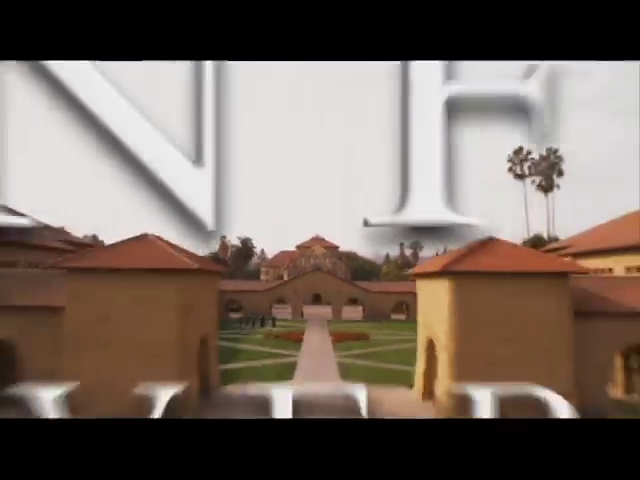
\includegraphics[width=0.78\textwidth]{lecture_02_figure_01.png}
  \caption{Règles de différences finies et de sommes de Riemann à garder au tableau pour la limite continue utilisée plus loin.}
  \lectureframe{00:04:20}
  \label{fig:l02-calculus-board}
\end{figure}

Ce sont les définitions usuelles du calcul différentiel. Leur importance ici tient à leur comportement d’échelle : \(\Delta x_i\) apporte un facteur \(\Delta\sigma\), tandis qu’une somme apporte un facteur inverse lorsqu’elle devient une intégrale.

\subsection{Extrémités de Dirichlet et de Neumann}

L’analyse de Fourier sur un intervalle fini commence par le choix des conditions aux extrémités. Deux choix reviendront souvent.

\begin{align}
  \text{Dirichlet:}\qquad
  &x(0)=x(\pi)=0,
  \label{eq:l02-dirichlet}\\
  \text{Neumann:}\qquad
  &\left.\partial_\sigma x\right|_{\sigma=0}
   =
   \left.\partial_\sigma x\right|_{\sigma=\pi}
   =0.
  \label{eq:l02-neumann}
\end{align}

Une corde de violon fixée aux deux extrémités illustre le cas de Dirichlet : son déplacement s’annule aux bords. Une fonction de Neumann n’a pas besoin de s’y annuler ; sa pente est nulle à chaque bord. Les deux formes caractéristiques sont représentées ensemble au tableau.

\begin{figure}[H]
  \centering
  \begin{minipage}[t]{0.48\textwidth}
    \centering
    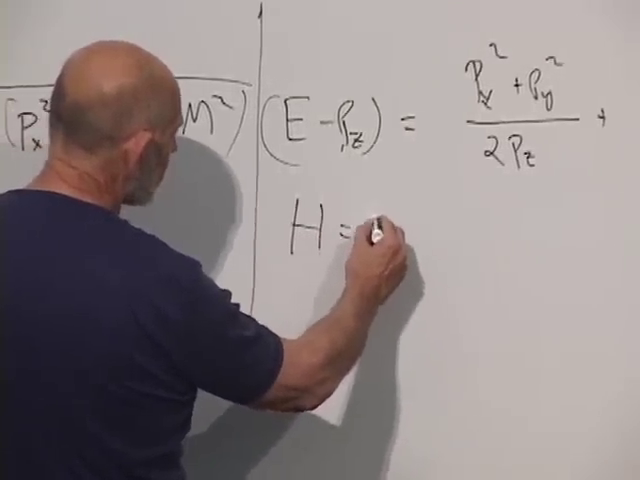
\includegraphics[width=\textwidth]{lecture_02_figure_02.png}
    \par\smallskip\footnotesize (a) Profils à extrémités fixées et de pente nulle.
  \end{minipage}\hfill
  \begin{minipage}[t]{0.48\textwidth}
    \centering
    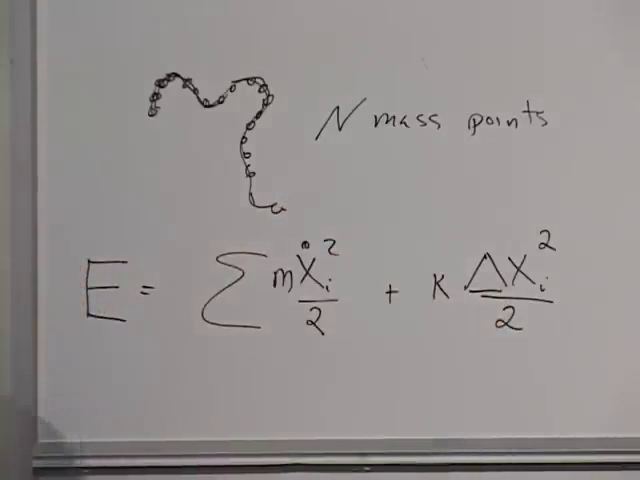
\includegraphics[width=\textwidth]{lecture_02_figure_03.png}
    \par\smallskip\footnotesize (b) Anneaux légers qui coulissent sur des tiges verticales.
  \end{minipage}
  \caption{Les conditions aux limites représentées par des formes et par un dispositif mécanique. Le dispositif des anneaux coulissants donne un sens mécanique sans ambiguïté au mouvement transverse d’une extrémité libre.}
  \lectureframe{00:08:50 and 00:12:15}
  \label{fig:l02-boundaries-board}
\end{figure}

\begin{figure}[H]
  \centering
  \begin{adjustbox}{max width=\linewidth}
  \begin{tikzpicture}[>=Latex,thick,scale=0.92]
    \begin{scope}
      \draw[->] (0,0) -- (4.4,0) node[right] {\(\sigma\)};
      \draw[->] (0,-1.25) -- (0,1.35) node[above] {\(x\)};
      \draw[blue!70!black]
        (0,0) .. controls (0.8,1.1) and (1.4,1.0) .. (2.0,0)
        .. controls (2.7,-1.0) and (3.4,-0.8) .. (4.1,0);
      \fill (0,0) circle (0.06);
      \fill (4.1,0) circle (0.06);
      \node at (2.05,-1.65) {Dirichlet: \(x=0\)};
    \end{scope}
    \begin{scope}[xshift=5.8cm]
      \draw[->] (0,0) -- (4.4,0) node[right] {\(\sigma\)};
      \draw[->] (0,-1.25) -- (0,1.35) node[above] {\(x\)};
      \draw[orange!85!black]
        (0,0.65) .. controls (0.8,0.65) and (1.1,-0.9) .. (2.0,-0.9)
        .. controls (2.9,-0.9) and (3.2,0.55) .. (4.1,0.55);
      \draw[orange!85!black] (0,0.65) -- (0.45,0.65);
      \draw[orange!85!black] (3.65,0.55) -- (4.1,0.55);
      \node at (2.05,-1.65) {Neumann: \(\partial_\sigma x=0\)};
    \end{scope}
  \end{tikzpicture}
  \end{adjustbox}
  \caption{Pour une condition de Dirichlet, la valeur est fixée ; pour une condition de Neumann, c’est la pente qui l’est.}
  \label{fig:l02-boundaries-redraw}
\end{figure}

\begin{classroomqa}
\audiencequestion{Un tuyau d’orgue ouvert ou fermé fournit-il un exemple simple de l’une de ces conditions aux limites ?\lecturetimestamp{00:09:19}}
\lecturerresponse{C’est possible, mais il faut d’abord préciser quelle variable acoustique est développée. La perturbation de pression et le déplacement longitudinal satisfont des conditions idéalisées complémentaires à une extrémité ouverte. Plutôt que de trancher cette question secondaire au tableau, utilisons le modèle des anneaux coulissants : des anneaux presque sans masse peuvent se déplacer verticalement sur les tiges, de sorte que les extrémités de la corde sont libres et que le cas de Neumann s’interprète directement.}
\end{classroomqa}

\begin{classroomqa}
\audiencequestion{Le graphe peut-il avoir une tangente verticale et présenter un saut brutal ?\lecturetimestamp{00:09:53}}
\lecturerresponse{L’analyse de Fourier admet des sauts isolés dans une fonction par morceaux continue. Une corde physique impose des contraintes plus fortes. Un saut disjoint deux points voisins et rend la dérivée spatiale \(\partial_\sigma x\) singulière dans l’énergie continue que nous établirons plus loin. Nous nous limitons donc aux profils continus et dérivables.}
\end{classroomqa}

\begin{classroomqa}
\audiencequestion{Pourquoi l’extrémité ouverte d’un tuyau, ou toute extrémité libre, doit-elle satisfaire une condition aux limites ?\lecturetimestamp{00:11:14}}
\lecturerresponse{L’exemple acoustique dépend du champ choisi et la discussion n’a pas tranché la question. L’exemple mécanique, lui, ne laisse pas d’ambiguïté. Un anneau très léger peut coulisser librement, tout en restant attaché au dernier segment de corde. Nous allons déduire sa condition à partir de la loi de Newton plutôt que de la postuler : une accélération finie à l’extrémité impose que la pente s’annule.}
\end{classroomqa}

\subsection{Les bases de Fourier}

Une fois fixée la classe de conditions aux extrémités, la base de Fourier correspondante est déterminée. Sur \(0\leq\sigma\leq\pi\),

\begin{align}
  x_D(\sigma)
  &=
  \sum_{n=1}^{\infty}x_n\sin(n\sigma),
  \label{eq:l02-dirichlet-series}\\
  x_N(\sigma)
  &=
  \sum_{n=0}^{\infty}x_n\cos(n\sigma).
  \label{eq:l02-neumann-series}
\end{align}

Tous les sinus de \eqref{eq:l02-dirichlet-series} s’annulent aux deux extrémités. Toutes les fonctions cosinus de \eqref{eq:l02-neumann-series} ont une dérivée nulle aux extrémités. Les bornes inférieures diffèrent pour une raison : \(\sin(0\sigma)=0\) ne contribue pas, tandis que \(\cos(0\sigma)=1\) est le mode constant, ou nul. Il représente la valeur moyenne d’une fonction de Neumann.

\begin{figure}[H]
  \centering
  \begin{minipage}[t]{0.48\textwidth}
    \centering
    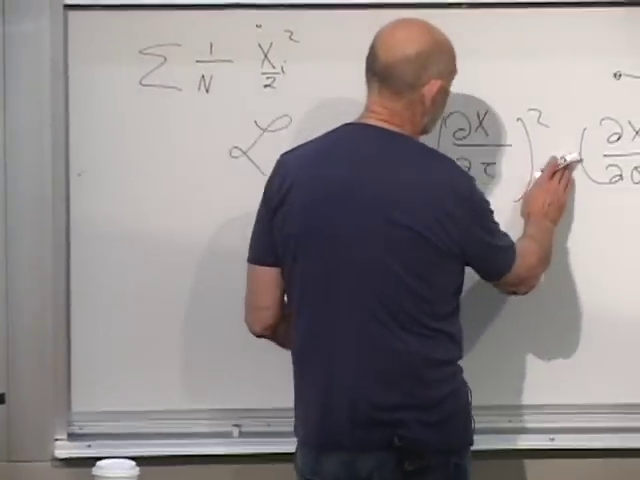
\includegraphics[width=\textwidth]{lecture_02_figure_04.png}
    \par\smallskip\footnotesize (a) Développements en sinus et en cosinus.
  \end{minipage}\hfill
  \begin{minipage}[t]{0.48\textwidth}
    \centering
    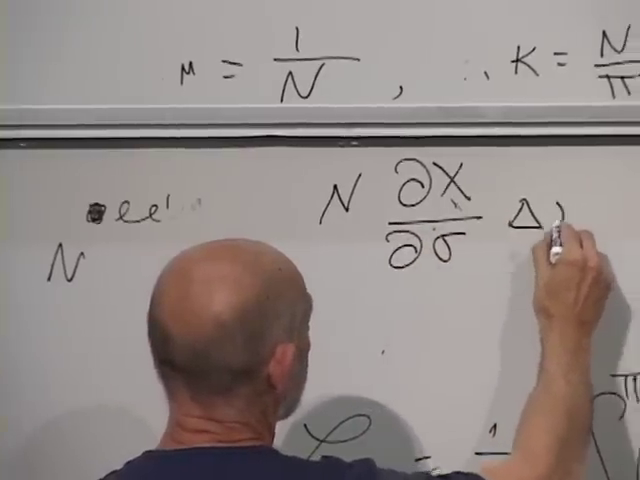
\includegraphics[width=\textwidth]{lecture_02_figure_05.png}
    \par\smallskip\footnotesize (b) Orthogonalité et mode constant exceptionnel.
  \end{minipage}
  \caption{Propriétés de Fourier utilisées plus loin pour diagonaliser la corde.}
  \lectureframe{00:16:15 and 00:20:30}
  \label{fig:l02-fourier-board}
\end{figure}

La dérivation échange les deux classes :

\begin{equation}
  \begin{aligned}
    \partial_\sigma\sin(n\sigma)&=n\cos(n\sigma),\\
    \partial_\sigma\cos(n\sigma)&=-n\sin(n\sigma).
  \end{aligned}
  \label{eq:l02-basis-derivatives}
\end{equation}

Ainsi, la dérivée d’une série de Dirichlet a un comportement de Neumann, et celle d’une série de Neumann a un comportement de Dirichlet. L’orthogonalité élimine alors les termes croisés entre modes distincts :

\begin{align}
  \int_0^\pi\cos(n\sigma)\cos(m\sigma)\,d\sigma
  &=
  \frac{\pi}{2}\delta_{nm},
  && n,m\geq1,
  \label{eq:l02-cos-orthogonality}\\
  \int_0^\pi\sin(n\sigma)\sin(m\sigma)\,d\sigma
  &=
  \frac{\pi}{2}\delta_{nm},
  && n,m\geq1,
  \label{eq:l02-sin-orthogonality}\\
  \int_0^\pi 1\,d\sigma&=\pi .
  \label{eq:l02-zero-norm}
\end{align}

La dernière ligne donne la norme exceptionnelle du cosinus \(n=m=0\). Une constante n’est pas normalisée comme un harmonique non nul ; ce facteur deux distinguera le mode du centre de masse de la corde de ses modes internes.

\subsection{Une formule d’oscillateur à retenir}

Après avoir redimensionné une coordonnée de sorte que la masse mécanique vaille un, un oscillateur obéissant à la loi de Hooke a pour énergie

\begin{align}
  E_{\mathrm{osc}}
  &=
  \frac12\dot q^{\,2}
  +\frac12\omega^2q^2,
  \label{eq:l02-oscillator-energy}\\
  L_{\mathrm{osc}}
  &=
  \frac12\dot q^{\,2}
  -\frac12\omega^2q^2.
  \label{eq:l02-oscillator-lagrangian}
\end{align}

\begin{figure}[H]
  \centering
  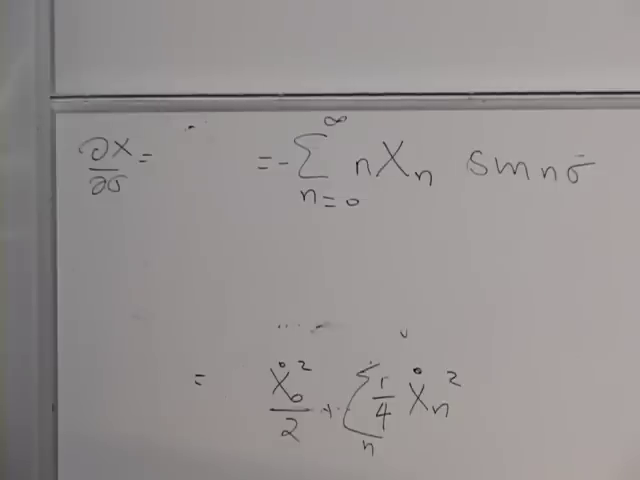
\includegraphics[width=0.68\textwidth]{lecture_02_figure_06.png}
  \caption{L’énergie de l’oscillateur, écrite de façon que le coefficient de \(q^2\) identifie immédiatement \(\omega^2\).}
  \lectureframe{00:24:00}
  \label{fig:l02-oscillator-board}
\end{figure}

Classiquement, \(\omega=\sqrt{\kappa/m}\) ; le redimensionnement de la coordonnée a fixé \(m=1\). En mécanique quantique,

\begin{equation}
  E_Q=\hbar\omega\left(Q+\frac12\right),
  \qquad Q=0,1,2,\ldots .
  \label{eq:l02-oscillator-spectrum}
\end{equation}

Pour les écarts entre niveaux, nous pouvons soustraire le terme commun d’énergie de l’état fondamental et dire que chaque quantum coûte \(\hbar\omega\). Le calcul de la corde procédera d’abord exactement ainsi et remettra à plus tard l’énergie totale du point zéro.

\begin{classroomqa}
\audiencequestion{Comment lit-on la fréquence de l’oscillateur dans la formule de l’énergie ?\lecturetimestamp{00:23:21}}
\lecturerresponse{Avant le redimensionnement, elle vaut \(\omega=\sqrt{\kappa/m}\). Pour une masse unité, le terme de potentiel est \(\frac12\omega^2q^2\) ; son coefficient quadratique est donc le carré de la fréquence.}
\end{classroomqa}

\section{Qu’est-ce qui fait d’un système composite une particule ?}

Une corde est étendue et sera modélisée par de nombreux éléments couplés. En quel sens l’un de ses états quantiques peut-il néanmoins être une particule ? La ponctualité ne peut pas être le critère décisif. Les protons et les neutrons sont composites. Les électrons et les photons sont accompagnés d’un habillage dû aux champs quantiques, bien qu’aucune sous-structure intrinsèque n’ait été mise en évidence. L’image d’un point géométrique classique entouré de rien ne convient pas à une excitation quantique.

La masse et la position du centre de masse ne suffisent pas non plus. Une boîte de gaz possède les deux. Une tasse de café aussi. Pourtant, on n’appelle normalement ni l’une ni l’autre une particule. L’indivisibilité ne convient pas davantage, car un proton est divisible, et le spin ne distingue pas les particules microscopiques des corps macroscopiques.

Le critère utile est l’isolement spectral. Plaçons l’énergie au repos sur un axe vertical et demandons-nous quelle énergie est nécessaire pour atteindre un autre état interne. Juste au-dessus de l’électron, il n’existe pas de série d’excitations électroniques accessible expérimentalement. Le proton, lui, possède des résonances, mais les premières coûtent quelques centaines de MeV, soit une fraction importante de la masse du proton. Ces états sont suffisamment séparés pour être identifiables individuellement.

Une tasse de café, c’est l’inverse. On peut ajouter une énergie arbitrairement petite à un mode sonore de grande longueur d’onde, bousculer une molécule ou produire un phonon. Un nombre immense d’états se pressent dans un intervalle minuscule. À l’échelle du laboratoire, ils forment un continuum. C’est la distinction pratique entre une particule et la \emph{matière informe}.

\begin{figure}[H]
  \centering
  \includegraphics[width=0.58\textwidth]{lecture_02_figure_07.png}
  \caption{Axe vertical de l’énergie au tableau, lors de la comparaison entre le niveau isolé d’une particule et les excitations denses de la matière ordinaire.}
  \lectureframe{00:31:10}
  \label{fig:l02-spectrum-board}
\end{figure}

\begin{figure}[H]
  \centering
  \begin{adjustbox}{max width=\linewidth}
  \begin{tikzpicture}[>=Latex,thick]
    \begin{scope}
      \draw[->] (0,0) -- (0,4.8) node[above] {energy};
      \draw[blue!70!black,line width=1.2pt] (-1.0,0.65) -- (1.0,0.65);
      \draw[blue!70!black,line width=1.2pt] (-1.0,3.65) -- (1.0,3.65);
      \node[right] at (1.05,0.65) {ground state};
      \node[right] at (1.05,3.65) {first internal excitation};
      \draw[<->] (0.65,0.75) -- (0.65,3.55)
        node[midway,right] {large gap};
      \node at (0,-0.55) {particle-like};
    \end{scope}
    \begin{scope}[xshift=7.0cm]
      \draw[->] (0,0) -- (0,4.8) node[above] {energy};
      \foreach \y in {0.55,0.69,0.82,0.94,1.05,1.15,1.24,1.32,1.39,1.45,
        1.51,1.57,1.63,1.70,1.78,1.87,1.97,2.09,2.22,2.36,2.51,2.67,2.84,
        3.02,3.21,3.41,3.62,3.84,4.07}
        \draw[orange!85!black] (-0.95,\y) -- (0.95,\y);
      \node[right] at (1.05,2.25) {dense phonon and internal states};
      \node at (0,-0.55) {macroscopic matter};
    \end{scope}
  \end{tikzpicture}
  \end{adjustbox}
  \caption{Dans ce cours, le critère opérationnel de particule est l’isolement spectral, et non la ponctualité au sens littéral.}
  \label{fig:l02-particle-redraw}
\end{figure}

Ce critère transforme la question philosophique en calcul. Quantifions la corde, déterminons ses niveaux d’énergie internes et examinons leurs espacements. Si le premier état excité de la corde se situe près de l’échelle de Planck tandis que l’état fondamental observé est léger, le gap dépasse de plus de vingt ordres de grandeur les énergies actuelles des accélérateurs. Dans tout le domaine accessible, la corde se comporte alors comme une particule élémentaire.

\begin{classroomqa}
\audiencequestion{Le comportement particulaire dépend-il simplement de l’échelle d’observation ? Si l’on zoome suffisamment, les niveaux cessent-ils d’être distincts ?\lecturetimestamp{00:33:33}}
\lecturerresponse{Un examen à plus petite échelle peut révéler qu’un objet comporte de nombreux constituants, mais il n’efface pas le spectre. La comparaison pertinente porte sur la résolution en énergie de l’expérience et le gap jusqu’à la première excitation interne. Un objet composite peut conserver un comportement particulaire lorsque ce gap est immense.}
\end{classroomqa}

\begin{classroomqa}
\audiencequestion{Pourquoi une corde de violon ordinaire n’est-elle pas une particule ?\lecturetimestamp{00:34:37}}
\lecturerresponse{L’énergie d’un quantum de vibration est incommensurablement petite par rapport à l’énergie au repos de la corde macroscopique. De nombreux états quantiques tiennent donc dans un intervalle relatif minuscule. La corde relève du côté du spectre dense, et non du côté des niveaux isolés.}
\end{classroomqa}

\begin{classroomqa}
\audiencequestion{Les photons et les électrons sont-ils des particules ponctuelles si des fluctuations virtuelles entourent les champs quantiques ?\lecturetimestamp{00:35:40}}
\lecturerresponse{Le mot classique \emph{ponctuel} recouvre trop de choses. L’électron et le photon physiques sont des excitations habillées des champs, mais les expériences n’ont révélé pour aucun des deux de structure intrinsèque en constituants ni de facteur de forme fini. Pour le présent argument, l’essentiel est qu’aucun ne possède une série dense d’états internes presque dégénérés.\editorialnote{Le cours associe le moment magnétique anomal de l’électron à un flou quantique mesurable. Dans la terminologie moderne, ce moment anomal est un effet d’habillage radiatif, et non la preuve d’un rayon fini de l’électron qui aurait été résolu. Par convention, « ponctuel » signifie qu’aucune sous-structure intrinsèque ni aucun facteur de forme n’a été détecté jusqu’à l’échelle sondée.}}
\end{classroomqa}

\begin{classroomqa}
\audiencequestion{La taille d’un photon dépend-elle de sa fréquence ?\lecturetimestamp{00:36:49}}
\lecturerresponse{Sa longueur d’onde, certainement. C’est une notion distincte de la taille intrinsèque de ses constituants. Changer la fréquence modifie le paquet d’ondes et sa longueur d’onde, mais pas un rayon interne du photon qui aurait été résolu.}
\end{classroomqa}

\section{Mécanique transverse exacte à grande impulsion}

Revenons maintenant à la difficulté relativiste. On ne peut pas traiter un bâton en rotation rapide de façon non relativiste en plaçant simplement son centre de masse au repos. Ses extrémités continuent de se déplacer l’une par rapport à l’autre à des vitesses relativistes. C’est le mouvement relatif interne qui rend l’approximation non relativiste invalide.

Il existe cependant une autre limite. Choisissons un axe \(z\) et effectuons une transformation de Lorentz de l’ensemble du système vers une très grande impulsion longitudinale positive \(P_z\). Gardons son impulsion transverse

\begin{equation}
  p_\perp^2=p_x^2+p_y^2
\end{equation}

finie. La projection transverse admet alors une forme hamiltonienne exactement non relativiste dans la limite \(P_z\to\infty\), même si le mouvement interne avant la transformation de Lorentz était relativiste.

\begin{classroomqa}
\audiencequestion{À impulsion infinie, le système massif atteint-il réellement la vitesse de la lumière ?\lecturetimestamp{00:40:43}}
\lecturerresponse{Aucune transformation de Lorentz finie ne l’y amène. On construit des quantités qui ont des limites bien définies lorsque \(P_z\) devient arbitrairement grande. L’expression désigne une procédure limite, et non un état physique à impulsion finie où \(v=c\).}
\end{classroomqa}

\begin{classroomqa}
\audiencequestion{Quel axe faut-il choisir, et qu’en est-il si l’objet tourne autour de cet axe ou dans sa direction transverse ?\lecturetimestamp{00:41:14}}
\lecturerresponse{On peut choisir n’importe quel axe et effectuer la transformation de Lorentz de l’ensemble du système dans cette direction. La mécanique qui reste explicitement en jeu est la projection sur le plan perpendiculaire. Une tige en rotation peut sembler raccourcie ou balayer ce plan, mais sa projection transverse a une forme non relativiste.}
\end{classroomqa}

Les cordes possèdent une propriété supplémentaire qui rend cette représentation particulièrement puissante. En jauge du front de lumière, leurs coordonnées internes longitudinales ne sont pas des oscillateurs indépendants. Les contraintes les déterminent à partir du mouvement transverse. Connaître la corde transverse suffit donc à reconstruire les degrés de liberté physiques.

\begin{classroomqa}
\audiencequestion{L’absence de coordonnée longitudinale indépendante signifie-t-elle que la corde est simplement prise en sandwich dans une couche mince ?\lecturetimestamp{00:42:26}}
\lecturerresponse{La contraction de Lorentz rend effectivement son étendue longitudinale faible dans le référentiel transformé, mais l’affirmation va plus loin. Tout mouvement longitudinal résiduel est contraint par le mouvement transverse ; il ne peut pas être spécifié indépendamment.}
\end{classroomqa}

\begin{classroomqa}
\audiencequestion{Cette réduction aux données transverses est-elle liée au principe holographique ?\lecturetimestamp{00:43:12}}
\lecturerresponse{Elle est étroitement liée au cheminement qui a conduit aux idées holographiques, mais développer ce lien nous éloignerait du calcul présent. Ici, elle justifie simplement de travailler avec la corde transverse.}
\end{classroomqa}

\subsection{Soustraire l’impulsion de la transformation de Lorentz et redimensionner le temps}

Soit \(M\) la masse invariante du système complet, qui inclut les masses des constituants, l’énergie cinétique et l’énergie de liaison. Dans les unités où \(c=1\),

\begin{equation}
  E=\sqrt{P_z^2+p_\perp^2+M^2}.
  \label{eq:l02-relativistic-energy}
\end{equation}

Pour \(P_z\) très grand devant \(p_\perp\) et \(M\),

\begin{equation}
  E
  =
  P_z+\frac{p_\perp^2+M^2}{2P_z}
  +O(P_z^{-3}).
  \label{eq:l02-large-pz}
\end{equation}

\begin{figure}[H]
  \centering
  \includegraphics[width=0.76\textwidth]{lecture_02_figure_08.png}
  \caption{Développement à grande valeur de \(P_z\), avec l’impulsion transverse et la masse invariante conservées.}
  \lectureframe{00:47:30}
  \label{fig:l02-large-pz-board}
\end{figure}

Le terme dominant est grand, mais ne contient aucune information sur l’état interne. Dans un processus qui conserve \(P_z\), comme le passage d’un atome soumis à une transformation de Lorentz entre deux niveaux internes sans changement de son impulsion longitudinale totale, ce terme s’élimine de chaque différence d’énergie. Nous étudions donc

\begin{equation}
  E-P_z=\frac{p_\perp^2+M^2}{2P_z}+O(P_z^{-3}).
  \label{eq:l02-residual-energy}
\end{equation}

Le dénominateur a une signification physique. Comme le hamiltonien engendre l’évolution temporelle, la faible énergie résiduelle indique que l’évolution interne paraît lente dans le temps du laboratoire. C’est la dilatation du temps. Pour conserver le mouvement interne, introduisons un paramètre d’évolution redimensionné \(\tau\), ou, de façon équivalente, multiplions le hamiltonien résiduel par \(P_z\) :

\begin{equation}
  H_\perp
  \equiv
  \lim_{P_z\to\infty}P_z(E-P_z)
  =
  \frac12p_\perp^2+\frac12M^2.
  \label{eq:l02-transverse-hamiltonian}
\end{equation}

\begin{figure}[H]
  \centering
  \begin{minipage}[t]{0.48\textwidth}
    \centering
    \includegraphics[width=\textwidth]{lecture_02_figure_09.png}
    \par\smallskip\footnotesize (a) \(H=i\partial_t\) et le ralentissement de l’évolution interne.
  \end{minipage}\hfill
  \begin{minipage}[t]{0.48\textwidth}
    \centering
    \includegraphics[width=\textwidth]{lecture_02_figure_10.png}
    \par\smallskip\footnotesize (b) Le hamiltonien transverse fini après redimensionnement du temps.
  \end{minipage}
  \caption{De l’énergie résiduelle dilatée dans le temps à un hamiltonien bidimensionnel fini.}
  \lectureframe{00:49:20 and 00:52:40}
  \label{fig:l02-lightfront-board}
\end{figure}

C’est exactement la forme de l’énergie d’une particule de masse unité se déplaçant en deux dimensions : énergie cinétique \(p_\perp^2/2\) plus énergie interne \(M^2/2\). La particularité tient au carré. Dans cette description, la quantité qui joue le rôle de l’énergie au repos ou de liaison est proportionnelle au carré de la masse invariante.\editorialnote{Avec les variables usuelles du front de lumière \(P^\pm=(E\pm P_z)/\sqrt2\), la relation exacte de couche de masse est \(2P^+P^-=p_\perp^2+M^2\). L’équation \eqref{eq:l02-transverse-hamiltonian} correspond à la normalisation à grande valeur de \(P_z\), utilisée dans le cours, de cette même relation invariante.}

\begin{classroomqa}
\audiencequestion{Qu’advient-il des impulsions longitudinales des différentes parties d’un système composite ?\lecturetimestamp{00:51:30}}
\lecturerresponse{Pour un objet composite générique, il faut conserver les fractions de l’impulsion totale \(P_z\) portées par ses constituants. La formule ci-dessus fait intervenir l’impulsion totale du centre de masse. La théorie des cordes est particulière : ses contraintes déterminent le mouvement longitudinal relatif à partir des degrés de liberté transverses, si bien qu’il n’est pas nécessaire d’ajouter un oscillateur longitudinal indépendant.}
\end{classroomqa}

\section{Une corde ouverte discrète}

La corde transformée de Lorentz ne se déplace désormais explicitement que dans le plan transverse. Désignons ses deux coordonnées par \(X\) et \(Y\) et commençons par l’approximer par \(N\) points matériels reliés par \(N-1\) ressorts. Si \(\mu\) est la masse analogue de chaque point et \(k\) la constante de raideur des ressorts entre voisins immédiats, l’énergie vaut

\begin{equation}
  E_N
  =
  \sum_i
  \left[
    \frac{\mu}{2}
    \left(\dot X_i^2+\dot Y_i^2\right)
    +
    \frac{k}{2}
    \left((\Delta X_i)^2+(\Delta Y_i)^2\right)
  \right].
  \label{eq:l02-discrete-energy}
\end{equation}

Chaque terme en \(X\) s’accompagne d’un terme identique en \(Y\), car le plan transverse a deux directions. L’indice \(i\) repère un point le long de la chaîne ; ce n’est pas une coordonnée spatiale.

\begin{figure}[H]
  \centering
  \begin{minipage}[t]{0.48\textwidth}
    \centering
    \includegraphics[width=\textwidth]{lecture_02_figure_11.png}
    \par\smallskip\footnotesize (a) Chaîne de billes et énergie discrète.
  \end{minipage}\hfill
  \begin{minipage}[t]{0.48\textwidth}
    \centering
    \includegraphics[width=\textwidth]{lecture_02_figure_12.png}
    \par\smallskip\footnotesize (b) Comportement à grande valeur de \(N\) pour \(\mu\) et \(k\).
  \end{minipage}
  \caption{La corde ouverte régularisée avant la limite continue.}
  \lectureframe{00:57:42 and 01:02:40}
  \label{fig:l02-chain-board}
\end{figure}

\begin{figure}[H]
  \centering
  \begin{adjustbox}{max width=\linewidth}
  \begin{tikzpicture}[>=Latex,thick]
    \foreach \i in {0,...,8} {
      \coordinate (p\i) at ({1.05*\i},{0.30*sin(55*\i)});
      \filldraw[white] (p\i) circle (0.10);
      \draw (p\i) circle (0.10);
    }
    \foreach \i in {0,...,7} {
      \pgfmathtruncatemacro{\j}{\i+1}
      \draw[decorate,decoration={zigzag,segment length=4pt,amplitude=2pt}]
        (p\i) -- (p\j);
    }
    \node[above=0.35cm of p0] {\(i=0\)};
    \node[above=0.35cm of p8] {\(i=N-1\)};
    \draw[<->] (0,-1.15) -- (8.4,-1.15)
      node[midway,below] {\(0\leq\sigma\leq\pi\)};
    \node at (4.2,1.25)
      {\(\mu=1/N,\quad k=N/\pi^2,\quad\Delta\sigma=\pi/N\)};
  \end{tikzpicture}
  \end{adjustbox}
  \caption{Une image claire de la régularisation. À mesure que la chaîne est affinée, les points s’allègent et les ressorts microscopiques se raidissent.}
  \label{fig:l02-chain-redraw}
\end{figure}

Le paramètre \(\sigma\) repère la position le long de la chaîne. Choisir \(0\leq\sigma\leq\pi\) relève d’une convention, et non d’une mesure de longueur physique. Cela nous rappelle que la corde a deux extrémités. Plus tard, une corde fermée sera paramétrée périodiquement sur \(0\leq\sigma<2\pi\).

La limite continue doit conserver une mécanique collective finie. Une masse fixe pour chaque bille ferait diverger la masse analogue totale ; choisissons donc

\begin{equation}
  \mu=\frac{1}{N}.
  \label{eq:l02-mu-scaling}
\end{equation}

Alors \(N\mu=1\). Il ne s’agit pas de la masse au repos relativiste \(M\), mais du coefficient d’inertie dans le modèle transverse analogue.

Des ressorts montés en série s’assouplissent lorsque leur nombre augmente. Pour conserver une raideur finie à l’échelle de toute la chaîne, chaque ressort microscopique doit donc se raidir :

\begin{equation}
  k=\frac{N}{\pi^2}
  =\frac{1}{\pi\,\Delta\sigma}.
  \label{eq:l02-k-scaling}
\end{equation}

Seule \(k\propto N\) est essentielle. Le facteur \(\pi^2\) est une normalisation choisie pour éliminer les facteurs \(\pi\) indésirables dans les formules continues.

\begin{classroomqa}
\audiencequestion{\(\mu\) est-elle la masse au repos physique de chaque point de la corde ?\lecturetimestamp{01:10:34}}
\lecturerresponse{Non. C’est la masse analogue non relativiste qui intervient dans la chaîne transverse. L’appeler \(M\) risquerait de la confondre avec la masse au repos invariante de l’état relativiste complet de la corde. Pour l’instant, elle sert uniquement à obtenir l’inertie continue correcte.}
\end{classroomqa}

\section{Le système d’ondes continu}

Appliquons les règles établies au début. Puisque \(1/N=\Delta\sigma/\pi\),

\begin{align}
  \sum_i\frac{\mu}{2}\dot X_i^2
  &=
  \frac{1}{2\pi}
  \sum_i\dot X_i^2\,\Delta\sigma
  \longrightarrow
  \frac{1}{2\pi}
  \int_0^\pi
  \left(\partial_\tau X\right)^2d\sigma ,
  \label{eq:l02-kinetic-limit}\\
  \sum_i\frac{k}{2}(\Delta X_i)^2
  &\longrightarrow
  \frac{1}{2\pi}
  \int_0^\pi
  \left(\partial_\sigma X\right)^2d\sigma .
  \label{eq:l02-potential-limit}
\end{align}

Pour la deuxième ligne, utilisons \(\Delta X_i=\partial_\sigma X\,\Delta\sigma\) ainsi que \(k=1/(\pi\Delta\sigma)\). Le même calcul s’applique à \(Y\).

\begin{figure}[H]
  \centering
  \begin{minipage}[t]{0.48\textwidth}
    \centering
    \includegraphics[width=\textwidth]{lecture_02_figure_13.png}
    \par\smallskip\footnotesize (a) Passage de la somme à l’intégrale et de la différence à la dérivée.
  \end{minipage}\hfill
  \begin{minipage}[t]{0.48\textwidth}
    \centering
    \includegraphics[width=\textwidth]{lecture_02_figure_14.png}
    \par\smallskip\footnotesize (b) Énergie continue obtenue.
  \end{minipage}
  \caption{La chaîne discrète devient un champ sur l’intervalle \(\sigma\).}
  \lectureframe{01:05:40 and 01:07:00}
  \label{fig:l02-continuum-board}
\end{figure}

L’énergie et le lagrangien obtenus sont

\begin{align}
  E
  &=
  \frac{1}{2\pi}
  \int_0^\pi d\sigma\,
  \left[
    (\partial_\tau X)^2+(\partial_\tau Y)^2\right.\notag\\[-0.25em]
  &\hspace{6.5em}\left.
    +(\partial_\sigma X)^2+(\partial_\sigma Y)^2
  \right],
  \label{eq:l02-continuum-energy}\\
  L
  &=
  \frac{1}{2\pi}
  \int_0^\pi d\sigma\,
  \left[
    (\partial_\tau X)^2+(\partial_\tau Y)^2\right.\notag\\[-0.25em]
  &\hspace{6.5em}\left.
    -(\partial_\sigma X)^2-(\partial_\sigma Y)^2
  \right].
  \label{eq:l02-continuum-lagrangian}
\end{align}

\begin{figure}[H]
  \centering
  \includegraphics[width=0.78\textwidth]{lecture_02_figure_15.png}
  \caption{Le lagrangien continu, dont les termes cinétique et d’étirement ont des signes opposés.}
  \lectureframe{01:08:48}
  \label{fig:l02-lagrangian-board}
\end{figure}

Si nous rebaptisons \(\sigma\) coordonnée spatiale ordinaire et \(X\) champ \(\phi\), nous obtenons l’énergie et le lagrangien d’un champ d’ondes unidimensionnel. La variation de \eqref{eq:l02-continuum-lagrangian} donne

\begin{equation}
  \left(\partial_\tau^2-\partial_\sigma^2\right)X=0,
  \qquad
  \left(\partial_\tau^2-\partial_\sigma^2\right)Y=0.
  \label{eq:l02-wave-equation}
\end{equation}

Rien dans l’argument immédiat ne nous oblige à résoudre directement ces équations. Il suffit de se représenter des ondes qui se propagent vers la gauche et vers la droite le long de la corde et se réfléchissent à ses extrémités. Une réflexion de Dirichlet inverse le signe du déplacement ; une réflexion de Neumann le conserve.

\begin{classroomqa}
\audiencequestion{Que représente exactement la variable temporelle \(\tau\)\lecturetimestamp{01:08:54}}
\lecturerresponse{C’est le temps redimensionné utilisé pour suivre le mouvement interne dans la description à grande valeur de \(P_z\). Une horloge entraînée avec le système avance lentement par rapport au temps du laboratoire ; \(\tau\) élimine cette dilatation afin que les oscillations internes conservent une fréquence finie. Pour cette mécanique transverse, on peut simplement le traiter comme le temps.\editorialnote{Le cours appelle informellement \(\tau\) le temps propre. Pour une corde étendue, le paramètre d’évolution précis du front de lumière est un temps redimensionné après fixation de jauge, et non un temps propre invariant unique partagé par tous les points. Cela ne change rien à l’argument visé sur la dilatation du temps.}}
\end{classroomqa}

Lorsque le centre de masse est au repos dans le plan transverse, la partie interne de \eqref{eq:l02-continuum-energy} est, dans la normalisation de \eqref{eq:l02-transverse-hamiltonian}, proportionnelle à \(M^2\). C’est pourquoi la quantification de ce système d’ondes apparemment ordinaire révélera le spectre de masse relativiste.

\begin{classroomqa}
\audiencequestion{\(P_z(E-P_z)\) porte-t-il un nom ?\lecturetimestamp{01:11:00}}
\lecturerresponse{On l’appelle couramment énergie du cône de lumière ou du front de lumière. « Front de lumière » décrit mieux l’hypersurface de genre lumière utilisée comme surface d’évolution ; la terminologie traditionnelle n’a pas d’importance pour le calcul.}
\end{classroomqa}

\begin{classroomqa}
\audiencequestion{Le mot « cône » désigne-t-il le cône de lumière usuel de l’espace-temps, et Dirac a-t-il introduit cette terminologie ?\lecturetimestamp{01:11:17}}
\lecturerresponse{La construction en coordonnées nulles peut se représenter avec des axes à 45 degrés, mais la surface d’évolution considérée ici est un front de lumière, et non le cône complet en expansion. Dirac a développé des formulations apparentées de la dynamique relativiste ; la question de l’origine historique du terme est restée ouverte et n’influe pas sur les équations.}
\end{classroomqa}

\section{Pourquoi une extrémité libre satisfait la condition de Neumann}

Nous pouvons maintenant déduire la condition aux extrémités au lieu de la postuler. La loi de Newton s’applique, car la mécanique transverse après la transformation de Lorentz a exactement la forme non relativiste. Un point matériel intérieur est tiré par des ressorts des deux côtés. Le point à l’extrémité ne subit la traction que du ressort qui le relie à son voisin.

\begin{classroomqa}
\audiencequestion{Pourquoi pouvons-nous utiliser la loi de Newton tout en étudiant une corde relativiste ?\lecturetimestamp{01:14:52}}
\lecturerresponse{Nous n’appliquons pas la mécanique newtonienne au mouvement complet dans l’espace-temps avant la transformation de Lorentz. Nous l’appliquons aux variables transverses de la description à impulsion infinie, dont le hamiltonien a exactement la forme non relativiste.}
\end{classroomqa}

À l’extrémité droite, la loi de Hooke donne, au signe près selon l’orientation,

\begin{equation}
  F_{\mathrm{end}}
  =
  -k\,\Delta X
  =
  -\frac{1}{\pi\Delta\sigma}
   \left(\partial_\sigma X\,\Delta\sigma\right)
  =
  -\frac{1}{\pi}\partial_\sigma X .
  \label{eq:l02-endpoint-force}
\end{equation}

\begin{figure}[H]
  \centering
  \begin{minipage}[t]{0.48\textwidth}
    \centering
    \includegraphics[width=\textwidth]{lecture_02_figure_16.png}
    \par\smallskip\footnotesize (a) Force à l’extrémité proportionnelle à la pente locale.
  \end{minipage}\hfill
  \begin{minipage}[t]{0.48\textwidth}
    \centering
    \includegraphics[width=\textwidth]{lecture_02_figure_17.png}
    \par\smallskip\footnotesize (b) Condition d’accélération finie.
  \end{minipage}
  \caption{Déduction de la condition aux limites d’extrémité libre à partir de la loi de Newton.}
  \lectureframe{01:18:20 and 01:20:10}
  \label{fig:l02-neumann-board}
\end{figure}

L’équation de Newton pour le point terminal est

\begin{equation}
  \mu\,\partial_\tau^2X=F_{\mathrm{end}},
  \qquad
  \mu=\frac1N=\frac{\Delta\sigma}{\pi}.
  \label{eq:l02-endpoint-newton}
\end{equation}

En combinant \eqref{eq:l02-endpoint-force} et \eqref{eq:l02-endpoint-newton},

\begin{equation}
  \partial_\sigma X
  =
  -\Delta\sigma\,\partial_\tau^2X
  \quad\text{at the right endpoint},
  \label{eq:l02-endpoint-scaling}
\end{equation}

avec le signe de la force inversé à l’extrémité gauche. Si \(\partial_\sigma X\) tendait vers une constante non nulle tandis que \(\Delta\sigma\to0\), l’accélération de l’extrémité divergerait comme \(N\). Une limite continue raisonnable avec accélération finie exige donc

\begin{equation}
  \left.\partial_\sigma X\right|_{0,\pi}=0,
  \qquad
  \left.\partial_\sigma Y\right|_{0,\pi}=0.
  \label{eq:l02-open-neumann}
\end{equation}

\begin{figure}[H]
  \centering
  \begin{adjustbox}{max width=\linewidth}
  \begin{tikzpicture}[>=Latex,thick,scale=1.0]
    \coordinate (a) at (0,0);
    \coordinate (b) at (4.5,0.75);
    \filldraw[white] (a) circle (0.12);
    \draw (a) circle (0.12);
    \filldraw[white] (b) circle (0.12);
    \draw (b) circle (0.12);
    \draw[decorate,decoration={zigzag,segment length=6pt,amplitude=3pt}]
      (a) -- (b);
    \draw[dashed] (a) -- (0,-1.2);
    \draw[dashed] (b) -- (4.5,-1.2);
    \draw[<->] (4.85,0) -- (4.85,0.75)
      node[midway,right] {\(\Delta X\)};
    \draw[->,red!70!black] (b) -- (5.75,0.95)
      node[right] {\(F_{\rm end}=-k\Delta X\)};
    \node[below] at (0,-1.2) {\(N-1\)};
    \node[below] at (4.5,-1.2) {\(N\)};
    \node at (2.5,-2.0)
      {\(\mu\ddot X=-k\Delta X
      \ \Longrightarrow\
      \partial_\sigma X=-\Delta\sigma\,\ddot X\to0\)};
  \end{tikzpicture}
  \end{adjustbox}
  \caption{Dans la limite de régularisation, la masse du dernier point tend vers zéro. Une accélération finie n’est possible que si la pente à l’extrémité s’annule.}
  \label{fig:l02-neumann-redraw}
\end{figure}

Le même argument aux deux extrémités et dans les deux directions transverses donne des conditions aux limites de Neumann pour une corde ouverte libre.

\section{Modes normaux de la corde ouverte}

Nous disposons maintenant d’un système classique complet : un lagrangien et ses conditions aux limites. Après l’analyse de Fourier, la quantification devient simple. Comme les extrémités sont de Neumann,

\begin{align}
  X(\sigma,\tau)
  &=
  \sum_{n=0}^{\infty}X_n(\tau)\cos(n\sigma),
  \label{eq:l02-X-expansion}\\
  Y(\sigma,\tau)
  &=
  \sum_{n=0}^{\infty}Y_n(\tau)\cos(n\sigma).
  \label{eq:l02-Y-expansion}
\end{align}

Toute la dépendance en \(\sigma\) est portée par les cosinus. Toute la dépendance temporelle est portée par les coefficients ; la corde oscille parce que \(X_n(\tau)\) et \(Y_n(\tau)\) varient.

\begin{figure}[H]
  \centering
  \includegraphics[width=0.78\textwidth]{lecture_02_figure_18.png}
  \caption{Développement en modes de Neumann, placé à côté de la relation d’orthogonalité qui réduira les sommes doubles.}
  \lectureframe{01:21:45}
  \label{fig:l02-mode-expansion-board}
\end{figure}

\subsection{Terme cinétique et mode zéro}

La dérivation par rapport au temps donne

\begin{equation}
  \partial_\tau X
  =
  \sum_{n=0}^{\infty}\dot X_n(\tau)\cos(n\sigma).
  \label{eq:l02-time-mode}
\end{equation}

Le carré produit une somme double sur \(n\) et \(m\), mais
\eqref{eq:l02-cos-orthogonality} annule tous les termes pour lesquels \(n\neq m\).
En traitant séparément le mode constant,

\begin{equation}
  \frac{1}{2\pi}\int_0^\pi
  (\partial_\tau X)^2\,d\sigma
  =
  \frac12\dot X_0^{\,2}
  +
  \frac14\sum_{n=1}^{\infty}\dot X_n^{\,2}.
  \label{eq:l02-mode-kinetic}
\end{equation}

\begin{figure}[H]
  \centering
  \includegraphics[width=0.76\textwidth]{lecture_02_figure_19.png}
  \caption{L’intégrale d’orthogonalité réduit la somme double du terme cinétique au mode zéro et à une somme diagonale.}
  \lectureframe{01:29:10}
  \label{fig:l02-mode-kinetic-board}
\end{figure}

Le coefficient constant est la position moyenne,

\begin{equation}
  X_0(\tau)=\frac1\pi\int_0^\pi X(\sigma,\tau)\,d\sigma ,
  \label{eq:l02-center-of-mass}
\end{equation}

et de même pour \(Y_0\). Avec une densité de masse uniforme analogue, ces coordonnées sont celles du centre de masse. Elles ont une énergie cinétique, mais aucune force de rappel : la corde entière peut se déplacer librement dans le plan transverse.

\subsection{Terme d’étirement et fréquences des oscillateurs}

La dérivation spatiale donne

\begin{equation}
  \partial_\sigma X
  =
  -\sum_{n=1}^{\infty}nX_n(\tau)\sin(n\sigma).
  \label{eq:l02-spatial-mode}
\end{equation}

Le mode zéro disparaît, car une translation uniforme n’étire pas la corde. En utilisant l’orthogonalité des sinus,

\begin{equation}
  \frac{1}{2\pi}\int_0^\pi
  (\partial_\sigma X)^2\,d\sigma
  =
  \frac14\sum_{n=1}^{\infty}n^2X_n^{\,2}.
  \label{eq:l02-mode-potential}
\end{equation}

\begin{figure}[H]
  \centering
  \includegraphics[width=0.76\textwidth]{lecture_02_figure_20.png}
  \caption{La dérivation de la série de cosinus produit la somme double de sinus ; l’orthogonalité impose de nouveau \(n=m\).}
  \lectureframe{01:31:40}
  \label{fig:l02-mode-potential-board}
\end{figure}

Le lagrangien du secteur \(X\) s’écrit donc

\begin{equation}
  L_X
  =
  \frac12\dot X_0^{\,2}
  +
  \frac14\sum_{n=1}^{\infty}
  \left(
    \dot X_n^{\,2}-n^2X_n^{\,2}
  \right),
  \label{eq:l02-X-lagrangian}
\end{equation}

avec une expression identique pour \(Y\). L’énergie correspondante comporte un signe plus devant \(n^2X_n^2\). Chaque mode non nul est un oscillateur harmonique indépendant et, par comparaison avec \eqref{eq:l02-oscillator-lagrangian}, on obtient

\begin{equation}
  \omega_n=n,
  \qquad n=1,2,3,\ldots .
  \label{eq:l02-mode-frequency}
\end{equation}

\begin{figure}[H]
  \centering
  \includegraphics[width=0.80\textwidth]{lecture_02_figure_21.png}
  \caption{Le lagrangien des oscillateurs découplés et la conclusion \(\omega_n=n\), avec la tour identique de \(Y\) indiquée ci-dessous.}
  \lectureframe{01:35:50}
  \label{fig:l02-oscillator-modes-board}
\end{figure}

Les modes normaux sont simplement les harmoniques de la corde. Le premier se courbe lentement, le deuxième a une fréquence deux fois plus élevée, le troisième trois fois plus élevée, et ainsi de suite. Dans la théorie libre, l’orthogonalité empêche tout couplage entre harmoniques.

\begin{classroomqa}
\audiencequestion{Que devient l’oscillateur \(n=0\) ?\lecturetimestamp{01:34:49}}
\lecturerresponse{Sa fréquence est nulle, car il ne s’agit pas du tout d’un oscillateur interne. Il traduit le centre de masse. Aucun ressort ne ramène la corde entière à une position transverse privilégiée : le mode zéro est donc une coordonnée de particule libre.}
\end{classroomqa}

En supprimant le terme cinétique du centre de masse, il reste l’énergie interne

\begin{equation}
  E_{\mathrm{int}}
  =
  \frac14
  \sum_{n=1}^{\infty}
  \left[
    \dot X_n^{\,2}+n^2X_n^{\,2}
    +\dot Y_n^{\,2}+n^2Y_n^{\,2}
  \right].
  \label{eq:l02-internal-energy}
\end{equation}

Dans la normalisation du cône de lumière, cette énergie est proportionnelle au carré de la masse invariante de l’état de la corde. Nous avons ainsi ramené le problème relativiste de la masse à la mécanique quantique de deux tours dénombrables d’oscillateurs.

\section{Niveaux quantifiés et comportement particulaire}

Soit \(a_n^\dagger\) l’opérateur qui crée un quantum dans l’oscillateur \(X\) de fréquence
\(n\), et \(b_n^\dagger\) celui qui fait de même pour \(Y\). Le cours remet à plus tard le traitement systématique des opérateurs, mais cette notation rend le dénombrement des niveaux transparent. Par rapport au décalage de l’état fondamental,

\begin{equation}
  \begin{aligned}
    \Delta E_{\mathrm{int}}
    &=\sum_{n=1}^{\infty}n\left(Q_n^X+Q_n^Y\right),\\
    Q_n^X,Q_n^Y&\in\{0,1,2,\ldots\}.
  \end{aligned}
  \label{eq:l02-quantized-energy}
\end{equation}

où \(\hbar=1\). L’entier \(n\) indique quel oscillateur est excité ;
\(Q_n\) compte le nombre de quanta qu’il contient.\editorialnote{Chaque oscillateur contribue aussi une énergie de point zéro. La somme
infinie nécessite une régularisation et fournit l’intercept de la formule de masse de la corde. Le cours laisse délibérément indéterminé ici le décalage de l’état fondamental et ne dénombre que les niveaux d’excitation.}

Le vide des oscillateurs \(\ket{0}\) n’est pas le vide de l’espace-temps. Il s’agit d’une corde ouverte sans aucun oscillateur interne excité. Elle possède une énergie, une quantité de mouvement et une place bien définie dans le spectre de la corde.

Au premier niveau, il y a deux états,

\begin{equation}
  a_1^\dagger\ket{0},
  \qquad
  b_1^\dagger\ket{0},
  \label{eq:l02-level-one}
\end{equation}

qui correspondent au premier harmonique, polarisé selon \(X\) ou \(Y\).
Des combinaisons linéaires décrivent toute polarisation transverse.

Au deuxième niveau, il y a cinq états :

\begin{equation}
  (a_1^\dagger)^2\ket{0},
  \quad
  a_1^\dagger b_1^\dagger\ket{0},
  \quad
  (b_1^\dagger)^2\ket{0},
  \quad
  a_2^\dagger\ket{0},
  \quad
  b_2^\dagger\ket{0}.
  \label{eq:l02-level-two}
\end{equation}

Trois utilisent deux quanta du premier harmonique ; deux utilisent un quantum du deuxième harmonique. Les deux constructions coûtent deux unités.

\begin{figure}[H]
  \centering
  \includegraphics[width=0.76\textwidth]{lecture_02_figure_22.png}
  \caption{Les cinq états du deuxième niveau, dénombrés de nouveau après une question de l’auditoire : deux excitations doubles, une excitation mixte et deux excitations du deuxième harmonique.}
  \lectureframe{01:44:00}
  \label{fig:l02-levels-board}
\end{figure}

\begin{figure}[H]
  \centering
  \begin{adjustbox}{max width=\linewidth}
  \begin{tikzpicture}[>=Latex,thick]
    \draw[->] (0,0) -- (0,5.1) node[above] {\(\Delta E_{\rm int}\)};
    \draw[blue!70!black] (-0.65,0.55) -- (0.65,0.55);
    \node[right] at (0.85,0.55) {\(\ket{0}\) \quad multiplicity \(1\)};
    \draw[blue!70!black] (-0.65,2.15) -- (0.65,2.15);
    \node[right] at (0.85,2.15)
      {\(a_1^\dagger\ket{0},\ b_1^\dagger\ket{0}\)
      \quad multiplicity \(2\)};
    \draw[blue!70!black] (-0.65,3.75) -- (0.65,3.75);
    \node[right,text width=8.6cm] at (0.85,3.75)
      {\((a_1^\dagger)^2\ket{0},
      a_1^\dagger b_1^\dagger\ket{0},
      (b_1^\dagger)^2\ket{0},
      a_2^\dagger\ket{0},\ b_2^\dagger\ket{0}\)
      \quad multiplicity \(5\)};
    \node[left] at (-0.75,0.55) {\(0\)};
    \node[left] at (-0.75,2.15) {\(1\)};
    \node[left] at (-0.75,3.75) {\(2\)};
  \end{tikzpicture}
  \end{adjustbox}
  \caption{Les trois premiers niveaux d’excitation de la corde ouverte à deux directions transverses.}
  \label{fig:l02-levels-redraw}
\end{figure}

\begin{classroomqa}
\audiencequestion{Y a-t-il quatre ou cinq états au deuxième niveau excité ?\lecturetimestamp{01:43:04}}
\lecturerresponse{Cinq. Exciter \(X_1\) deux fois, exciter \(Y_1\) deux fois et exciter chacun une fois donnent trois états. En exciter \(X_2\) une fois ou \(Y_2\) une fois en donnent deux de plus. L’exercice proposé consiste à dénombrer les deux niveaux suivants.}
\end{classroomqa}

La conclusion essentielle est déjà visible. Les niveaux successifs sont séparés par des écarts finis, et chacun possède une multiplicité finie. Selon le critère spectral qui la distingue du café, du gaz ou d’une corde de violon ordinaire, la corde quantifiée se comporte donc comme une particule. Nous déterminerons plus tard quels états sont physiquement acceptables et quelles pathologies doivent être éliminées.

\section{Pourquoi les interactions des cordes ouvertes produisent des cordes fermées}

Une corde ouverte a deux extrémités. Ses interactions élémentaires consistent à joindre et à scinder des cordes. Dans le modèle hadronique, on peut imaginer un quark à une extrémité et un antiquark à l’autre ; leur annihilation joint deux segments de corde. Les cordes fondamentales qui nous intéresseront plus tard ne sont pas nécessairement associées à cette interprétation littérale des extrémités hadroniques, mais la règle locale de jonction demeure.

Considérons maintenant une corde ouverte qui fluctue jusqu’à ce que ses deux extrémités se rapprochent. Localement, une extrémité ne peut pas savoir si l’autre appartient à la même corde ou à une corde différente. Si les extrémités peuvent se joindre, elles peuvent le faire ici et produire une boucle fermée.

\begin{figure}[H]
  \centering
  \includegraphics[width=0.70\textwidth]{lecture_02_figure_23.png}
  \caption{Schéma au tableau d’une corde ouverte qui fluctue jusqu’à ce que ses deux extrémités se rejoignent et forment une boucle fermée.}
  \lectureframe{01:47:00}
  \label{fig:l02-closed-board}
\end{figure}

\begin{figure}[H]
  \centering
  \begin{adjustbox}{max width=\linewidth}
  \begin{tikzpicture}[>=Latex,thick]
    \begin{scope}
      \draw[blue!70!black]
        (0,0) .. controls (0.8,1.2) and (1.7,-1.0) .. (2.6,0.45)
        .. controls (3.4,1.55) and (4.0,0.3) .. (4.7,0.85);
      \fill (0,0) circle (0.09);
      \fill (4.7,0.85) circle (0.09);
      \node at (2.35,-1.25) {open string fluctuation};
    \end{scope}
    \draw[->,line width=1pt] (5.25,0.3) -- (6.65,0.3)
      node[midway,above] {join};
    \begin{scope}[xshift=8.1cm]
      \draw[orange!85!black]
        (0,0) .. controls (0.3,1.5) and (2.5,1.8) .. (3.1,0.3)
        .. controls (3.5,-1.1) and (0.7,-1.5) .. (0,0);
      \node at (1.55,-1.85) {closed string};
    \end{scope}
  \end{tikzpicture}
  \end{adjustbox}
  \caption{Dès lors que la jonction des extrémités est possible, une corde ouverte peut se refermer sur elle-même.}
  \label{fig:l02-closed-redraw}
\end{figure}

Une théorie peut donc contenir des cordes fermées sans cordes ouvertes, mais une théorie en interaction qui contient des cordes ouvertes ne peut pas exclure les cordes fermées de façon cohérente. Cette asymétrie est la prédiction importante. Les identifications spectrales seront développées plus tard, mais on en voit déjà l’aboutissement : les états sans masse des cordes ouvertes fournissent souvent des particules de jauge comme les photons, tandis que le spectre des cordes fermées contient un état sans masse de spin deux, le graviton. Dès que la théorie des cordes est en interaction, les cordes fermées, et donc la gravité, ne sont pas un ajout facultatif.

\chapter{Des quanta de corde ouverte aux tachyons et à la gravité}

\lectureoverview{Nous quantifions maintenant les modes normaux trouvés dans le cours précédent et nous demandons quels états de particules ils produisent. Chaque mode transverse est un oscillateur harmonique, mais sa normalisation est légèrement inhabituelle : exciter le mode \(n\) augmente l’énergie de front lumineux, et donc le niveau de masse au carré, de \(n\) unités. Le premier niveau excité de la corde ouverte se transforme exactement comme les deux polarisations transverses d’un vecteur sans masse. La cohérence relativiste impose donc une masse au carré négative pour l’état fondamental. Cet état est le tachyon de la corde bosonique, dont la véritable signification est celle d’un vide instable, et non d’une particule pratique se déplaçant plus vite que la lumière. Enfin, dès que les cordes interagissent, les processus de jonction et de scission rendent inévitables les cordes fermées ; l’excitation de plus basse énergie d’une corde fermée sera le graviton.}

\section{L’oscillateur caché dans chaque mode de la corde}

Pour une coordonnée transverse \(X\), le \(n\)e mode normal non nul a pour énergie et lagrangien

\begin{align}
  E_n
  &=
  \frac14\dot X_n^{\,2}
  +\frac{n^2}{4}X_n^2,
  \label{eq:l03-mode-energy}\\
  L_n
  &=
  \frac14\dot X_n^{\,2}
  -\frac{n^2}{4}X_n^2.
  \label{eq:l03-mode-lagrangian}
\end{align}

Les facteurs \(1/4\) ne sont pas une erreur. Ils reflètent la normalisation choisie lorsque l’action de la corde a été réduite à des modes de Fourier indépendants. La première étape de la construction du hamiltonien consiste donc à calculer l’impulsion canonique,

\begin{equation}
  p_n=\frac{\partial L_n}{\partial\dot X_n}
     =\frac12\dot X_n,
  \qquad
  \dot X_n=2p_n.
  \label{eq:l03-canonical-momentum}
\end{equation}

La transformation de Legendre donne

\begin{equation}
  H_n=p_n\dot X_n-L_n
     =p_n^2+\frac{n^2}{4}X_n^2.
  \label{eq:l03-mode-hamiltonian}
\end{equation}

\begin{figure}[H]\centering
  \includegraphics[width=0.82\textwidth]{lecture_03_figure_01.png}\caption{Énergie du mode, lagrangien, impulsion canonique et hamiltonien dans la normalisation héritée de la corde ouverte.}\lectureframe{00:05:40}\label{fig:l03-mode-hamiltonian-board}\end{figure}

Pour factoriser \(H_n\), combinons \(X_n\) et \(p_n\) comme suit :

\begin{equation}
  \frac{nX_n}{2}\pm i p_n.
\end{equation}

Classiquement, les deux facteurs commuteraient, mais en mécanique quantique,

\begin{equation}
  [X_n,p_m]=i\delta_{nm}
  \label{eq:l03-canonical-commutator}
\end{equation}

dans les unités où \(\hbar=1\). Les termes croisés ne s’annulent pas sans laisser de trace. Pour un mode donné,

\begin{align}
  \left[\frac{nX_n}{2}+ip_n,
        \frac{nX_n}{2}-ip_n\right]
  &=n,
  \label{eq:l03-unscaled-commutator}\\
  \left(\frac{nX_n}{2}-ip_n\right)
  \left(\frac{nX_n}{2}+ip_n\right)
  &=H_n-\frac n2.
  \label{eq:l03-factorized-hamiltonian}
\end{align}

\begin{figure}[H]\centering
  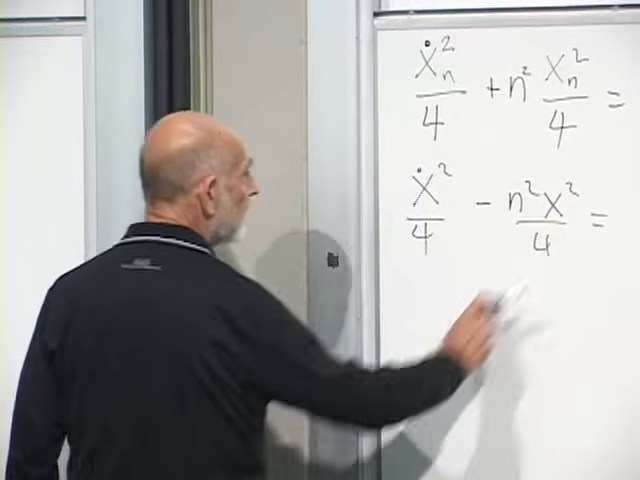
\includegraphics[width=0.82\textwidth]{lecture_03_figure_02.png}\caption{Le calcul au tableau, où le commutateur canonique fournit le facteur \(n\).}\lectureframe{00:10:30}\label{fig:l03-commutator-board}\end{figure}

Le facteur \(n\) nous indique comment normaliser les opérateurs d’échelle :

\begin{align}
  a_n
  &\equiv
  \frac{\sqrt n}{2}X_n+\frac{i}{\sqrt n}p_n,
  \label{eq:l03-annihilator}\\
  a_n^\dagger
  &\equiv
  \frac{\sqrt n}{2}X_n-\frac{i}{\sqrt n}p_n.
  \label{eq:l03-creator}
\end{align}

Ils vérifient

\begin{equation}
  [a_n,a_m^\dagger]=\delta_{nm},
  \qquad
  H_n=n\left(a_n^\dagger a_n+\frac12\right).
  \label{eq:l03-oscillator-algebra}
\end{equation}

Ainsi, \(a_n^\dagger\) ajoute un quantum au \(n\)e oscillateur, mais ce quantum porte une énergie de mode de \(n\) unités. L’espacement familier de l’oscillateur n’a pas disparu ; sa fréquence est \(\omega_n=n\).

\begin{figure}[H]\centering
  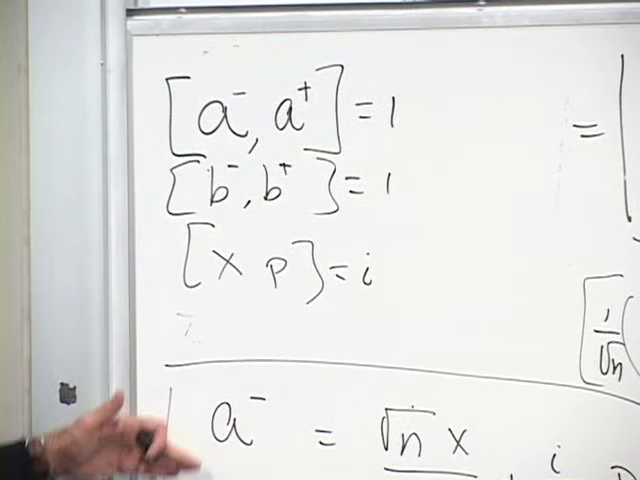
\includegraphics[width=0.82\textwidth]{lecture_03_figure_03.png}\caption{Opérateurs d’annihilation et de création normalisés pour le \(n\)e oscillateur de la corde.}\lectureframe{00:12:00}\label{fig:l03-ladder-board}\end{figure}

\subsection{Deux tours transverses}

Dans un espace-temps à quatre dimensions, une corde portant une très grande quantité de mouvement selon l’axe \(z\) a deux coordonnées transverses, \(X\) et \(Y\). Il nous faut donc deux tours d’oscillateurs indépendants. Notons \(a_n,a_n^\dagger\) les opérateurs agissant sur les modes \(X\) et \(b_n,b_n^\dagger\) ceux qui agissent sur les modes \(Y\). Résoudre \eqref{eq:l03-annihilator}--\eqref{eq:l03-creator} par rapport aux coordonnées donne

\begin{equation}
  X_n=\frac{a_n+a_n^\dagger}{\sqrt n},
  \qquad
  Y_n=\frac{b_n+b_n^\dagger}{\sqrt n}.
  \label{eq:l03-mode-coordinates}
\end{equation}

\begin{figure}[H]\centering
  \includegraphics[width=0.78\textwidth]{lecture_03_figure_04.png}\caption{Résolution de la coordonnée d’un mode en fonction de ses opérateurs de création et d’annihilation.}\lectureframe{00:17:05}\label{fig:l03-coordinate-operator-board}\end{figure}

Les coordonnées de la corde ouverte ont été développées en modes de Neumann,

\begin{align}
  X(\sigma,\tau)
  &=X_{\rm cm}(\tau)
    +\sum_{n=1}^{\infty}X_n(\tau)\cos(n\sigma),
  \label{eq:l03-X-fourier}\\
  Y(\sigma,\tau)
  &=Y_{\rm cm}(\tau)
    +\sum_{n=1}^{\infty}Y_n(\tau)\cos(n\sigma).
  \label{eq:l03-Y-fourier}
\end{align}

Les cosinus apparaissent parce que les pentes aux extrémités s’annulent. En substituant \eqref{eq:l03-mode-coordinates}, on transforme la corde elle-même en opérateur :

\begin{align}
  X(\sigma,\tau)
  &=X_{\rm cm}(\tau)
    +\sum_{n=1}^{\infty}
      \frac{a_n(\tau)+a_n^\dagger(\tau)}{\sqrt n}
      \cos(n\sigma),
  \label{eq:l03-X-operator}\\
  Y(\sigma,\tau)
  &=Y_{\rm cm}(\tau)
    +\sum_{n=1}^{\infty}
      \frac{b_n(\tau)+b_n^\dagger(\tau)}{\sqrt n}
      \cos(n\sigma).
  \label{eq:l03-Y-operator}
\end{align}

\begin{figure}[H]\centering
  \begin{minipage}[t]{0.48\textwidth}\centering
    \includegraphics[width=\textwidth]{lecture_03_figure_05.png}\par\smallskip\footnotesize (a) Développements en modes des coordonnées. \end{minipage}\hfill
  \begin{minipage}[t]{0.48\textwidth}\centering
    \includegraphics[width=\textwidth]{lecture_03_figure_06.png}\par\smallskip\footnotesize (b) Opérateurs d’échelle substitués dans les coordonnées de la corde.\end{minipage}\caption{La forme de la corde ouverte quantique est assemblée à partir de tous ses opérateurs d’oscillateurs transverses.}\lectureframe{00:20:35 and 00:21:05}\label{fig:l03-string-coordinate-board}\end{figure}

\begin{classroomqa}\audiencequestion{\(X_n\) est-il également fonction de \(\sigma\) ?\lecturetimestamp{00:21:48}}\lecturerresponse{Non. La dépendance en \(\sigma\) se trouve entièrement dans \(\cos(n\sigma)\). Le coefficient \(X_n\) est l’amplitude, dépendante du temps, de ce profil spatial ; ainsi, \(X_n=X_n(\tau)\).}\end{classroomqa}

\begin{classroomqa}\audiencequestion{Pourquoi les opérateurs appelés opérateurs de montée et de descente semblent-ils avoir leurs signes inversés ?\lecturetimestamp{00:23:13}}\lecturerresponse{Le signe visible de \(ip_n\) ne détermine pas le nom de l’opérateur. Calculons le commutateur avec le hamiltonien. L’opérateur qui vérifie \([H_n,a_n^\dagger]=n a_n^\dagger\) augmente l’énergie ; celui qui vérifie \([H_n,a_n]=-n a_n\) la diminue.}\end{classroomqa}

Les deux tours transverses constituent une représentation pédagogique en quatre dimensions. Une corde bosonique quantifiée de façon cohérente possède vingt-six dimensions d’espace-temps ; elle a donc vingt-quatre familles d’oscillateurs transverses, au lieu de deux. Le raisonnement qui suit reste le même : le nombre d’états du premier niveau doit correspondre au nombre de polarisations physiques d’un vecteur sans masse dans la même dimension.

\section{Spin massif et hélicité sans masse}

Avant d’attribuer un spin aux états de la corde, il faut établir une distinction nette. Une particule massive de spin \(J\) possède \(2J+1\) états de spin,

\begin{equation}
  m_J=-J,-J+1,\ldots,J-1,J.
  \label{eq:l03-massive-spin-multiplet}
\end{equation}

Par exemple, une particule massive de spin un possède trois polarisations et une particule massive de spin deux en possède cinq. On comprend pourquoi en se plaçant dans le référentiel au repos. Toutes les rotations spatiales y sont possibles. On fait tourner l’axe de spin, puis on effectue un boost en retour ; les \(2J+1\) composantes appartiennent alors toutes à la même particule relativiste.

Une particule sans masse n’a pas de référentiel au repos. Son étiquette de spin invariante est l’hélicité, c’est-à-dire le moment cinétique selon sa direction de mouvement. Un photon n’a que les hélicités \(h=+1\) et \(h=-1\) ; un graviton n’a que \(h=+2\) et \(h=-2\). Un scalaire n’a qu’un état \(h=0\). Le cours utilise la symétrie par réflexion pour associer les deux hélicités. Dans une théorie chirale, une représentation irréductible sans masse peut ne porter qu’une seule hélicité ; l’association des deux est donc une affirmation de symétrie supplémentaire, et non une conséquence de la seule absence de masse.\editorialnote{La classification moderne par le groupe petit admet des représentations sans masse à une seule hélicité. La parité ou un contenu de champs approprié, complété par CPT, fournit l’hélicité opposée dans les exemples familiers du photon et du graviton.}

\begin{figure}[H]\centering
  \begin{minipage}[t]{0.45\textwidth}\centering
    \includegraphics[width=\textwidth]{lecture_03_figure_07.png}\par\smallskip\footnotesize (a) Le décompte des états de spin commencé au tableau. \end{minipage}\hfill
  \begin{minipage}[t]{0.5\textwidth}\centering
    \begin{adjustbox}{max width=\linewidth}\begin{tabular}{@{}ccc@{}}\toprule
      Spin & États massifs & Hélicités sans masse \\\midrule
      \(0\)&\(1\)&\(0\)\\\(1\)&\(3\)&\(+1,-1\)\\\(2\)&\(5\)&\(+2,-2\)\\\bottomrule
    \end{tabular}\end{adjustbox}\end{minipage}\caption{La masse élimine le référentiel au repos et, avec lui, les projections de spin intermédiaires.}\lectureframe{00:27:40}\label{fig:l03-spin-count}\end{figure}

\subsection{Polarisation linéaire et circulaire du photon}

Considérons un photon qui se déplace selon \(z\). Ses deux polarisations linéaires transverses sont \(\ket{x}\) et \(\ket{y}\). Elles ne sont pas des états propres de l’hélicité. Les états circulaires sont

\begin{align}
  \ket{R}
  &=\frac{1}{\sqrt2}\left(\ket{x}+i\ket{y}\right),
  \label{eq:l03-right-circular}\\
  \ket{L}
  &=\frac{1}{\sqrt2}\left(\ket{x}-i\ket{y}\right),
  \label{eq:l03-left-circular}
\end{align}

avec les hélicités \(+1\) et \(-1\), selon la convention adoptée pour nommer les polarisations droite et gauche. Un photon polarisé linéairement est une superposition de ces deux résultats possibles. Son hélicité moyenne peut être nulle, mais une mesure de l’hélicité ne donne jamais un photon de spin nul. De même,

\begin{equation}
  \frac{1}{\sqrt2}\left(\ket{x}+\ket{y}\right)
\end{equation}

correspond simplement à une polarisation linéaire à quarante-cinq degrés.

\begin{figure}[H]\centering
  \begin{minipage}[t]{0.48\textwidth}\centering
    \includegraphics[width=\textwidth]{lecture_03_figure_08.png}\par\smallskip\footnotesize (a) États de polarisation circulaire au tableau. \end{minipage}\hfill
  \begin{minipage}[t]{0.48\textwidth}\centering
    \begin{adjustbox}{max width=\linewidth}\begin{tikzpicture}[>=Latex,scale=0.9]
      \draw[->,thick] (0,0) -- (3.4,0) node[right] {\(z\)};
      \draw[->,blue!70!black,thick] (0,0) -- (0,2.0)
        node[above] {\(x\)};
      \draw[->,orange!85!black,thick] (0,0) -- (-1.4,-1.2)
        node[below left] {\(y\)};
      \draw[red!70!black,thick,->]
        plot[domain=0:320,samples=80]
        ({1.0*cos(\x)},{0.58*sin(\x)+0.4});
      \node[red!70!black] at (1.55,1.25) {circular};
    \end{tikzpicture}\end{adjustbox}\end{minipage}\caption{Une base transverse est fournie par la polarisation linéaire ; les combinaisons circulaires diagonalisent l’hélicité.}\lectureframe{00:37:45}\label{fig:l03-polarization}\end{figure}

\begin{classroomqa}\audiencequestion{Est-ce analogue à la séparation des états de spin dans une expérience de Stern--Gerlach ?\lecturetimestamp{00:37:40}}\lecturerresponse{L’idée de superposition quantique est la même, mais pour le photon, le langage direct est celui de la polarisation. Une mesure de la polarisation circulaire distingue les deux hélicités ; le faisceau ne contient pas de photon longitudinal de spin nul.}\end{classroomqa}

Le graviton reprend le même schéma avec le spin deux. Pour tenir compte des spins, on peut écrire schématiquement

\begin{equation}
  \ket{+2}\sim\ket{+1}\otimes\ket{+1},
  \qquad
  \ket{-2}\sim\ket{-1}\otimes\ket{-1}.
  \label{eq:l03-graviton-helicity}
\end{equation}

Cela ne signifie pas qu’un graviton est littéralement constitué de deux photons. Cela signifie que deux hélicités égales s’additionnent pour donner l’hélicité correcte de spin deux.

\begin{classroomqa}\audiencequestion{L’analogie avec deux photons s’étend-elle à d’autres nombres quantiques ?\lecturetimestamp{00:41:05}}\lecturerresponse{Pas comme modèle de constituants. Il existe des formules puissantes dans lesquelles les amplitudes gravitationnelles ressemblent à des produits, ou à des carrés``'', d’amplitudes de théorie de jauge, mais le graviton reste une particule à part entière. Ici, l’analogie est surtout fiable comme énoncé sur l’hélicité.\editorialnote{Les relations modernes de Kawai--Lewellen--Tye et de double copie précisent l’énoncé sur les amplitudes dans certaines théories ; elles ne font pas du graviton un état lié de deux photons.}}\end{classroomqa}

\begin{classroomqa}\audiencequestion{Un photon peut avoir n’importe quelle quantité de mouvement ; son spectre n’est-il donc pas continu, au lieu d’être discret comme l’exige celui d’une particule ?\lecturetimestamp{00:42:17}}\lecturerresponse{La variable continue est la quantité de mouvement du centre de masse. Fixons cette quantité de mouvement et examinons la masse invariante interne. Une particule est identifiée par un niveau de masse discret ; la variation de sa quantité de mouvement globale produit ensuite la relation de dispersion continue habituelle.}\end{classroomqa}

\section{Les niveaux les plus bas de la corde ouverte}

Nous pouvons maintenant revenir à la corde. Dans la description à grande quantité de mouvement, l’énergie interne finie de front lumineux est proportionnelle à la masse invariante au carré. En omettant le facteur global correspondant à l’échelle de la corde, écrivons le spectre sous la forme

\begin{equation}
  \begin{aligned}
    M^2
    &=m_0^2
      +\sum_{n=1}^{\infty}n
       \left(N_n^{(a)}+N_n^{(b)}\right),\\
    N_n^{(a)}&=a_n^\dagger a_n,
    \qquad
    N_n^{(b)}=b_n^\dagger b_n.
  \end{aligned}
  \label{eq:l03-open-spectrum}
\end{equation}

L’état fondamental de l’oscillateur vérifie

\begin{equation}
  a_n\ket{0}=0,
  \qquad
  b_n\ket{0}=0,
  \qquad n=1,2,\ldots .
  \label{eq:l03-ground-annihilation}
\end{equation}

Ce n’est pas une absence de corde. C’est l’état quantique le moins excité de la corde, dont les coordonnées fluctuent toujours. Notons sa masse au carré \(m_0^2\), qu’il reste à déterminer.

\begin{figure}[H]\centering
  \includegraphics[width=0.78\textwidth]{lecture_03_figure_09.png}\caption{L’état fondamental de la corde ouverte et les conditions d’annihilation qui le définissent.}\lectureframe{00:45:20}\label{fig:l03-ground-state-board}\end{figure}

Les excitations les moins coûteuses font intervenir les opérateurs de création \(n=1\) :

\begin{equation}
  a_1^\dagger\ket{0},
  \qquad
  b_1^\dagger\ket{0},
  \qquad
  M^2=m_0^2+1.
  \label{eq:l03-first-level}
\end{equation}

\begin{figure}[H]\centering
  \includegraphics[width=0.78\textwidth]{lecture_03_figure_10.png}\caption{L’un des deux états dégénérés du premier niveau, avec l’incrément de masse au carré inscrit au tableau.}\lectureframe{00:49:25}\label{fig:l03-first-level-board}\end{figure}

Le mot ``un'' dans l’eqref{eq:l03-first-level} ne désigne pas un joule, un électronvolt ni une masse de Planck. Nous avons omis l’échelle dimensionnée de la corde. Pour l’instant, il signifie un échelon dans la tour des masses au carré de l’oscillateur ; les unités manquantes seront rétablies au cours suivant.

Toute combinaison linéaire des deux états dégénérés est également un état de ce niveau. En particulier,

\begin{equation}
  \frac{1}{\sqrt2}
  \left(a_1^\dagger\pm i b_1^\dagger\right)\ket{0}
  \label{eq:l03-string-circular-states}
\end{equation}

est l’analogue, pour la corde, de la polarisation circulaire. Sous une rotation dans le plan \(x\)-\(y\), \(a_1^\dagger\) et \(b_1^\dagger\) se transforment comme les deux composantes d’un vecteur transverse. Les combinaisons de \eqref{eq:l03-string-circular-states} ont donc les hélicités \(+1\) et \(-1\).

\begin{figure}[H]\centering
  \includegraphics[width=0.82\textwidth]{lecture_03_figure_11.png}\caption{Conditions de l’état fondamental, deux excitations du premier niveau et leurs combinaisons circulaires, réunies au tableau.}\lectureframe{00:56:00}\label{fig:l03-level-structure-board}\end{figure}

Il n’existe pas de troisième état dégénéré qui puisse servir de polarisation longitudinale. Si ces deux états avaient une masse non nulle, une particule relativiste de spin un exigerait trois polarisations. Avec exactement deux polarisations, l’état doit donc être sans masse. Ainsi,

\begin{equation}
  m_0^2+1=0,
  \qquad
  m_0^2=-1.
  \label{eq:l03-intercept-condition}
\end{equation}

Le premier niveau ressemble à celui du photon : c’est un état de vecteur de jauge sans masse. Il ne s’agit pas nécessairement du photon de l’électromagnétisme ; son identité de jauge éventuelle dépend du modèle de corde. L’état fondamental qui lui est inférieur a une masse au carré négative. C’est le tachyon de la corde bosonique ouverte.\editorialnote{Dans la corde bosonique critique complète, l’intercept de l’ordre normal et l’algèbre de Lorentz sont liés à \(D=26\). Le calcul du cours avec deux directions transverses est la projection en quatre dimensions du même argument de dénombrement des états : les états d’oscillateur du premier niveau, au nombre de \(D-2\), correspondent aux polarisations physiques d’un vecteur sans masse, au nombre de \(D-2\).}

\begin{classroomqa}\audiencequestion{Pourquoi faut-il s’intéresser au fait que \(m_0^2\) est négative ?\lecturetimestamp{00:56:35}}\lecturerresponse{Parce que la masse au carré est la courbure du potentiel quadratique du champ autour de l’état que nous avons appelé le vide. Une courbure négative signifie que cette configuration n’est pas un état fondamental stable. Le calcul suivant rend cette affirmation précise.}\end{classroomqa}

\section{Ce que signifie réellement un tachyon}

Le nom ``tachyon'' suggère d’abord une idée trompeuse. Partons de la relation de dispersion relativiste avec \(c=1\),

\begin{equation}
  E(p)=\sqrt{p^2+m^2}.
  \label{eq:l03-relativistic-dispersion}
\end{equation}

Pour un paquet d’ondes, la vitesse de groupe est

\begin{equation}
  v_g=\frac{dE}{dp}.
  \label{eq:l03-group-velocity}
\end{equation}

On retrouve ainsi des cas familiers :

\begin{align}
  E_{\rm nr}(p)&=\frac{p^2}{2m},
  &v_g&=\frac{p}{m},
  \label{eq:l03-nr-group-velocity}\\
  E_\gamma(p)&=|p|,
  &|v_g|&=1,
  \label{eq:l03-photon-group-velocity}\\
  E_m(p)&=\sqrt{p^2+m^2},
  &|v_g|&=\frac{|p|}{\sqrt{p^2+m^2}}<1.
  \label{eq:l03-massive-group-velocity}
\end{align}

\begin{figure}[H]\centering
  \begin{minipage}[t]{0.48\textwidth}\centering
    \includegraphics[width=\textwidth]{lecture_03_figure_12.png}\par\smallskip\footnotesize (a) Vitesse de groupe non relativiste. \end{minipage}\hfill
  \begin{minipage}[t]{0.48\textwidth}\centering
    \includegraphics[width=\textwidth]{lecture_03_figure_13.png}\par\smallskip\footnotesize (b) Relation de dispersion relativiste et sa dérivée.\end{minipage}\caption{Lire la vitesse de propagation sur la pente de \(E(p)\).}\lectureframe{01:01:50 and 01:03:15}\label{fig:l03-group-velocity-board}\end{figure}

Si \(m^2=-\mu^2\), l’expression formelle devient

\begin{equation}
  E(p)=\sqrt{p^2-\mu^2},
  \qquad
  v_g=\frac{p}{\sqrt{p^2-\mu^2}},
  \label{eq:l03-formal-tachyon-dispersion}
\end{equation}

qui vérifie \(|v_g|>1\) chaque fois que la racine carrée est réelle. Mais ce n’est pas la bonne interprétation physique de l’état fondamental de la corde bosonique. Le problème apparaît déjà à faible quantité de mouvement, où la fréquence est imaginaire.

\subsection{Courbure négative du potentiel du champ}

Considérons un champ scalaire réel en une dimension spatiale,

\begin{equation}
  \left(\partial_t^2-\partial_x^2+m^2\right)\phi=0.
  \label{eq:l03-klein-gordon}
\end{equation}

Pour une onde plane \(\phi\propto e^{-i\omega t+ikx}\),

\begin{equation}
  \omega^2=k^2+m^2.
  \label{eq:l03-kg-dispersion}
\end{equation}

\begin{figure}[H]\centering
  \includegraphics[width=0.82\textwidth]{lecture_03_figure_14.png}\caption{L’équation de Klein--Gordon utilisée pour mettre en évidence l’instabilité associée à une masse au carré négative.}\lectureframe{01:06:40}\label{fig:l03-klein-gordon-board}\end{figure}

L’énergie quadratique conservée est

\begin{equation}
  \mathcal E
  =\frac12\int dx\,
  \left[
    \dot\phi^{\,2}
    +(\partial_x\phi)^2
    +m^2\phi^2
  \right].
  \label{eq:l03-field-energy}
\end{equation}

\begin{figure}[H]\centering
  \includegraphics[width=0.82\textwidth]{lecture_03_figure_15.png}\caption{Énergie du champ scalaire, dont le terme de masse donne la courbure locale du potentiel.}\lectureframe{01:08:10}\label{fig:l03-field-energy-board}\end{figure}

Pour \(m^2>0\), le potentiel local \(V(\phi)=\tfrac12m^2\phi^2\) a la forme d’une cuvette. La configuration \(\phi=0\) se trouve au fond. Pour \(m^2=-\mu^2\), le même point est au sommet d’une cuvette inversée. L’équation \eqref{eq:l03-kg-dispersion} devient

\begin{equation}
  \omega^2=k^2-\mu^2.
  \label{eq:l03-tachyonic-modes}
\end{equation}

Les modes tels que \(k^2<\mu^2\) ont

\begin{equation}
  \omega=\pm i\sqrt{\mu^2-k^2},
  \qquad
  \phi_k(t)\propto
  e^{\pm\sqrt{\mu^2-k^2}\,t}.
  \label{eq:l03-growing-mode}
\end{equation}

Une branche croît exponentiellement. Le prétendu vide est donc instable : une perturbation de grande longueur d’onde, aussi petite soit-elle, éloigne le champ de \(\phi=0\). Voilà ce que signifie la présence d’un tachyon dans le spectre.

\subsection{La chaîne de pendules en équilibre instable}

Une rangée de pendules couplés rend cette distinction visible. Plaçons tous les pendules à la verticale, en équilibre inversé. La configuration uniforme existe, mais elle est en équilibre au maximum de l’énergie potentielle. On donne une légère impulsion à un pendule ; il tombe et entraîne ses voisins. Un front de chute se propage le long de la chaîne à la vitesse de signal finie imposée par les couplages.

\begin{figure}[H]\centering
  \begin{minipage}[t]{0.48\textwidth}\centering
    \includegraphics[width=\textwidth]{lecture_03_figure_16.png}\par\smallskip\footnotesize (a) Le modèle de pendules couplés en équilibre inversé, au tableau. \end{minipage}\hfill
  \begin{minipage}[t]{0.48\textwidth}\centering
    \begin{adjustbox}{max width=\linewidth}\begin{tikzpicture}[>=Latex,scale=0.78]
      \draw[thick] (-0.3,0) -- (6.3,0);
      \foreach \x/\a in {0/0,1/0,2/8,3/28,4/55,5/72,6/78}{
        \fill (\x,0) circle (0.06);
        \draw[thick] (\x,0) -- ++({90-\a}:1.25);
        \fill[blue!65!black]
          ($(\x,0)+({90-\a}:1.25)$) circle (0.11);
      }
      \draw[red!70!black,->,thick] (1.7,-0.45) -- (4.6,-0.45)
        node[midway,below] {falling front};
    \end{tikzpicture}\end{adjustbox}\end{minipage}\caption{L’instabilité se propage de façon causale dans un système, même si son spectre linéarisé contient une masse au carré négative.}\lectureframe{01:10:40}\label{fig:l03-pendulum-instability}\end{figure}

Rien dans ce mécanisme ne permet à un signal contrôlé de dépasser le front causal. Un mode tachyonique signale un point de développement inapproprié, et non un messager supraluminique stable.\editorialnote{Pour une équation de champ relativiste locale, la vitesse de front reste la vitesse causale. La vitesse de groupe formelle de la branche réelle à grande \(k\) ne transforme pas le vide instable en canal de communication supraluminique.}

\begin{classroomqa}\audiencequestion{L’état sans masse que nous venons de trouver est-il le graviton prédit par la théorie des cordes ?\lecturetimestamp{01:14:27}}\lecturerresponse{Non. C’est l’état de spin un d’une corde ouverte, à deux polarisations ; il ressemble donc à un boson de jauge. Le graviton est une excitation de spin deux d’une corde fermée.}\end{classroomqa}

\begin{classroomqa}\audiencequestion{Un potentiel inversé est-il mathématiquement admissible et où le système aboutirait-il après sa chute ?\lecturetimestamp{01:15:17}}\lecturerresponse{C’est une approximation locale tout à fait légitime, mais elle ne possède pas à elle seule d’état fondamental, car l’énergie n’est pas bornée inférieurement. Un potentiel plus complet peut se recourber vers le haut et posséder un minimum plus bas. Le système évolue alors en roulant ou en se condensant vers cette configuration stable.}\end{classroomqa}

La corde bosonique ordinaire présente précisément ce défaut. Ses états d’oscillateur de plus haute énergie restent dans le spectre, mais ce sont des excitations d’un arrière-plan instable. Les théories cohérentes de supercordes éliminent le tachyon de la corde ouverte dans leurs secteurs stables tout en conservant les excitations de corde sans masse et massives.

\begin{classroomqa}\audiencequestion{Les autres propriétés de l’état de la corde ouverte correspondent-elles aussi à celles d’un photon, comme le font ses deux polarisations ?\lecturetimestamp{01:17:07}}\lecturerresponse{Cet état se comporte comme un boson de jauge sans masse. Ses affectations de charges, ses règles de rayonnement et son identité détaillées dépendent du modèle de corde ; il vaut donc mieux le qualifier de semblable à un photon plutôt que de l’identifier d’emblée à l’électromagnétisme. Ces propriétés d’interaction seront étudiées plus loin.}\end{classroomqa}

\section{Interactions entre cordes}

Le spectre libre ne représente que la moitié de la théorie. Les cordes se joignent et se scindent également. Il est utile de rappeler d’abord qu’une corde libre excitée peut porter un moment cinétique. Une corde droite en rotation tourne autour de son centre de masse, et son énergie et son moment cinétique augmentent ensemble le long de la trajectoire familière des cordes.

\begin{figure}[H]\centering
  \includegraphics[width=0.72\textwidth]{lecture_03_figure_17.png}\caption{Schéma d’une corde ouverte en rotation autour de son centre de masse.}\lectureframe{01:19:30}\label{fig:l03-rotating-string-board}\end{figure}

\begin{classroomqa}\audiencequestion{Une corde libre peut-elle tourner bout à bout autour d’une seule extrémité fixe ?\lecturetimestamp{01:20:02}}\lecturerresponse{Pas sans point d’ancrage. Un système libre et isolé tourne autour de son centre de masse. Si une extrémité est attachée à un autre objet ou à une brane, le système combiné peut tourner autour d’un autre centre, comme un électron et un noyau qui orbitent autour de leur centre de masse commun tandis que le noyau, beaucoup plus lourd, semble presque immobile.}\end{classroomqa}

\subsection{Le vertex de la corde ouverte}

Pour les cordes ouvertes, l’interaction élémentaire a lieu lorsque deux extrémités se rencontrent au même point de l’espace-temps. Il existe une amplitude \(g_s\) pour qu’elles se joignent et forment une seule corde. L’histoire inverse donne une amplitude pour qu’une corde se scinde en deux. Schématiquement,

\begin{equation}
  \text{open}+\text{open}
  \quad\rightleftarrows\quad
  \text{open}.
  \label{eq:l03-open-joining}
\end{equation}

\begin{figure}[H]\centering
  \begin{minipage}[t]{0.48\textwidth}\centering
    \includegraphics[width=\textwidth]{lecture_03_figure_18.png}\par\smallskip\footnotesize (a) Le processus de jonction représenté au tableau. \end{minipage}\hfill
  \begin{minipage}[t]{0.48\textwidth}\centering
    \begin{tikzpicture}[>=Latex,scale=0.9]
      \draw[->] (0,-2.1) -- (0,2.2) node[above] {time};
      \draw[blue!70!black,thick] (-2,-1.6) .. controls (-1.3,-0.9)
        and (-0.7,-0.35) .. (0,0);
      \draw[blue!70!black,thick] (2,-1.6) .. controls (1.3,-0.9)
        and (0.7,-0.35) .. (0,0);
      \draw[orange!85!black,thick] (0,0) .. controls (0.25,0.7)
        and (-0.15,1.25) .. (0.15,1.9);
      \fill[red!70!black] (0,0) circle (0.09);
      \node[right] at (0.12,0) {\(g_s\)};
    \end{tikzpicture}\end{minipage}\caption{La jonction des extrémités est l’analogue, pour les cordes, d’un vertex d’interaction locale entre particules ; l’inversion du temps donne la scission.}\lectureframe{01:24:05}\label{fig:l03-open-vertex}\end{figure}

Le couplage est une amplitude. Pour un processus élémentaire donné, la probabilité correspondante commence à l’ordre \(|g_s|^2\), les facteurs d’espace des phases et de normalisation étant fournis par le calcul complet. Qualifier \(g_s\) de ``probabilité'' est donc un raccourci informel ; distinguer amplitude et probabilité évite de faire apparaître un carré injustifié.

L’interaction ne dépend pas du fait que la corde externe vibre, tourne ou se trouve dans un autre état d’oscillateur. Ces états modifient l’élément de matrice détaillé, mais la même règle locale de jonction s’applique.

\subsection{Une corde ouverte peut se refermer sur elle-même}

Supposons que les deux extrémités d’une corde ouverte se rencontrent. La règle de jonction ne peut pas savoir qu’elles appartiennent à la même corde. Elles peuvent fusionner et produire une boucle fermée :

\begin{equation}
  \text{open}\longrightarrow\text{closed}.
  \label{eq:l03-self-closing}
\end{equation}

\begin{figure}[H]\centering
  \begin{minipage}[t]{0.48\textwidth}\centering
    \includegraphics[width=\textwidth]{lecture_03_figure_19.png}\par\smallskip\footnotesize (a) La corde ouverte rapproche ses extrémités. \end{minipage}\hfill
  \begin{minipage}[t]{0.48\textwidth}\centering
    \begin{tikzpicture}[>=Latex,scale=0.92]
      \draw[blue!70!black,thick]
        (-2,0) .. controls (-1.2,1.5) and (1.2,1.5) .. (2,0);
      \fill[red!70!black] (-2,0) circle (0.08);
      \fill[red!70!black] (2,0) circle (0.08);
      \draw[->,thick] (-0.45,-0.45) -- (0.45,-0.45);
      \draw[orange!85!black,thick] (0,-1.55) ellipse (1.15 and 0.58);
      \node at (0,-2.25) {closed string};
    \end{tikzpicture}\end{minipage}\caption{Les interactions entre cordes ouvertes engendrent inévitablement des cordes fermées.}\lectureframe{01:27:20}\label{fig:l03-open-becomes-closed}\end{figure}

Ce n’est pas un ajout facultatif. Toute théorie de cordes ouvertes en interaction doit contenir des états de cordes fermées. Le processus inverse permet à une corde fermée de s’ouvrir en une corde ouverte, lorsque les extrémités admissibles et les conditions aux limites le permettent.

\begin{classroomqa}\audiencequestion{Lorsque les cordes fusionnent ou se scindent, leur énergie d’oscillation change-t-elle, et la théorie détermine-t-elle comment ?\lecturetimestamp{01:28:05}}\lecturerresponse{Oui. L’énergie et la quantité de mouvement se conservent dans le processus complet, tandis que l’excitation peut se redistribuer entre les cordes qui en résultent. Le vertex d’interaction et les fonctions d’onde externes déterminent l’amplitude de transition.}\end{classroomqa}

\subsection{Les cordes fermées peuvent interagir sans s’ouvrir}

L’implication ne vaut que dans un sens. Les cordes ouvertes en interaction exigent des cordes fermées, mais une théorie peut ne contenir au départ que des cordes fermées. Deux boucles fermées peuvent se toucher, se reconnecter et n’en former qu’une seule ; le processus inverse scinde une boucle en deux. Aucune extrémité ouverte n’a besoin d’apparaître.

\begin{figure}[H]\centering
  \begin{minipage}[t]{0.48\textwidth}\centering
    \includegraphics[width=\textwidth]{lecture_03_figure_20.png}\par\smallskip\footnotesize (a) Fusion de cordes fermées au tableau. \end{minipage}\hfill
  \begin{minipage}[t]{0.48\textwidth}\centering
    \begin{tikzpicture}[>=Latex,scale=0.88]
      \draw[blue!70!black,thick] (-1.35,0) circle (0.75);
      \draw[blue!70!black,thick] (1.35,0) circle (0.75);
      \draw[->,thick] (-0.35,-1.15) -- (0.35,-1.15);
      \draw[orange!85!black,thick] (0,-2.3) ellipse (1.35 and 0.68);
      \node at (0,1.2) {closed \(+\) closed};
      \node at (0,-3.25) {closed};
    \end{tikzpicture}\end{minipage}\caption{Les cordes fermées possèdent leur propre interaction de jonction et de scission et n’ont pas à passer par un état de corde ouverte.}\lectureframe{01:29:05}\label{fig:l03-closed-fusion}\end{figure}

\begin{classroomqa}\audiencequestion{Une théorie qui commence par des cordes fermées doit-elle aussi contenir des cordes ouvertes ?\lecturetimestamp{01:28:35}}\lecturerresponse{Non. Les cordes fermées peuvent interagir par reconnexion tout en restant fermées. Les cordes ouvertes requièrent des données de bord supplémentaires, comme des extrémités admissibles ou des branes.}\end{classroomqa}

\section{Pourquoi la gravité est inévitable}

Le calcul des oscillateurs d’une corde fermée est parallèle à celui d’une corde ouverte, mais il y a des excitations indépendantes se déplaçant vers la gauche et vers la droite. Leur premier niveau non trivial apparié contient un état sans masse de spin deux. Cet état possède les hélicités d’un graviton. Par conséquent, toute théorie cohérente de cordes fermées en interaction contient la gravité.

\begin{classroomqa}\audiencequestion{Pourquoi l’excitation de plus basse énergie d’une corde fermée doit-elle être un graviton, tout comme le niveau de la corde ouverte devait ressembler à un photon ?\lecturetimestamp{01:30:59}}\lecturerresponse{La réponse repose sur le même type de dénombrement des états, cette fois avec les vecteurs d’oscillateur se déplaçant vers la gauche et vers la droite. Leur produit tensoriel contient une polarisation de spin deux sans masse, symétrique et sans trace. Le spectre explicite des cordes fermées sera établi au cours suivant ; à ce stade, le point essentiel est le caractère inévitable de cet état.}\end{classroomqa}

Les cordes ouvertes et fermées peuvent aussi interagir entre elles. Une boucle fermée peut rencontrer une corde ouverte et être absorbée, laissant une corde ouverte plus grande ou excitée différemment. Inversement, une corde ouverte peut émettre une boucle fermée. Au niveau des particules, cela correspond à l’émission ou à l’absorption d’un graviton par la matière.

\begin{figure}[H]\centering
  \begin{minipage}[t]{0.48\textwidth}\centering
    \includegraphics[width=\textwidth]{lecture_03_figure_21.png}\par\smallskip\footnotesize (a) Reconnexion locale de segments de corde. \end{minipage}\hfill
  \begin{minipage}[t]{0.48\textwidth}\centering
    \includegraphics[width=\textwidth]{lecture_03_figure_22.png}\par\smallskip\footnotesize (b) Une boucle fermée se rattache à une corde ouverte. \end{minipage}\caption{Les schémas au tableau illustrant les interactions mixtes entre cordes ouvertes--et fermées, ainsi que la possibilité universelle d’échange d’un graviton.}\lectureframe{01:33:10 and 01:34:35}\label{fig:l03-mixed-interactions-board}\end{figure}

\begin{figure}[H]\centering
  \begin{tikzpicture}[>=Latex,scale=0.88]
    \draw[blue!70!black,thick]
      (-3,-0.5) .. controls (-1.7,-0.1) and (-0.8,0.2) .. (0,0);
    \draw[blue!70!black,thick]
      (0,0) .. controls (0.9,0.3) and (2.0,0.1) .. (3,0.55);
    \draw[orange!85!black,thick] (-0.8,1.55) ellipse (0.75 and 0.45);
    \draw[->,red!70!black,thick] (-0.45,1.15) -- (-0.05,0.35);
    \node[blue!70!black] at (-2.2,-0.95) {open string};
    \node[orange!85!black] at (-0.8,2.25) {closed string};
    \node at (1.75,-0.5) {excited open string};
  \end{tikzpicture}\caption{Schéma épuré, sans espace-temps, de l’absorption d’une corde fermée par une corde ouverte.}\label{fig:l03-mixed-interaction-redraw}\end{figure}

Le graviton peut se coupler à chaque état de corde, car toute corde porte de l’énergie et de la quantité de mouvement, et les règles de jonction autorisent l’échange de cordes fermées. C’est ainsi que la théorie des cordes rend compte de l’universalité de la gravité.

\begin{classroomqa}\audiencequestion{Une corde fermée peut-elle devenir une corde ouverte, ou se joindre à une corde ouverte sans enfreindre la règle sur les extrémités ?\lecturetimestamp{01:31:20}}\lecturerresponse{Dans une théorie qui contient les deux secteurs, une corde fermée peut se rattacher à une corde ouverte et modifier son état. La possibilité qu’une corde fermée isolée s’ouvre simplement dépend de la présence, dans la théorie, d’extrémités admissibles. La règle locale de reconnexion reste la même.}\end{classroomqa}

\begin{classroomqa}
\audiencequestion{Des boucles fermées peuvent-elles rester liées ou nouées de façon permanente ?\lecturetimestamp{01:35:10}}
\lecturerresponse{À faible couplage, les cordes sont presque transparentes : elles peuvent se traverser, sauf si la faible amplitude de reconnexion intervient. Un lien ou un nœud peut donc persister quelque temps, mais la topologie peut changer lorsqu’une interaction entre cordes autorisée se produit.}
\end{classroomqa}

\begin{classroomqa}
\audiencequestion{La probabilité d’interaction est-elle indépendante de l’état ou de la vitesse de la corde ?\lecturetimestamp{01:36:09}}
\lecturerresponse{Le couplage local est le même paramètre, mais la probabilité totale de transition dépend aussi des fonctions d’onde et de la durée pendant laquelle les portions concernées restent en contact. Une rencontre rapide laisse généralement moins de temps à l’interaction qu’une rencontre lente.}
\end{classroomqa}

\section{L’échelle et le couplage qui manquent encore}

Deux éléments du bilan dimensionnel ont été délibérément laissés de côté. Premièrement, \(X\) est une longueur, tandis que \(a_n\) est sans dimension ; la relation de proportionnalité dans \eqref{eq:l03-mode-coordinates} doit donc faire intervenir une échelle de longueur. Deuxièmement, augmenter le niveau de l’oscillateur ne peut pas littéralement ajouter un nombre sans dimension à une masse au carré physique. Rétablir la longueur de corde \(\ell_s\), ou, de façon équivalente, la pente de Regge \(\alpha'\sim\ell_s^2\), fournit les dimensions manquantes :

\begin{equation}
  M^2\sim\frac{1}{\alpha'}(N-a).
  \label{eq:l03-dimensional-spectrum}
\end{equation}

La convention précise et la normalisation seront fixées au prochain cours.

\begin{classroomqa}
\audiencequestion{Qu’est-ce qui fixe l’unité de longueur de la corde et la masse apportée par un opérateur de création ?\lecturetimestamp{01:37:03}}
\lecturerresponse{Une constante dimensionnée a été omise. Il s’agit de l’échelle de corde, généralement notée \(\ell_s\) ou \(\alpha'\). Les opérateurs d’oscillateur sont sans dimension ; les puissances de cette échelle convertissent leur nombre quantique en longueur, tension et masse au carré physiques.}
\end{classroomqa}

Le second paramètre est le couplage de corde \(g_s\). Dans la discussion la plus simple, il s’agit d’un nombre universel qui gouverne les processus de réunion et de séparation. Dans des modèles plus riches, les extrémités peuvent porter des étiquettes différentes et les cordes peuvent se rencontrer en des jonctions. Une configuration en Y est l’analogue, pour les cordes, de trois tubes de flux qui se rejoignent ; dans l’ancien modèle hadronique, elle est associée à un baryon composé de trois quarks, tandis qu’un unique segment ouvert ressemble à un méson composé d’un quark--antiquark.

\begin{classroomqa}
\audiencequestion{Des extrémités différentes d’une corde peuvent-elles avoir des probabilités de réunion différentes ?\lecturetimestamp{01:39:31}}
\lecturerresponse{Le modèle le plus simple utilise un seul couplage. Des théories plus élaborées attribuent des charges ou des étiquettes de bord aux extrémités ; des règles de sélection déterminent alors quelles réunions sont autorisées. La construction détaillée sera présentée plus tard, mais l’idée d’une réunion locale universelle demeure.}
\end{classroomqa}

\begin{classroomqa}
\audiencequestion{Une corde peut-elle se scinder dans le sens de la longueur ou former une jonction en Y ?\lecturetimestamp{01:40:01}}
\lecturerresponse{Certains systèmes de cordes admettent effectivement des jonctions. Il ne s’agit pas du processus ordinaire de séparation en deux extrémités qui vient d’être représenté ; elles apparaissent lorsque la théorie comporte des charges de corde compatibles. L’analogie des tubes de flux du méson--baryon aide à comprendre cette distinction.}
\end{classroomqa}

\begin{classroomqa}
\audiencequestion{Le changement du nombre de dimensions de l’espace-temps modifie-t-il le couplage d’interaction ?\lecturetimestamp{01:42:25}}
\lecturerresponse{Les dimensions modifient le spectre, l’espace des phases et les couplages effectifs obtenus après compactification. Le couplage fondamental de corde organise toujours le développement perturbatif, mais son expression en dimension inférieure dépend de la géométrie et du volume des dimensions supplémentaires.}
\end{classroomqa}

\begin{classroomqa}
\audiencequestion{Est-ce la gravité qui fait bouger une corde libre au départ ?\lecturetimestamp{01:43:17}}
\lecturerresponse{Aucune force n’est nécessaire pour entretenir le mouvement. La position et la vitesse initiales définissent une solution libre ; l’inertie la prolonge. La gravité ou une autre force modifie ce mouvement. La question de l’origine des conditions initiales est distincte et ne fait pas partie de l’équation locale du mouvement.}
\end{classroomqa}

Nous sommes donc parvenus à trois conclusions liées. La quantification d’une corde ouverte produit un vecteur sans masse à son premier niveau excité ; l’état fondamental bosonique situé en dessous est instable ; et les interactions introduisent inévitablement des cordes fermées, dont le spectre contient la gravité. Il reste à rétablir l’échelle manquante et à effectuer explicitement la quantification de la corde fermée.
\chapter{Cordes fermées, condition d’appariement des niveaux et dualité}

\lectureoverview{Une corde fermée porte des ondes indépendantes dans ses deux directions intrinsèques. La quantification de ces ondes semble d’abord doubler le photon de la corde ouverte, mais l’invariance par translation de l’origine de la coordonnée de la corde élimine les états qui ne se propagent que dans un seul sens. Le premier niveau qui subsiste contient une particule sans masse de spin 2. La même idée de changement de description ouvre alors une question plus vaste : lorsque les couplages varient, qu’est-ce qui fait d’un objet un constituant fondamental ?}

\section{Un générateur en réserve}

Avant de dessiner une corde fermée, retrouvons un résultat de mécanique analytique. Supposons que
\begin{equation}
  L=L(q_i,\dot q_i),
\end{equation}
et définissons le moment conjugué à \(q_i\) par
\begin{equation}
  p_i=\frac{\partial L}{\partial\dot q_i}.
\end{equation}
Une transformation continue infinitésimale s’écrit
\begin{equation}
  \delta q_i=\epsilon f_i(q),
  \label{eq:l04-infinitesimal-transformation}
\end{equation}
où \(\epsilon\) est un petit paramètre. Si cette transformation est une symétrie, le théorème de Noether fournit une charge conservée. Le déplacement de la coordonnée, rapporté au paramètre commun, donne le générateur
\begin{equation}
  Q=\sum_i p_i f_i(q)
   =\frac{1}{\epsilon}\sum_i p_i\,\delta q_i.
  \label{eq:l04-noether-charge}
\end{equation}
En mécanique quantique, \(Q\) est l’opérateur qui engendre la transformation infinitésimale correspondante.

Une rotation dans le plan \(xy\) en est l’exemple usuel. Pour un choix donné de l’orientation,
\begin{equation}
  \delta x=\epsilon y,
  \qquad
  \delta y=-\epsilon x,
\end{equation}
et \eqref{eq:l04-noether-charge} devient le moment cinétique, au signe près, qui dépend du même choix. Cet exemple précis importe peu. Ce qui compte, c’est le schéma : le moment conjugué contracté avec le déplacement infinitésimal donne le générateur.

\begin{figure}[H]
  \centering
  \includegraphics[width=0.76\textwidth]{lecture_04_figure_01.png}
  \caption{Le moment canonique et le générateur de Noether gardés en réserve pour la translation ultérieure de la coordonnée de la corde fermée.}
  \lectureframe{00:05:00}
  \label{fig:l04-noether-board}
\end{figure}

Nous rencontrerons bientôt une symétrie dont la coordonnée n’est pas un point de l’espace ordinaire, mais l’étiquette des points le long d’une corde. L’équation \eqref{eq:l04-noether-charge} est présentée ici en vue de cette application.

\section{Une coordonnée autour d’une boucle}

Une corde fermée n’a pas d’extrémités. Choisissons un paramètre
\begin{equation}
  0\leq \sigma<2\pi
\end{equation}
et marquons, pour l’instant, un point comme étant \(\sigma=0\). Le point à mi-parcours est \(\sigma=\pi\) ; ceux situés au quart et aux trois quarts du tour sont \(\pi/2\) et \(3\pi/2\). Ce repère fixe une convention de coordonnée, mais ne correspond pas encore à une caractéristique physique.

\begin{figure}[H]
  \centering
  \begin{minipage}[t]{0.58\textwidth}
    \centering
    \includegraphics[width=\textwidth]{lecture_04_figure_02.png}
    \par\smallskip\footnotesize (a) La boucle marquée au tableau.
  \end{minipage}\hfill
  \begin{minipage}[t]{0.37\textwidth}
    \centering
    \begin{adjustbox}{max width=\linewidth}
    \begin{tikzpicture}[scale=0.82]
      \draw[thick]
        (0.1,1.1)
        .. controls (1.0,1.55) and (2.4,1.45) .. (2.9,0.4)
        .. controls (3.25,-0.45) and (2.45,-1.35) .. (1.55,-1.05)
        .. controls (0.65,-1.45) and (-0.35,-1.0) .. (-0.35,-0.05)
        .. controls (-0.35,0.55) and (-0.05,0.9) .. (0.1,1.1);
      \fill (0.1,1.1) circle (1.8pt);
      \node[above] at (0.1,1.12) {\(\sigma=0\)};
      \draw[->,thick] (2.55,0.95) arc[start angle=42,end angle=-25,radius=0.62];
      \node[right] at (3.05,0.55) {increasing \(\sigma\)};
    \end{tikzpicture}
    \end{adjustbox}
    \par\smallskip\footnotesize (b) L’orientation intrinsèque.
  \end{minipage}
  \caption{Un point est marqué pour définir l’origine, et une flèche fixe le sens dans lequel \(\sigma\) augmente.}
  \lectureframe{00:06:48}
  \label{fig:l04-closed-string-origin}
\end{figure}

La flèche le long de la boucle indique une orientation \emph{intrinsèque}. Il ne faut pas la confondre avec un mouvement dans le sens horaire ou antihoraire dans le plan \(xy\). Imaginons qu’on soulève du tableau un élastique marqué, qu’on le retourne et qu’on le repose. Son sens horaire apparent s’inverse, mais l’ordre de ses marques intrinsèques reste le même. Quand \(\sigma\) augmente, \(\sigma\) augmente toujours.

Cette distinction détermine le sens des mots « vers la droite » et « vers la gauche » appliqués aux ondes. Dans ce chapitre, une perturbation se propage vers la droite si elle va dans le sens des \(\sigma\) croissants, et vers la gauche si elle va dans le sens des \(\sigma\) décroissants. Ces appellations ne disent rien du sens dans lequel la perturbation semble se déplacer dans la pièce.

L’orientation jouait un rôle concret dans le modèle originel des cordes hadroniques. La rupture d’un tube de flux orienté produit un quark à une extrémité et un antiquark à l’autre ; la flèche intrinsèque distingue les deux extrémités. On peut aussi construire des théories des cordes non orientées, mais, pour l’instant, nous conservons la flèche et les deux sens le long de celle-ci.

\section{Périodicité et ondes progressives}

Soient \(X(\sigma,\tau)\) et \(Y(\sigma,\tau)\) deux coordonnées transversales de la corde, où \(\tau\) désigne le temps. Les éventuelles autres coordonnées transversales se traitent exactement de la même façon. Comme \(\sigma=0\) et \(\sigma=2\pi\) repèrent le même point,
\begin{equation}
  X(\sigma+2\pi,\tau)=X(\sigma,\tau),
  \qquad
  Y(\sigma+2\pi,\tau)=Y(\sigma,\tau).
  \label{eq:l04-periodicity}
\end{equation}

\begin{figure}[H]
  \centering
  \includegraphics[width=0.76\textwidth]{lecture_04_figure_03.png}
  \caption{Conditions aux limites périodiques pour les deux coordonnées transversales.}
  \lectureframe{00:12:40}
  \label{fig:l04-periodicity-board}
\end{figure}

Une déformation localisée peut donc circuler indéfiniment. Lorsqu’elle atteint \(2\pi\), elle réapparaît simplement en \(0\). C’est différent de ce qui se passe pour une corde ouverte, où une onde progressive atteint une extrémité et se réfléchit : une onde se propageant vers la gauche devient une onde se propageant vers la droite, et inversement. Les ondes stationnaires sont naturelles pour une corde ouverte, tandis qu’une corde fermée admet deux familles se propageant indépendamment.

\subsection{Modes de Fourier complexes}

La base la plus commode pour une fonction périodique est
\begin{equation}
  e^{in\sigma}=\cos(n\sigma)+i\sin(n\sigma),
  \qquad n\in\mathbb Z.
\end{equation}
La périodicité impose que l’indice soit entier :
\(e^{in(\sigma+2\pi)}=e^{in\sigma}\). Remplacer \(n\) par un demi-entier, par exemple, modifierait la fonction après un tour complet.

En omettant momentanément la dépendance temporelle, le développement au tableau s’écrit
\begin{align}
  X(\sigma)
  &=
  X_0+
  \sum_{n>0}X_n e^{in\sigma}
  +\sum_{n>0}X_{-n}e^{-in\sigma},
  \label{eq:l04-fourier-x}\\
  Y(\sigma)
  &=
  Y_0+
  \sum_{n>0}Y_n e^{in\sigma}
  +\sum_{n>0}Y_{-n}e^{-in\sigma}.
  \label{eq:l04-fourier-y}
\end{align}
Pour \(X\) et \(Y\) réels, les coefficients d’indice négatif sont les conjugués complexes des coefficients d’indice positif, au niveau classique. Les modes nuls \(X_0\) et \(Y_0\) indiquent la position du centre de masse ; ce sont des positions, et non des oscillations internes.

\begin{figure}[H]
  \centering
  \includegraphics[width=0.82\textwidth]{lecture_04_figure_04.png}
  \caption{Les termes d’indices positif et négatif du développement de Fourier périodique, suivis du mode nul.}
  \lectureframe{00:20:00}
  \label{fig:l04-fourier-board}
\end{figure}

\begin{classroomqa}
\audiencequestion{Si ce sont des ondes en mouvement, où est la coordonnée temporelle ?\lecturetimestamp{00:19:05}}
\lecturerresponse{Elle a simplement été omise dans la notation au tableau. Une solution propagative comporte une phase qui dépend à la fois de \(\sigma\) et de \(\tau\). Avec la convention utilisée ci-dessous, une famille comporte le facteur \(e^{-in(\tau-\sigma)}\) et l’autre le facteur \(e^{-in(\tau+\sigma)}\).}
\end{classroomqa}

C’est donc la phase complète, et non le signe de \(n\) dans un facteur de Fourier purement spatial pris isolément, qui détermine la propagation. On peut écrire
\begin{equation}
  X(\sigma,\tau)=X_R(\tau-\sigma)+X_L(\tau+\sigma),
  \label{eq:l04-chiral-solution}
\end{equation}
et, de même, pour \(Y\). La désignation de l’une des familles par \(R\) plutôt que \(L\) relève d’une convention ; le fait invariant est qu’il existe deux sens de propagation opposés le long du cercle \(\sigma\).\editorialnote{À un instant donné, le facteur \(e^{in\sigma}\) ne suffit pas à lui seul à définir une onde en mouvement. La propagation n’est déterminée qu’une fois la phase temporelle précisée.}

\section{Énergie dans les deux sens de propagation}

La dynamique locale est la même que pour la corde ouverte. Dans la normalisation simplifiée utilisée ici,
\begin{equation}
  L\propto
  \int_0^{2\pi}d\sigma\,
  \left[
    \dot X^2-X'^2+\dot Y^2-Y'^2
  \right],
  \label{eq:l04-string-lagrangian}
\end{equation}
où un point désigne \(\partial_\tau\) et une prime désigne \(\partial_\sigma\). L’énergie comporte un signe plus entre les termes cinétique et élastique :
\begin{equation}
  E\propto
  \int_0^{2\pi}d\sigma\,
  \left[
    \dot X^2+X'^2+\dot Y^2+Y'^2
  \right].
  \label{eq:l04-string-energy}
\end{equation}
Pour chacune des deux coordonnées transversales,
\begin{equation}
  \dot X^2+X'^2
  =
  \frac12(\dot X+X')^2+
  \frac12(\dot X-X')^2.
  \label{eq:l04-energy-square-completion}
\end{equation}
Les termes croisés s’annulent, laissant exactement les termes cinétiques et les termes de gradient initiaux.

\begin{figure}[H]
  \centering
  \includegraphics[width=0.82\textwidth]{lecture_04_figure_05.png}
  \caption{L’énergie totale réorganisée en deux secteurs d’ondes progressives.}
  \lectureframe{00:25:10}
  \label{fig:l04-energy-board}
\end{figure}

Pour \(X_R(\tau-\sigma)\), on a \(\dot X_R=-X_R'\) ; pour \(X_L(\tau+\sigma)\), on a \(\dot X_L=X_L'\). Les deux carrés de \eqref{eq:l04-energy-square-completion} isolent ainsi les deux familles chirales. En incluant toutes les coordonnées transversales, définissons
\begin{align}
  E_L&\propto
  \frac12\int_0^{2\pi}d\sigma
  \sum_I(\dot X^I+X^{I\prime})^2,\\
  E_R&\propto
  \frac12\int_0^{2\pi}d\sigma
  \sum_I(\dot X^I-X^{I\prime})^2.
  \label{eq:l04-left-right-energies}
\end{align}
On a alors \(E=E_L+E_R\). À ce stade, les équations étant linéaires, les ondes des deux secteurs se traversent sans diffusion.

\subsection{Deux fois plus d’oscillateurs}

Le développement en série de Fourier, substitué dans \eqref{eq:l04-string-lagrangian}, transforme chaque coefficient de mode non nul en un oscillateur harmonique. Sa fréquence est proportionnelle à \(|n|\) : plus la longueur d’onde est courte, plus la fréquence et donc l’énergie d’excitation sont élevées. Contrairement à la corde ouverte, chaque fréquence positive apparaît sous la forme de deux copies qui se propagent indépendamment.

Au tableau, les opérateurs de création polarisés selon \(X\) sont notés \(a_n^+\) et \(a_{-n}^+\), et ceux qui sont polarisés selon \(Y\), \(b_n^+\) et \(b_{-n}^+\). Pour distinguer plus clairement création et sens de propagation, nous écrirons
\begin{equation}
  a_n^\dagger,\quad b_n^\dagger,
  \qquad
  \widetilde a_n^\dagger,\quad\widetilde b_n^\dagger,
  \qquad n>0.
  \label{eq:l04-oscillator-notation}
\end{equation}
Les opérateurs sans tilde et ceux avec tilde créent des excitations se propageant dans des sens opposés sur la feuille d’univers ; \(a\) et \(b\) désignent les deux polarisations transversales.

\begin{figure}[H]
  \centering
  \includegraphics[width=0.65\textwidth]{lecture_04_figure_06.png}
  \caption{La notation du tableau pour les opérateurs de création dédoublés, polarisés selon \(X\) et \(Y\).}
  \lectureframe{00:29:10}
  \label{fig:l04-oscillators-board}
\end{figure}

Si \(N_n^{(a)},N_n^{(b)}\) et leurs partenaires tildés sont des nombres d’occupation, les niveaux d’oscillation transportés dans les deux sens s’écrivent schématiquement
\begin{equation}
  \begin{aligned}
    N&=\sum_{n>0}n\bigl(N_n^{(a)}+N_n^{(b)}+\cdots\bigr),\\
    \widetilde N&=\sum_{n>0}n
      \bigl(\widetilde N_n^{(a)}+\widetilde N_n^{(b)}+\cdots\bigr).
  \end{aligned}
  \label{eq:l04-level-operators}
\end{equation}
Les points de suspension représentent les autres directions transversales.

\section{La prédiction sur le spectre qui échoue}

Rappelons le premier niveau de la corde ouverte. L’action de \(a_1^\dagger\) ou de \(b_1^\dagger\) sur l’état fondamental donne deux polarisations linéaires. Leurs combinaisons circulaires,
\begin{equation}
  c_\pm^\dagger
  =
  \frac{1}{\sqrt2}
  \left(a_1^\dagger\pm i b_1^\dagger\right),
  \label{eq:l04-open-circular}
\end{equation}
portent l’hélicité \(h=\pm1\). L’absence d’un partenaire d’hélicité nulle est la signature d’un vecteur sans masse dans cette description élémentaire à quatre dimensions.

Soit \(m_0^2\) la masse au carré de l’état fondamental de la corde fermée. Une première conjecture naïve consiste à agir une fois avec l’un des opérateurs suivants :
\begin{equation}
  a_1^\dagger,\quad b_1^\dagger,\quad
  \widetilde a_1^\dagger,\quad\widetilde b_1^\dagger.
  \label{eq:l04-naive-one-sided}
\end{equation}
Cela ressemble à deux copies du photon de la corde ouverte, une pour chaque sens de propagation. Au niveau d’énergie suivant, toutefois, la liste non restreinte ne s’organise pas en multiplets de rotation cohérents. Le problème ne se résout pas avec des règles de dénombrement plus élaborées. L’hypothèse selon laquelle tout monôme d’oscillateurs est un état physique est fausse.

\subsection{L’appariement des niveaux, d’abord posé comme règle}

La condition physique pour la corde fermée est
\begin{equation}
  N=\widetilde N,
  \qquad\text{equivalently}\qquad E_L=E_R.
  \label{eq:l04-level-matching}
\end{equation}
Pour l’instant, prenons-la comme un postulat ; nous n’en déduirons l’origine qu’après avoir vu ce qu’elle permet d’obtenir.

Chaque état de \eqref{eq:l04-naive-one-sided} porte une unité d’énergie dans un secteur et aucune dans l’autre ; ils sont donc tous exclus. Les premiers états qui subsistent comportent un oscillateur de chaque famille :
\begin{align}
  a_1^\dagger\widetilde a_1^\dagger\ket{0},
  &\qquad
  b_1^\dagger\widetilde b_1^\dagger\ket{0},
  \label{eq:l04-four-matched-a}\\
  a_1^\dagger\widetilde b_1^\dagger\ket{0},
  &\qquad
  b_1^\dagger\widetilde a_1^\dagger\ket{0}.
  \label{eq:l04-four-matched-b}
\end{align}
Ils ont une énergie totale d’oscillation de deux unités, répartie également entre les deux sens. Un opérateur de création unique \(n=2\) a la même énergie totale d’oscillation, mais ne satisfait pas \eqref{eq:l04-level-matching} ; il apporte deux unités d’un seul côté.

\begin{figure}[H]
  \centering
  \includegraphics[width=0.70\textwidth]{lecture_04_figure_07.png}
  \caption{Les quatre états du premier niveau qui satisfont à la condition d’appariement des niveaux. Le tableau utilise les indices \(1\) et \(-1\) là où \eqref{eq:l04-four-matched-a}--\eqref{eq:l04-four-matched-b} emploie les opérateurs sans tilde et avec tilde.}
  \lectureframe{00:41:05}
  \label{fig:l04-level-matched-board}
\end{figure}

\section{Un graviton au premier niveau apparié}

Plaçons les deux familles chirales dans une base circulaire :
\begin{equation}
  c_\pm^\dagger
  =\frac{a_1^\dagger\pm i b_1^\dagger}{\sqrt2},
  \qquad
  \widetilde c_\pm^\dagger
  =\frac{\widetilde a_1^\dagger\pm i\widetilde b_1^\dagger}{\sqrt2}.
  \label{eq:l04-closed-circular}
\end{equation}
Chaque facteur contribue à l’hélicité \(+1\) ou \(-1\) dans l’espace transverse ordinaire. Leurs produits donnent donc
\begin{center}\begin{tabular}{c c}\toprule
  État & Hélicité \\
  \midrule
  \(c_+^\dagger\widetilde c_+^\dagger\ket0\) & \(+2\) \\
  \(c_-^\dagger\widetilde c_-^\dagger\ket0\) & \(-2\) \\
  \(c_+^\dagger\widetilde c_-^\dagger\ket0\) & \(0\) \\
  \(c_-^\dagger\widetilde c_+^\dagger\ket0\) & \(0\) \\
  \bottomrule
\end{tabular}
\end{center}

\begin{classroomqa}
\audiencequestion{Le second facteur de polarisation circulaire doit-il provenir du secteur de propagation opposé ?\lecturetimestamp{00:43:20}}
\lecturerresponse{Oui. C’est précisément pour cette raison que la première expression écrite au tableau a été corrigée. Ici, un état physique doit associer un oscillateur se propageant vers la droite à un oscillateur se propageant vers la gauche ; sinon, la condition d’appariement des niveaux n’est pas satisfaite. Les hélicités se rapportent à la polarisation dans l’espace transverse, tandis que les deux facteurs correspondent aux sens opposés de propagation sur la feuille d’univers.}
\end{classroomqa}

\begin{figure}[H]
  \centering
  \includegraphics[width=0.82\textwidth]{lecture_04_figure_08.png}
  \caption{Les quatre produits de la base circulaire après la correction apportée au tableau, avec les hélicités \(+2,-2,0,0\).}
  \lectureframe{00:46:10}
  \label{fig:l04-helicity-board}
\end{figure}

Une particule massive de spin 2 possède cinq projections de spin,
\begin{equation}
  m=2,1,0,-1,-2.
\end{equation}
Le niveau apparié ne contient aucun partenaire \(m=\pm1\). Il ne peut donc pas former un multiplet de spin 2 massif. En revanche, une particule sans masse de spin 2 ne possède que les hélicités \(+2\) et \(-2\). Les produits de même hélicité sont exactement ces deux états : ce sont les polarisations du graviton.

Il reste deux combinaisons d’hélicité nulle. Dans les termes employés en cours, l’une est le dilaton et l’autre l’axion. Une description covariante de la corde bosonique fermée générique précise cette affirmation :
\begin{equation}
  \begin{aligned}
    \alpha_{-1}^{I}\widetilde\alpha_{-1}^{J}\ket{0;k}
    &\longrightarrow
    \underbrace{h_{IJ}}_{\text{symmetric traceless}}
    \oplus
    \underbrace{B_{IJ}}_{\text{antisymmetric}}\\
    &\hspace{2.5em}\oplus
    \underbrace{\Phi}_{\text{trace}}.
  \end{aligned}
  \label{eq:l04-massless-tensor-decomposition}
\end{equation}
Il s’agit du graviton, d’une 2-forme antisymétrique et du dilaton. En quatre dimensions, la 2-forme peut être dualisée en un pseudoscalaire de type axion, selon la terminologie adoptée dans le cours.\editorialnote{Fondamentalement, le second état d’hélicité nulle est le champ tensoriel antisymétrique \(B_{\mu\nu}\) dans le spectre générique de la corde fermée. Le qualifier d’axion correspond à sa description duale en quatre dimensions.}

À ce niveau formel, les trois champs sont sans masse. La compactification, les projections et la dynamique du fond peuvent modifier les degrés de liberté scalaires ou ceux de la 2-forme qui restent légers. Le graviton est différent : dès qu’un secteur cohérent de cordes fermées en interaction est présent, son état de spin 2 sans masse est inévitable. C’est pourquoi la gravité émerge des cordes fermées au lieu d’être ajoutée comme ingrédient distinct.

\section{Pourquoi les niveaux doivent s’apparier}

Revenons maintenant au repère en \(\sigma=0\). Est-ce une perle physique attachée à la boucle, ou simplement l’origine de notre paramètre ? Pour une corde fermée ordinaire non marquée, aucun point ne doit être privilégié. L’état quantique doit rester inchangé quand toutes les étiquettes sont translatées ensemble.

\subsection{La version discrète}

Découpons la boucle en \(M\) points ordonnés, de coordonnées transversales \((X_i,Y_i)\). Omettons temporairement \(Y_i\). La fonction d’onde dans l’espace des configurations est
\begin{equation}
  \Psi(X_1,X_2,\ldots,X_M).
\end{equation}
Changer le point désigné comme premier produit une permutation cyclique :
\begin{align}
  \Psi(X_1,X_2,\ldots,X_M)
  &=
  \Psi(X_2,\ldots,X_M,X_1)\nonumber\\
  &=
  \Psi(X_3,\ldots,X_M,X_1,X_2).
  \label{eq:l04-cyclic-wavefunction}
\end{align}
Il ne s’agit pas d’une invariance sous une permutation arbitraire. Insérer \(X_3\) entre \(X_1\) et \(X_2\), par exemple, modifie la structure des voisinages et revient à déchirer puis reconnecter la corde discrétisée. Seul le réétiquetage cyclique commun
\begin{equation}
  X_i\longrightarrow X_{i+1}\qquad(\text{mod }M)
  \label{eq:l04-discrete-shift}
\end{equation}
exprime l’absence d’une origine privilégiée.

\begin{figure}[H]
  \centering
  \includegraphics[width=0.82\textwidth]{lecture_04_figure_09.png}
  \caption{Les identités cycliques de la fonction d’onde d’une corde fermée discrétisée.}
  \lectureframe{00:56:20}
  \label{fig:l04-cyclic-board}
\end{figure}

\subsection{La version continue}

À la limite continue \(M\to\infty\), l’état est la fonctionnelle d’onde
\begin{equation*}
  \Psi[X(\sigma),Y(\sigma)].
\end{equation*}
Un réétiquetage cyclique devient
\begin{equation}
  \sigma\longrightarrow\sigma+\epsilon.
\end{equation}
L’invariance s’écrit
\begin{equation}
  \Psi[X(\sigma+\epsilon),Y(\sigma+\epsilon)]
  =
  \Psi[X(\sigma),Y(\sigma)].
  \label{eq:l04-wavefunctional-invariance}
\end{equation}

\begin{figure}[H]
  \centering
  \includegraphics[width=0.72\textwidth]{lecture_04_figure_10.png}
  \caption{La translation discrète et son expression continue pour la fonctionnelle d’onde.}
  \lectureframe{00:58:40}
  \label{fig:l04-wavefunctional-board}
\end{figure}

Au premier ordre,
\begin{equation}
  \delta X(\sigma)=\epsilon X'(\sigma),
  \qquad
  \delta Y(\sigma)=\epsilon Y'(\sigma),
  \label{eq:l04-profile-shift}
\end{equation}
à un signe global près, qui distingue une translation active du profil d’une translation passive de la coordonnée. La variation correspondante de la fonctionnelle d’onde est
\begin{equation}
  \delta\Psi
  =
  \epsilon\int_0^{2\pi}d\sigma
  \left[
    \frac{\delta\Psi}{\delta X(\sigma)}X'(\sigma)
    +
    \frac{\delta\Psi}{\delta Y(\sigma)}Y'(\sigma)
  \right].
  \label{eq:l04-functional-variation}
\end{equation}

\begin{figure}[H]
  \centering
  \includegraphics[width=0.72\textwidth]{lecture_04_figure_11.png}
  \caption{Le développement au premier ordre de l’argument translaté de la fonctionnelle d’onde.}
  \lectureframe{01:01:31}
  \label{fig:l04-functional-expansion-board}
\end{figure}

\begin{classroomqa}
\audiencequestion{La condition au premier ordre constitue-t-elle une équation distincte pour chaque valeur de \(\sigma\) ?\lecturetimestamp{01:01:30}}
\lecturerresponse{Non. La transformation translate ensemble tous les points de la corde. Il faut additionner la variation en un point à celles de tous les autres points, d’où l’intégrale sur \(\sigma\) dans l’expression continue.}
\end{classroomqa}

Dans la représentation de coordonnées,
\begin{equation}
  P_X(\sigma)=-i\frac{\delta}{\delta X(\sigma)},
  \qquad
  P_Y(\sigma)=-i\frac{\delta}{\delta Y(\sigma)}
  \label{eq:l04-functional-momenta}
\end{equation}
avec \(\hbar=1\). L’équation \eqref{eq:l04-functional-variation} est donc engendrée par
\begin{equation}
  G_\sigma=
  \int_0^{2\pi}d\sigma\,
  \left[
    P_X(\sigma)X'(\sigma)+P_Y(\sigma)Y'(\sigma)
  \right].
  \label{eq:l04-sigma-generator}
\end{equation}
On retrouve exactement le schéma de Noether \eqref{eq:l04-noether-charge} : le moment canonique multiplié par le déplacement de la coordonnée, avec une somme sur tous les degrés de liberté. Un état de corde fermée non marquée vérifie
\begin{equation}
  G_\sigma\ket{\mathrm{phys}}=0.
  \label{eq:l04-physical-generator-condition}
\end{equation}

Pour la normalisation de \eqref{eq:l04-string-lagrangian},
\(P_I\propto\dot X^I\), de sorte que la même condition s’écrit
\begin{equation}
  \int_0^{2\pi}d\sigma
  \sum_I\dot X^I X^{I\prime}=0.
  \label{eq:l04-momentum-constraint}
\end{equation}

\begin{figure}[H]
  \centering
  \includegraphics[width=0.75\textwidth]{lecture_04_figure_12.png}
  \caption{Le générateur intégré, après identification de la dérivée de la fonctionnelle d’onde au moment.}
  \lectureframe{01:05:10}
  \label{fig:l04-generator-board}
\end{figure}

\subsection{Le générateur est la différence des énergies}

La somme des deux expressions de \eqref{eq:l04-left-right-energies} est l’énergie totale. Leur différence vaut
\begin{align}
  E_L-E_R
  &\propto
  \frac12\int_0^{2\pi}d\sigma\sum_I
  \left[
    (\dot X^I+X^{I\prime})^2\right.\nonumber\\[-0.25em]
  &\hspace{7em}\left.
    -(\dot X^I-X^{I\prime})^2
  \right]\\
  &=
  2\int_0^{2\pi}d\sigma\sum_I
  \dot X^I X^{I\prime}.
  \label{eq:l04-energy-difference}
\end{align}
L’intégrale est le générateur qui doit annuler un état physique. Par conséquent,
\begin{equation}
  E_L-E_R=0,
  \qquad\text{or}\qquad
  N-\widetilde N=0.
\end{equation}
L’appariement des niveaux signifie que l’origine de la coordonnée \(\sigma\) est inobservable.

\begin{figure}[H]
  \centering
  \includegraphics[width=0.78\textwidth]{lecture_04_figure_13.png}
  \caption{La somme et la différence des énergies présentées ensemble à la fin de la dérivation de l’appariement des niveaux.}
  \lectureframe{01:06:40}
  \label{fig:l04-energy-difference-board}
\end{figure}

\begin{classroomqa}
\audiencequestion{Pourquoi les formules affichées semblent-elles placer le facteur un demi différemment ?\lecturetimestamp{01:06:28}}
\lecturerresponse{Seule la structure relative est utilisée ici. En rétablissant une normalisation globale cohérente, on retrouve le facteur un demi dans l’identité de mise sous forme de carré \eqref{eq:l04-energy-square-completion}. La somme donne l’énergie totale, tandis que la différence reste proportionnelle à \(\int d\sigma\,\dot X X'\). Son annulation, et donc l’appariement des niveaux, ne dépend pas de cette convention commune.}
\end{classroomqa}

La contrainte élimine une grande partie du spectre naïf des oscillateurs, et précisément les états qui ne formaient pas de multiplets de particules cohérents. Elle n’élimine pas le photon de la corde ouverte, car une corde ouverte ne possède pas deux secteurs indépendants en circulation soumis à cette condition propre aux boucles fermées. Pour la corde fermée, elle laisse subsister le graviton, le dilaton, l’état associé au tenseur antisymétrique ou de type axion, ainsi que les niveaux appariés supérieurs. \editorialnote{Dans la quantification covariante des cordes, l’appariement des niveaux est la condition sur le mode zéro \(L_0-\widetilde L_0=0\), qui fait partie du système de contraintes de la feuille d’univers. La dérivation présentée ici en isole l’origine intuitive : l’invariance par translation le long de la corde fermée.}

\section{Deux sens distincts de « gauche » et « droite »}

Il existe désormais deux emplois sans rapport du vocabulaire de la chiralité :
\begin{enumerate}
  \item \(X_R(\tau-\sigma)\) et \(X_L(\tau+\sigma)\) décrivent la propagation dans des sens opposés le long du cercle intrinsèque \(\sigma\).
  \item \(c_+^\dagger\) et \(c_-^\dagger\) décrivent la polarisation circulaire dans le plan transverse physique \(xy\).
\end{enumerate}
L’état du graviton qui satisfait à l’appariement des niveaux contient un oscillateur de chaque sens de propagation sur la feuille d’univers. Ces deux oscillateurs peuvent néanmoins avoir la même hélicité dans l’espace-temps, donnant \(h=+2\) ou \(h=-2\). Confondre ces deux sens de « gauche » et de « droite » donne au spectre une apparence contradictoire, alors qu’il ne l’est pas.

\section{Que signifie « fondamental » ?}

Une fois les cordes ouvertes et fermées quantifiées à ce niveau élémentaire, une question naturelle demeure : les cordes sont-elles les constituants ultimes, ou pourraient-elles elles-mêmes être faites d’autre chose ?

\begin{classroomqa}
\audiencequestion{Existe-t-il des éléments ou une raison de considérer les cordes comme les objets les plus fondamentaux, sans constituants plus petits en dessous ?\lecturetimestamp{01:10:44}}
\lecturerresponse{Il n’existe pas de réponse utile indépendante des paramètres. Les degrés de liberté qui paraissent élémentaires dans un régime peuvent devenir lourds, étendus et apparemment composites dans un autre. Il vaut mieux comprendre « fondamental » comme une indication des variables qui fournissent la description la plus utile au couplage considéré.}
\end{classroomqa}

Les charges électriques et magnétiques fournissent l’exemple le plus clair. Supposons qu’une théorie contienne une charge électrique \(e\) et une charge magnétique \(g\). La chaîne de Dirac inobservable attachée à un monopôle impose la condition
\begin{equation}
  eg=2\pi n,
  \qquad n\in\mathbb Z.
  \label{eq:l04-dirac-quantization}
\end{equation}
Pour les charges minimales, \(n=1\). Une particule chargée qui fait le tour de la chaîne de Dirac acquiert alors une phase \(e^{ieg}=1\), si bien que cette chaîne auxiliaire ne peut pas être détectée.

\begin{figure}[H]
  \centering
  \begin{minipage}[t]{0.58\textwidth}
    \centering
    \includegraphics[width=\textwidth]{lecture_04_figure_14.png}
    \par\smallskip\footnotesize (a) Quantification de Dirac au tableau.
  \end{minipage}\hfill
  \begin{minipage}[t]{0.36\textwidth}
    \centering
    \begin{adjustbox}{max width=\linewidth}
    \begin{tikzpicture}[scale=0.85]
      \fill (0,0) circle (2.5pt);
      \node[above left] at (0,0) {monopole \(g\)};
      \draw[thick] (0,0) -- (3.0,0);
      \node[below] at (1.5,0) {Dirac string};
      \draw[->,thick] (1.5,0.15) arc[start angle=205,end angle=-145,
        x radius=0.8,y radius=0.55];
      \node[right] at (2.15,0.8) {charge \(e\)};
    \end{tikzpicture}
    \end{adjustbox}
    \par\smallskip\footnotesize (b) L’expérience de phase autour de la chaîne.
  \end{minipage}
  \caption{La condition de Dirac relie inversement les charges électriques et magnétiques.}
  \lectureframe{01:13:20}
  \label{fig:l04-dirac-board}
\end{figure}

Si \(e\) est petit, la théorie des perturbations usuelles en variables électriques est utile. Les diagrammes de Feynman comportant davantage de sommets électriques sont de plus en plus supprimés. Mais, d’après \eqref{eq:l04-dirac-quantization}, \(g\) est alors grand, si bien qu’un développement diagrammatique en sommets magnétiques n’est pas utile. En termes des couplages sans dimension usuels,
\begin{equation}
  \alpha_e=\frac{e^2}{4\pi},
  \qquad
  \alpha_m=\frac{g^2}{4\pi},
  \qquad
  \alpha_e\alpha_m=\frac{n^2}{4}.
  \label{eq:l04-dual-couplings}
\end{equation}
Un couplage électrique faible correspond à un couplage magnétique fort, et inversement.

Du point de vue de la description électrique, le monopôle à couplage fort paraît lui aussi compliqué. Son énergie de champ est grande ; il est habillé d’un intense nuage de fluctuations du champ de jauge et de paires virtuelles porteuses de charge magnétique. Il se comporte comme un objet lourd et étendu, qui constitue un mauvais point de départ pour un développement perturbatif électrique. Cela ne prouve pas qu’il soit moins fondamental. Cela indique que, dans ce régime, ce n’est pas la bonne variable élémentaire.

Imaginons maintenant que l’on augmente continûment \(e\). La condition de quantification impose alors que \(g\) diminue. Au voisinage du régime auto-dual, aucune des deux descriptions n’est particulièrement faiblement couplée ; au-delà, les variables magnétiques peuvent devenir plus simples et plus légères, tandis que les objets électriques deviennent fortement habillés. Le changement de la charge qualifiée d’élémentaire ne modifie pas le contenu physique de la théorie.

\subsection{La question de Wigner}

Cette ambiguïté est apparue un jour lors d’une discussion sur le caractère fondamental ou composite du boson de Higgs. Eugene Wigner demandait sans cesse ce que signifiait « composite ». Une distinction proposée reposait sur la désintégration : peut-être un objet fondamental ne peut-il pas se désintégrer, contrairement à un objet composite. Mais un atome d’hydrogène dans son état fondamental ne peut pas se désintégrer et il est manifestement composite ; le proton peut être stable alors que le neutron se désintègre, sans que cela fasse de l’un un objet élémentaire et de l’autre un objet composite au sens voulu. Chaque définition simple soulevait un nouveau contre-exemple.

Gerardus 't Hooft mit fin à la discussion en proposant ce critère opérationnel : un objet est fondamental lorsqu’il est utile de le considérer comme tel. Ce n’est pas une esquive. Cela reconnaît que le qualificatif « élémentaire » désigne les variables dans lesquelles la dynamique est simple, et que cette simplicité peut dépendre du couplage et de l’environnement.

\section{Vers la théorie M}

La théorie des cordes réalise cet échange des rôles de façon particulièrement nette. Dans un régime de paramètres, les cordes sont légères et perturbatives, tandis que les D-branes apparaissent comme de lourds objets solitoniques composites, constitués de degrés de liberté des cordes. Lorsque les paramètres changent, les D-branes peuvent devenir les objets élémentaires les plus légers, et les configurations décrites comme des cordes dans le premier régime peuvent être réinterprétées en termes de D-branes. Ce qui semblait fondamental peut devenir composite ; ce qui semblait composite peut devenir fondamental.

L’ancienne conception réductionniste suggère une descente à sens unique, des objets de grande taille vers des constituants plus petits, puis vers un niveau inférieur unique. La dualité suggère une vision moins linéaire : les descriptions peuvent se transformer les unes en les autres quand les couplages varient, sans qu’un ensemble unique de variables soit privilégié dans tous les régimes. C’est dans cette perspective que nous aborderons le sujet suivant : la théorie M.

La raison pour laquelle les dimensions critiques sont au nombre de vingt-six pour la corde bosonique et de dix pour la supercorde reste ici inexpliquée. Plutôt que de résoudre chaque difficulté technique avant de poursuivre, changeons maintenant de point de vue et demandons comment la théorie M peut produire la théorie des cordes dans une limite appropriée.
\chapter{Échelles, cordes et vingt-six dimensions}

\lectureoverview{Qu’est-ce qui fixe l’espacement du spectre d’une corde ? La réponse est
la tension, une grandeur de dimension masse au carré. Pour les cordes
fondamentales, cette observation conduit aux unités de Planck, à
l’impossibilité pratique de les exciter directement et à l’apparition d’une
forte gravité. Après une pause délibérée, nous revenons à l’état
fondamental de la corde ouverte bosonique. La régularisation de son énergie
de point zéro fournit la voie historique
\emph{facile} vers vingt-quatre directions transverses, et donc vingt-six
dimensions d’espace-temps.}

\section{L’échelle que nous avions laissée de côté}

Jusqu’ici, nous avons parlé de cordes qui vibrent et tournent sans préciser
ce que signifie une unité d’excitation. On peut se représenter un hadron
comme une corde et exciter ses oscillateurs, mais quelle est l’ampleur du
passage d’un état au suivant ? Qu’est-ce qui la détermine ?

Le modèle élémentaire de la corde ne comporte qu’un seul paramètre
ayant une dimension. Pour le trouver, considérons d’abord un ressort
étiré ordinaire. Si ses extrémités sont séparées d’une distance \(\ell\),
la loi de Hooke donne
\begin{equation}
  E_{\mathrm{spring}}=\frac{k\ell^2}{2}.
  \label{eq:l05-hooke}
\end{equation}
Le facteur un demi a été ajouté par la classe après la rédaction de la
première version. Aucun point essentiel de cette estimation initiale ne
dépendra de tels facteurs numériques.

\begin{figure}[H]
  \centering
  \includegraphics[width=0.72\textwidth]{lecture_05_figure_01.png}
  \caption{Le segment étiré et son énergie potentielle élastique selon la loi de Hooke.}
  \lectureframe{00:02:28}
  \label{fig:l05-hooke-board}
\end{figure}

L’énergie dans \eqref{eq:l05-hooke} est non relativiste. Dans la description à
impulsion infinie utilisée dans les cours précédents, l’énergie interne
non relativiste est proportionnelle non pas à \(m\), mais à \(m^2\). Nous
écrivons donc, de manière schématique,
\begin{equation}
  m^2\sim k\ell^2,
  \qquad
  m\sim \sqrt{k}\,\ell.
  \label{eq:l05-mass-length}
\end{equation}
Dans le référentiel au repos de la corde, sa masse est égale à son énergie ;
la seconde relation prend donc la forme
\begin{equation}
  E_{\mathrm{rest}}\sim T_s\ell,
  \qquad
  T_s\equiv\sqrt{k}.
  \label{eq:l05-tension}
\end{equation}
Le coefficient \(T_s\) est la tension de la corde : l’énergie stockée par
unité de longueur.

\begin{figure}[H]
  \centering
  \includegraphics[width=0.78\textwidth]{lecture_05_figure_02.png}
  \caption{Au tableau, on passe de \(m^2\sim k\ell^2\) à une masse proportionnelle
  à la longueur.}
  \lectureframe{00:05:42}
  \label{fig:l05-mass-length-board}
\end{figure}

Cette notation est adaptée à l’analogie avec le ressort utilisée dans le
cours. Dans la notation relativiste usuelle des cordes, on écrit plutôt
\begin{equation}
  T_s=\frac{1}{2\pi\alpha'},
  \label{eq:l05-alpha-prime}
\end{equation}
Ainsi, les accroissements du niveau de la corde produisent des
accroissements de \(m^2\) d’un ordre de grandeur égal à \(1/\alpha'\), donc, de façon équivalente, à la tension.
\editorialnote{Le \(k\) effectif du cours est choisi de sorte que
\(\sqrt{k}\) joue le rôle de la tension. L’énoncé indépendant des conventions
est que \(T_s\) est de dimension masse au carré et que la pente de Regge
vérifie \(\alpha'\propto T_s^{-1}\).}

\subsection{Dimensions et écarts entre niveaux d’oscillation}

Posons \(c=\hbar=1\). L’énergie a alors la dimension de l’inverse d’une longueur :
\begin{equation}
  [E]=L^{-1}.
\end{equation}
La tension étant l’énergie par unité de longueur,
\begin{equation}
  [T_s]=L^{-2}=E^2.
  \label{eq:l05-tension-dimension}
\end{equation}
C’est pourquoi le spectre d’une corde est naturellement espacé en masse au carré.

\begin{figure}[H]
  \centering
  \includegraphics[width=0.68\textwidth]{lecture_05_figure_03.png}
  \caption{Unités naturelles au tableau : \(c=\hbar=1\), l’énergie est l’inverse
  d’une longueur et la fréquence d’oscillation est fixée par l’échelle du ressort.}
  \lectureframe{00:06:05}
  \label{fig:l05-natural-units-board}
\end{figure}

L’oscillateur ordinaire exprime la même idée sous un autre angle. Pour un
ressort de masse \(\mu\),
\begin{equation}
  \omega=\sqrt{\frac{k}{\mu}},
  \qquad
  \Delta E=\hbar\omega.
\end{equation}
Un ressort plus raide a une fréquence plus élevée et un écart quantique plus
grand. Une corde contient une infinité de tels modes normaux, mais leur
échelle commune est fixée par \(T_s\). Dès que la tension est connue,
l’espacement du spectre de la corde l’est aussi.

La tension a aussi la dimension d’une force, puisque le produit d’une
force par une distance est une énergie. Imaginons que l’on fixe une
extrémité et que l’on suspende un poids à l’autre. Une corde relativiste
idéale telle que \(E=T_s\ell\) peut soutenir une force déterminée par \(T_s\),
indépendamment de sa longueur. La tension hadronique déduite des énergies
d’excitation observées correspond, dans cette comparaison délibérément
fantaisiste, au poids d’un camion. On n’a jamais suspendu de camion à un
méson ; le spectre mesuré donne la tension, et la tension permet cette
comparaison mécanique.

Les cordes fondamentales seraient bien plus raides. Si elles sont à
l’origine des électrons, des photons et des gravitons, leurs premières
excitations d’oscillation doivent se situer très au-dessus des énergies des
particules observées. Dans la même expérience gravitationnelle fantaisiste,
leur tension pourrait soutenir un objet de masse galactique. Cette
comparaison ne porte pas sur l’ingénierie. Elle illustre le fait qu’une
tension énorme implique à la fois une énergie d’excitation élevée et une
fluctuation de l’état fondamental très faible.

\section{Des unités construites à partir de constantes universelles}

Quelle échelle est suffisamment élevée ? L’échelle de Planck constitue le
repère naturel. Plutôt que de simplement la citer, construisons-la.

Le mètre, le kilogramme et la seconde sont d’excellentes unités de
laboratoire, mais leur origine est liée à l’échelle humaine. Le mètre est
commode pour mesurer du tissu ou une corde ; le pied porte le nom d’une
partie du corps ; la seconde représente une fraction du jour facile à
appréhender. On pourrait poser que le rayon du proton vaut un et simplifier
certaines formules nucléaires, mais le proton n’est qu’une particule
composite parmi d’autres. Un tel choix ne simplifierait pas toute la physique.

Trois constantes dimensionnées ont une portée plus universelle :
\begin{itemize}
  \item \(c\) fixe la vitesse limite pour tout système matériel ;
  \item \(\hbar\) intervient dans les relations d’incertitude de tout système
  quantique ;
  \item \(G\) couple la gravité à toute forme de masse-énergie.
\end{itemize}
Choisir des unités telles que \(c=\hbar=G=1\) revient à construire des unités
de longueur, de temps et de masse à partir de ces constantes.

Leurs dimensions usuelles sont
\begin{equation}
  \begin{aligned}
    [c]&=LT^{-1},
    & [\hbar]&=ML^2T^{-1},\\
    [G]&=L^3M^{-1}T^{-2}.
  \end{aligned}
  \label{eq:l05-dimensions-constants}
\end{equation}
La relation du milieu découle directement de
\(\Delta x\,\Delta p\gtrsim\hbar\). La dernière découle, par exemple, de
\begin{equation}
  a=\frac{GM}{r^2}.
\end{equation}

\begin{figure}[H]
  \centering
  \begin{minipage}[t]{0.48\textwidth}
    \centering
    \includegraphics[width=\textwidth]{lecture_05_figure_04.png}
    \par\smallskip\footnotesize Unités de \(c\) et \(\hbar\).
  \end{minipage}\hfill
  \begin{minipage}[t]{0.48\textwidth}
    \centering
    \includegraphics[width=\textwidth]{lecture_05_figure_05.png}
    \par\smallskip\footnotesize Unités de \(G\) déduites de l’accélération newtonienne.
  \end{minipage}
  \caption{Les éléments d’analyse dimensionnelle rassemblés en cours.}
  \lectureframe{00:25:43--00:26:40}
  \label{fig:l05-dimensional-analysis-board}
\end{figure}

\subsection{D’abord l’aire de Planck}

Cherchons les exposants \(p,q,r\) tels que
\begin{equation}
  G^p\hbar^q c^r
\end{equation}
ait la dimension \(L^2\). Commencer par l’aire évite d’introduire trop tôt
une racine carrée et annonce aussi le rôle particulier que l’aire jouera
plus tard en gravité. À partir de \eqref{eq:l05-dimensions-constants}, l’élimination de la masse et du
temps donne
\begin{equation}
  -p+q=0,
  \qquad
  -2p-q-r=0.
\end{equation}
L’exposant restant de la longueur doit satisfaire
\begin{equation}
  3p+2q+r=2.
\end{equation}
On obtient donc \(q=p\), \(r=-3p\) et \(p=1\). L’aire de Planck vaut
\begin{equation}
  \ell_P^2=\frac{G\hbar}{c^3},
  \label{eq:l05-planck-area}
\end{equation}
et, par conséquent,
\begin{equation}
  \ell_P=\sqrt{\frac{G\hbar}{c^3}},
  \qquad
  t_P=\frac{\ell_P}{c},
  \qquad
  m_P=\sqrt{\frac{\hbar c}{G}}.
  \label{eq:l05-planck-units}
\end{equation}

\begin{figure}[H]
  \centering
  \includegraphics[width=0.78\textwidth]{lecture_05_figure_06.png}
  \caption{L’argument dimensionnel complet pour l’aire et la longueur de Planck.}
  \lectureframe{00:31:34}
  \label{fig:l05-planck-area-board}
\end{figure}

À un ordre de grandeur près,
\begin{equation}
  \begin{aligned}
    \ell_P&\sim10^{-35}\,\mathrm{m},
    &t_P&\sim10^{-43}\,\mathrm{s},\\
    m_P&\sim10^{-8}\,\mathrm{kg},
    &m_Pc^2&\sim10^{19}\,\mathrm{GeV}.
  \end{aligned}
  \label{eq:l05-planck-numbers}
\end{equation}

\begin{figure}[H]
  \centering
  \includegraphics[width=0.72\textwidth]{lecture_05_figure_07.png}
  \caption{Les trois échelles de Planck inscrites au tableau, à un ordre de grandeur près.}
  \lectureframe{00:35:12}
  \label{fig:l05-planck-values-board}
\end{figure}

La longueur et le temps sont inimaginablement petits, tandis que la
masse est étonnamment macroscopique à l’échelle des particules, à peu près
celle d’un grain de poussière fine. Son énergie de masse au repos est de
l’ordre de quelques gigajoules, comparable à l’énergie chimique d’un
réservoir d’essence. En revanche, l’Univers observable s’étend sur environ
\(10^{60}\) longueurs de Planck et son âge est d’environ
\(10^{60}\) temps de Planck. Ces comparaisons visent à donner une réalité
physique à ces unités, et non à améliorer leur précision numérique.

Si la longueur caractéristique de la corde \(\ell_s=\sqrt{\alpha'}\) est proche de
\(\ell_P\), sa taille quantique est proche de \(\ell_P\), sa période
d’oscillation de \(t_P\) et sa première excitation massive de
\(m_P\). Le cours admet des facteurs de dix, de cent ou davantage ; il
s’agit d’une estimation, pas d’une identité dimensionnelle.

\begin{classroomqa}
\audiencequestion{La masse à l’échelle de Planck correspond-elle à l’augmentation
par rapport à l’état fondamental de la particule ? \lecturetimestamp{00:38:37}}
\lecturerresponse{La grandeur régulièrement espacée est la masse au carré. Si l’état
fondamental est léger, la première excitation de la corde a une valeur de
\(m^2\) supérieure de l’ordre de \(m_P^2\) ; sa masse et l’énergie du
centre de masse nécessaire sont donc de l’ordre de \(m_P\).}
\end{classroomqa}

\section{À quel point les deux échelles doivent-elles être proches ?}

\begin{classroomqa}
\audiencequestion{L’analyse dimensionnelle donne \(\ell_P\), mais pourquoi ce
nombre serait-il la longueur d’une corde ? \lecturetimestamp{00:40:21}}
\lecturerresponse{C’est une hypothèse physique étayée par la gravité et par
l’absence de structure des cordes observée ; elle ne découle pas de la seule
analyse dimensionnelle. La longueur de la corde peut être supérieure à la
longueur de Planck, auquel cas son échelle d’énergie est plus basse. Le
cours soutient seulement qu’elle ne devrait pas être une longueur ordinaire
de la physique des particules et qu’une longueur bien inférieure à celle de
Planck se heurte à l’effondrement gravitationnel.}
\end{classroomqa}

La relation entre les deux échelles dépend en fait du couplage. Dans une
compactification complète, \(\ell_P\), \(\ell_s\), le couplage des cordes et
le volume de compactification interviennent ensemble. Il n’existe pas
d’équation universelle \(\ell_s=\ell_P\). Ce qui subsiste de l’argument du cours,
c’est l’argument d’échelle : les effets des cordes doivent apparaître à très
haute énergie, et on ne peut étudier une localisation sous la longueur de
Planck en négligeant la gravité.
\editorialnote{Les constructions modernes de la théorie des cordes n’identifient
pas nécessairement la longueur de la corde à la longueur de Planck en
quatre dimensions. Leur relation dépend du couplage des cordes et des
données de compactification.}

\begin{classroomqa}
\audiencequestion{Si l’on considère la longueur de Planck comme la plus petite
longueur utile, la masse de Planck est-elle aussi la plus petite masse
possible ? \lecturetimestamp{00:43:27}}
\lecturerresponse{Non. Les particules ordinaires sont bien plus légères. La masse de
Planck est l’échelle à laquelle un objet compact peut avoir un rayon
gravitationnel comparable à sa longueur d’onde quantique. Dans le langage
heuristique du cours, c’est l’échelle du trou noir semi-classique le plus
léger, dont la durée de vie est de l’ordre du temps de Planck ; cette
dernière affirmation ne doit pas être prise pour une description précise
d’un objet pleinement quantique.}
\end{classroomqa}

\subsection{Ce que les couplages en cours d’évolution peuvent nous apprendre}

Des indices indirects montrent que la théorie quantique des champs
conventionnelle reste valable jusqu’à des échelles bien au-delà de la
portée directe des accélérateurs. Les trois constantes de couplage de jauge
du modèle standard sont mesurées aux énergies accessibles, et leur
dépendance en fonction de l’échelle peut être extrapolée. Dans le graphique
schématique du cours, les couplages \(U(1)\), \(SU(2)\) et \(SU(3)\) se
rapprochent à une échelle élevée d’unification, peut-être à quelques ordres
de grandeur sous l’énergie de Planck.

\begin{figure}[H]
  \centering
  \includegraphics[width=0.70\textwidth]{lecture_05_figure_08.png}
  \caption{Graphique schématique des couplages en fonction de l’échelle. Les trois courbes de jauge
  se rapprochent avant que l’intensité gravitationnelle croissante ne devienne
  de l’ordre de un.}
  \lectureframe{00:47:18}
  \label{fig:l05-running-couplings-board}
\end{figure}

Il s’agit d’une extrapolation, pas d’une expérience directe au point
d’intersection. Des particules supplémentaires ou des seuils entre les
énergies de laboratoire et celles d’unification peuvent modifier les
pentes. La conclusion prudente est simplement que la théorie des champs
connue ne révèle aucun signe de sous-structure à l’échelle des cordes aux
distances ordinaires, et qu’une échelle plausible pour les cordes se situe
quelque part dans l’énorme intervalle entre les échelles d’unification
inférée et de Planck.

\begin{classroomqa}
\audiencequestion{Quels sont les trois couplages que l’on extrapole ? \lecturetimestamp{00:48:28}}
\lecturerresponse{Ce sont les couplages de jauge associés à \(U(1)\), \(SU(2)\) et
\(SU(3)\) : les interactions d’hypercharge, faible et forte. Dans cette
classification, l’électromagnétisme résulte du mélange électrofaible ; il
ne constitue pas un quatrième facteur de jauge indépendant.}
\end{classroomqa}

\begin{classroomqa}
\audiencequestion{La constante gravitationnelle \(G\) elle-même augmente-t-elle
lorsqu’on sonde des énergies plus élevées ? \lecturetimestamp{00:49:30}}
\lecturerresponse{\(G\) est dimensionnelle ; prise isolément, ce n’est donc pas la
bonne grandeur à comparer à un couplage de jauge sans dimension. À une
énergie caractéristique \(M\), l’intensité gravitationnelle sans
dimension se comporte schématiquement comme \(GM^2/(\hbar c)\). Cette combinaison
augmente avec l’énergie et devient de l’ordre de un à l’échelle de Planck.}
\end{classroomqa}

Les lois de force rendent la comparaison manifeste :
\begin{equation}
  F_{\mathrm{em}}\sim\frac{e^2}{r^2},
  \qquad
  F_{\mathrm{grav}}\sim\frac{GM^2}{r^2}.
  \label{eq:l05-force-laws}
\end{equation}
Ainsi, en unités naturelles, on compare \(e^2\) non pas à \(G\),
mais à \(GM^2\).

\begin{figure}[H]
  \centering
  \includegraphics[width=0.74\textwidth]{lecture_05_figure_09.png}
  \caption{Lois de force électromagnétique et gravitationnelle utilisées pour définir
  l’intensité gravitationnelle sans dimension.}
  \lectureframe{00:50:50}
  \label{fig:l05-force-laws-board}
\end{figure}

\section{Pourquoi la spectroscopie directe des cordes est hors de portée}

Comment établir expérimentalement qu’un électron est une corde ? Nous
ferions comme en spectroscopie des hadrons : le frapper assez fort pour
exciter ses modes internes et rechercher une série de niveaux dont les
masses suivent le motif propre aux cordes. Si le premier niveau massif se
situe près de \(10^{19}\,\mathrm{GeV}\), il est très au-delà de la portée de tout
accélérateur direct.

L’énergie totale n’est pas le seul obstacle. Il faut la concentrer dans
un paramètre d’impact minuscule. Cela fait intervenir les trous noirs.

\begin{classroomqa}
\audiencequestion{À ces énergies, un accélérateur commencerait-il à produire
de petits trous noirs ? \lecturetimestamp{00:50:57}}
\lecturerresponse{C’est ce que suggère l’argument heuristique lorsque l’énergie du
centre de masse est concentrée à l’intérieur de son rayon gravitationnel.
Un trou noir stellaire se forme lorsque l’énergie potentielle
gravitationnelle comprime une étoile massive. Un trou noir microscopique
se formerait plutôt en concentrant l’énergie cinétique dans une région de
collision minuscule. En gravité à quatre dimensions, l’échelle requise est
celle de Planck.}
\end{classroomqa}

Pour donner un ordre d’idée, le gain en énergie d’un accélérateur linéaire
est à peu près proportionnel à sa longueur. Le cours prend environ deux
miles pour atteindre approximativement \(100\,\mathrm{GeV}\), comme repère simple à
l’échelle du SLAC. Atteindre \(10^{19}\,\mathrm{GeV}\) avec le même gradient multiplierait
la longueur par environ \(10^{17}\) et donnerait une machine de taille
galactique.

Même une telle machine aurait besoin d’une certaine luminosité. Les
faisceaux ne sont pas dirigés avec une précision de longueur de Planck,
pour chaque paire de particules ; on fait se croiser un nombre immense de
particules afin que quelques-unes entrent en collision au paramètre
d’impact voulu. Le produit d’une énergie de Planck par un taux de collision
énorme conduit à une puissance tout aussi absurde. Les estimations sont
volontairement approximatives, mais leur conclusion reste solide : la
spectroscopie directe des cordes à l’échelle de Planck n’est pas une
expérience que l’on puisse raisonnablement concevoir.

Les indices indirects devraient être plus structurels : une théorie qui
produit les particules et les interactions observées à basse énergie avec
assez de précision pour être mise à l’épreuve, ou des effets de la
compactification qui subsistent bien en dessous de l’échelle des cordes.
Le cours ne prétend pas qu’une telle construction décisive soit déjà
établie.

\subsection{Dimensions supplémentaires et limite de localisation}

\begin{classroomqa}
\audiencequestion{Les dimensions supplémentaires devraient-elles avoir elles aussi
des tailles proches de la longueur de Planck ? \lecturetimestamp{00:56:23}}
\lecturerresponse{Dans cette image élémentaire, on s’attend à ce qu’elles soient
extrêmement petites, même si l’argument n’en fixe pas précisément la taille.
Si une dimension compactifiée était assez grande pour être explorée à plus
basse énergie, de nouveaux modes de Kaluza--Klein et des effets
quadridimensionnels auraient déjà modifié la théorie des champs que nous
observons. L’extrapolation qui fonctionne impose donc une borne supérieure
à la taille de ces dimensions.}
\end{classroomqa}

\begin{classroomqa}
\audiencequestion{Pourquoi une corde ou une dimension compactifiée ne pourrait-elle
pas être beaucoup plus petite que \(\ell_P\) ? \lecturetimestamp{00:57:48}}
\lecturerresponse{Pour résoudre une distance plus courte, il faut une impulsion plus
grande. Au-delà de l’échelle de Planck, l’énergie nécessaire à la
localisation a un rayon gravitationnel comparable, puis supérieur, à la
région sondée. L’expérience forme un trou noir avant de pouvoir résoudre
une corde ordinaire plus petite.}
\end{classroomqa}

Le principe d’incertitude fournit l’estimation. Localiser à l’échelle
\(\Delta x\) exige

\begin{classroomqa}
\audiencequestion{Une fois la longueur et le temps de Planck choisis, comment la
masse de Planck est-elle déterminée physiquement ? \lecturetimestamp{00:59:04}}
\lecturerresponse{On peut utiliser soit \(\hbar\), soit \(G\) pour convertir
l’échelle de longueur en énergie. Le principe d’incertitude indique que
localiser deux particules à l’intérieur de \(\ell_P\) exige une impulsion
de l’ordre de \(\hbar/\ell_P\), donc une énergie de l’ordre de \(m_Pc^2\).
Équivalemment, c’est la masse pour laquelle les longueurs quantique et
gravitationnelle deviennent comparables.}
\end{classroomqa}

\begin{equation}
  \Delta p\gtrsim\frac{\hbar}{\Delta x},
  \qquad
  E\sim c\,\Delta p.
  \label{eq:l05-localization}
\end{equation}
Pour \(\Delta x=\ell_P\), cette énergie vaut
\begin{equation}
  E\sim\frac{\hbar c}{\ell_P}=m_Pc^2.
\end{equation}
Au même moment, le rayon de Schwarzschild
\begin{equation}
  r_s\sim\frac{GE}{c^4}
\end{equation}
est de l’ordre de \(\ell_P\), à des constantes numériques près. La
localisation quantique et l’effondrement gravitationnel se rejoignent à la
même échelle.

\begin{figure}[H]
  \centering
  \includegraphics[width=0.74\textwidth]{lecture_05_figure_10.png}
  \caption{Les formules de la longueur et de la masse de Planck reprises dans l’argument sur la localisation.}
  \lectureframe{01:00:25}
  \label{fig:l05-localization-board}
\end{figure}

L’argument qui fixe l’échelle est ainsi achevé.

\section{L’état fondamental doit se situer sous le photon}

Après la pause, deux pistes s’offrent à nous : commencer par les
transformations conformes ou présenter la voie plus ancienne et plus simple
vers la dimension critique. Nous choisissons la seconde, avec une mise en
garde. L’argument simple n’est pas facile et ne donne pas la raison la plus
profonde. Il est néanmoins correct et proche de la découverte historique.

Revenons à la corde ouverte bosonique. L’action d’un opérateur de création
transverse produit deux états de polarisation. En l’absence d’un troisième
état longitudinal, l’excitation doit être un vecteur sans masse. En unités
où un quantum du mode \(1\) augmente \(m^2\) d’une unité,
\begin{equation}
  m_{\mathrm{ground}}^2=-1,
  \qquad
  m_{\mathrm{first}}^2=-1+1=0.
  \label{eq:l05-open-intercept}
\end{equation}
L’état fondamental tachyonique reste un problème de la théorie bosonique ;
nous le reconnaissons et le laissons de côté. La question immédiate est
d’où vient l’unité négative dans \eqref{eq:l05-open-intercept}.

Chaque mode de la corde est un oscillateur harmonique. Pour \(\hbar=1\),
l’énergie du vide vaut
\begin{equation}
  E_{0,n}=\frac{\omega_n}{2}.
\end{equation}
Pour la corde, \(\omega_n=n\), si bien qu’une coordonnée transverse contribue
formellement
\begin{equation}
  E_0^{(1)}
  =\frac12\sum_{n=1}^{\infty}n.
  \label{eq:l05-formal-zero-point}
\end{equation}

\begin{figure}[H]
  \centering
  \includegraphics[width=0.70\textwidth]{lecture_05_figure_11.png}
  \caption{La somme des énergies de point zéro \(\sum n/2\) écrite après le rappel des fréquences des modes.}
  \lectureframe{01:06:18}
  \label{fig:l05-zero-point-board}
\end{figure}

La difficulté apparaît maintenant clairement. Chaque terme de
\eqref{eq:l05-formal-zero-point} est positif et la somme diverge. Comment pourrait-elle fournir
un intercept négatif fini ?

\section{Soustraire le mouvement avant de lire le spectre}

Avant de régulariser la somme, rappelons pourquoi l’énergie interne a été
identifiée à la masse au carré. Pour une particule portant une grande
impulsion longitudinale \(P>0\),
\begin{equation}
  E=\sqrt{P^2+m^2}
   =P+\frac{m^2}{2P}
   +O(P^{-3}).
  \label{eq:l05-large-p-energy}
\end{equation}

\begin{figure}[H]
  \centering
  \includegraphics[width=0.70\textwidth]{lecture_05_figure_12.png}
  \caption{Le développement en grandes valeurs de \(P\) qui sépare l’impulsion globale du terme de masse interne.}
  \lectureframe{01:07:35}
  \label{fig:l05-fast-energy-board}
\end{figure}

Le premier terme décrit le mouvement global sans intérêt le long de l’axe
\(z\). Il est conservé et commun à tous les états internes ayant la même
valeur de \(P\). En le soustrayant puis en redimensionnant, on élimine
la dilatation cinématique du temps :
\begin{equation}
  \begin{aligned}
    E-P&=\frac{m^2}{2P}+O(P^{-3}),\\
    2P(E-P)&=m^2+O(P^{-2}).
  \end{aligned}
  \label{eq:l05-internal-energy}
\end{equation}

L’atome donne une image physique de la situation. Accélérons un atome
d’hydrogène par transformation de Lorentz. Son énergie totale augmente,
mais l’écart entre deux niveaux internes, mesuré selon le temps du
laboratoire, diminue parce que l’horloge de l’atome est dilatée. Le facteur
\(1/P\) dans \eqref{eq:l05-large-p-energy} exprime cette réduction. La multiplication par
\(2P\) rétablit l’écart invariant de masse au carré.

L’énergie brute de l’état fondamental n’a donc pas besoin d’être
littéralement \(-1\). Elle peut comporter une grande contribution
indépendante de l’état, associée à l’énergie longitudinale globale, ainsi
qu’un reste interne fini. Le cours réécrit la relation dans le référentiel
boosté pour faire apparaître les deux contributions, avant de revenir à la
somme des oscillateurs.

\begin{figure}[H]
  \centering
  \includegraphics[width=0.76\textwidth]{lecture_05_figure_13.png}
  \caption{Le terme de masse invariant affiché à côté de la grande contribution longitudinale indépendante de l’état.}
  \lectureframe{01:11:34}
  \label{fig:l05-infinite-piece-board}
\end{figure}

Les énergies du vide infinies sont familières en théorie quantique des
champs. On sépare souvent une constante divergente indépendante de l’état
des différences d’énergie observables. Le cours établit un parallèle avec
l’énergie de point zéro du champ électromagnétique dans la pièce et
qualifie ouvertement la procédure d’insatisfaisante, mais standard. Nous
suivons ici la même approche heuristique : isoler la partie divergente et
vérifier s’il subsiste un reste fini bien défini.

\section{Régularisation de la somme}

Introduisons un régulateur positif \(\epsilon\) :
\begin{equation}
  S_1(\epsilon)
  =\sum_{n=1}^{\infty}n e^{-n\epsilon}.
  \label{eq:l05-regulated-sum}
\end{equation}
Pour tout \(\epsilon>0\), l’exponentielle finit par dominer le facteur \(n\),
de sorte que la somme converge. Faire tendre \(\epsilon\) vers zéro supprime
la coupure.

\begin{figure}[H]
  \centering
  \includegraphics[width=0.78\textwidth]{lecture_05_figure_14.png}
  \caption{Le régulateur exponentiel appliqué terme à terme à \(1+2+3+\cdots\).}
  \lectureframe{01:16:42}
  \label{fig:l05-regulator-board}
\end{figure}

Le facteur \(n\) s’obtient par dérivation :
\begin{equation}
  S_1(\epsilon)
  =
  -\frac{d}{d\epsilon}
  \sum_{n=1}^{\infty}e^{-n\epsilon}.
  \label{eq:l05-derivative-trick}
\end{equation}

\begin{figure}[H]
  \centering
  \includegraphics[width=0.76\textwidth]{lecture_05_figure_15.png}
  \caption{La dérivation par rapport au paramètre de coupure fait apparaître le facteur \(-n\).}
  \lectureframe{01:18:05}
  \label{fig:l05-derivative-board}
\end{figure}

La série restante est géométrique :
\begin{equation}
  S_0(\epsilon)
  \equiv
  \sum_{n=1}^{\infty}e^{-n\epsilon}
  =
  \frac{e^{-\epsilon}}{1-e^{-\epsilon}}
  =
  \frac{1}{e^\epsilon-1}.
  \label{eq:l05-geometric-sum}
\end{equation}

\begin{figure}[H]
  \centering
  \includegraphics[width=0.68\textwidth]{lecture_05_figure_16.png}
  \caption{La série géométrique régularisée sous forme fermée.}
  \lectureframe{01:19:12}
  \label{fig:l05-geometric-board}
\end{figure}

Développons pour \(\epsilon\) petit :
\begin{equation}
  S_0(\epsilon)
  =
  \frac{1}{\epsilon}
  -\frac12
  +\frac{\epsilon}{12}
  -\frac{\epsilon^3}{720}
  +O(\epsilon^5).
  \label{eq:l05-bernoulli-expansion}
\end{equation}
Au tableau, ce résultat est obtenu en développant séparément le numérateur
et le dénominateur, en mettant en facteur une puissance de \(\epsilon\), puis
en développant l’inverse. Ce calcul comporte plusieurs vérifications de
signe faites en cours ; l’expression compacte \eqref{eq:l05-bernoulli-expansion} en est le résultat
mis au propre.

\begin{figure}[H]
  \centering
  \includegraphics[width=0.78\textwidth]{lecture_05_figure_17.png}
  \caption{Développements du numérateur et du dénominateur avant la simplification de l’inverse.}
  \lectureframe{01:23:10}
  \label{fig:l05-expansion-board}
\end{figure}

L’application de \(-d/d\epsilon\) donne
\begin{equation}
  S_1(\epsilon)
  =
  \frac{1}{\epsilon^2}
  -\frac{1}{12}
  +\frac{\epsilon^2}{240}
  +O(\epsilon^4).
  \label{eq:l05-regulated-result}
\end{equation}

\begin{figure}[H]
  \centering
  \includegraphics[width=0.78\textwidth]{lecture_05_figure_18.png}
  \caption{Le terme divergent \(1/\epsilon^2\) et le reste fini \(-1/12\) au terme du calcul avec régulateur.}
  \lectureframe{01:29:48}
  \label{fig:l05-minus-twelve-board}
\end{figure}

On résume souvent ce résultat, sur le ton de la plaisanterie, par
\(1+2+3+\cdots=-1/12\). Il ne s’agit pas d’une convergence ordinaire. L’équation
\eqref{eq:l05-regulated-result} indique que ce régulateur particulier produit un terme divergent
et une partie finie indépendante du régulateur :
\begin{equation}
  \underbrace{\frac{1}{\epsilon^2}}_{\text{divergent}}
  \;+\;
  \underbrace{\left(-\frac{1}{12}\right)}_{\text{finite}}
  \;+\;O(\epsilon^2).
\end{equation}
Le cours absorbe le premier terme dans la contribution indépendante de
l’état déjà présente et conserve le second. Il rappelle aussi la mise en
garde attribuée à Pauli : le seul fait qu’une quantité soit infinie ne la
rend pas nulle. Une théorie cohérente doit expliquer pourquoi cette
soustraction est permise.

En rétablissant le facteur un demi dans \eqref{eq:l05-formal-zero-point}, une coordonnée
transverse contribue
\begin{equation}
  E_0^{(1)}=-\frac{1}{24}.
  \label{eq:l05-one-transverse-zero-point}
\end{equation}

\begin{figure}[H]
  \centering
  \includegraphics[width=0.68\textwidth]{lecture_05_figure_19.png}
  \caption{Le facteur un demi transforme le terme fini \(-1/12\) en \(-1/24\) par coordonnée transverse.}
  \lectureframe{01:33:42}
  \label{fig:l05-minus-twenty-four-board}
\end{figure}

\section{Comptage des directions transverses}

Soit \(D_\perp\) le nombre de coordonnées transverses de la corde. Leur
contribution totale au vide est
\begin{equation}
  E_0^{\mathrm{open}}
  =-\frac{D_\perp}{24}.
  \label{eq:l05-open-vacuum}
\end{equation}
Pour que le premier oscillateur de la corde ouverte fasse passer l’état
fondamental de \(-1\) au niveau sans masse, il faut que
\begin{equation}
  -\frac{D_\perp}{24}=-1.
\end{equation}
Par conséquent,
\begin{equation}
  D_\perp=24.
\end{equation}
Ce sont les directions perpendiculaires à la grande impulsion longitudinale.
En ajoutant cette direction spatiale longitudinale et le temps, on obtient
\begin{equation}
  D=D_\perp+2=26.
  \label{eq:l05-critical-dimension}
\end{equation}

\begin{classroomqa}
\audiencequestion{Quand cet argument est-il entré dans la théorie des cordes ? \lecturetimestamp{01:35:27}}
\lecturerresponse{Il remonte à l’époque des cordes hadroniques, vers 1969 et le
début des années 1970. Les trajectoires de Regge étaient déjà connues
expérimentalement. Lorsque le modèle oscillatoire fut étudié pour lui-même,
on constata que le premier état excité avait deux polarisations vectorielles,
et non trois, ce qui imposait qu’il soit sans masse. L’intercept requis
conduisit alors rapidement à vingt-quatre oscillateurs transverses.}
\end{classroomqa}

À l’époque, cela semblait presque trop étrange pour être crédible. Pourquoi
une somme régularisée du vide devrait-elle connaître la dimension de
l’espace-temps ? Pourtant, tout concordait : le vecteur sans masse,
l’intercept et le nombre d’oscillateurs transverses sélectionnaient tous le
même nombre.

\subsection{La corde fermée confirme le décompte}

Pour atteindre son premier niveau physique sans masse, une corde fermée a
besoin d’un mode se propageant vers la gauche et d’un mode se propageant
vers la droite. Son état fondamental doit donc commencer deux unités en
dessous de zéro.

\begin{classroomqa}
\audiencequestion{Si vingt-quatre directions transverses donnent seulement \(-1\),
une corde fermée doit-elle vivre dans quarante-huit directions transverses ? \lecturetimestamp{01:37:47}}
\lecturerresponse{Non. Les cordes ouvertes et fermées coexistent dans le même espace-temps.
Une corde fermée possède déjà deux fois plus d’oscillateurs : une tour de
modes circule dans chaque direction sur la feuille d’univers. Chaque tour
contribue \(-24/24=-1\) ; ensemble, elles donnent \(-2\).}
\end{classroomqa}

Ainsi,
\begin{equation}
  E_0^{\mathrm{closed}}
  =
  2\left(-\frac{D_\perp}{24}\right)
  =-2
  \qquad (D_\perp=24).
\end{equation}
L’ajout d’un oscillateur de chaque secteur élève l’état de deux unités et
aboutit à une masse au carré nulle, exactement là où le multiplet du graviton
était apparu dans le cours précédent.

Cette concordance rend l’argument plus convaincant, mais elle ne constitue toujours pas l’explication profonde. Dans la quantification moderne, la constante de mise en ordre normal, la fermeture de l’algèbre de Lorentz ou de Virasoro et l’annulation de l’anomalie conforme font partie d’une même structure cohérente. Cette structure fixe à la fois l’intercept et la dimension critique ; le terme résiduel fini dû à la coupure est la voie historique qui y mène.
\editorialnote{Le calcul avec régulateur donne une interprétation heuristique de la constante de mise en ordre normal. La dérivation plus profonde de \(D=26\) exige l’invariance conforme sur la feuille d’univers, ce qui équivaut à l’annulation de l’anomalie conforme et à la cohérence de l’algèbre des contraintes.}

La suite présente cette voie plus profonde. Pour commencer, un peu d’analyse complexe suffit : les coordonnées complexes, les fonctions analytiques et les équations de Cauchy--Riemann. L’image physique annoncée est celle de la pâte à tire turque---tirée dans un sens, étirée dans un autre, remodelée sans détruire la structure essentielle. L’invariance conforme est le fondement mathématique de cette image.
\chapter{Diffusion, dualité et amplitude de Veneziano}

\lectureoverview{La diffusion ramène une collision à des données invariantes que l’on peut comparer à l’expérience. Pour quatre particules identiques, ces données peuvent être organisées à l’aide des variables de Mandelstam \(s,t,u\), dont deux seulement sont indépendantes. L’échange ordinaire de particules suggère alors de distinguer les voies directe et croisée. L’amplitude de Veneziano a renversé cette attente : une seule fonction contient les deux descriptions. La seconde moitié du cours construit cette fonction à partir de deux cordes ouvertes qui se rejoignent, évoluent comme une seule chaîne oscillante, puis se séparent à nouveau.}

\section{Ce qu’une théorie doit prédire}

Les cordes fermioniques remédient à deux défauts du modèle purement bosonique : elles admettent des états fermioniques et, après la projection appropriée, éliminent le tachyon. Leur dimension critique d’espace-temps est dix, au lieu de vingt-six. Les dimensions supplémentaires subsistent donc, mais leur compactification est reportée. Le sujet immédiat est la diffusion.
\editorialnote{L’absence de tachyon concerne le spectre cohérent de la supercorde après la projection requise ; l’ajout de fermions sur la feuille d’univers ne suffit pas à lui seul.}

La diffusion n’est pas nécessairement l’activité la plus intéressante des particules. C’est simplement l’opération qu’une expérience peut répéter dans des conditions bien contrôlées. On dirige des particules spécifiées les unes vers les autres, on enregistre celles qui émergent de la collision, puis on infère la dynamique cachée dans la région d’interaction. Une théorie devient quantitative lorsqu’elle fournit une amplitude complexe \begin{equation}
  \mathcal A(\hbox{incoming data}\to\hbox{outgoing data}),
\end{equation} dont le module au carré, combiné aux facteurs habituels d’espace des phases, donne la probabilité de ce résultat.

\begin{figure}[H]
  \centering
  
\includegraphics[width=0.72\textwidth]{lecture_06_figure_01.png}
  \caption{Des particules incidentes entrent dans une région d’interaction représentée par une boîte noire, puis des particules émergentes en sortent ; le temps est représenté horizontalement.}
  \lectureframe{00:02:35}
  \label{fig:l06-black-box}
\end{figure}

Les particules portent aussi un spin, une charge et des étiquettes de nature. Pour commencer par la cinématique, mettons provisoirement de côté tout ce qui ne relève pas de l’impulsion.

\section{Quadrimpulsion et convention où toutes les impulsions sont entrantes}

Écrivons la quadrimpulsion d’une particule sous la forme
\begin{equation}
  k^\mu=(k^0,\mathbf k)=(E,\mathbf p).
\end{equation}
Le cours utilise la métrique de signature principalement positive, de sorte que
\begin{equation}
  k^2\equiv \mathbf p^2-E^2.
\end{equation}
La relation de dispersion relativiste est donc
\begin{equation}
  E^2-\mathbf p^2=m^2,
  \qquad
  k^2=-m^2.
  \label{eq:l06-mass-shell}
\end{equation}
Une variation de l’impulsion spatiale modifie l’énergie, mais ne fait pas sortir la particule de sa couche de masse.

\begin{figure}[H]
  \centering
  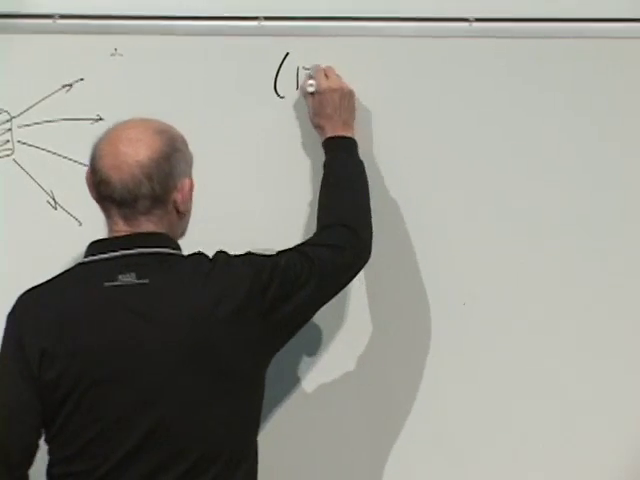
\includegraphics[width=0.66\textwidth]{lecture_06_figure_02.png}
  \caption{La condition de couche de masse dans la convention de métrique utilisée tout au long du cours.}
  \lectureframe{00:05:56}
  \label{fig:l06-mass-shell}
\end{figure}

Considérons deux particules incidentes d’impulsions \(k_1,k_2\) et deux particules émergentes d’impulsions physiques \(q_3,q_4\). La conservation de l’énergie et de l’impulsion s’écrit sous la forme d’une équation unique de quadrivecteurs,
\begin{equation}
  k_1+k_2=q_3+q_4.
  \label{eq:l06-physical-conservation}
\end{equation}
Il est commode d’attribuer une impulsion entrante à chaque ligne externe :
\begin{equation}
  k_3\equiv-q_3,
  \qquad
  k_4\equiv-q_4.
\end{equation}
On a alors
\begin{equation}
  k_1+k_2+k_3+k_4=0,
  \label{eq:l06-all-incoming}
\end{equation}
et chaque ligne vérifie \(k_i^2=-m_i^2\). Les particules émergentes n’ont une énergie négative que dans cette convention de comptabilité ; leurs énergies physiques restent positives.

\begin{figure}[H]
  \centering
  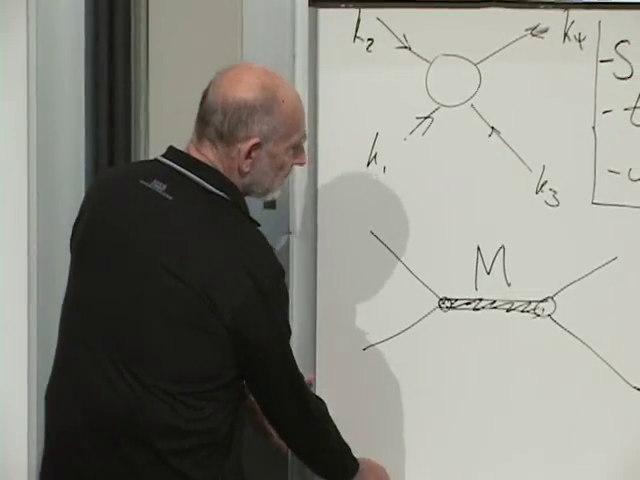
\includegraphics[width=0.68\textwidth]{lecture_06_figure_03.png}
  \caption{On inverse les impulsions physiques des particules émergentes afin de traiter symétriquement comme entrantes les quatre impulsions externes.}
  \lectureframe{00:09:10}
  \label{fig:l06-all-incoming-board}
\end{figure}

Au premier abord, l’amplitude semble être une fonction de seize composantes, \(\mathcal A(k_1,k_2,k_3,k_4)\). La plupart sont redondantes. Passons dans le référentiel du centre de masse, orientons les impulsions incidentes selon un axe choisi et supposons, pour simplifier, que les quatre particules ont la même masse. L’état incident est alors déterminé par un seul nombre : l’énergie du centre de masse. Les impulsions spatiales des particules émergentes doivent être opposées, de même norme, et leur norme doit être égale à celle des impulsions incidentes. Seul leur angle de déflexion \(\theta\) reste à préciser. Le processus dépend donc de deux variables cinématiques indépendantes : \begin{equation}
  E_{\mathrm{cm}},
  \qquad
  \theta.
  \label{eq:l06-two-data}
\end{equation}

\section{Variables de Mandelstam}

Les deux quantités physiques de \eqref{eq:l06-two-data} doivent pouvoir s’exprimer sans choisir de référentiel. Avec la convention où toutes les impulsions sont entrantes, définissons
\begin{equation}
  \begin{aligned}
    -s&=(k_1+k_2)^2,\\
    -t&=(k_1+k_3)^2,\\
    -u&=(k_1+k_4)^2.
  \end{aligned}
  \label{eq:l06-mandelstam}
\end{equation}
Dans le référentiel du centre de masse, les parties spatiales de \(k_1+k_2\) s’annulent ; on a donc
\begin{equation}
  s=E_{\mathrm{cm}}^2.
  \label{eq:l06-s-energy}
\end{equation}

Pour une impulsion physique sortante \(q_3=-k_3\),
\begin{equation}
  k_1+k_3=k_1-q_3
\end{equation}
est l’impulsion transférée de la ligne 1 à la ligne 3. Pour des masses externes égales et une norme \(p\) de l’impulsion spatiale incidente,
\begin{equation}
  -t=2p^2(1-\cos\theta),
  \qquad
  -u=2p^2(1+\cos\theta).
  \label{eq:l06-tu-angle}
\end{equation}
Ainsi, \(t\) et \(u\) portent l’information angulaire mesurée par les détecteurs.

\begin{figure}[H]
  \centering
  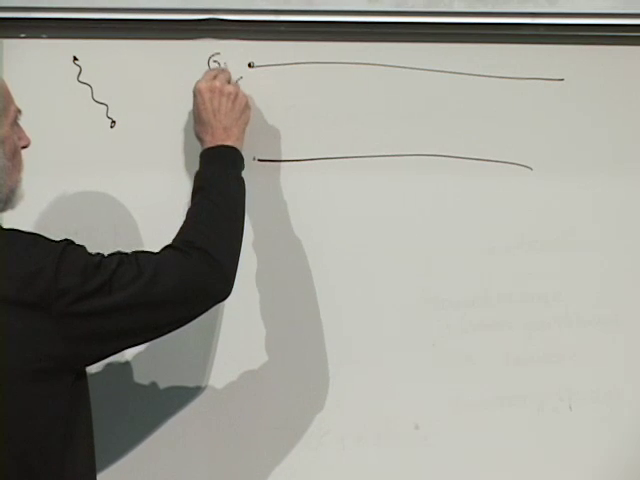
\includegraphics[width=0.74\textwidth]{lecture_06_figure_04.png}
  \caption{Les définitions symétriques de \(s,t,u\) dans la convention où toutes les impulsions sont entrantes.}
  \lectureframe{00:26:20}
  \label{fig:l06-stu-board}
\end{figure}

Trois symboles ne signifient pas qu’il y ait trois données indépendantes. En élevant \eqref{eq:l06-all-incoming} au carré et en utilisant \(k_i^2=-m^2\), on obtient
\begin{equation}
  s+t+u=4m^2
  \label{eq:l06-stu-constraint}
\end{equation}
pour des masses égales. Dès que \(s\) et \(t\) sont connus, \(u\) est fixé.

\begin{classroomqa}
\audiencequestion{Le vide peut-il ralentir une particule en mouvement libre, un peu comme le ferait un frottement ? \lecturetimestamp{00:27:17}}
\lecturerresponse{Pas dans un vide invariant par translation. Il n’y a nulle part où transférer l’impulsion manquante ; la conservation de l’impulsion interdit donc un tel frottement. On peut imaginer un milieu ou un autre vide qui sélectionne un référentiel de repos privilégié, mais ce n’est pas le vide considéré ici.}
\end{classroomqa}

\begin{classroomqa}
\audiencequestion{Pourquoi les deux particules émergentes doivent-elles avoir la même énergie ? \lecturetimestamp{00:27:54}}
\lecturerresponse{Dans le référentiel du centre de masse, leurs impulsions spatiales doivent être opposées et de même norme. Pour le processus à masses égales considéré ici, l’égalité des normes des impulsions entraîne l’égalité des énergies par \(E^2=p^2+m^2\). Si les masses des particules émergentes étaient différentes, cette dernière conclusion devrait être modifiée.}
\end{classroomqa}

\section{Voies directe et croisée}

Dans un diagramme simple de particules ponctuelles, les particules 1 et 2 forment une particule intermédiaire de masse \(M\), qui se désintègre ensuite en 3 et 4. À des facteurs de numérateur et à la prescription de pôles près, la dépendance caractéristique est
\begin{equation}
  \mathcal A_s\sim\frac{g^2}{s-M^2}.
  \label{eq:l06-s-channel}
\end{equation}
C’est le processus de la voie directe, ou voie \(s\). En faisant pivoter la connectivité, on obtient un échange entre les deux lignes externes,
\begin{equation}
  \mathcal A_t\sim\frac{g^2}{t-M^2},
  \label{eq:l06-t-channel}
\end{equation}
qui correspond au processus de la voie croisée, ou voie \(t\). Une troisième connectivité donne
\begin{equation}
  \mathcal A_u\sim\frac{g^2}{u-M^2}.
  \label{eq:l06-u-channel}
\end{equation}

\begin{figure}[H]
  \centering
  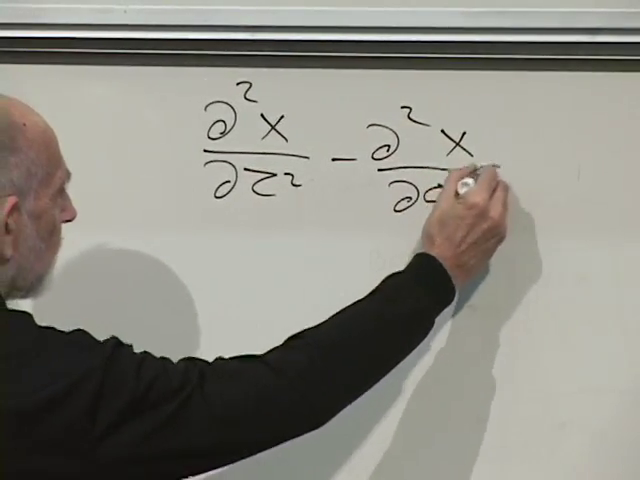
\includegraphics[width=0.72\textwidth]{lecture_06_figure_05.png}
  \caption{Production directe par un état intermédiaire et le pôle correspondant \(g^2/(s-M^2)\) ; la connectivité croisée est représentée sur le même tableau.}
  \lectureframe{00:30:50}
  \label{fig:l06-channel-board}
\end{figure}

La distinction est physique. À ce niveau très rudimentaire, où l’on ne considère que des scalaires, \eqref{eq:l06-s-channel} dépend de l’énergie de collision, mais pas de l’angle. Avant de se désintégrer, l’état composé a perdu la mémoire de la direction incidente ; sa désintégration est donc isotrope. L’amplitude d’échange dépend du transfert d’impulsion et, par conséquent, de l’angle ; une particule échangée légère favorise fortement les faibles déflexions. Le spin ajouterait d’autres dépendances angulaires, mais la structure des pôles est déjà visible.

\begin{classroomqa}
\audiencequestion{La voie \(u\) manquante donne-t-elle un troisième terme ? \lecturetimestamp{00:34:47}}
\lecturerresponse{Oui, dès lors que l’identité des particules et les couplages permettent cette connectivité. On ajoute alors un terme qui présente un pôle en \(u=M^2\). Il ne s’agit pas d’une nouvelle variable cinématique indépendante, puisque \(s+t+u=4m^2\), mais d’un diagramme de canal distinct.}
\end{classroomqa}

\section{Une fonction, deux descriptions de canal}

Un pôle unique décrit mal la diffusion des mésons. Deux mésons peuvent former de nombreuses résonances, avec toute une série de masses et de moments angulaires. Dans les 1960, la première réaction a consisté à ajouter des pôles de la voie \(s\), puis de la voie \(t\), ainsi que les pôles autorisés de la voie \(u\). On a ensuite découvert une fonction bien plus économique. Dans les unités du cours, où la trajectoire de Regge linéaire et son intercept ont été absorbés dans \(s\) et \(t\), elle s’écrit
\begin{equation}
  \mathcal A_{\mathrm V}(s,t)
  \propto
  \frac{\Gamma(-s)\Gamma(-t)}{\Gamma(-s-t)}.
  \label{eq:l06-veneziano}
\end{equation}
La fonction gamma prolonge la factorielle :
\begin{equation}
  \Gamma(n)=(n-1)!
\end{equation}
pour les entiers positifs.

\begin{figure}[H]
  \centering
  \includegraphics[width=0.68\textwidth]{lecture_06_figure_06.png}
  \caption{L’amplitude de Veneziano écrite sous la forme d’un rapport symétrique de fonctions gamma.}
  \lectureframe{00:42:25}
  \label{fig:l06-veneziano-board}
\end{figure}

Les pôles de \(\Gamma(-s)\) reproduisent une série infinie de résonances dans la voie directe. Pourtant, la même expression est symétrique sous \(s\leftrightarrow
t\) ; ses pôles \(\Gamma(-t)\) donnent donc un développement dans la voie croisée. Il ne s’agit pas de deux contributions ajoutées séparément. Une seule fonction analytique admet l’une ou l’autre description. C’est l’ancienne idée de la dualité entre les résonances de la voie directe et les échanges de la voie croisée.

\begin{classroomqa}
\audiencequestion{Comment une amplitude unique peut-elle contenir les deux sommes de canaux sans les additionner ? \lecturetimestamp{00:43:32}}
\lecturerresponse{C’est précisément là que réside la surprise. Le développement de la fonction au voisinage de ses pôles dans la voie \(s\) l’organise en résonances directes ; son développement au voisinage de ses pôles dans la voie \(t\) organise cette même fonction en échanges. Il faut un modèle microscopique pour expliquer pourquoi ces deux lectures coïncident : ce modèle est une corde en interaction.}
\end{classroomqa}

\section{Une bande balayée par une corde ouverte}

Paramétrons une corde ouverte par
\begin{equation}
  0\leq\sigma\leq\pi.
\end{equation}
Le paramètre \(\sigma\) ne désigne pas une position dans l’espace-temps. L’application \(X^\mu(\sigma,\tau)\) indique où se trouve dans l’espace-temps le point ainsi repéré, tandis que \(\tau\) mesure l’évolution. Une particule ponctuelle balaie une ligne d’univers ; la corde en mouvement balaie une feuille d’univers bidimensionnelle. Dans la théorie libre, chaque coordonnée de l’application vérifie
\begin{equation}
  \frac{\partial^2X^\mu}{\partial\tau^2}
  -
  \frac{\partial^2X^\mu}{\partial\sigma^2}
  =0.
  \label{eq:l06-wave-equation}
\end{equation}

\begin{figure}[H]
  \centering
  \includegraphics[width=0.70\textwidth]{lecture_06_figure_07.png}
  \caption{L’équation d’onde qui régit chacune des coordonnées de la corde libre sur la bande de la feuille d’univers.}
  \lectureframe{00:49:10}
  \label{fig:l06-wave-equation-board}
\end{figure}

Pour construire la diffusion, il est utile de ne pas prendre trop tôt la limite continue. Remplaçons chaque corde par \(n\) points matériels reliés par des ressorts. La feuille d’univers devient un ensemble dense de lignes d’univers proches les unes des autres, et ses modes normaux sont de simples oscillateurs harmoniques. Deux chaînes incidentes peuvent se toucher par leurs extrémités. À cet instant, un nouveau ressort les relie ; elles évoluent pendant une durée \(\tau\) comme une chaîne plus longue, puis un ressort se rompt et deux chaînes émergentes se forment à nouveau.

\begin{figure}[H]
  \centering
  \includegraphics[width=0.72\textwidth]{lecture_06_figure_08.png}
  \medskip

  \begin{tikzpicture}[x=0.85cm,y=0.70cm]
    \draw[thick] (0,2.2) -- (2.1,2.2) -- (3.1,1.5);
    \draw[thick] (0,0.8) -- (2.1,0.8) -- (3.1,1.5);
    \draw[thick] (3.1,1.5) -- (5.5,1.5);
    \draw[thick] (5.5,1.5) -- (6.5,2.2) -- (8.6,2.2);
    \draw[thick] (5.5,1.5) -- (6.5,0.8) -- (8.6,0.8);
    \draw[<->] (3.1,0.35) -- node[below] {\(\tau\)} (5.5,0.35);
    \node[left] at (0,2.2) {1};
    \node[left] at (0,0.8) {2};
    \node[right] at (8.6,2.2) {3};
    \node[right] at (8.6,0.8) {4};
  \end{tikzpicture}
  \caption{Deux cordes ouvertes discrétisées se touchent, forment une seule corde intermédiaire pendant une durée \(\tau\), puis se séparent. Le cadre source conserve la construction en ressorts et en lignes d’univers ; le schéma met en évidence leurs connexions.}
  \lectureframe{00:51:25}
  \label{fig:l06-string-joining}
\end{figure}

Les deux cordes ne sont dessinées côte à côte que dans l’espace des paramètres. Leurs positions dans l’espace-temps n’ont pas besoin d’être voisines tant que les coordonnées de leurs extrémités ne coïncident pas effectivement. La liberté de reparamétrisation permet de placer les événements de jonction et de séparation à des positions commodes dans le diagramme ; cette liberté géométrique deviendra la symétrie conforme dans le cours suivant.

\section{Le calcul des oscillateurs, étape par étape}

Désignons les coordonnées de la première chaîne par \(x_1,\ldots,x_n\) et celles de la seconde par \(x_{n+1},\ldots,x_{2n}\). Leurs coordonnées de centre de masse sont
\begin{equation}
  X_{\mathrm{cm}}^{(1)}
  =\frac1n\sum_{a=1}^{n}x_a,
  \qquad
  X_{\mathrm{cm}}^{(2)}
  =\frac1n\sum_{a=n+1}^{2n}x_a.
  \label{eq:l06-chain-centers}
\end{equation}
Une chaîne d’impulsion déterminée \(k_1\) possède une onde plane de centre de masse multipliée par l’état fondamental de ses oscillateurs internes :
\begin{align}
  \Psi_1
  &=
  e^{ik_1\cdot X_{\mathrm{cm}}^{(1)}}
  \psi_0(x_1,\ldots,x_n),
  \\
  \Psi_2
  &=
  e^{ik_2\cdot X_{\mathrm{cm}}^{(2)}}
  \psi_0(x_{n+1},\ldots,x_{2n}).
  \label{eq:l06-two-wavefunctions}
\end{align}
Les facteurs \(\psi_0\) dépendent des coordonnées relatives et non de la translation commune de toute la chaîne. Comme les cordes incidentes constituent initialement des systèmes quantiques distincts,
\begin{equation}
  \Psi_{\mathrm{in}}=\Psi_1\Psi_2.
  \label{eq:l06-product-state}
\end{equation}

\begin{figure}[H]
  \centering
  \includegraphics[width=0.76\textwidth]{lecture_06_figure_09.png}
  \caption{Les deux ondes planes d’impulsion et leurs facteurs d’état fondamental des oscillateurs internes, représentés dans des couleurs distinctes.}
  \lectureframe{00:58:05}
  \label{fig:l06-wavefunctions-board}
\end{figure}

La jonction sélectionne la partie de cette fonction d’onde pour laquelle les coordonnées des deux extrémités coïncident :
\begin{equation}
  x_n=x_{n+1}.
  \label{eq:l06-endpoint-contact}
\end{equation}
À cet instant, les autres coordonnées restent inchangées. L’état sélectionné évolue alors sous l’action de l’hamiltonien \(H_{\mathrm{joined}}\) de la chaîne unique plus longue :
\begin{equation}
  \Psi(\tau)
  =
  e^{-iH_{\mathrm{joined}}\tau}\Psi(0).
  \label{eq:l06-time-evolution}
\end{equation}
Enfin, on calcule son recouvrement avec un produit d’états de cordes émergentes, d’impulsions \(q_3,q_4\).

\begin{figure}[H]
  \centering
  \includegraphics[width=0.76\textwidth]{lecture_06_figure_10.png}
  \caption{La fonction d’onde des deux chaînes juste avant d’imposer la coïncidence de leurs extrémités.}
  \lectureframe{00:58:55}
  \label{fig:l06-endpoint-board}
\end{figure}

Le calcul est long, mais il n’a rien de mystérieux. Chaque coordonnée interne peut être décomposée en modes oscillatoires ; le recouvrement à la jonction, l’évolution temporelle et la projection finale se ramènent donc à de l’algèbre gaussienne des oscillateurs. La durée \(\tau\) pendant laquelle la corde reste jointe est la seule quantité qui ne soit pas fixée.

\begin{classroomqa}
\audiencequestion{Les fonctions d’onde noire et rouge s’additionnent-elles ou se multiplient-elles ? \lecturetimestamp{01:02:26}}
\lecturerresponse{Elles se multiplient. Dans la représentation en coordonnées, l’état produit tensoriel de deux systèmes indépendants est représenté par le produit de leurs fonctions d’onde. Une somme décrirait une superposition de possibilités, et non la présence simultanée des deux cordes incidentes.}
\end{classroomqa}

\begin{classroomqa}
\audiencequestion{Pourquoi intégrer sur le temps intermédiaire \(\tau\) ? \lecturetimestamp{01:04:04}}
\lecturerresponse{On n’attribue pas de durée fixe à la corde jointe. La règle de Feynman consiste à sommer les amplitudes sur toutes les histoires possibles. Dans cette description, le paramètre continu restant pour caractériser l’histoire est la durée entre la jonction et la séparation ; la somme devient donc une intégrale sur \(0\leq\tau<\infty\).}
\end{classroomqa}

\section{Du temps de propagation à la fonction bêta}

Après le calcul des recouvrements des oscillateurs, le résultat peut s’écrire sous la forme
\begin{equation}
  \mathcal A(s,t)
  \propto
  \int_0^\infty d\tau\,
  e^{\tau(s+1)}
  \bigl(1-e^{-\tau}\bigr)^{-t-1}
  e^{-\tau}.
  \label{eq:l06-tau-integral}
\end{equation}
On laisse apparaître le facteur final \(e^{-\tau}\), car il fournit le jacobien nécessaire à l’étape suivante. De façon équivalente, les exponentielles de début et de fin se regroupent en \(e^{s\tau}\).

\begin{figure}[H]
  \centering
  \includegraphics[width=0.76\textwidth]{lecture_06_figure_11.png}
  \caption{L’intégrande en fonction du temps de propagation après le calcul des oscillateurs ; le facteur distinct \(e^{-\tau}\) fournit le jacobien du changement de variable.}
  \lectureframe{01:06:45}
  \label{fig:l06-tau-integral-board}
\end{figure}

Posons maintenant
\begin{equation}
  z=e^{-\tau},
  \qquad
  dz=-e^{-\tau}\,d\tau.
  \label{eq:l06-z-substitution}
\end{equation}
Quand \(\tau\) varie de \(0\) à \(\infty\), \(z\) varie de \(1\) à \(0\). Le signe moins inverse les bornes, d’où
\begin{equation}
  \mathcal A(s,t)
  \propto
  \int_0^1
  z^{-s-1}(1-z)^{-t-1}\,dz.
  \label{eq:l06-beta-integral}
\end{equation}

\begin{figure}[H]
  \centering
  \includegraphics[width=0.74\textwidth]{lecture_06_figure_12.png}
  \caption{Le changement de variable \(z=e^{-\tau}\) fait apparaître l’intégrale bêta d’Euler.}
  \lectureframe{01:08:49}
  \label{fig:l06-beta-integral-board}
\end{figure}

Cette intégrale est définie directement lorsque ses bornes convergent, et ailleurs par prolongement analytique. C’est la fonction bêta d’Euler :
\begin{equation}
  B(-s,-t)
  =
  \frac{\Gamma(-s)\Gamma(-t)}{\Gamma(-s-t)}.
  \label{eq:l06-beta-gamma}
\end{equation}

\begin{figure}[H]
  \centering
  \includegraphics[width=0.72\textwidth]{lecture_06_figure_13.png}
  \caption{Le tableau identifie l’intégrale transformée à \(B(-s,-t)\) et commence à rétablir son expression en fonctions gamma.}
  \lectureframe{01:12:24}
  \label{fig:l06-beta-gamma-board}
\end{figure}

La symétrie entre les voies est maintenant élémentaire. Sous \(z\mapsto1-z\),
\begin{equation}
  \int_0^1 z^{-s-1}(1-z)^{-t-1}\,dz
  =
  \int_0^1 z^{-t-1}(1-z)^{-s-1}\,dz.
\end{equation}
On a donc \(\mathcal A(s,t)=\mathcal A(t,s)\). Un processus construit à partir de deux cordes qui se rejoignent puis se séparent contient automatiquement aussi la description croisée.
\editorialnote{Dans les arguments de la fonction bêta, le cours omet la pente de Regge et l’intercept. Dans la notation standard, on remplace \(s,t\) par les trajectoires linéaires correspondantes \(\alpha(s),\alpha(t)\). La dualité et l’argument fondé sur le changement de variable restent inchangés.}

\begin{classroomqa}
\audiencequestion{Le rapport de fonctions gamma ressemble aux expressions factorielles rencontrées en combinatoire. Existe-t-il une interprétation directe en termes de dénombrement physique ? \lecturetimestamp{01:13:22}}
\lecturerresponse{Pour des arguments entiers, la fonction bêta est liée à un rapport tel que \(n!\,m!/(n+m)!\), mais rien n’affirme ici l’existence d’un mécanisme combinatoire. La même fonction spéciale apparaît dans l’intégrale sur la feuille d’univers ; cette ressemblance n’est pas à l’origine de l’amplitude.}
\end{classroomqa}

La raison, encore cachée, pour laquelle on peut lire une même feuille d’univers dans les deux voies est la symétrie conforme. Elle permet d’étirer la feuille comme de la pâte sans modifier l’amplitude, transformant une longue région de propagation dans la voie directe en une représentation par échange dans la voie croisée. Cette explication géométrique est reportée au cours suivant.

\section{Ce que l’étude de la diffusion a établi}
\enlargethispage{3\baselineskip}
\begingroup
\setlength{\medskipamount}{3pt plus 1pt minus 1pt}

La représentation discrète de la jonction a suscité une dernière série de questions.

\begin{classroomqa}
\audiencequestion{Si deux chaînes de \(n\) constituants se rejoignent par leurs extrémités, le résultat contient-il \(2n-1\) constituants, et cela pourrait-il modifier la parité fermionique ? \lecturetimestamp{01:16:16}}
\lecturerresponse{Dans la représentation hadronique des extrémités, on peut considérer la paire d’extrémités qui se touchent comme une paire particule-antiparticule qui s’annihile ; le nombre diminue donc de deux, et non d’une unité. Dans la limite continue, la différence finie entre \(2n\) et \(2n-2\) est sans importance, mais la conservation de la parité fermionique, elle, ne l’est pas. Les constituants du réseau ne sont qu’un régulateur de la corde continue, et non des grains fondamentaux au sens littéral.}
\end{classroomqa}

\begin{classroomqa}
\audiencequestion{La suite du cours abordera-t-elle les mathématiques complètes des supercordes ? \lecturetimestamp{01:18:05}}
\lecturerresponse{Seules certaines conséquences seront utilisées. La suite immédiate passe par la symétrie de la feuille d’univers et la compactification, puis par un autre point de départ, élaboré au milieu des années 1990s : la théorie M. Son objectif est de retrouver la même physique à partir d’un point de vue qui rend transparentes plusieurs caractéristiques autrement complexes.}
\end{classroomqa}

\begin{classroomqa}
\audiencequestion{Cette règle de jonction n’était-elle qu’un indice tiré des collisions de mésons ? \lecturetimestamp{01:20:02}}
\lecturerresponse{La diffusion des mésons a fourni l’indice historique, mais la règle s’applique de façon générale aux cordes ouvertes. La même topologie décrit les collisions de photons de corde ouverte et d’autres états de corde ouverte. Deux cordes fermées se rejoignent et se séparent selon une construction analogue, avec une corde fermée dans la région intermédiaire.}
\end{classroomqa}

\begin{classroomqa}
\audiencequestion{Le calcul ne s’applique-t-il qu’aux états de corde fermioniques ? \lecturetimestamp{01:20:56}}
\lecturerresponse{Non. Le calcul original de Veneziano concerne la corde ouverte bosonique. Les supercordes exigent des degrés de liberté fermioniques supplémentaires et modifient certains détails de l’intégrande, mais la logique de jonction, de propagation, de projection et de dualité sur la feuille d’univers reste très analogue.}
\end{classroomqa}

La présence d’un état de spin un ou deux dans le spectre des oscillateurs était suggestive, mais ne constituait pas une preuve décisive. Les amplitudes de diffusion correspondantes ont fourni un test plus probant. Les amplitudes des photons satisfont les identités associées à la conservation de la charge et à l’invariance de jauge ; celles des gravitons satisfont les contraintes correspondantes d’un champ sans masse de spin deux. Les états de la corde ont satisfait ces tests dans leurs interactions entre eux, ainsi qu’avec des états massifs et sans masse. C’est pourquoi les appellations de photon et de graviton sont devenues des identifications physiques plutôt que de simples hypothèses fondées sur le dénombrement des polarisations.
\editorialnote{Dans le langage moderne, ces tests s’expriment par le découplage des polarisations non physiques, les identités de Ward de jauge et le couplage universel à basse énergie de l’état sans masse de spin deux.}

\begin{classroomqa}
\audiencequestion{D’où vient la charge électrique elle-même dans la description par les cordes ? \lecturetimestamp{01:24:03}}
\lecturerresponse{Le cours s’achève sans répondre à cette question. La réponse exige de connaître la structure interne et la structure des extrémités de la théorie des cordes, qui n’ont pas encore été introduites ; elle relève donc de la suite du cours plutôt que de cette dérivation de la diffusion.}
\end{classroomqa}
\endgroup

\chapter{Feuilles d’univers, rotation de Wick et dualité des canaux}

\lectureoverview{Une particule décrit une ligne d’univers ; une corde engendre une feuille d’univers. Quantifier l’un ou l’autre objet exige une somme sur les histoires, mais la somme lorentzienne est oscillante et difficile à définir. En faisant du temps de la feuille d’univers une coordonnée imaginaire, on obtient une théorie euclidienne régie par l’équation de Laplace. Sa symétrie conforme permet alors de transformer la surface fendue d’une interaction entre quatre cordes en un disque portant quatre insertions sur son bord ; la symétrie entre les canaux direct et croisé y devient manifeste.}

\section{De la ligne d’univers à la somme sur les histoires}

Considérons d’abord une particule libre. En mécanique non relativiste, sa position est une fonction \(\mathbf x(t)\) et, en prenant la masse égale à un, son action s’écrit
\begin{equation}
  S_{\mathrm{NR}}[\mathbf x]
  =\frac12\int_{t_1}^{t_2}\dot{\mathbf x}^{\,2}\,dt.
  \label{eq:l07-nr-action}
\end{equation}
Pour une description relativiste, il est plus naturel de réunir le temps et l’espace dans un même vecteur, \(X^\mu(\tau)\), paramétré le long de la trajectoire par \(\tau\). L’expression quadratique correspondante est
\begin{equation}
  S_{\mathrm{rel}}[X]
  =\frac12\int_{\tau_1}^{\tau_2}
  \frac{dX^\mu}{d\tau}\frac{dX_\mu}{d\tau}\,d\tau.
  \label{eq:l07-rel-action}
\end{equation}
Les indices hauts et bas encodent la différence de signe lorentzienne entre le temps et l’espace.
\editorialnote{L’action relativiste quadratique est ici écrite pour une paramétrisation fixée de la ligne d’univers. L’autre possibilité, manifestement invariante par reparamétrisation, est proportionnelle à la longueur propre ; elle sera évoquée plus loin dans le cours.}

\begin{figure}[H]
  \centering
  \includegraphics[width=0.72\textwidth]{lecture_07_figure_01.png}
  \caption{L’action non relativiste et son analogue relativiste quadratique, écrits côte à côte au tableau.}
  \lectureframe{00:03:35}
  \label{fig:l07-particle-actions}
\end{figure}

Classiquement, on fixe les extrémités et on fait varier le chemin. Une particule libre suit alors une ligne d’univers droite, à vitesse constante. La mécanique quantique pose une autre question. Elle ne sélectionne pas une trajectoire unique entre les extrémités : elle demande quelle est l’amplitude pour partir d’un point et être détecté à l’autre. Chaque chemin intermédiaire contribue avec une phase,
\begin{equation}
  K(2,1)=\int_{X(1)}^{X(2)}\!\mathcal D X\,
  e^{iS[X]}.
  \label{eq:l07-feynman-integral}
\end{equation}
L’intégrale fonctionnelle est une intégrale sur un espace de chemins de dimension infinie, et non l’intégrale ordinaire qui figure déjà dans l’action.

\begin{figure}[H]
  \centering
  \includegraphics[width=0.72\textwidth]{lecture_07_figure_02.png}
  \caption{Un chemin représentatif et la phase qui lui est associée avant la somme sur toutes les trajectoires.}
  \lectureframe{00:06:21}
  \label{fig:l07-path-integral-board}
\end{figure}

En langage relativiste, cette amplitude entre deux points est un propagateur. Lors d’une interaction, plusieurs segments de ligne d’univers se rejoignent. On additionne leurs actions, on intègre sur les points de rencontre et on somme les diagrammes comportant les particules externes requises. Ainsi, le développement familier en diagrammes de Feynman est déjà implicitement contenu dans l’instruction de sommer sur les histoires.

Le symbole \(S\) désignera ici une action. Il n’a de lien ni avec l’entropie ni avec la variable de Mandelstam \(s\) utilisée vers la fin du cours. Cette notation commune relève de la tradition plutôt que de la clarté.

\section{Faire pivoter le temps}

\eqref{eq:l07-feynman-integral} pose immédiatement un problème. Chaque facteur \(e^{iS}\) a un module égal à un. Une trajectoire qui oscille de façon désordonnée et la ligne droite classique entrent donc dans la somme avec le même poids en valeur absolue ; seules leurs phases diffèrent. L’interférence destructive permet de retrouver le comportement classique, mais ne transforme pas l’intégrale formelle en un objet ordinaire convergent.

Introduisons un nouveau paramètre \(s\) défini par
\begin{equation}
  \tau=\alpha s,
  \qquad
  d\tau=\alpha\,ds,
  \qquad
  \frac{dX}{d\tau}=\frac{1}{\alpha}\frac{dX}{ds}.
\end{equation}
L’action quadratique se transforme alors comme suit :
\begin{equation}
  \frac12\int d\tau
  \left(\frac{dX}{d\tau}\right)^2
  =
  \frac{1}{2\alpha}\int ds
  \left(\frac{dX}{ds}\right)^2.
  \label{eq:l07-rescaled-action}
\end{equation}
Le choix du contour correspondant à \(\alpha=-i\) transforme le poids oscillant en
\begin{equation}
  e^{iS}
  \longrightarrow
  \exp\!\left[-\frac12\int ds
  \left(\frac{dX}{ds}\right)^2\right]
  =e^{-S_E}.
  \label{eq:l07-euclidean-particle}
\end{equation}

\begin{figure}[H]
  \centering
  \includegraphics[width=0.66\textwidth]{lecture_07_figure_03.png}
  \caption{Le poids euclidien de la particule après la substitution du temps imaginaire ; l’exposant est réel et non positif.}
  \lectureframe{00:16:20}
  \label{fig:l07-particle-wick}
\end{figure}

Un chemin qui s’éloigne beaucoup avant de revenir, ou qui oscille rapidement sans beaucoup se déplacer, a une grande action positive \(S_E\) et est donc exponentiellement supprimé. On obtient une intégrale de type Wiener, pour laquelle il existe une théorie de la convergence rigoureuse. Les extrémités héritées du \(\tau\) réel se trouvent sur un contour \(s\) imaginaire. En pratique, on évalue l’objet euclidien dans son domaine de convergence, puis on prolonge analytiquement le résultat aux variables lorentziennes physiques. C’est la rotation de Wick : pour le calcul, on a fait pivoter le temps, on ne l’a pas supprimé.

\section{Des lignes d’univers aux feuilles d’univers}

Une particule ponctuelle a une ligne d’univers. Une corde ouverte engendre un ruban, et une corde fermée, un tube. Les coordonnées \((\sigma,\tau)\) repèrent les points de cette feuille d’univers bidimensionnelle, tandis que
\begin{equation}
  X^\mu=X^\mu(\sigma,\tau)
  \label{eq:l07-embedding}
\end{equation}
donne la position dans l’espace-temps du point repéré. La connaissance de toutes les fonctions \(X^\mu\) spécifie l’histoire complète de la corde.

L’action quadratique lorentzienne sur la feuille d’univers a la même structure cinétique moins potentiel que celle d’une corde vibrante ordinaire :
\begin{equation}
  S_{\mathrm{ws}}[X]
  =\frac{T_s}{2}\int d\tau\,d\sigma\,
  \left[
    \partial_\tau X^\mu\partial_\tau X_\mu
    -
    \partial_\sigma X^\mu\partial_\sigma X_\mu
  \right].
  \label{eq:l07-lorentzian-worldsheet}
\end{equation}
La tension totale \(T_s\) fixe l’échelle ; le cours la laisse de côté pour se concentrer sur la structure des dérivées.

\begin{figure}[H]
  \centering
  \includegraphics[width=0.72\textwidth]{lecture_07_figure_04.png}
  \caption{L’action lorentzienne sur la feuille d’univers pour \(X^\mu(\sigma,\tau)\), avec son signe cinétique moins potentiel.}
  \lectureframe{00:24:26}
  \label{fig:l07-worldsheet-action}
\end{figure}

On obtient l’amplitude de la corde en exponentiant cette action et en sommant sur toutes les surfaces qui relient les configurations initiale et finale prescrites de la corde :
\begin{equation}
  \mathcal A=\int\mathcal D X\,e^{iS_{\mathrm{ws}}[X]}.
  \label{eq:l07-surface-integral}
\end{equation}
La même règle s’applique à deux cordes qui en deviennent deux, à deux qui en deviennent trois, ou à toute autre configuration externe autorisée. Les différentes topologies de feuilles d’univers font également partie de la somme. Ajouter des trous aux surfaces est l’analogue, pour les cordes, de l’ajout de boucles dans le développement en diagrammes pour les particules ponctuelles.

\begin{figure}[H]
  \centering
  \includegraphics[width=0.66\textwidth]{lecture_07_figure_05.png}
  \caption{Une surface reliant plusieurs cordes externes, avec un trou représentant une topologie différente de la feuille d’univers.}
  \lectureframe{00:27:14}
  \label{fig:l07-surface-topology}
\end{figure}

\begin{classroomqa}\audiencequestion{Pour un électron ponctuel, la dérivée par rapport à \(\sigma\) ne s’annule-t-elle pas tout simplement ? \lecturetimestamp{00:27:56}}\lecturerresponse{Une particule ponctuelle n’a pas de coordonnée \(\sigma\) au départ. Les représentations restent néanmoins liées : lorsque les états externes sont légers par rapport à l’échelle de la corde et que les énergies des processus sont faibles, les amplitudes des cordes reproduisent les diagrammes de Feynman ordinaires des particules ponctuelles. Cette limite ne revient pas simplement à annuler une dérivée.}\end{classroomqa}

L’intégrale sur les surfaces présente le même problème de convergence que l’intégrale sur les chemins. Après rotation de Wick du temps sur la feuille d’univers, sa forme euclidienne stable est
\begin{equation}
  \begin{aligned}
    S_{E,\mathrm{ws}}[X]
    &=\frac{T_s}{2}\int d\tau\,d\sigma\,
      \left[
        \partial_\tau X^\mu\partial_\tau X_\mu
        +\partial_\sigma X^\mu\partial_\sigma X_\mu
      \right],\\
    \mathcal A_E&=\int\mathcal D X\,e^{-S_{E,\mathrm{ws}}}.
  \end{aligned}
  \label{eq:l07-euclidean-worldsheet}
\end{equation}
Les deux dérivées interviennent maintenant avec le même signe positif. Une surface qui vibre violemment ou qui est fortement étirée a une grande action euclidienne et est supprimée.

\begin{figure}[H]
  \centering
  \includegraphics[width=0.72\textwidth]{lecture_07_figure_06.png}
  \caption{La densité euclidienne positive sur la feuille d’univers après la rotation de \(\tau\) vers le temps imaginaire.}
  \lectureframe{00:34:29}
  \label{fig:l07-worldsheet-wick}
\end{figure}

Il existe aussi une formulation géométrique directe. On peut associer à une particule relativiste une action proportionnelle à la longueur propre de son chemin, et à une corde, une action proportionnelle à l’aire dans l’espace-temps de sa feuille d’univers. La seconde est l’action de Nambu--Goto. La forme quadratique sur la feuille d’univers utilisée ici est appelée conventionnellement forme de Polyakov ; elle est bien plus facile à manier pour le calcul présent.
\editorialnote{Le cours comporte une remarque humoristique sur les dénominations historiques et mentionne également l’action de Liouville et les conditions aux limites de Dirichlet. Il n’est pas nécessaire de revendiquer une priorité pour cette dérivation : seule est utilisée l’équivalence entre les formulations en termes d’aire et de métrique auxiliaire.}

\section{L’équation du mouvement euclidienne}

Les coordonnées \(\sigma\) et \(\tau\) ne sont que des repères sur la feuille. La question suivante s’impose donc : quels changements de repères laissent la théorie inchangée ? L’équation du mouvement permet de le voir facilement. En faisant varier \eqref{eq:l07-euclidean-worldsheet}, on obtient, composante par composante,
\begin{equation}
  \partial_\tau^2X^\mu+\partial_\sigma^2X^\mu=0.
  \label{eq:l07-laplace}
\end{equation}
Avant la rotation de Wick, le signe relatif est négatif et il s’agit d’une équation d’onde. En signature euclidienne, les deux signes sont positifs : c’est donc l’équation de Laplace en deux dimensions.

\begin{classroomqa}\audiencequestion{Est-ce l’équation d’un tambour vibrant ?
\lecturetimestamp{00:41:50}}\lecturerresponse{Elle lui est étroitement apparentée, mais un tambour vibrant comporte aussi une coordonnée de temps réel et obéit donc à une équation d’onde. L’équation considérée ici est l’équation de Laplace euclidienne. Le potentiel électrostatique dans une région sans charges en est un exemple familier plus direct.}\end{classroomqa}

\begin{classroomqa}\audiencequestion{L’action contient des dérivées premières. Pourquoi son équation contient-elle des dérivées secondes ? \lecturetimestamp{00:42:44}}\lecturerresponse{Faire varier un terme quadratique en une dérivée première, puis intégrer par parties, revient à déplacer une dérivée sur cette dérivée première. C’est l’analogue, en théorie des champs, du fait que \(\dot x^{\,2}\) dans une action produit \(\ddot x\) dans l’équation du mouvement.}\end{classroomqa}

\begin{figure}[H]
  \centering
  \includegraphics[width=0.68\textwidth]{lecture_07_figure_07.png}
  \caption{L’équation de Laplace avec des signes positifs et la première ligne discrète qui sert à interpréter ses dérivées secondes.}
  \lectureframe{00:43:30}
  \label{fig:l07-laplace-board}
\end{figure}

Pour visualiser la géométrie, discrétisons d’abord une coordonnée avec un pas de \(\epsilon\). Une dérivée première est une différence entre points voisins, tandis qu’une dérivée seconde est une différence entre différences voisines :
\begin{equation}
  \frac{d^2X}{ds^2}\bigg|_{2}
  \longrightarrow
  \frac{X(3)-2X(2)+X(1)}{\epsilon^2}.
  \label{eq:l07-second-difference}
\end{equation}

\begin{figure}[H]
  \centering
  \includegraphics[width=0.72\textwidth]{lecture_07_figure_08.png}
  \caption{La ligne numérotée, un petit morceau de réseau et le développement aux différences finies d’une dérivée seconde.}
  \lectureframe{00:45:51}
  \label{fig:l07-finite-difference-board}
\end{figure}

Discrétisons maintenant le plan \((\sigma,\tau)\). Repérons les quatre plus proches voisins d’un point central \(5\) par \(1,2,3,4\). L’équation
\eqref{eq:l07-laplace} devient
\begin{equation}
  X(1)+X(2)+X(3)+X(4)-4X(5)=0,
\end{equation}
ou encore
\begin{equation}
  X(5)=\frac14\bigl[X(1)+X(2)+X(3)+X(4)\bigr].
  \label{eq:l07-mean-value}
\end{equation}

\begin{figure}[H]
  \centering
  \includegraphics[width=0.72\textwidth]{lecture_07_figure_09.png}
  \caption{L’équation bidimensionnelle aux différences finies obtenue : la valeur au centre est égale à la moyenne de ses quatre voisines.}
  \lectureframe{00:48:26}
  \label{fig:l07-mean-value-board}
\end{figure}

Cette propriété de la valeur moyenne vaut pour un carré infinitésimal quelle que soit son orientation. Elle exprime le contenu géométrique local de l’équation de Laplace et établit le lien avec la symétrie conforme.

\section{Coordonnées conformes}

Considérons un changement de \((\sigma,\tau)\) en \((\sigma',\tau')\). Une déformation générale transforme un petit carré en un quadrilatère quelconque. Les transformations qui nous intéressent ici ont ceci de particulier qu’elles transforment chaque carré infinitésimal en un autre carré infinitésimal, éventuellement tourné et redimensionné. De manière équivalente, elles préservent les angles entre les courbes qui se coupent. Ce sont les transformations conformes.

\begin{figure}[H]
  \centering
  \includegraphics[width=0.68\textwidth]{lecture_07_figure_10.png}
  \caption{Un carré local transformé en une autre petite figure, dont on vérifie la préservation des angles par la transformation conforme.}
  \lectureframe{00:53:25}
  \label{fig:l07-conformal-board}
\end{figure}

\begin{classroomqa}\audiencequestion{Si les angles sont préservés, la transformation se réduit-elle essentiellement à une rotation ? \lecturetimestamp{00:53:31}}\lecturerresponse{Cela n’est vrai que localement ; même localement, un changement d’échelle uniforme est également permis. La rotation et le facteur d’échelle locaux peuvent varier d’un point à l’autre : le réseau de coordonnées peut donc se courber, s’agrandir dans une région et se contracter dans une autre, tout en préservant les formes infinitésimales.}\end{classroomqa}

Une application qui préserve les angles ne préserve pas nécessairement les dimensions. Si celles-ci étaient aussi conservées partout, il ne resterait que la classe bien plus restreinte des transformations rigides : les translations et les rotations. Les applications conformes préservent plutôt la forme locale. C’est pourquoi une projection cartographique peut préserver la forme d’une petite île tout en déformant considérablement son aire.

\begin{classroomqa}\audiencequestion{Une application conforme signifie-t-elle que le système de coordonnées est plat ? \lecturetimestamp{00:55:35}}\lecturerresponse{Non. La platitude et la conformalité sont deux propriétés différentes. Une application conforme peut utiliser des lignes de coordonnées courbes ; elle préserve l’angle entre les courbes qui se coupent. Une projection cartographique de type Mercator est un exemple familier de préservation locale des formes accompagnée d’une forte déformation des échelles.}\end{classroomqa}

En deux dimensions, les transformations requises sont engendrées localement par des fonctions analytiques d’une coordonnée complexe
\begin{equation}
  z=\sigma+i\tau.
\end{equation}
Les frontières finies peuvent changer d’apparence de façon spectaculaire. Une région carrée peut être envoyée sur une région aux contours lisses, les coins initiaux devenant des points ordinaires du nouveau bord plutôt que ses points visuellement les plus saillants. Il n’y a pas de contradiction : la conformalité est une propriété locale à l’intérieur de la région, et l’application préserve les angles infinitésimaux partout où elle est régulière.

\begin{classroomqa}\audiencequestion{Cette liberté de choix des coordonnées explique-t-elle pourquoi le diagramme précédent de jonction--séparation pouvait être choisi symétrique ?
\lecturetimestamp{00:56:32}}\lecturerresponse{Oui. La même liberté conforme qui préserve les équations de la feuille d’univers nous permet de remplacer la bande d’interaction peu commode par un domaine plus symétrique. La liberté restante n’élimine pas le paramètre physique de jonction--séparation ; elle le reformule comme la position relative des insertions sur le bord.}\end{classroomqa}

\section{De la feuille fendue au disque}

Revenons à la diffusion de quatre cordes. Deux cordes ouvertes entrent, leurs extrémités se rejoignent, la corde résultante se propage, puis se sépare. Représenté sur une feuille d’univers plane, le processus forme une bande infinie fendue à chaque extrémité. La distance \(\tau_0\) entre les pointes des fentes est la durée de vie de la corde intermédiaire, et l’amplitude s’intègre sur cette durée.

\begin{figure}[H]
  \centering
  \includegraphics[width=0.72\textwidth]{lecture_07_figure_11.png}
  \caption{La bande à deux fentes représentant la jonction de deux cordes ouvertes, leur propagation commune, puis leur séparation.}
  \lectureframe{01:00:20}
  \label{fig:l07-slit-strip}
\end{figure}

Après euclidisation, les champs d’immersion sur cette région satisfont à l’équation de Laplace. L’invariance conforme permet donc de transformer la bande fendue en disque. On peut se représenter la topologie en feuilletant le disque par des cercles concentriques, puis en déformant continûment ces courbes fermées jusqu’à ce qu’elles remplissent la région fendue. Par l’application, les extrémités à l’infini deviennent des points exceptionnels du bord.

\begin{figure}[H]
  \centering
  \includegraphics[width=0.72\textwidth]{lecture_07_figure_12.png}
  \medskip

  \begin{adjustbox}{max width=\linewidth}
  \begin{tikzpicture}[x=0.75cm,y=0.75cm]
    \draw[thick] (-5,1.2) -- (-1.2,1.2) -- (-0.35,0.35);
    \draw[thick] (-5,-1.2) -- (-1.2,-1.2) -- (-0.35,-0.35);
    \draw[thick] (0.35,0.35) -- (1.2,1.2) -- (5,1.2);
    \draw[thick] (0.35,-0.35) -- (1.2,-1.2) -- (5,-1.2);
    \draw[->,thick] (5.6,0) -- (7.0,0);
    \draw[thick] (9.0,0) circle (1.45);
    \foreach \a in {40,140,220,320} \fill (9.0,0) ++(\a:1.45) circle (1.5pt);
    \node[below] at (0,-1.65) {slit strip};
    \node[below] at (9.0,-1.65) {disc};
  \end{tikzpicture}
  \end{adjustbox}
  \caption{Comparaison au tableau des courbes de niveau et schéma clair de l’application conforme de la bande fendue sur un disque. Les quatre extrémités externes deviennent quatre points particuliers du bord.}
  \lectureframe{01:04:46}
  \label{fig:l07-strip-to-disc}
\end{figure}

Les états externes ne disparaissent pas lors de ce changement de coordonnées. Il faut insérer l’impulsion, le type de particule et le niveau d’oscillation aux quatre points exceptionnels. Les objets formels qui portent ces informations sont les opérateurs de vertex. Leur construction détaillée sera présentée plus tard, mais leur rôle est déjà clair : ils transforment une intégrale de chemin sur une feuille d’univers autrement homogène en une expérience de diffusion spécifiée.

Après avoir utilisé les transformations conformes du disque pour placer trois points du bord à des positions de référence commodes, il reste une position relative réelle. On peut la représenter par le birapport des quatre points ordonnés du bord. C’est l’analogue, sur le disque, de l’ancienne durée de vie \(\tau_0\).

\begin{figure}[H]
  \centering
  \includegraphics[width=0.62\textwidth]{lecture_07_figure_13.png}
  \caption{Quatre points d’insertion sur le bord du disque. La liberté conforme élimine tous les degrés de liberté de leur configuration ordonnée, à l’exception d’un module réel.}
  \lectureframe{01:10:55}
  \label{fig:l07-four-points}
\end{figure}

L’intégrale sur la durée de vie n’a donc pas disparu. Elle est devenue une intégrale sur le module restant. Avec la coordonnée conventionnelle \(0<z<1\), l’intégrale à quatre points pour les cordes ouvertes prend la même forme que dans le cours précédent,
\begin{equation}
  \mathcal A(s,t)\propto
  \int_0^1 z^{-s-1}(1-z)^{-t-1}\,dz.
  \label{eq:l07-modulus-integral}
\end{equation}

\section{Deux limites d’une même surface}

À une extrémité de l’espace des modules, les deux points d’insertion associés à la paire entrante se rapprochent. Dans les coordonnées de la bande fendue, cela correspond à un long intervalle entre la jonction et la séparation : une corde intermédiaire du canal direct se propage pendant longtemps. À l’autre extrémité, une autre paire de points voisins se rapproche. On interprète alors naturellement la même surface comme un échange dans le canal croisé. Sur la bande, ces descriptions semblent sans rapport, mais elles correspondent à deux limites voisines du bord de l’intégrale sur le disque.

Revenons à la convention majoritairement positive du cours précédent :
\begin{equation}
  -s=(k_1+k_2)^2,
  \qquad
  -t=(k_1+k_3)^2.
  \label{eq:l07-mandelstam}
\end{equation}
La limite directe organise les pôles en \(s\) ; la limite croisée organise les pôles en \(t\).
\editorialnote{Vers la fin du cours, le tableau utilise une convention de signe abrégée pour les invariants de Mandelstam, tout en identifiant \(s\) à l’énergie au centre de masse au carré, qui est positive. L’équation \eqref{eq:l07-mandelstam} conserve la convention majoritairement positive établie dans le cours 6.}

\begin{figure}[H]
  \centering
  \includegraphics[width=0.62\textwidth]{lecture_07_figure_14.png}
  \caption{Les diagrammes des deux canaux : une longue propagation dans une orientation, et un échange dans l’orientation croisée.}
  \lectureframe{01:19:27}
  \label{fig:l07-channel-diagrams}
\end{figure}

\begin{figure}[H]
  \centering
  \includegraphics[width=0.72\textwidth]{lecture_07_figure_15.png}
  \caption{Le tableau revient aux appariements des impulsions dans les canaux \(s\) et \(t\), en comparant les deux limites du module du disque.}
  \lectureframe{01:19:40}
  \label{fig:l07-st-board}
\end{figure}

Un seul objet analytique fournit donc les deux développements :
\begin{equation}
  \mathcal A(s,t)=\mathcal A(t,s).
\end{equation}
C’est la dualité des canaux. Dans le langage d’origine des résonances, il semblait miraculeux qu’une somme sur les états du canal direct puisse également rendre compte de l’échange dans le canal croisé. Sur la feuille d’univers euclidienne, la symétrie conforme explique pourquoi ces deux descriptions correspondent à une seule et même surface. Historiquement, cette interprétation a suivi de très près la découverte, en 1969, de l’amplitude de Veneziano.

\begin{classroomqa}\audiencequestion{Existe-t-il aussi une représentation en bande fendue correspondant à l’orientation croisée ? \lecturetimestamp{01:20:49}}\lecturerresponse{Oui, mais il faut choisir différemment la direction appelée temps. On peut découper la même surface euclidienne de sorte qu’une autre paire d’extrémités externes se trouve dans le passé lointain et le futur lointain. C’est précisément parce qu’on peut choisir ce découpage autrement qu’une même feuille d’univers admet plusieurs interprétations en termes de canaux.}\end{classroomqa}

\begin{classroomqa}\audiencequestion{La durée pendant laquelle les cordes restent jointes est-elle déterminée par la constante de couplage ? \lecturetimestamp{01:21:39}}\lecturerresponse{Aucune durée de vie fixe n’est sélectionnée. La durée de vie est une variable d’intégration, et chaque valeur contribue. Le couplage règle le poids associé à la jonction et à la séparation---autrement dit, l’intensité de désintégration---et intervient multiplicativement dans l’amplitude ; il ne remplace pas l’intégrale sur le module.}\end{classroomqa}
\chapter{Applications conformes et prescription de diffusion des cordes ouvertes}

\lectureoverview{Les applications conformes apparaissent d’abord comme une symétrie pratique de l’électrostatique bidimensionnelle. La différentiabilité complexe rend cette symétrie calculable : les équations de Cauchy--Riemann impliquent l’équation de Laplace, et une dérivée complexe indépendante de la direction préserve les angles. Grâce à ces outils, on peut représenter la surface d’univers d’une corde sous la forme d’une bande, d’un demi-plan, d’un cylindre ou d’un disque sans modifier la physique. La diffusion des cordes ouvertes se ramène alors à une intégrale de chemin gaussienne sur le disque, avec des insertions de quantité de mouvement sur son bord, suivie d’une intégration sur leurs positions non équivalentes.}

\section{Électrostatique dans un monde bidimensionnel}

Commençons par un problème d’électrostatique strictement bidimensionnel. Les charges et leurs lignes de champ sont confinées à un plan ; il ne s’agit pas simplement de charges ordinaires tridimensionnelles dont le mouvement se ferait dans un plan. La loi de Gauss donne alors
\begin{equation}
  F(r)\propto \frac{1}{r},
  \qquad
  V(r)\propto \log r,
  \label{eq:l08-two-dimensional-coulomb}
\end{equation}
car le flux traverse un cercle dont la circonférence croît comme \(r\).

Écrivons le champ à l’aide d’un potentiel scalaire \(\phi\). Avec la convention de signe utilisée au tableau,
\begin{equation}
  \mathbf E=\nabla\phi,
  \qquad
  \nabla\cdot\mathbf E=\rho,
\end{equation}
et donc
\begin{equation}
  \nabla^2\phi
  =\frac{\partial^2\phi}{\partial x^2}
  +\frac{\partial^2\phi}{\partial y^2}
  =\rho.
  \label{eq:l08-poisson}
\end{equation}
Dans une région sans charge, cela se réduit à l’équation de Laplace,
\begin{equation}
  \nabla^2\phi=0.
  \label{eq:l08-laplace-phi}
\end{equation}
\editorialnote{De nombreux textes d’électrodynamique définissent
\(\mathbf E=-\nabla\Phi\), auquel cas
\(\nabla^2\Phi=-\rho\) après absorption des constantes. Dans ce cours, le signe du potentiel est choisi à l’opposé. L’équation sans source et tous les arguments conformes restent inchangés.}

\begin{figure}[H]
  \centering
  \includegraphics[width=0.72\textwidth]{lecture_08_figure_01.png}
  \caption{Les équations de l’électrostatique mises sous la forme de l’opérateur de Poisson bidimensionnel.}
  \lectureframe{00:03:48}
  \label{fig:l08-electrostatics-board}
\end{figure}

Le signe plus entre les deux dérivées spatiales est essentiel. Il fait de cette équation une équation elliptique, et non une équation d’onde. Les transformations conformes préservent sa forme sans source : une solution sur un domaine peut donc être transportée vers un domaine de forme différente, avec ses conditions aux limites. Cette propriété est utile en électrostatique, en mécanique des fluides bidimensionnelle et en cartographie, avant de l’être en théorie des cordes.

\begin{classroomqa}
\audiencequestion{Si le laplacien s’annule, s’agit-il d’une équation d’onde stationnaire ? \lecturetimestamp{00:05:35}}
\lecturerresponse{Non. Les deux dérivées spatiales ont le même signe, et il n’y a pas de dérivée temporelle. Une équation d’onde exige une dépendance temporelle avec le signe relatif lorentzien. L’électrostatique est précisément statique : rien n’évolue, pas même une onde.}
\end{classroomqa}

\begin{classroomqa}
\audiencequestion{Existe-t-il un rotationnel en deux dimensions ?
\lecturetimestamp{00:06:06}}
\lecturerresponse{Oui, mais il n’a qu’une seule composante indépendante. Pour
\(\mathbf E=(E_x,E_y)\),
\[
  \operatorname{curl}_{2d}\mathbf E
  =\partial_yE_x-\partial_xE_y.
\]
On peut se le représenter comme la composante perpendiculaire au tableau, même si un monde intrinsèquement bidimensionnel n’a pas besoin d’une direction perpendiculaire extérieure. En dimension supérieure, l’objet correspondant est naturellement une 2-forme antisymétrique.}
\end{classroomqa}

\section{Une dérivée sans direction privilégiée}

Introduisons des coordonnées complexes dans les plans de départ et d’arrivée :
\begin{equation}
  z=x+iy,
  \qquad
  w=u+iv,
  \qquad
  w=w(z).
  \label{eq:l08-complex-coordinates}
\end{equation}
Ici, \(x,y,u,v\) sont réels. Localement, la dérivée devrait être
\begin{equation}
  \frac{dw}{dz}
  =\lim_{\Delta z\to0}\frac{\Delta w}{\Delta z}.
  \label{eq:l08-complex-derivative}
\end{equation}
Contrairement à la droite réelle, le plan complexe admet une infinité de directions d’approche. Une application continue et, en général, régulière ne donne pas nécessairement le même rapport dans toutes ces directions.

Comparons deux approches simples. Dans la direction \(x\), \(dy=0\), donc
\begin{equation}
  \left.\frac{dw}{dz}\right|_x
  =\frac{\partial u}{\partial x}
  +i\frac{\partial v}{\partial x}.
\end{equation}
Dans la direction \(y\), \(dx=0\), et
\begin{equation}
  \left.\frac{dw}{dz}\right|_y
  =\frac{1}{i}\frac{\partial u}{\partial y}
  +\frac{\partial v}{\partial y}
  =\frac{\partial v}{\partial y}
  -i\frac{\partial u}{\partial y}.
\end{equation}
L’égalité des parties réelle et imaginaire donne
\begin{equation}
  \boxed{
  \frac{\partial u}{\partial x}
  =\frac{\partial v}{\partial y},
  \qquad
  \frac{\partial u}{\partial y}
  =-\frac{\partial v}{\partial x}}
  \label{eq:l08-cauchy-riemann}
\end{equation}
Ce sont les équations de Cauchy--Riemann. Sous les hypothèses usuelles de différentiabilité, elles suffisent aussi à garantir que la limite
\eqref{eq:l08-complex-derivative} est indépendante de la direction. Une fonction qui possède cette propriété est dite analytique, ou holomorphe, au point considéré.

\begin{figure}[H]
  \centering
  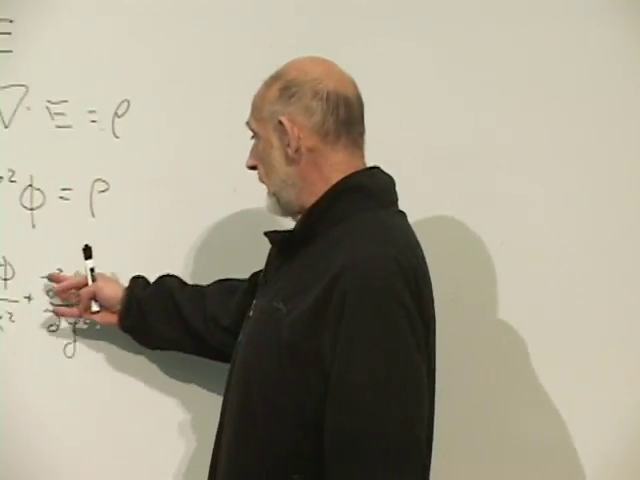
\includegraphics[width=0.70\textwidth]{lecture_08_figure_02.png}
  \caption{Le système complet de Cauchy--Riemann, avec le signe moins relatif.}
  \lectureframe{00:19:48}
  \label{fig:l08-cr-board}
\end{figure}

Le cours distingue brièvement des termes apparentés. Une fonction holomorphe sur tout le plan complexe fini est dite entière. Une fonction méromorphe peut avoir des pôles isolés. Ainsi, \(1/z\) est analytique sauf en \(z=0\), mais n’est pas entière.

\section{Conjuguées harmoniques et géométrie conforme}

Les équations de Cauchy--Riemann sont des équations couplées du premier ordre, mais elles impliquent des équations distinctes du second ordre. Dérivons
\(\partial_xu=\partial_yv\) par rapport à \(x\), dérivons
\(\partial_yu=-\partial_xv\) par rapport à \(y\), puis additionnons :
\begin{align}
  \partial_x^2u&=\partial_x\partial_yv,\\
  \partial_y^2u&=-\partial_y\partial_xv,\\
  \therefore\qquad
  \partial_x^2u+\partial_y^2u&=0.
  \label{eq:l08-harmonic-u}
\end{align}
En répétant le raisonnement en échangeant \(u\) et \(v\), on obtient
\begin{equation}
  \partial_x^2v+\partial_y^2v=0.
  \label{eq:l08-harmonic-v}
\end{equation}
Les parties réelle et imaginaire d’une fonction analytique sont donc des conjuguées harmoniques. Deux fonctions harmoniques quelconques ne définissent pas automatiquement une fonction analytique : elles doivent encore être liées par
\eqref{eq:l08-cauchy-riemann}.

\begin{figure}[H]
  \centering
  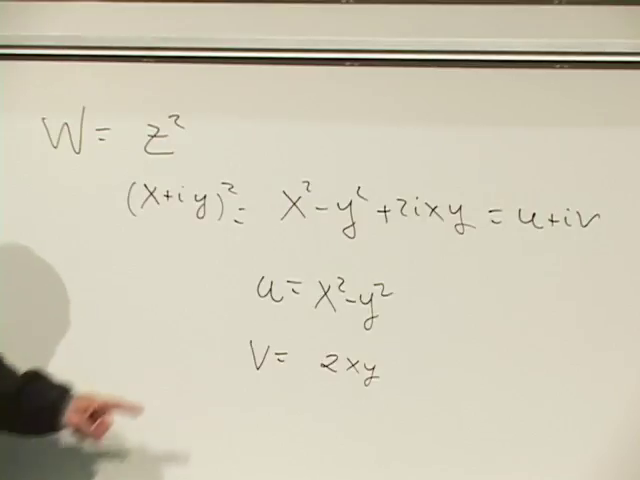
\includegraphics[width=0.68\textwidth]{lecture_08_figure_03.png}
  \caption{Les dérivées mixtes s’annulent ; il reste l’équation de Laplace pour une composante de l’application analytique.}
  \lectureframe{00:23:09}
  \label{fig:l08-harmonic-board}
\end{figure}

On peut aussi donner une interprétation vectorielle. Si
\(\mathbf F=(u,-v)\), les deux équations de Cauchy--Riemann expriment, à un choix d’orientation près, que la divergence et le rotationnel bidimensionnel de \(\mathbf F\) sont tous deux nuls. Nous voici donc revenus à l’électrostatique.

\subsection{Pourquoi les angles sont préservés}

Écrivons deux petits déplacements complexes sous forme polaire :
\begin{equation}
  \delta z=\rho e^{i\theta},
  \qquad
  \Delta z=\rho'e^{i\theta'}.
\end{equation}
La phase de leur rapport est \(\theta-\theta'\), exactement l’angle entre eux. Sous une application analytique,
\begin{equation}
  \frac{\delta w}{\delta z}
  =\frac{\Delta w}{\Delta z}
  =w'(z),
\end{equation}
car la dérivée ne dépend pas de la direction. En réarrangeant, on obtient
\begin{equation}
  \frac{\Delta z}{\delta z}
  =\frac{\Delta w}{\delta w}.
  \label{eq:l08-angle-ratio}
\end{equation}
Les deux membres ont la même phase ; l’angle entre les intervalles initiaux est donc égal à celui entre leurs images.

\begin{figure}[H]
  \centering
  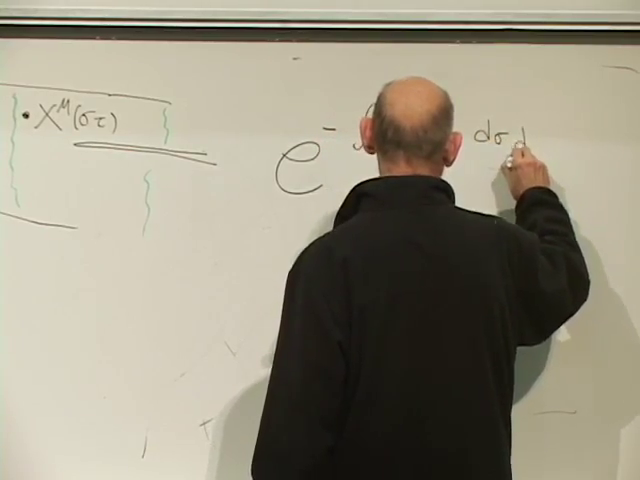
\includegraphics[width=0.70\textwidth]{lecture_08_figure_04.png}
  \medskip

  \begin{tikzpicture}[x=0.9cm,y=0.9cm,>=Latex]
    \begin{scope}
      \draw[->] (-0.2,0) -- (2.3,0);
      \draw[->] (0,-0.2) -- (0,2.1);
      \draw[very thick,blue!65!black,->] (0,0) -- (1.85,0.45)
        node[right] {\(\delta z\)};
      \draw[very thick,orange!75!black,->] (0,0) -- (0.72,1.65)
        node[above] {\(\Delta z\)};
      \draw (0.58,0.14) arc[start angle=14,end angle=66,radius=0.60];
      \node at (1.0,-0.55) {\(z\)-plane};
    \end{scope}
    \draw[->,thick] (3.0,0.9) -- (4.2,0.9)
      node[midway,above] {\(w(z)\)};
    \begin{scope}[xshift=5.0cm]
      \draw[->] (-0.2,0) -- (2.3,0);
      \draw[->] (0,-0.2) -- (0,2.1);
      \draw[very thick,blue!65!black,->] (0,0) -- (1.65,0.70)
        node[right] {\(\delta w\)};
      \draw[very thick,orange!75!black,->] (0,0) -- (0.48,1.62)
        node[above] {\(\Delta w\)};
      \draw (0.54,0.23) arc[start angle=23,end angle=74,radius=0.59];
      \node at (1.0,-0.55) {\(w\)-plane};
    \end{scope}
  \end{tikzpicture}
  \caption{La démonstration au tableau et une reconstruction locale claire. La multiplication par \(w'(z)\) fait tourner et change d’échelle chaque direction infinitésimale de la même façon, préservant ainsi leur angle relatif.}
  \lectureframe{00:34:11}
  \label{fig:l08-angle-proof}
\end{figure}

Ce raisonnement local suppose que \(w'(z)\neq0\). En un point critique, l’application peut ne pas être localement bijective, et la géométrie doit être étudiée séparément. En dehors de ces points, les applications analytiques et les applications conformes qui préservent l’orientation sont localement les mêmes.

\section{Quelques exemples pour exercer l’œil}

\subsection{Carré et conjugaison complexe}

Pour \(w=z^2\),
\begin{equation}
  (x+iy)^2=x^2-y^2+2ixy=u+iv,
\end{equation}
donc
\begin{equation}
  u=x^2-y^2,
  \qquad
  v=2xy.
  \label{eq:l08-z-squared-components}
\end{equation}
Les dérivées secondes de \(u\) sont \(2\) et \(-2\) ; celles de \(v\) s’annulent séparément. Les deux fonctions sont harmoniques, et une dérivation directe vérifie également les équations de Cauchy--Riemann.

\begin{figure}[H]
  \centering
  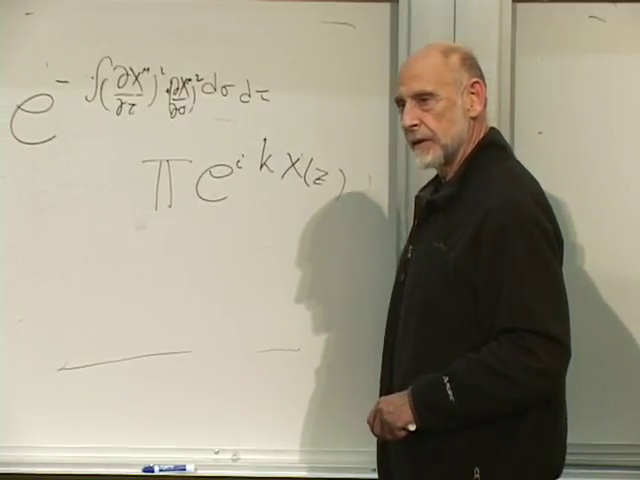
\includegraphics[width=0.72\textwidth]{lecture_08_figure_05.png}
  \caption{L’application qui élève au carré, décomposée en ses composantes harmoniques réelle et imaginaire.}
  \lectureframe{00:36:45}
  \label{fig:l08-z-square-board}
\end{figure}

\begin{classroomqa}
\audiencequestion{La fonction \(1/z\) fournit-elle un exemple non analytique ?
\lecturetimestamp{00:37:49}}
\lecturerresponse{En un seul point. Elle est analytique partout où \(z\neq0\) et possède un pôle à l’origine. Pour voir une application qui échoue partout au test de Cauchy--Riemann, la conjugaison complexe est un meilleur exemple.}
\end{classroomqa}

En revanche,
\begin{equation}
  w=\bar z=x-iy
  \qquad\Longrightarrow\qquad
  u=x,\quad v=-y
\end{equation}
inverse l’orientation. Ses dérivées ne satisfont pas la première équation de Cauchy--Riemann, à cause d’un signe ; cette fonction de \(z\) n’est donc pas analytique.

\begin{figure}[H]
  \centering
  \includegraphics[width=0.62\textwidth]{lecture_08_figure_06.png}
  \caption{La conjugaison complexe constitue le contre-exemple délibérément non analytique.}
  \lectureframe{00:38:38}
  \label{fig:l08-conjugate-board}
\end{figure}

\subsection{L’exponentielle et sa réciproque}

\begin{classroomqa}
\audiencequestion{Si \(e^z\) est analytique, pourquoi son inverse \(\log z\) le serait-elle aussi ? \lecturetimestamp{00:40:38}}
\lecturerresponse{Lorsque l’inverse existe et que \(w'(z)\neq0\), sa dérivée vaut \(1/w'(z)\). L’indépendance par rapport à la direction est donc préservée. À l’échelle globale, le logarithme est multivalué ; on choisit donc une branche et on exclut son point de branchement et sa coupure. L’énoncé conforme local reste valable sur le domaine ainsi choisi.}
\end{classroomqa}

La formule d’Euler donne
\begin{equation}
  w=e^z=e^{x+iy}
  =e^x(\cos y+i\sin y),
\end{equation}
d’où
\begin{equation}
  u=e^x\cos y,
  \qquad
  v=e^x\sin y.
  \label{eq:l08-exponential-components}
\end{equation}
Par exemple,
\(\partial_xu=e^x\cos y=\partial_yv\), et la seconde équation de Cauchy--Riemann se vérifie tout aussi directement.

\begin{figure}[H]
  \centering
  \includegraphics[width=0.68\textwidth]{lecture_08_figure_07.png}
  \caption{Les composantes réelle et imaginaire de l’application exponentielle.}
  \lectureframe{00:42:23}
  \label{fig:l08-exponential-board}
\end{figure}

\section{Demi-plan, bande, cylindre et disque}

\subsection{Le logarithme transforme le rayon en temps}

Considérons le demi-plan droit, où
\(-\pi/2<\theta<\pi/2\), et écrivons
\begin{equation}
  z=re^{i\theta},
  \qquad
  w=\log z=\log r+i\theta.
  \label{eq:l08-log-map}
\end{equation}
Le demi-plan est envoyé sur la bande infinie
\begin{equation}
  -\frac{\pi}{2}<\operatorname{Im}w<\frac{\pi}{2}.
\end{equation}
Les demi-droites de \(\theta\) constant deviennent des droites horizontales, tandis que les demi-cercles de \(r\) constant deviennent des droites verticales. L’origine est envoyée sur \(\operatorname{Re}w=-\infty\), et \(r=\infty\) sur \(\operatorname{Re}w=+\infty\).

\begin{figure}[H]
  \centering
  \includegraphics[width=0.75\textwidth]{lecture_08_figure_08.png}
  \caption{Le logarithme envoie le demi-plan droit sur une bande infinie : les demi-droites polaires et les demi-cercles deviennent une grille rectangulaire orthogonale.}
  \lectureframe{00:47:48}
  \label{fig:l08-log-strip-board}
\end{figure}

La bande est la surface d’univers standard d’une corde ouverte. Sa coordonnée bornée paramètre la position le long de la corde, tandis que la translation dans la direction non bornée correspond au temps de la surface d’univers. Par l’application exponentielle inverse, une translation dans le temps devient une dilatation \(z\mapsto e^a z\). Ainsi, la même symétrie prend la forme d’une translation dans la bande et d’une expansion uniforme dans le demi-plan.

\begin{classroomqa}
\audiencequestion{Où va un point particulier, par exemple \(r=1\), et les coordonnées de la bande sont-elles encore polaires ? \lecturetimestamp{00:50:58}}
\lecturerresponse{Un cercle de rayon fixe devient une droite verticale en \(\operatorname{Re}w=\log r\) ; en particulier, \(r=1\) est envoyé sur la droite centrale \(\operatorname{Re}w=0\). Les coordonnées polaires décrivent le plan \(z\). Le plan \(w\) utilise des coordonnées cartésiennes ordinaires \((\log r,\theta)\).}
\end{classroomqa}

Si l’on applique \(\log z\) au plan privé de l’origine tout entier, la coordonnée angulaire est périodique de \(2\pi\). La bande obtenue a donc ses bords supérieur et inférieur identifiés : c’est un cylindre infini. Le demi-plan avec son bord décrit la surface d’univers d’une corde ouverte ; le plan entier, sans bord et avec un angle périodique, décrit un cylindre de corde fermée.

\begin{figure}[H]
  \centering
  \includegraphics[width=0.75\textwidth]{lecture_08_figure_09.png}
  \caption{La représentation du demi-plan en bande et l’identification périodique qui transforme le plan privé de l’origine en un cylindre de corde fermée.}
  \lectureframe{00:54:23}
  \label{fig:l08-open-closed-board}
\end{figure}

\subsection{Une application de Cayley vers le disque unité}

Une transformation homographique, ou transformation de Möbius, envoie le demi-plan droit sur le disque unité :
\begin{equation}
  w=\frac{z-1}{z+1}.
  \label{eq:l08-cayley}
\end{equation}
Elle envoie \(z=0\) sur \(-1\), \(z=\infty\) sur \(+1\), et l’axe imaginaire sur \(|w|=1\). Si \(z=ir\),
\begin{equation}
  \left|\frac{ir-1}{ir+1}\right|=1.
\end{equation}
Les points tels que \(\operatorname{Re}z>0\) se trouvent à l’intérieur du cercle ; le demi-plan gauche est envoyé à l’extérieur.
\editorialnote{Lors de la dérivation au tableau, on écrit l’inverse \((z+1)/(z-1)\) alors qu’on décrit l’image intérieure du disque. Cet inverse a le même cercle unité pour frontière, mais envoie le demi-plan droit à l’extérieur. L’équation \eqref{eq:l08-cayley} correspond à la convention de l’intérieur du disque, cohérente avec la géométrie énoncée.}

\begin{figure}[H]
  \centering
  \includegraphics[width=0.72\textwidth]{lecture_08_figure_10.png}
  \caption{Construction homographique de la frontière du cercle unité. La convention réciproque visible au tableau échange l’intérieur et l’extérieur.}
  \lectureframe{00:58:38}
  \label{fig:l08-cayley-board}
\end{figure}

Les transformations de Möbius envoient l’ensemble généralisé des cercles et des droites sur des cercles et des droites. La grille radiale et circulaire du demi-plan devient donc deux familles orthogonales d’arcs dans le disque. Un diamètre droit est simplement le cas limite d’un cercle dont le centre est rejeté à l’infini.

\begin{classroomqa}
\audiencequestion{Les arcs tracés à l’intérieur du disque sont-ils vraiment des cercles ?
\lecturetimestamp{01:00:55}}
\lecturerresponse{Oui. Leurs centres se trouvent à des endroits différents, souvent à l’extérieur du disque visible. Le diamètre est la limite de rayon infini de cette même famille.}
\end{classroomqa}

\begin{classroomqa}
\audiencequestion{Le dessin du disque signifie-t-il qu’il s’agit d’une sphère, et où va l’autre demi-plan ? \lecturetimestamp{01:01:21}}
\lecturerresponse{Le dessin présenté ici est un disque plat, pas une sphère. Le demi-plan droit est envoyé à l’intérieur de son bord et le demi-plan gauche à l’extérieur. Si l’on ajoute le point à l’infini au plan complexe tout entier, ce plan étendu peut être représenté par une sphère au moyen d’une projection stéréographique ; c’est un énoncé global différent.}
\end{classroomqa}

\begin{classroomqa}
\audiencequestion{Quelles courbes du disque correspondent aux rayons et aux demi-cercles de rayon constant du plan initial ? \lecturetimestamp{01:02:59}}
\lecturerresponse{L’axe réel positif devient le diamètre reliant \(-1\) et \(+1\). Les autres demi-droites deviennent des arcs de cercle reliant ces mêmes points du bord. Les demi-cercles de rayon fixe deviennent la famille orthogonale qui rejoint le cercle unité en deux points.}
\end{classroomqa}

\begin{figure}[H]
  \centering
  \includegraphics[width=0.72\textwidth]{lecture_08_figure_11.png}
  \caption{Dans le demi-plan, les droites et les demi-cercles deviennent dans le disque des familles orthogonales de cercles et de droites.}
  \lectureframe{01:03:48}
  \label{fig:l08-circle-grid-board}
\end{figure}

\section{La surface d’univers à quatre cordes}

Nous pouvons maintenant revenir à la diffusion. Deux cordes ouvertes entrent, s’unissent en une seule, se propagent pendant un intervalle quelconque, puis se séparent en deux cordes sortantes. En coordonnées de bande, la surface d’univers ressemble à un long ruban fendu à chaque extrémité---— l’image du « pansement sportif ». La durée de vie de l’état intermédiaire n’est pas fixée à l’avance. Elle fait partie des histoires sur lesquelles on intègre l’amplitude.

Soient \((\sigma,\tau)\) les coordonnées sur la surface d’univers, et soit
\begin{equation}
  X^\mu=X^\mu(\sigma,\tau)
  \label{eq:l08-embedding}
\end{equation}
sa position dans l’espace-temps. Les indices \(\sigma,\tau\) désignent les coordonnées sur la surface paramétrique bidimensionnelle ; l’indice \(\mu\) désigne les coordonnées d’espace-temps. Dans la théorie bosonique, \(\mu=0,\ldots,25\) ; dans le cas des supercordes, l’espace-temps compte dix coordonnées.

Après rotation de Wick, les champs d’immersion libres ont pour action euclidienne
\begin{equation}
  S_E[X]
  =\frac{1}{4\pi\alpha'}\int_\Sigma d\sigma\,d\tau\,
  \left[
    \partial_\tau X^\mu\partial_\tau X_\mu
    +\partial_\sigma X^\mu\partial_\sigma X_\mu
  \right].
  \label{eq:l08-euclidean-action}
\end{equation}
L’intégrale de chemin correspondante somme sur toutes les immersions de la surface d’univers choisie dans l’espace-temps :
\begin{equation}
  \int\mathcal D X\,e^{-S_E[X]}.
  \label{eq:l08-bare-worldsheet-integral}
\end{equation}

\begin{figure}[H]
  \centering
  \includegraphics[width=0.74\textwidth]{lecture_08_figure_12.png}
  \caption{Le poids euclidien positif complet de la surface d’univers. Les deux termes en dérivées sont sommés sur toutes les composantes d’espace-temps.}
  \lectureframe{01:11:34}
  \label{fig:l08-action-board}
\end{figure}

La bande fendue possède un bord connexe. La liberté conforme permet donc de la représenter par un disque. Les quatre extrémités éloignées des bandes deviennent quatre points marqués sur le bord. Déplacer ces points modifie la séparation apparente entre la réunion et la séparation dans les coordonnées de bande, mais ne change ni la surface sous-jacente ni la physique.

\begin{figure}[H]
  \centering
  \includegraphics[width=0.76\textwidth]{lecture_08_figure_13.png}
  \caption{La surface d’univers en bande fendue et sa représentation sur un disque, avec les points du bord associés aux cordes externes.}
  \lectureframe{01:15:18}
  \label{fig:l08-bandage-disc-board}
\end{figure}

Les lignes de la grille détaillée utilisées pour représenter cette application conforme n’ont pas de signification physique. Ce qui importe, c’est la topologie, le bord et les points externes marqués. On peut étirer la même surface d’univers pour obtenir différentes représentations selon le canal, sans introduire de nouvelle interaction.

\section{États externes sous forme d’insertions au bord}

L’intégrale sans insertions \eqref{eq:l08-bare-worldsheet-integral} n’indique pas encore quelles quantités de mouvement entrent et sortent. Pour un état scalaire de corde ouverte de quantité de mouvement \(k_i^\mu\), insérons sur le bord l’opérateur vertex
\begin{equation}
  V_i(z_i)=e^{\,i k_i\cdot X(z_i)},
  \qquad
  k_i\cdot X=k_{i\mu}X^\mu.
  \label{eq:l08-vertex}
\end{equation}
Le point \(z_i\) est une position sur le bord de la surface d’univers. Ce n’est ni une coordonnée d’espace-temps ni une direction de quantité de mouvement.

\begin{figure}[H]
  \centering
  \includegraphics[width=0.72\textwidth]{lecture_08_figure_14.png}
  \caption{Le poids euclidien dans le volume et le produit des insertions de quantité de mouvement au bord sont représentés comme des facteurs distincts.}
  \lectureframe{01:18:58}
  \label{fig:l08-vertex-board}
\end{figure}

Pour \(n\) cordes ouvertes externes, la prescription schématique est
\begin{equation}
  \begin{aligned}
    \mathcal A_n(k_1,\ldots,k_n)
    &=\int_{\mathcal M_{0,n}^{\partial}}\!d\mu(z_i)
      \int\mathcal D X\\
    &\quad\times e^{-S_E[X]}
      \prod_{i=1}^{n}e^{\,i k_i\cdot X(z_i)}.
  \end{aligned}
  \label{eq:l08-open-string-prescription}
\end{equation}
L’intégrale fonctionnelle porte sur les immersions \(X^\mu\). L’intégrale de dimension finie porte sur les positions d’insertion non équivalentes au bord. À ce stade, les facteurs de polarisation et la mesure de fixation de jauge sont omis, comme dans le cours.
\editorialnote{Une amplitude de corde complètement fixée en jauge comprend également la contribution de fantômes appropriée, les facteurs de vertex dépendant de l’état, les constantes de couplage et la normalisation. L’équation
\eqref{eq:l08-open-string-prescription} décrit la dépendance envers les champs d’immersion et leurs positions, développée dans ce cours.}

\begin{classroomqa}
\audiencequestion{Si les quantités de mouvement externes sont fixées, pourquoi les intègre-t-on ? \lecturetimestamp{01:20:42}}
\lecturerresponse{On ne les intègre pas. Les \(k_i\) sont des étiquettes fixées de l’amplitude de diffusion. On intègre sur les champs d’immersion et sur les positions \(z_i\) de la surface d’univers où ces quantités de mouvement fixées sont insérées. Cette dernière intégrale remplace celle sur la durée de propagation de la représentation en bande.}
\end{classroomqa}

\begin{classroomqa}
\audiencequestion{Le produit des facteurs de vertex se trouve-t-il dans l’intégrale de chemin, et fait-il partie de l’action ? \lecturetimestamp{01:21:39}}
\lecturerresponse{Il multiplie \(e^{-S_E}\) dans l’intégrale fonctionnelle. On peut aussi exponentier ces facteurs et les considérer comme des termes de source localisés ajoutés à l’action, mais conceptuellement, ce sont des opérateurs vertex, et non des termes de l’action libre dans le volume.}
\end{classroomqa}

\begin{figure}[H]
  \centering
  \includegraphics[width=0.76\textwidth]{lecture_08_figure_15.png}
  \caption{L’intégrale de chemin écrite avec des facteurs séparés \(e^{ik_i\cdot X(z_i)}\) pour les particules externes successives.}
  \lectureframe{01:23:23}
  \label{fig:l08-full-prescription-board}
\end{figure}

\begin{classroomqa}
\audiencequestion{Pourquoi \(e^{ik\cdot X}\) contient-il encore \(i\) après la rotation de Wick de la surface d’univers ? \lecturetimestamp{01:23:42}}
\lecturerresponse{La rotation transforme le temps de la surface d’univers et fait passer le poids dans le volume de \(e^{iS}\) à \(e^{-S_E}\). Le \(i\) dans une fonction propre de quantité de mouvement est la phase de Fourier qui étiquette la quantité de mouvement d’espace-temps. Il joue un autre rôle et demeure donc présent.}
\end{classroomqa}

\begin{classroomqa}
\audiencequestion{La position \(z_i\) détermine-t-elle la direction du vecteur quantité de mouvement ? \lecturetimestamp{01:24:19}}
\lecturerresponse{Non. La direction est encodée dans les composantes d’espace-temps \(k_i^\mu\). Le point d’insertion \(z_i\) indique où cette quantité de mouvement entre dans la description de la surface d’univers ; \(X^\mu(z_i)\) fait partie des valeurs du champ sur lesquelles on somme dans \(\mathcal D X\).}
\end{classroomqa}

\begin{classroomqa}
\audiencequestion{Les angles dessinés entre les branches du pansement représentent-ils les directions des quantités de mouvement physiques ? \lecturetimestamp{01:25:07}}
\lecturerresponse{Non. Le pansement représente l’espace des paramètres, pas une image de la corde dans l’espace-temps physique. On peut dessiner ses branches horizontalement, inclinées ou déformées conformément. Les directions physiques sont portées par les composantes \(k^\mu\), tandis que \(X^\mu(\sigma,\tau)\) est intégrée.}
\end{classroomqa}

\section{L’intégrale gaussienne comme problème d’électrostatique}

L’action \eqref{eq:l08-euclidean-action} est quadratique en chaque composante \(X^\mu\), et les insertions constituent des sources linéaires dès qu’on combine leurs exponentielles à l’action. L’intégrale fonctionnelle est donc gaussienne. Au point selle, chaque composante d’espace-temps satisfait une équation de Poisson de la forme schématique
\begin{equation}
  \nabla^2 X^\mu(z)
  \propto
  i\alpha'\sum_i k_i^\mu\,\delta(z-z_i),
  \label{eq:l08-electrostatic-source}
\end{equation}
avec la condition aux limites de la corde ouverte sur le bord du disque. Chaque \(X^\mu\) se comporte comme un potentiel électrostatique indépendant, et chaque composante de quantité de mouvement \(k_i^\mu\) comme la charge correspondante placée en \(z_i\).

\begin{figure}[H]
  \centering
  \includegraphics[width=0.76\textwidth]{lecture_08_figure_16.png}
  \caption{Le disque avec des sources au bord se lit comme un problème électrostatique bidimensionnel indépendant pour chaque composante d’espace-temps.}
  \lectureframe{01:28:58}
  \label{fig:l08-electrostatic-disc-board}
\end{figure}

Résolvons le problème électrostatique, calculons son énergie, exponentions l’opposé de cette énergie, puis intégrons sur les positions non équivalentes des charges. Avec la normalisation standard des cordes ouvertes, le corrélateur des champs d’immersion fournit le facteur de Koba--Nielsen
\begin{equation}
  \left\langle\prod_i e^{\,ik_i\cdot X(z_i)}\right\rangle
  \propto
  (2\pi)^D\delta^{(D)}\!\left(\sum_i k_i\right)
  \prod_{i<j}|z_i-z_j|^{2\alpha' k_i\cdot k_j}.
  \label{eq:l08-koba-nielsen}
\end{equation}
La fonction delta exprime la conservation de la quantité de mouvement. Le produit contient les énergies électrostatiques par paires. Pour les quatre insertions scalaires au bord considérées ici, fixer trois positions transforme l’intégrale restante en l’intégrale bêta d’Euler rencontrée dans les cours précédents.

\begin{classroomqa}
\audiencequestion{Y a-t-il vingt-six énergies électrostatiques ou une seule ?
\lecturetimestamp{01:30:53}}
\lecturerresponse{Il existe un potentiel et un champ indépendants pour chaque composante d’espace-temps. Dans une base orthonormée de l’espace cible, leurs énergies quadratiques ne comportent pas de termes croisés ; leurs contributions s’additionnent en une action totale avant l’exponentiation.}
\end{classroomqa}

\begin{classroomqa}
\audiencequestion{La coordonnée angulaire du disque est-elle l’angle de diffusion physique ? \lecturetimestamp{01:32:10}}
\lecturerresponse{Non. C’est un paramètre de position sur la surface d’univers. Sa combinaison non équivalente est reliée à l’intervalle de propagation intermédiaire et fait l’objet d’une intégration. L’angle de diffusion physique est encodé dans des invariants de Lorentz construits à partir des quantités de mouvement fixées.}
\end{classroomqa}

\begin{classroomqa}
\audiencequestion{Pourquoi cette construction échoue-t-elle hors de la dimension critique ? \lecturetimestamp{01:32:35}}
\lecturerresponse{Les seules intégrales gaussiennes formelles ne constituent pas toute la condition de cohérence. La fixation de jauge introduit une anomalie conforme, dont les contributions de matière et de fantômes ne s’annulent qu’à la dimension critique : \(D=26\) pour la corde bosonique et \(D=10\) pour la supercorde. Sans cette annulation, la symétrie conforme supposée de la surface d’univers quantique est perdue.}
\end{classroomqa}

\begin{classroomqa}
\audiencequestion{Avons-nous déjà supposé trois grandes dimensions spatiales et des dimensions supplémentaires compactifiées ? \lecturetimestamp{01:33:38}}
\lecturerresponse{Non. La compactification n’intervient pas encore dans la construction. À ce stade, les coordonnées bosoniques parcourent toujours les vingt-six directions de l’espace cible, ou les dix directions dans le cas de la supercorde. La question de savoir comment certaines peuvent rester macroscopiquement grandes sera abordée dans la discussion suivante.}
\end{classroomqa}

\begin{classroomqa}
\audiencequestion{Le lien avec l’électrostatique tient-il simplement au fait que les coordonnées satisfont l’équation de Laplace ? \lecturetimestamp{01:33:57}}
\lecturerresponse{Exactement. En dehors des points d’insertion, chaque \(X^\mu\) est harmonique ; les opérateurs vertex fournissent des sources en delta de Dirac. C’est mathématiquement le même problème aux limites qu’un potentiel statique bidimensionnel avec des charges ponctuelles, que l’on emploie ou non le vocabulaire de l’électrostatique.}
\end{classroomqa}

\subsection{Redondance conforme et nombre de modules}

Le disque possède un groupe d’automorphismes conformes à trois paramètres réels, \(\mathrm{PSL}(2,\mathbb R)\). On peut donc fixer trois points ordonnés du bord à des positions choisies par commodité. Pour quatre cordes externes, il ne reste qu’à intégrer sur la position du quatrième point ; pour \(n\) insertions ordonnées au bord, il reste
\begin{equation}
  n-3
  \label{eq:l08-n-minus-three}
\end{equation}
intégrales réelles sur les positions au niveau arbre.

\begin{classroomqa}
\audiencequestion{Existe-t-il quatre positions angulaires indépendantes autour du disque ? \lecturetimestamp{01:34:37}}
\lecturerresponse{Pas du point de vue physique. On écrit d’abord quatre positions, mais la symétrie conforme du disque permet de placer les trois premières où l’on veut. Seule subsiste la position relative de la quatrième pour l’amplitude à deux cordes entrantes et deux cordes sortantes.}
\end{classroomqa}

\begin{figure}[H]
  \centering
  \includegraphics[width=0.72\textwidth]{lecture_08_figure_17.png}
  \caption{Quatre insertions au bord du disque. La liberté conforme permet d’en fixer trois, ce qui laisse un module pour le processus à quatre points.}
  \lectureframe{01:35:18}
  \label{fig:l08-fix-three-board}
\end{figure}

\begin{classroomqa}
\audiencequestion{Que se passe-t-il si les deux points de séparation ne sont pas à la même hauteur dans le dessin de la bande ? \lecturetimestamp{01:35:24}}
\lecturerresponse{Une application conforme peut supprimer ce décalage apparent. Les dessins différents sont des représentations coordonnées d’un même module. L’intégrale invariante porte sur la position restante au bord, ou, de façon équivalente, sur l’intervalle de propagation.}
\end{classroomqa}

\begin{classroomqa}
\audiencequestion{Pour un plus grand nombre de particules externes, combien de paramètres de position restent-ils ? \lecturetimestamp{01:36:00}}
\lecturerresponse{Fixons trois points d’insertion par symétrie conforme et intégrons sur les \(n-3\) autres. C’est le décompte des modules de bord pour une amplitude de corde ouverte ordonnée au niveau arbre.}
\end{classroomqa}

\begin{classroomqa}
\audiencequestion{Quel est le lien avec la théorie M ?
\lecturetimestamp{01:36:37}}
\lecturerresponse{Pas encore. La construction présentée ici concerne la diffusion perturbative de cordes ouvertes sur une surface d’univers. Le lien avec la théorie M exige des idées de dualité et des idées non perturbatives qui seront abordées plus tard ; la question est donc explicitement reportée.}
\end{classroomqa}

\begin{classroomqa}
\audiencequestion{Une bande verticale ou croisée différente correspond-elle à un calcul différent ? \lecturetimestamp{01:36:49}}
\lecturerresponse{Non. On peut fixer un point commode et laisser le module restant parcourir tout son intervalle. Les représentations en bandes et l’intégrale sur les positions des points du bord du disque correspondent à des découpages différents d’une même intégrale ; c’est pourquoi toutes les cordes externes peuvent être traitées de manière symétrique.}
\end{classroomqa}

\section{Ce que la prescription ne résout pas encore}

La formule sur le disque s’étend immédiatement à un plus grand nombre de cordes externes : on ajoute des opérateurs vertex et on intègre sur leurs \(n-3\) positions distinctes sur le bord. Elle constitue une prescription précise au niveau de l’arbre pour un modèle de cordes cohérent, mais ne fournit pas encore un modèle réaliste de la physique des particules observée. La théorie bosonique simple a la mauvaise dimension d’espace-temps et présente d’autres défauts physiques. Les supercordes améliorent le spectre et abaissent la dimension critique à dix, mais il reste à compactifier six dimensions spatiales.

\begin{classroomqa}
\audiencequestion{Ce modèle simple est-il déjà en accord avec les expériences de collision de particules ? \lecturetimestamp{01:39:06}}
\lecturerresponse{Non. La structure des résonances rappelle historiquement la diffusion hadronique, mais le modèle bosonique à vingt-six dimensions ne peut pas décrire directement les particules observées. Le formalisme définit des amplitudes de diffusion pour ce modèle ; pour retrouver la nature, il faut un spectre réaliste, une compactification, des interactions et un choix du vide.}
\end{classroomqa}

\begin{classroomqa}
\audiencequestion{La compactification réduira-t-elle le nombre de dimensions supplémentaires et produira-t-elle des données réalistes sur les particules ? \lecturetimestamp{01:41:10}}
\lecturerresponse{Elle peut réduire la dimension macroscopique effective et engendrer des spectres de particules ainsi que des groupes de jauge. C’est aussi là qu’intervient une grande partie de la difficulté mathématique réelle. On connaît de nombreuses compactifications cohérentes, et le choix d’un modèle unique des particules élémentaires observées demeure un problème non résolu.}
\end{classroomqa}

Le cours insiste sur cette distinction au lieu de présenter une théorie achevée. Les constructions de cordes sont mathématiquement bien définies et ont apporté des résultats profonds sur la gravité et la géométrie, mais leur multiplicité fait elle-même partie du problème physique.

\begin{classroomqa}
\audiencequestion{Existe-t-il un moyen simple de retenir pourquoi la dimension critique bosonique vaut vingt-six ? \lecturetimestamp{01:43:19}}
\lecturerresponse{Le calcul antérieur des oscillateurs utilisait la somme régularisée des énergies du point zéro \(1+2+3+\cdots=-1/12\). La contribution des oscillateurs transverses fait intervenir vingt-quatre directions ; en rétablissant les deux coordonnées longitudinales de l’espace-temps, on obtient \(24+2=26\). C’est un moyen mnémotechnique pour se rappeler l’argument de cohérence précédent, et non une nouvelle démonstration.}
\end{classroomqa}

\begin{classroomqa}
\audiencequestion{Les impulsions insérées \(k_i\) sont-elles elles-mêmes quantifiées ?
\lecturetimestamp{01:43:46}}
\lecturerresponse{Dans un espace-temps non compact, leurs composantes sont continues. Ce qui est quantifié, c’est le niveau des oscillateurs et, par conséquent, le spectre autorisé des masses au carré. Les dimensions compactes peuvent quantifier les composantes correspondantes de quantité de mouvement et d’enroulement, mais cela relève de la discussion suivante.}
\end{classroomqa}

\chapter{Cordes, gravité, compactification et T-dualité}

\lectureoverview{Une particule ponctuelle peut se déplacer de façon cohérente sur presque toute géométrie lisse, mais ce n’est pas le cas d’une corde quantique. Ses oscillations de point zéro, en nombre infini, sondent l’espace cible à des échelles toujours plus courtes, et la géométrie effective change à mesure que ces oscillations sont rétablies. Exiger que ce processus atteigne un point fixe conduit à \(R_{\mu\nu}=0\), l’équation d’Einstein dans le vide. Nous passons ensuite de cette condition de cohérence à la compactification. Un cercle fournit à la fois des états de quantité de mouvement de Kaluza--Klein et des états d’enroulement de la corde ; leur échange identifie un cercle de rayon \(R\) à un cercle de rayon \(\alpha'/R\).}

\section{La cohérence comme principe de sélection}

Deux questions se posent. Pourquoi la gravité apparaît-elle dans la théorie des cordes, et pourquoi celle-ci est-elle beaucoup moins permissive que la mécanique des particules ponctuelles ? En réalité, ces deux questions n’en font qu’une. Une géométrie de fond n’est acceptable que si une corde peut s’y propager sans que la théorie conserve une dépendance arbitraire à la finesse avec laquelle nous la résolvons.

Commençons par le problème de référence : une particule ponctuelle contrainte à se déplacer sur une surface courbe lisse. Classiquement, elle suit une géodésique, l’analogue intrinsèque d’une ligne droite. On peut approximer le mouvement par une succession de petits segments, écrire une équation aux différences, puis faire tendre la longueur des segments vers zéro. On obtient ainsi une équation différentielle ordinaire dont la limite continue est bien définie.

La mécanique quantique modifie la somme sur les histoires, mais pas la conclusion. Au lieu de sélectionner une trajectoire classique, on somme les amplitudes associées aux trajectoires sur la surface. On peut de nouveau découper le temps en petits intervalles ; la limite se décrit de façon équivalente par une équation de Schr\"odinger sur l’espace des configurations courbe. Pour une surface lisse, la limite donne un propagateur et un spectre bien définis.

\begin{figure}[H]
  \centering
  \includegraphics[width=0.72\textwidth]{lecture_09_figure_01.png}
  \caption{Une trajectoire lisse sur la surface et une trajectoire en zigzag issue de la somme quantique découpée en tranches temporelles. Toutes deux restent intrinsèques à la surface cible.}
  \lectureframe{00:05:10}
  \label{fig:l09-particle-paths}
\end{figure}

\begin{classroomqa}
\audiencequestion{Dans l’intégrale de chemin, toutes les trajectoires doivent-elles rester sur la surface ? \lecturetimestamp{00:05:39}}
\lecturerresponse{Oui. La surface est l’espace des configurations de la particule, et non une feuille plongée dans un espace plus vaste que la particule pourrait traverser en prenant un raccourci. Chaque point intermédiaire appartient à la surface, et toutes les longueurs et toutes les actions sont calculées à l’aide de sa métrique intrinsèque.}
\end{classroomqa}

La question correspondante pour une corde est plus difficile. Une corde n’est pas caractérisée uniquement par la position de son centre de masse. Elle porte une tour infinie d’oscillateurs ; améliorer la résolution revient donc à admettre davantage de degrés de liberté dynamiques. La théorie n’est cohérente que si les observables tendent vers une limite lorsque cette tour est rétablie.

\section{La particule ponctuelle sur une sphère}

La sphère est la géométrie courbe la plus simple pour effectuer un test. Soit une sphère de rayon \(R\), sur laquelle nous plaçons d’abord une particule de masse \(m\). Pour un mouvement le long d’un grand cercle,
\begin{equation}
  E=\frac{1}{2}mv^2=\frac{p^2}{2m},
  \qquad
  L=pR.
  \label{eq:l09-particle-energy}
\end{equation}
Par conséquent,
\begin{equation}
  E=\frac{L^2}{2mR^2}
   =\frac{L^2}{2I},
  \qquad
  I=mR^2.
  \label{eq:l09-rotor-energy}
\end{equation}
Le rayon intervient par l’intermédiaire du moment d’inertie. La quantification du moment cinétique donne le spectre familier du rotor rigide, sans aucune dépendance à l’égard d’un cutoff ultraviolet.

\begin{figure}[H]
  \centering
  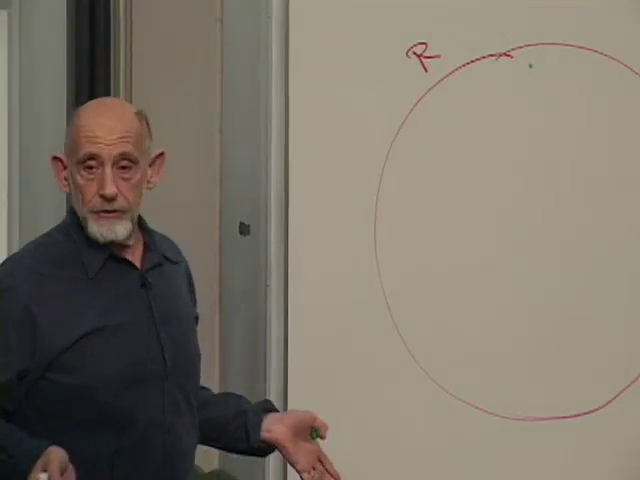
\includegraphics[width=0.74\textwidth]{lecture_09_figure_02.png}
  \caption{Le calcul de référence pour la particule ponctuelle : \(p^2/(2m)=L^2/(2mR^2)=L^2/(2I)\).}
  \lectureframe{00:11:25}
  \label{fig:l09-sphere-rotor}
\end{figure}

Cet exemple sans difficulté est important. La courbure en elle-même n’est pas le problème. Celui-ci apparaît lorsque la courbure est couplée à l’extension quantique interne d’une corde.

\section{La corde du vide n’est pas ponctuelle}

Considérons une coordonnée transverse d’une corde ouverte et soustrayons son centre de masse. Le développement en oscillateurs utilisé ici est schématique :
\begin{equation}
  X(\sigma)-X_{\mathrm{cm}}
  \sim
  \sum_{n=1}^{\infty}
  \frac{a_n+a_n^\dagger}{\sqrt n}\cos(n\sigma).
  \label{eq:l09-mode-expansion}
\end{equation}
Les éléments essentiels sont les modes cosinus, les opérateurs d’oscillateur et le facteur \(1/\sqrt n\). Les normalisations exactes n’interviennent pas dans l’argument sur la taille.
\editorialnote{Le développement précis comporte des facteurs de \(\alpha'\) dépendant des conventions, des constantes numériques et un choix de notation pour les oscillateurs. L’équation \eqref{eq:l09-mode-expansion} ne conserve que la dépendance nécessaire à l’estimation ultraviolette, comme dans le calcul au tableau.}

\begin{figure}[H]
  \centering
  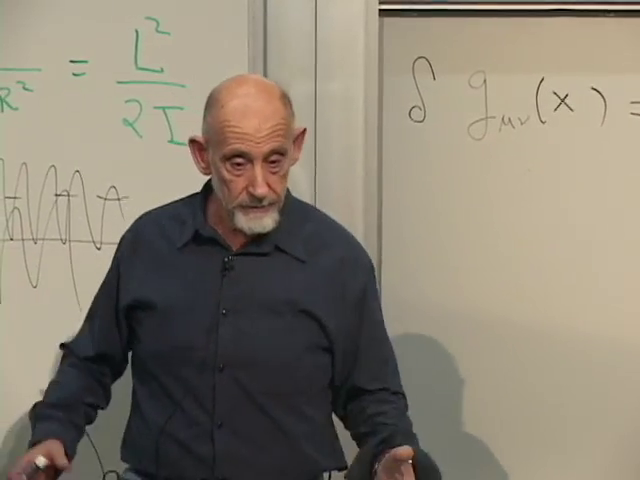
\includegraphics[width=0.78\textwidth]{lecture_09_figure_03.png}
  \caption{Le développement structurel en oscillateurs et la double somme obtenue en l’élevant au carré.}
  \lectureframe{00:15:20}
  \label{fig:l09-string-modes}
\end{figure}

La distance au carré au centre de masse, dans le vide des oscillateurs, vaut
\begin{align}
  \expect{\bigl(X(\sigma)-X_{\mathrm{cm}}\bigr)^2}_0
  &\sim
  \sum_{n,m\geq1}
  \frac{\cos(n\sigma)\cos(m\sigma)}{\sqrt{nm}}\notag\\
  &\qquad\times
  \bra{0}(a_n+a_n^\dagger)\notag\\
  &\hspace{6em}\times(a_m+a_m^\dagger)\ket{0}.
  \label{eq:l09-size-double-sum}
\end{align}
La plupart des termes s’annulent. Deux opérateurs d’annihilation annihilent le ket ; deux opérateurs de création donnent un état orthogonal au bra ; et un opérateur de création suivi d’un opérateur d’annihilation a également une valeur moyenne nulle dans le vide, dans cet ordre. La contraction qui subsiste est
\begin{equation}
  \bra{0}a_n a_m^\dagger\ket{0}=\delta_{nm}.
  \label{eq:l09-vacuum-contraction}
\end{equation}

\begin{figure}[H]
  \centering
  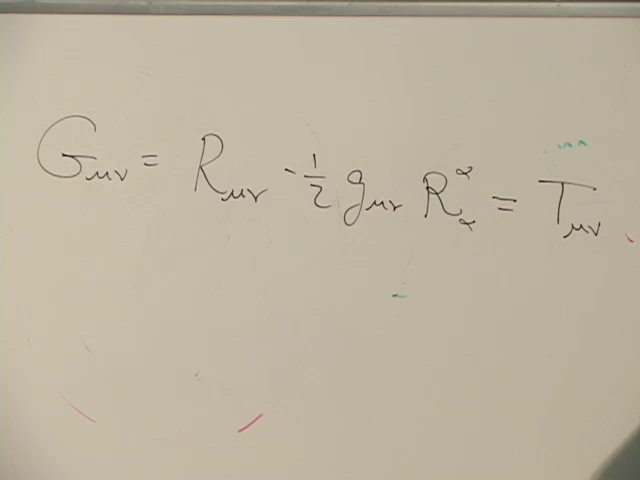
\includegraphics[width=0.74\textwidth]{lecture_09_figure_04.png}
  \caption{La contraction dans le vide qui subsiste réduit la double somme sur les oscillateurs à une somme simple.}
  \lectureframe{00:20:10}
  \label{fig:l09-vacuum-contraction}
\end{figure}

Ainsi,
\begin{equation}
  \expect{\bigl(X(\sigma)-X_{\mathrm{cm}}\bigr)^2}_0
  \sim
  \sum_{n=1}^{\infty}\frac{\cos^2(n\sigma)}{n}.
  \label{eq:l09-size-single-sum}
\end{equation}
En un point générique de la corde, ou après une moyenne sur \(\sigma\), \(\cos^2(n\sigma)\) donne environ \(1/2\). Avec un cutoff sur les modes \(N\),
\begin{equation}
  \expect{\bigl(X-X_{\mathrm{cm}}\bigr)^2}_{0,N}
  \sim
  \frac{1}{2}\sum_{n=1}^{N}\frac{1}{n}
  =\frac{1}{2}\log N+O(1).
  \label{eq:l09-logarithmic-size}
\end{equation}

\begin{figure}[H]
  \centering
  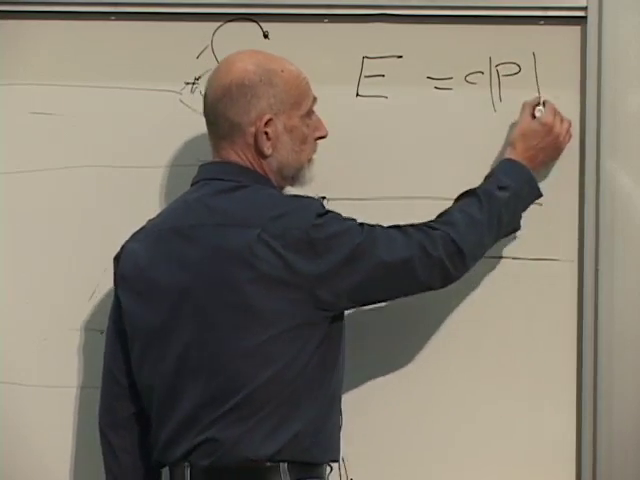
\includegraphics[width=0.72\textwidth]{lecture_09_figure_05.png}
  \caption{Le calcul au tableau aboutit à la somme harmonique qui régit l’étalement de l’état fondamental.}
  \lectureframe{00:22:05}
  \label{fig:l09-harmonic-size}
\end{figure}

En ne conservant, par exemple, que les vingt-cinq premiers modes, on obtient un objet flou de taille finie, mais pas encore la corde continue. La suppression du cutoff fait croître logarithmiquement l’étalement quadratique moyen. Il ne faut pas interpréter cette conclusion comme une preuve de l’incohérence de la théorie des cordes en espace plat. En espace plat, le mouvement du centre de masse et celui des oscillateurs se séparent, et de délicates compensations dans les amplitudes physiques préservent la localité attendue. La croissance de la taille est un signal d’alerte. La courbure nous indique si ce signal annonce une défaillance.

\section{Quand l’étalement interne modifie la géométrie}

Plaçons la corde près du pôle Nord de la sphère. Lorsque tous les oscillateurs sont éteints, elle se comporte comme la particule ponctuelle que nous venons d’étudier. À mesure que l’on admet des modes de plus haute fréquence, la corde devient un enchevêtrement fluctuant qui s’étale sur la calotte. Son centre peut toujours parcourir la sphère, mais l’objet dont le moment d’inertie intervient dans l’énergie de rotation est maintenant étendu.

Pour un axe passant par le centre de la sphère et ses pôles,
\begin{equation}
  I=\int r_\perp^2\,dm,
  \label{eq:l09-extended-inertia}
\end{equation}
où \(r_\perp\) est la distance perpendiculaire d’un élément de corde à cet axe. Un point situé à l’équateur de l’orbite a le bras de levier pertinent le plus grand. Les portions de corde qui retombent vers l’axe contribuent moins. À masse totale fixée, cela diminue le moment d’inertie effectif :
\begin{equation}
  I_{\mathrm{eff}}<mR^2.
  \label{eq:l09-inertia-reduction}
\end{equation}
L’énergie de rotation ressemble donc à celle d’un objet ponctuel sur une sphère plus petite :
\begin{equation}
  E_{\mathrm{rot}}
  =\frac{L^2}{2I_{\mathrm{eff}}}
  \equiv \frac{L^2}{2mR_{\mathrm{eff}}^2},
  \qquad R_{\mathrm{eff}}<R.
  \label{eq:l09-effective-radius}
\end{equation}

\begin{classroomqa}
\audiencequestion{Pourquoi le moment d’inertie devrait-il tendre vers zéro si la corde s’étale sur une région plus vaste ? \lecturetimestamp{00:33:23}}
\lecturerresponse{Il s’agit ici de la description effective après des coarse-grainings successifs, et non de prétendre que la distribution étendue brute a immédiatement un moment d’inertie nul. La première bande de modes transforme le point en une masse floue qui se comporte comme si elle vivait sur une sphère plus petite. La bande suivante résout la structure à l’intérieur de chacune de ces masses et répète le même processus de renormalisation. La répétition de cette comparaison fait décroître le rayon effectif.}
\end{classroomqa}

\begin{figure}[H]
  \centering
  \includegraphics[width=0.72\textwidth]{lecture_09_figure_06.png}
  \medskip

  \begin{adjustbox}{max width=\linewidth}
  \begin{tikzpicture}[x=1cm,y=1cm,>=Latex]
    \draw[thick] (0,0) circle (2.15);
    \draw[dashed] (0,-2.55) -- (0,2.55);
    \draw[blue!65!black,thick]
      (-0.22,2.05)
      .. controls (-1.22,1.75) and (-1.52,1.08) .. (-1.06,0.44)
      .. controls (-0.55,-0.10) and (0.35,0.02) .. (1.10,0.68)
      .. controls (1.48,1.12) and (1.16,1.80) .. (0.20,2.05);
    \draw[red!70!black,dashed] (0,0) circle (1.25);
    \draw[->] (2.70,1.55) -- (4.05,1.55);
    \node[align=center] at (3.37,1.98) {add shorter\\modes};
    \draw[thick] (6.15,0) circle (1.25);
    \draw[dashed] (6.15,-1.65) -- (6.15,1.65);
    \draw[blue!65!black,thick]
      (6.00,1.18)
      .. controls (5.42,0.88) and (5.46,0.25) .. (6.02,-0.06)
      .. controls (6.46,-0.28) and (6.90,0.45) .. (6.28,1.18);
    \node at (0,-3.00) {sphere of radius \(R\)};
    \node at (6.15,-2.05) {effective radius \(R_{\mathrm{eff}}\)};
  \end{tikzpicture}
  \end{adjustbox}
  \caption{La corde près du pôle Nord dessinée au tableau et une reconstruction claire de l’argument du rayon effectif. Le cercle intérieur en pointillés représente une géométrie effective, et non une seconde coquille physique à l’intérieur de la sphère.}
  \lectureframe{00:35:15}
  \label{fig:l09-shrinking-sphere}
\end{figure}

C’est un énoncé de groupe de renormalisation. Un cutoff fini fait de la corde une masse dont la résolution interne est finie. Augmenter le cutoff modifie la mécanique de cette masse. Sur une sphère à courbure positive, chaque couche de modes ajoutée réduit la taille du fond que l’on déduit du mouvement à grande distance. Si le résultat ne se stabilise jamais, il n’existe pas de théorie des cordes indépendante du cutoff sur ce fond.

\section{La métrique doit atteindre un point fixe}

Remplaçons maintenant la sphère par une métrique générale de l’espace cible \(g_{\mu\nu}(x)\). L’intégration d’une fine couche logarithmique de modes d’oscillateur modifie cette métrique par un tenseur local symétrique de rang deux. Cette variation doit s’annuler en espace plat et commencer par des termes à deux dérivées de la métrique. Au premier ordre, la covariance laisse le tenseur de Ricci comme candidat pertinent :
\begin{equation}
  \frac{\partial g_{\mu\nu}}{\partial\log\Lambda}
  =-C\,R_{\mu\nu}+\cdots ,
  \qquad C>0
  \label{eq:l09-ricci-flow}
\end{equation}
dans le sens du coarse-graining utilisé dans l’argument géométrique. Une courbure positive fait alors décroître le rayon d’une sphère, comme requis.
\editorialnote{La normalisation et le signe dépendent du fait que le paramètre de renormalisation augmente vers l’ultraviolet ou vers l’infrarouge. Dans la notation conventionnelle sur la feuille d’univers, la fonction bêta métrique au premier ordre est \(\beta^g_{\mu\nu}=\alpha'R_{\mu\nu}+\cdots\). L’énoncé invariant utilisé ici est que l’indépendance à l’égard du cutoff exige l’annulation de la fonction bêta et donc, à cet ordre, de \(R_{\mu\nu}\).}

\begin{figure}[H]
  \centering
  \includegraphics[width=0.76\textwidth]{lecture_09_figure_07.png}
  \caption{La variation de la métrique est représentée schématiquement par l’opposé du tenseur de Ricci, avec une courbe d’adoucissement dessinée à côté.}
  \lectureframe{00:43:00}
  \label{fig:l09-ricci-flow-board}
\end{figure}

\begin{classroomqa}
\audiencequestion{Où le cutoff des oscillateurs \(N\) intervient-il dans cette équation d’évolution ? \lecturetimestamp{00:43:38}}
\lecturerresponse{C’est la variable d’échelle. La somme qui détermine la taille de la corde varie logarithmiquement lorsque le mode maximal inclus change ; le paramètre d’évolution naturel est donc \(\log N\), ou, de façon équivalente, \(\log\Lambda\). L’équation \eqref{eq:l09-ricci-flow} décrit la variation infinitésimale due à une couche logarithmique de modes.}
\end{classroomqa}

Un fond admissible est un point fixe de cet écoulement. Au premier ordre,
\begin{equation}
  \boxed{R_{\mu\nu}=0.}
  \label{eq:l09-ricci-flat}
\end{equation}
Ricci-plat ne signifie pas que toutes les composantes du tenseur de Riemann s’annulent. Les ondes gravitationnelles, par exemple, peuvent présenter une courbure non nulle dans le vide tout en vérifiant \(R_{\mu\nu}=0\).

\subsection{La même condition est l’équation d’Einstein dans le vide}

En omettant les constantes conventionnelles, l’équation d’Einstein s’écrit
\begin{equation}
  G_{\mu\nu}
  \equiv
  R_{\mu\nu}-\frac12 g_{\mu\nu}R
  =T_{\mu\nu}.
  \label{eq:l09-einstein}
\end{equation}

\begin{figure}[H]
  \centering
  \includegraphics[width=0.78\textwidth]{lecture_09_figure_08.png}
  \caption{Le tenseur d’Einstein et le tenseur énergie-impulsion au tableau.}
  \lectureframe{00:47:15}
  \label{fig:l09-einstein-board}
\end{figure}

Dans le vide, \(T_{\mu\nu}=0\). En prenant la trace en \(D\) dimensions d’espace-temps, on obtient
\begin{equation}
  0=g^{\mu\nu}G_{\mu\nu}
   =\left(1-\frac{D}{2}\right)R.
  \label{eq:l09-einstein-trace}
\end{equation}
Pour \(D\neq2\), on a \(R=0\), et la substitution dans \eqref{eq:l09-einstein} donne \(R_{\mu\nu}=0\). Ainsi, la condition selon laquelle la corde doit perdre sa dépendance au cutoff est l’équation du champ gravitationnel dans le vide. La gravité n’a pas été ajoutée à la théorie : elle apparaît comme le prix de la cohérence.

Le mot \emph{vide} ne signifie pas qu’il ne se passe rien. Il signifie qu’il n’y a pas de source d’énergie-impulsion dans la région. Les équations de Maxwell sans source admettent des ondes électromagnétiques, et les équations d’Einstein sans source admettent des ondes gravitationnelles. La géométrie peut être dynamique même lorsque son tenseur de Ricci s’annule.

\begin{classroomqa}
\audiencequestion{Cette condition est-elle liée à l’invariance conforme ?
\lecturetimestamp{00:52:20}}
\lecturerresponse{Oui, bien que l’enregistrement ne permette que partiellement de saisir la question. La symétrie pertinente est l’invariance conforme de la théorie quantique sur la \emph{feuille d’univers}. Exiger l’annulation de l’anomalie d’échelle sur la feuille d’univers revient à imposer l’annulation de la fonction bêta métrique. Il ne faut pas confondre cela avec l’exigence d’invariance conforme de l’espace-temps lui-même.}
\end{classroomqa}

Il existe une seconde condition de cohérence. L’invariance conforme sur la feuille d’univers fixe aussi la dimension critique de l’espace-temps : dix pour les supercordes et vingt-six pour la corde bosonique. La platitude de Ricci ne constitue donc pas la liste complète des exigences, mais c’est la condition qui fait apparaître le plus directement l’équation d’Einstein.

\section{Des dimensions compactes plutôt que des dimensions manquantes}

Un fond de supercordes comporte neuf dimensions spatiales et une dimension temporelle. Notre monde macroscopique ne présente que trois grandes directions spatiales ; six dimensions spatiales doivent donc être cachées ou rendues autrement inaccessibles aux échelles ordinaires. La compactification les conserve comme de véritables directions, tout en leur donnant une étendue finie et petite.

\begin{classroomqa}
\audiencequestion{Si différents observateurs ont des horloges différentes, cela revient-il à avoir plus d’une dimension temporelle ? \lecturetimestamp{00:56:59}}
\lecturerresponse{Non. Plusieurs horloges sont plusieurs instruments qui mesurent des coordonnées dans un seul espace-temps ; elles ne créent pas des directions temporelles indépendantes. Les dimensions supplémentaires envisagées ici sont spatiales. Les constructions quantiques et causales usuelles ne fournissent pas de théorie cohérente comparable comportant plusieurs directions temporelles locales ; cette possibilité ne fait donc pas partie de ce modèle de compactification.}
\end{classroomqa}

Imaginons des êtres qui pensent que leur monde est une ligne. À faible résolution, ils ne peuvent se déplacer que vers l’avant ou vers l’arrière. Mais sous un microscope suffisamment puissant, la ligne se révèle être un cylindre très fin. Un petit être peut se déplacer autour de sa direction circulaire autant que le long de sa longueur. Cette seconde direction a toujours été présente ; sa circonférence était trop petite pour que les sondes à faible résolution puissent la distinguer.

\begin{figure}[H]
  \centering
  \includegraphics[width=0.78\textwidth]{lecture_09_figure_09.png}
  \caption{Un cylindre étroit et des trajectoires qui s’enroulent autour de sa direction circulaire cachée.}
  \lectureframe{01:01:00}
  \label{fig:l09-hidden-cylinder}
\end{figure}

On peut représenter un cylindre par une bande dont les bords supérieur et inférieur sont identifiés. Le passage par le bord supérieur ramène au bord inférieur à la même position longitudinale. Aucun des deux bords n’est une frontière physique. On peut effectuer la même opération dans deux directions : identifier les bords gauche et droit d’un rectangle, ainsi que ses bords supérieur et inférieur. On obtient alors un tore à deux dimensions.

\begin{figure}[H]
  \centering
  \includegraphics[width=0.76\textwidth]{lecture_09_figure_10.png}
  \medskip

  \begin{tikzpicture}[x=0.82cm,y=0.82cm,>=Latex]
    \draw[thick] (0,0) rectangle (4,2.15);
    \draw[blue!65!black,->] (0,2.48) -- (4,2.48);
    \draw[blue!65!black,->] (4,-0.34) -- (0,-0.34);
    \node at (2,-0.82) {one periodic direction};
    \draw[thick] (6.1,0) rectangle (10.1,2.15);
    \draw[blue!65!black,->] (6.1,2.48) -- (10.1,2.48);
    \draw[blue!65!black,->] (10.1,-0.34) -- (6.1,-0.34);
    \draw[red!70!black,->] (5.76,0) -- (5.76,2.15);
    \draw[red!70!black,->] (10.44,2.15) -- (10.44,0);
    \node at (8.1,-0.82) {two periodic directions};
  \end{tikzpicture}
  \caption{Le parallélépipède dessiné au tableau et une description claire par domaine fondamental. L’identification d’une paire de bords donne un cylindre ; celle des deux paires donne un tore.}
  \lectureframe{01:04:40}
  \label{fig:l09-periodic-identification}
\end{figure}

Le tore est d’abord un objet topologique, avant d’être une surface en forme de beignet dans l’espace à trois dimensions. Si l’on coupe un tore une fois, il devient un cylindre ; si l’on le coupe une seconde fois, il devient un rectangle, à condition de conserver les identifications de bords. On peut munir ce rectangle d’une métrique plate ; le tore plat ainsi obtenu a une courbure de Riemann localement nulle et est donc bien Ricci-plat.

Une trajectoire droite sur le rectangle se poursuit en ligne droite lorsqu’elle traverse un bord identifié. Si sa pente est le rapport rationnel des deux périodes, elle finit par se refermer. Si ce rapport est irrationnel, elle ne se referme jamais et devient dense sur le tore.

\begin{figure}[H]
  \centering
  \includegraphics[width=0.76\textwidth]{lecture_09_figure_11.png}
  \caption{Dans un domaine fondamental, des segments droits répétés représentent une seule trajectoire ininterrompue sur le tore.}
  \lectureframe{01:11:00}
  \label{fig:l09-torus-trajectory}
\end{figure}

On construit les tores de dimension supérieure de la même façon. Un cube dont chaque paire de faces opposées est identifiée forme un tore à trois dimensions, et six directions compactes peuvent être modélisées par un tore à six dimensions. Il ne faut pas chercher à plonger tous ces objets dans l’espace ordinaire à trois dimensions : la description par identification des faces est intrinsèque et complète.

\begin{classroomqa}
\audiencequestion{Une dimension supplémentaire doit-elle nécessairement se refermer sur elle-même ?
\lecturetimestamp{01:15:03}}
\lecturerresponse{Ce n’est pas un théorème. Elle pourrait être non compacte, mais elle apparaîtrait alors normalement comme une autre grande direction dans le monde observé à longue distance. La compacité est le moyen le plus simple de concilier les dimensions supplémentaires avec leur absence apparente. La raison pour laquelle la nature choisirait une compactification particulière relève d’une question dynamique distincte.}
\end{classroomqa}

\begin{classroomqa}
\audiencequestion{Pourquoi supposer que les dimensions invisibles sont des directions spatiales ordinaires enroulées de cette façon, plutôt qu’autre chose ? \lecturetimestamp{01:15:51}}
\lecturerresponse{Parce qu’il s’agit d’une hypothèse précise et soluble, et non parce qu’il aurait été démontré qu’elle est l’unique description de la nature. Les variétés spatiales compactes nous permettent de construire des exemples cohérents et d’en calculer les spectres. Les possibilités plus exotiques doivent justifier leur intérêt en permettant les mêmes calculs.}
\end{classroomqa}

\begin{classroomqa}
\audiencequestion{Les distances sur le tore familier en forme de beignet ne ressemblent pas à celles d’un rectangle. De quelle géométrie s’agit-il ?
\lecturetimestamp{01:18:11}}
\lecturerresponse{Le terme \emph{tore} fixe les identifications, mais pas une métrique unique. Le beignet plongé hérite d’une métrique courbe de l’espace à trois dimensions. Le rectangle dont les bords sont identifiés périodiquement porte une métrique plate. Ils ont la même topologie, mais des géométries différentes ; pour la compactification simple, nous entendons le tore plat.}
\end{classroomqa}

\section{Les paramètres de forme d’un tore plat}

Même un tore plat à deux dimensions n’est pas unique. Son parallélogramme fondamental possède une aire totale, un rapport d’aspect et un cisaillement. Modifier ces paramètres change les distances et, par conséquent, le spectre, sans modifier la topologie.

\begin{figure}[H]
  \centering
  \includegraphics[width=0.74\textwidth]{lecture_09_figure_12.png}
  \medskip

  \begin{tikzpicture}[x=0.9cm,y=0.9cm,>=Latex]
    \draw[thick] (0,0) rectangle (3.4,2.1);
    \draw[<->] (0,-0.35) -- node[below] {\(L_1\)} (3.4,-0.35);
    \draw[<->] (-0.35,0) -- node[left] {\(L_2\)} (-0.35,2.1);
    \draw[thick] (5.4,0) -- (8.8,0) -- (9.7,2.1) -- (6.3,2.1) -- cycle;
    \draw[dashed] (5.4,0) -- (6.3,2.1);
    \draw[->] (5.75,2.48) -- node[above] {shear} (6.45,2.48);
    \node at (1.7,-1.00) {area and aspect ratio};
    \node at (7.55,-1.00) {complex structure};
  \end{tikzpicture}
  \caption{Les domaines fondamentaux rectangulaire et cisaillé utilisés pour discuter des modules du tore.}
  \lectureframe{01:23:00}
  \label{fig:l09-torus-moduli}
\end{figure}

Pour un tore à deux dimensions, il est commode de regrouper la forme dans un nombre complexe \(\tau=\tau_1+i\tau_2\) : sa partie réelle représente le cisaillement et sa partie imaginaire représente un rapport d’aspect, une fois l’échelle globale séparée. L’échange des deux cycles de base ou un changement de leur base entière peut faire correspondre des parallélogrammes apparemment différents au même tore.

\begin{classroomqa}
\audiencequestion{Que se passe-t-il si l’on retourne un bord avant de l’identifier ? \lecturetimestamp{01:24:20}}
\lecturerresponse{On obtient une topologie différente. Une identification avec réflexion donne une surface non orientable, la bouteille de Klein, plutôt qu’un tore ordinaire.}
\end{classroomqa}

\begin{classroomqa}
\audiencequestion{Et si la torsion n’est pas uniforme le long du bord ?
\lecturetimestamp{01:25:01}}
\lecturerresponse{Une déformation lisse non uniforme peut être transférée à la métrique du domaine fondamental. Il faut distinguer l’identification topologique des données géométriques : modifier le recollement peut changer la topologie, tandis qu’une variation lisse des distances modifie la métrique.}
\end{classroomqa}

\editorialnote{Pour un tore plat à deux dimensions, l’aire est le module de Kähler le plus simple, et \(\tau\) est le module de structure complexe. Un cisaillement continu fait partie de \(\tau\). En revanche, une torsion de Dehn est une opération discrète du groupe des classes de difféomorphismes, représentée par \(\tau\mapsto\tau+1\) ; elle n’est pas en elle-même un module continu. Cette distinction précise une terminologie volontairement informelle employée lors de la discussion au tableau.}

Les tores plats sont utiles, car ils satisfont immédiatement la condition de cohérence, mais leur symétrie est trop généreuse pour un modèle réaliste de la physique des particules. Des espaces Ricci-plats plus complexes, notamment les variétés de Calabi--Yau, offrent des compactifications plus riches. Leur construction détaillée dépasse le cadre de cette discussion ; le principe reste le même.

\section{Lire un cercle compact à partir de son spectre}

Après la pause, réduisons l’espace compact à un cercle de circonférence \(2\pi R\). La fonction d’onde doit être monovaluée après un tour :
\begin{equation}
  e^{ip_c(x+2\pi R)/\hbar}=e^{ip_cx/\hbar}.
\end{equation}
On en déduit
\begin{equation}
  p_cR=n\hbar,
  \qquad
  p_c=\frac{n\hbar}{R},
  \qquad n\in\mathbb Z.
  \label{eq:l09-kk-momentum}
\end{equation}

\begin{figure}[H]
  \centering
  \includegraphics[width=0.74\textwidth]{lecture_09_figure_13.png}
  \caption{La circonférence compacte \(2\pi R\) et la quantité de mouvement quantifiée \(p_c=n\hbar/R\).}
  \lectureframe{01:32:15}
  \label{fig:l09-kk-board}
\end{figure}

Pour une particule sans masse dans l’espace-temps complet,
\begin{equation}
  E=c|\mathbf P|.
  \label{eq:l09-massless-dispersion}
\end{equation}

\begin{figure}[H]
  \centering
  \includegraphics[width=0.70\textwidth]{lecture_09_figure_14.png}
  \caption{La relation de dispersion d’une particule sans masse utilisée pour réinterpréter la quantité de mouvement compacte comme une masse en dimension inférieure.}
  \lectureframe{01:33:45}
  \label{fig:l09-massless-board}
\end{figure}

Séparons les composantes non compactes et compacte de la quantité de mouvement, et posons \(c=\hbar=1\) :
\begin{equation}
  E^2=\mathbf p_{\mathrm{large}}^2+\frac{n^2}{R^2}.
  \label{eq:l09-kk-dispersion}
\end{equation}
Un observateur incapable de résoudre la direction compacte compare cela à \(E^2=\mathbf p_{\mathrm{large}}^2+m^2\) et en déduit une tour de masses
\begin{equation}
  m_n=\frac{|n|}{R}.
  \label{eq:l09-kk-masses}
\end{equation}
Les deux signes de \(n\) correspondent à des quantités de mouvement compactes opposées, associées à la même énergie positive, et non à des masses positives et négatives. L’espacement \(1/R\) révèle donc le rayon par spectroscopie. C’est le mécanisme de Kaluza--Klein : la quantité de mouvement dans une direction cachée apparaît comme une masse dans les dimensions visibles.

\section{Les états d’enroulement complètent le spectre}

Une corde fermée possède une possibilité qui n’existe pas pour une particule ponctuelle : elle peut s’enrouler autour du cercle. Si le nombre d’enroulement est \(w\), la corde ne se referme qu’après avoir parcouru \(w\) fois la direction compacte. Sa longueur est \(2\pi |w|R\) ; la tension lui confère donc une énergie
\begin{equation}
  m_w
  =2\pi T\,|w|R
  =\frac{|w|R}{\alpha'}.
  \label{eq:l09-winding-mass}
\end{equation}
Le cours choisit des unités telles que \(\alpha'=1\), ce qui ramène l’expression à
\begin{equation}
  m_w=|w|R.
  \label{eq:l09-winding-lecture-units}
\end{equation}
Les valeurs positive et négative de \(w\) correspondent à des orientations opposées autour du cercle.

\begin{figure}[H]
  \centering
  \includegraphics[width=0.76\textwidth]{lecture_09_figure_15.png}
  \caption{Une corde fermée enroulée autour du cylindre compact, avec le rayon compact indiqué au tableau.}
  \lectureframe{01:39:45}
  \label{fig:l09-winding-board}
\end{figure}

Le cercle compact produit donc deux tours complémentaires :
\begin{equation}
  m_n=\frac{|n|}{R},
  \qquad
  m_w=\frac{|w|R}{\alpha'}.
  \label{eq:l09-two-towers}
\end{equation}
Lorsque \(R\) est grand, les niveaux de quantité de mouvement sont rapprochés et les états d’enroulement sont lourds. Lorsque \(R\) est petit, les niveaux de quantité de mouvement sont espacés et les états d’enroulement sont légers.

\begin{figure}[H]
  \centering
  \begin{tikzpicture}[x=1cm,y=0.9cm,>=Latex]
    \draw[->] (0,0) -- (0,4.7) node[above] {\(m\)};
    \foreach \y/\lab in {0/0,1.1/{1/R},2.2/{2/R},3.3/{3/R},4.4/{4/R}} {
      \draw (-0.16,\y) -- (0.16,\y);
      \node[left] at (-0.22,\y) {\(\lab\)};
    }
    \node at (0,-0.62) {momentum};
    \draw[<->,very thick,blue!65!black] (2.05,2.15) -- (4.05,2.15)
      node[midway,above] {\(R\leftrightarrow\alpha'/R\)};
    \draw[->] (6.1,0) -- (6.1,4.7) node[above] {\(m\)};
    \foreach \y/\lab in {0/0,1.1/{R/\alpha'},2.2/{2R/\alpha'},3.3/{3R/\alpha'},4.4/{4R/\alpha'}} {
      \draw (5.94,\y) -- (6.26,\y);
      \node[right] at (6.32,\y) {\(\lab\)};
    }
    \node at (6.1,-0.62) {winding};
  \end{tikzpicture}
  \caption{Les tours de quantité de mouvement et d’enroulement s’échangent lorsque le rayon est inversé en unités de corde.}
  \label{fig:l09-dual-mass-towers}
\end{figure}

\section{T-dualité : les petits et les grands cercles décrivent la même physique}

Les deux tours s’échangent selon
\begin{equation}
  R\longleftrightarrow\frac{\alpha'}{R},
  \qquad
  n\longleftrightarrow w.
  \label{eq:l09-t-duality}
\end{equation}
Dans les unités utilisées au tableau, \(\alpha'=1\) ; il s’agit donc simplement de \(R\leftrightarrow1/R\). Au rayon autodual \(R=\sqrt{\alpha'}\), les échelles de quantité de mouvement et d’enroulement coïncident.

\begin{figure}[H]
  \centering
  \includegraphics[width=0.74\textwidth]{lecture_09_figure_16.png}
  \caption{Au tableau, comparaison des spectres de masse clairsemés et denses lorsque le rayon franchit l’échelle autoduale.}
  \lectureframe{01:43:00}
  \label{fig:l09-duality-board}
\end{figure}

L’échange des formules élémentaires de masse n’est que l’aspect visible du résultat. Les états oscillatoires de la corde fermée et les amplitudes de diffusion sont également mis en correspondance de façon cohérente. Un cercle plus petit que l’échelle de la corde ne constitue pas une nouvelle géométrie toujours plus minuscule : il admet une description équivalente par un cercle dual plus grand. Les particules ponctuelles ne permettent pas cette identification, car elles possèdent des modes de quantité de mouvement, mais pas de modes d’enroulement.

\begin{classroomqa}
\audiencequestion{S’agit-il simplement de l’échange d’une direction verticale avec une direction horizontale ? \lecturetimestamp{01:44:38}}
\lecturerresponse{Non. Il s’agit de l’échange de deux nombres quantiques différents : la quantité de mouvement autour du cercle et le nombre de fois qu’une corde fermée s’enroule autour de celui-ci. Le rayon doit être inversé en même temps.}
\end{classroomqa}

\begin{classroomqa}
\audiencequestion{Les descriptions en \(R<\sqrt{\alpha'}\) et \(R>\sqrt{\alpha'}\) concernent-elles uniquement les bosons, ou aussi les fermions ?
\lecturetimestamp{01:46:30}}
\lecturerresponse{La dualité est une symétrie de la théorie des cordes compactifiée complète, et pas seulement du simple spectre de masses bosonique utilisé pour la mettre en évidence. La correspondance détaillée entre les secteurs dépend de la théorie, mais l’équivalence petit--grand ne se limite pas à une seule espèce de particules.}
\end{classroomqa}

\begin{classroomqa}
\audiencequestion{Compare-t-on des cordes ouvertes ou des cordes fermées ? \lecturetimestamp{01:47:32}}
\lecturerresponse{Il s’agit d’états de cordes fermées. Une corde fermée libre peut s’enrouler autour d’un cercle compact. Une corde ouverte ordinaire à extrémités libres ne porte pas le même nombre d’enroulement conservé.}
\end{classroomqa}
\editorialnote{Dans la description plus complète des cordes ouvertes, la T-dualité échange les conditions aux limites de Neumann et de Dirichlet et introduit les D-branes. C’est pourquoi la T-dualité des cordes ouvertes est plus riche qu’une simple reprise de la formule d’enroulement des cordes fermées.}

\begin{classroomqa}
\audiencequestion{Cet échange est-il analogue à celui de l’espace et du temps près de l’horizon d’un trou noir ? \lecturetimestamp{01:48:00}}
\lecturerresponse{Non. Les coordonnées de l’horizon et le caractère causal relèvent d’une autre question. Ici, les deux descriptions portent sur un cercle spatial compact et sur l’échange de ses secteurs de quantité de mouvement et d’enroulement.}
\end{classroomqa}

\begin{classroomqa}
\audiencequestion{Cela résout-il le problème de l’auto-énergie à courte distance en introduisant une longueur minimale ? \lecturetimestamp{01:48:35}}
\lecturerresponse{Cela montre que les rayons inférieurs à l’échelle de la corde ne définissent pas de nouveaux fonds circulaires non équivalents : diminuer \(R\) au-delà du point autodual augmente le rayon dual. Il s’agit d’un obstacle précis, propre aux cordes, à l’exploration d’une géométrie circulaire arbitrairement petite, mais il ne faut pas en conclure que toute notion imaginable de distance possède une limite inférieure universelle et absolue.}
\end{classroomqa}

\section{Pourquoi on ne peut pas omettre les secteurs d’enroulement}

\begin{classroomqa}
\audiencequestion{Pourrait-on définir la théorie en ne considérant que les cordes non enroulées et en excluant les états d’enroulement ? \lecturetimestamp{01:48:56}}
\lecturerresponse{Non. Les interactions entre cordes fermées les engendrent. Étirez une boucle non enroulée autour de la direction compactifiée, de sorte qu’un segment parcoure le cercle dans un sens et un autre dans le sens opposé. L’enroulement net reste nul. Une reconnexion peut alors scinder la boucle en deux cordes fermées d’enroulements \(+1\) et \(-1\). La paire peut se séparer ; les états d’enroulement doivent donc faire partie du spectre, même si l’état initial n’en comportait aucun.}
\end{classroomqa}

\begin{figure}[H]
  \centering
  \includegraphics[width=0.74\textwidth]{lecture_09_figure_17.png}
  \caption{La boucle étirée, d’enroulement nul, disposée autour de la direction compactifiée avant la reconnexion.}
  \lectureframe{01:50:30}
  \label{fig:l09-winding-pair-before}
\end{figure}

\begin{figure}[H]
  \centering
  \includegraphics[width=0.72\textwidth]{lecture_09_figure_18.png}
  \medskip

  \begin{tikzpicture}[x=0.9cm,y=0.9cm,>=Latex]
    \draw[thick] (0,0) ellipse (1.0 and 1.55);
    \draw[blue!65!black,thick]
      (0.08,1.35) .. controls (2.0,1.15) and (2.0,-1.15) .. (0.08,-1.35);
    \draw[red!70!black,thick]
      (-0.08,-1.35) .. controls (-2.0,-1.15) and (-2.0,1.15) .. (-0.08,1.35);
    \node at (0,-2.15) {net \(w=0\)};
    \draw[->,thick] (2.45,0) -- (3.75,0) node[midway,above] {split};
    \draw[thick] (5.05,0.62) ellipse (0.68 and 1.02);
    \draw[blue!65!black,very thick,->]
      (5.05,1.64) arc[start angle=90,end angle=-250,x radius=0.68,y radius=1.02];
    \node at (5.05,-0.82) {\(w=+1\)};
    \draw[thick] (7.45,0.62) ellipse (0.68 and 1.02);
    \draw[red!70!black,very thick,<-]
      (7.45,1.64) arc[start angle=90,end angle=-250,x radius=0.68,y radius=1.02];
    \node at (7.45,-0.82) {\(w=-1\)};
  \end{tikzpicture}
  \caption{La boucle enroulée séparée représentée au tableau et une reconstruction fidèle de la production d’une paire d’enroulement--anti-enroulement. L’enroulement total reste nul.}
  \lectureframe{01:51:30}
  \label{fig:l09-winding-pair-after}
\end{figure}

\begin{classroomqa}
\audiencequestion{La production de la paire d’enroulements nécessite-t-elle de l’énergie supplémentaire ?
\lecturetimestamp{01:52:11}}
\lecturerresponse{Oui. Étendre une corde coûte de l’énergie de tension, et les cordes enroulées finales ont les masses données par
\eqref{eq:l09-winding-mass}. Une collision suffisamment énergétique peut produire la paire, tout comme une collision peut produire une particule et son antiparticule tout en préservant la charge conservée pertinente.}
\end{classroomqa}

\section{Peut-on entendre la forme d’un fond de cordes ?}

Dans une théorie ordinaire des particules compactifiée, l’espacement du spectre de Kaluza--Klein permet d’inférer le rayon : on cherche à entendre la forme de l’espace compact à partir de ses modes normaux. En théorie des cordes, le problème inverse est plus subtil. Les modes de quantité de mouvement révèlent \(1/R\), les modes d’enroulement révèlent
\(R/\alpha'\), et le spectre complet reste inchangé lorsqu’on échange les deux. Deux rayons que la géométrie des particules ponctuelles considère comme distincts correspondent à un seul et même fond de cordes décrit au moyen de variables duales.

Le cours est ainsi parvenu, par une seule voie, aux deux conclusions annoncées. La cohérence ultraviolette impose à la métrique cible de satisfaire l’équation d’Einstein dans le vide ; la gravité est donc inévitable. La compactification transforme ensuite une géométrie cachée en spectres de particules, mais les états d’enroulement empêchent ce spectre d’attribuer un rayon classique unique en dessous de l’échelle des cordes. La cohérence ne détermine pas seulement quelles géométries sont autorisées : par la T-dualité, elle change aussi ce qui compte comme une géométrie distincte.
\chapter{T-dualité, D-branes et théorie de jauge}

\lectureoverview{La T-dualité établit d’abord une équivalence exacte entre les cordes fermées sur des cercles de rayons (R) et \(\alpha'/R\). La quantité de mouvement et l’enroulement échangent leurs rôles, de même que les dérivées de la feuille d’univers \(\partial_\tau Y\) et \(\partial_\sigma Y\), ainsi que les vecteurs d’espace-temps issus de \(G_{\mu 5}\) et \(B_{\mu 5}\). Lorsqu’on applique la même transformation à une corde ouverte, une condition aux limites de Neumann devient une condition de Dirichlet. L’extrémité doit alors se trouver sur une D-brane dynamique. Les cordes ouvertes confinées à une seule brane produisent une théorie de jauge abélienne à basse énergie ; celles qui relient un empilement de branes portent deux étiquettes d’extrémité et produisent une théorie de jauge non abélienne. Une D-string qui se termine sur une D3-brane fournit le monopôle magnétique correspondant.}

\section{Pourquoi revenir à la T-dualité ?}

Nous avons déjà rencontré la T-dualité, mais nous y revenons pour une raison précise. Elle fut l’un des indices montrant que la théorie des cordes contenait bien davantage que des cordes perturbatives. Une fois comprises ses conséquences pour les cordes ouvertes, elle a conduit aux D-branes ; celles-ci sont ensuite devenues un moyen de construire et d’étudier des théories quantiques des champs. Le but de ce cours n’est donc pas simplement de répéter le slogan selon lequel un petit cercle équivaut à un grand cercle. Nous allons reconstruire l’argument avec assez de soin pour voir comment ce slogan impose l’existence de nouveaux objets physiques dans la théorie.

Le cadre le plus simple est celui de la compactification toroïdale. Un tore de dimension un est un cercle. Un tore de dimension deux peut être représenté par un parallélogramme dont les côtés opposés sont identifiés, et un tore de dimension trois par un parallélépipède dont les faces opposées sont identifiées. La même construction se poursuit en dimensions supérieures. Nous ne garderons qu’une coordonnée spatiale compacte, notée \(Y\), et une coordonnée non compacte représentative, notée \(X\). Le temps est présent, mais n’apparaît pas dans les schémas au tableau.

Adoptons la convention usuelle
\begin{equation}
  Y\sim Y+2\pi R,
  \label{eq:l10-circle-identification}
\end{equation}
de sorte que \(R\) soit le rayon et \(2\pi R\) la circonférence. Dans ce cours, la taille de la direction compacte est souvent désignée simplement par \(r\), en omettant les facteurs de \(2\pi\) et \(\alpha'\). Nous conserverons les facteurs conventionnels dans les démonstrations et indiquerons les unités du cours lorsqu’elles seront utiles.

Dans la première moitié de la discussion, les cordes sont fermées et orientées. Une orientation est une flèche intrinsèque tracée le long de la corde. Inverser toutes les flèches partout ne changerait aucune expérience ; ce qui importe, c’est l’orientation relative de deux cordes. Lors d’une scission ou d’une fusion, les flèches doivent se raccorder de façon continue. C’est le premier indice de l’apparition d’une quantité signée et conservée.

\begin{figure}[H]
  \centering
  \includegraphics[width=0.72\textwidth]{lecture_10_figure_01.png}
  \caption{Deux cordes fermées dont les orientations relatives sont indiquées au tableau. L’orientation doit rester continue lors des scissions et des fusions.}
  \lectureframe{00:05:40}
  \label{fig:l10-oriented-closed-strings}
\end{figure}

\begin{classroomqa}
\audiencequestion{Si la coordonnée sur la feuille d’univers varie de
\(\sigma=0\) à \(2\pi\), la corde a-t-elle déjà fait un tour complet dans la direction compacte ? \lecturetimestamp{00:08:42}}
\lecturerresponse{Non. La coordonnée \(\sigma\) repère les points le long de la corde ; elle ne repère pas les positions dans l’espace compact. Toute corde fermée possède un paramètre périodique \(\sigma\), qu’elle soit enroulée ou non. L’analogie avec un élastique est utile : on peut numéroter les molécules le long d’un élastique même s’il n’est enroulé autour de rien. L’enroulement est une propriété de l’application \(Y(\tau,\sigma)\), et non du seul paramètre \(\sigma\).}
\end{classroomqa}

\begin{classroomqa}
\audiencequestion{La taille de la direction compacte doit-elle aussi être la même pour toute valeur de la grande coordonnée \(X\) ? \lecturetimestamp{00:10:00}}
\lecturerresponse{Pas dans une compactification dynamique générale. Nous commençons par un cercle de rayon fixe, car c’est le fond le plus simple. Plus tard, la composante \(G_{55}\) deviendra un champ scalaire dont la valeur mesure la taille locale de la cinquième direction ; cette taille pourra donc varier dans l’espace-temps ordinaire.}
\end{classroomqa}

\section{L’enroulement est conservé même lorsque les cordes se reconnectent}

Une corde non enroulée peut se déplacer dans la direction compacte sans s’y enrouler. Une corde enroulée est différente : lorsque \(\sigma\) parcourt une fois la corde fermée, l’application d’immersion \(Y(\tau,\sigma)\) progresse d’une ou plusieurs périodes du cercle compact. Comme la corde est orientée, cette progression est signée. Une corde peut s’enrouler dans le sens positif ou dans le sens négatif.

La loi de conservation apparaît le plus clairement dans les schémas de fusion. Prenons une corde d’enroulement \(+1\) et une autre d’enroulement \(-1\). Leurs segments compatibles peuvent se reconnecter. La configuration obtenue a un enroulement total nul et peut être déformée en une corde non enroulée. Le schéma au tableau représente précisément cette reconnexion d’orientations opposées.

\begin{figure}[H]
  \centering
  \includegraphics[width=0.72\textwidth]{lecture_10_figure_02.png}
  \medskip

  \begin{tikzpicture}[x=1cm,y=1cm,>=Latex]
    \draw[thick] (-4.0,0.3) circle (0.65);
    \draw[->,thick] (-4.55,0.58) arc (150:-145:0.65);
    \node at (-4.0,-0.65) {$w=+1$};
    \draw[thick] (-2.0,0.3) circle (0.65);
    \draw[<-,thick] (-2.55,0.58) arc (150:-145:0.65);
    \node at (-2.0,-0.65) {$w=-1$};
    \node at (-3.0,0.3) {$+$};
    \draw[->,thick] (-1.0,0.3) -- (0.3,0.3);
    \draw[thick] (1.4,0.3) ellipse (0.95 and 0.55);
    \node at (1.4,-0.65) {$w_{\rm total}=0$};
  \end{tikzpicture}
  \caption{Des enroulements opposés se reconnectent en une configuration d’enroulement total nul. Le schéma du bas est une reconstruction fidèle de la manipulation au tableau, et non un second processus dynamique.}
  \lectureframe{00:13:20}
  \label{fig:l10-opposite-winding}
\end{figure}

Reprenons maintenant l’expérience avec deux cordes de même orientation. Elles peuvent fusionner, mais elles ne peuvent pas se désenrouler. La corde obtenue porte un enroulement double de celui de chacune des cordes initiales. Le nombre de cordes connectées a changé ; l’enroulement total, lui, n’a pas changé.

\begin{figure}[H]
  \centering
  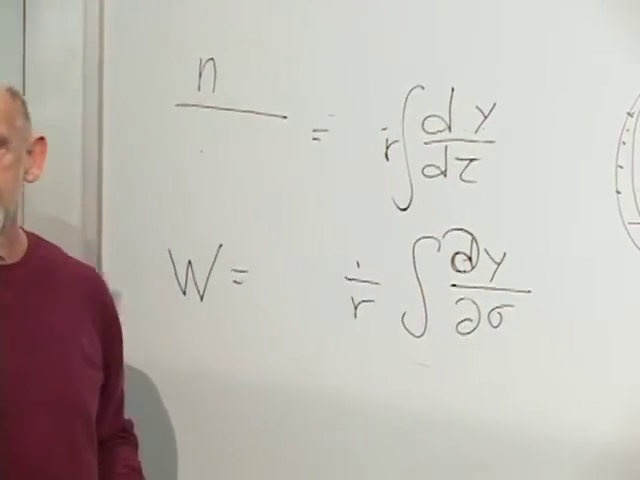
\includegraphics[width=0.72\textwidth]{lecture_10_figure_03.png}
  \medskip

  \begin{tikzpicture}[x=1cm,y=1cm,>=Latex]
    \draw[thick] (-4.0,0.3) circle (0.65);
    \draw[->,thick] (-4.55,0.58) arc (150:-145:0.65);
    \node at (-4.0,-0.65) {$w=+1$};
    \draw[thick] (-2.0,0.3) circle (0.65);
    \draw[->,thick] (-2.55,0.58) arc (150:-145:0.65);
    \node at (-2.0,-0.65) {$w=+1$};
    \node at (-3.0,0.3) {$+$};
    \draw[->,thick] (-1.0,0.3) -- (0.3,0.3);
    \draw[thick] (1.45,0.3) circle (0.78);
    \draw[thick] (1.45,0.3) circle (0.52);
    \draw[->,thick] (0.81,0.74) arc (145:-145:0.78);
    \node at (1.45,-0.78) {$w=+2$};
  \end{tikzpicture}
  \caption{Des enroulements de même signe peuvent se reconnecter en une corde doublement enroulée. La connectivité change, tandis que l’enroulement total reste égal à deux.}
  \lectureframe{00:16:40}
  \label{fig:l10-same-winding}
\end{figure}

Cette distinction subsiste dans tous les processus autorisés. Un enroulement total de cent peut être porté par une corde enroulée cent fois, deux cordes enroulées cinquante fois chacune, ou cent cordes enroulées une fois. Les cordes peuvent se scinder et fusionner entre ces configurations, mais la somme signée reste égale à cent. Nous la notons \(w\in\mathbb Z\).

\section{Modes d’impulsion et modes d’enroulement}

La conservation, à elle seule, ne suffit pas encore à établir la dualité. Comparons maintenant les énergies. L’impulsion d’un état se déplaçant autour du cercle compact est quantifiée :
\begin{equation}
  p_Y=\frac{n}{R},
  \qquad n\in\mathbb Z.
  \label{eq:l10-compact-momentum}
\end{equation}
Pour un état dont les autres contributions à la masse peuvent être négligées, le mouvement dans la direction compacte contribue à l’énergie sous la forme \(E_{\rm mom}=|n|/R\). Les valeurs positives et négatives de \(n\) correspondent à des sens de déplacement opposés, tandis que l’énergie reste positive.

\begin{figure}[H]
  \centering
  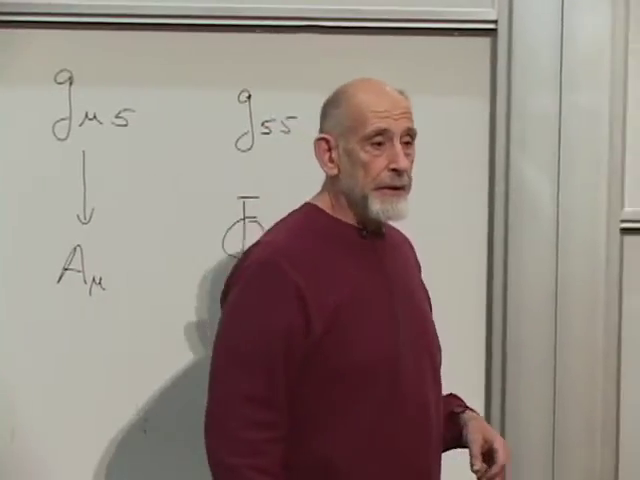
\includegraphics[width=0.72\textwidth]{lecture_10_figure_04.png}
  \caption{Le nombre quantique d’impulsion dans la direction compacte, tel qu’indiqué au tableau. Le cours représente schématiquement l’impulsion comme une intégrale de la vitesse dans cette direction.}
  \lectureframe{00:21:30}
  \label{fig:l10-compact-momentum-board}
\end{figure}

Une corde enroulée \(|w|\) fois a une longueur \(2\pi |w|R\). Avec une tension fondamentale de corde
\begin{equation}
  T_{\rm F}=\frac{1}{2\pi\alpha'},
\end{equation}
son énergie d’enroulement est
\begin{equation}
  E_{\rm wind}=T_{\rm F}(2\pi |w|R)
  =\frac{|w|R}{\alpha'}.
  \label{eq:l10-winding-energy}
\end{equation}
Dans les unités du cours, où \(\alpha'=1\), elle vaut simplement \(E_{\rm wind}=|w|R\).

Les deux tours de niveaux évoluent en sens opposés lorsque le rayon change. Pour \(R\gg
\sqrt{\alpha'}\), les niveaux d’impulsion sont rapprochés et ceux d’enroulement sont très espacés. Pour \(R\ll\sqrt{\alpha'}\), les niveaux d’impulsion sont très espacés et ceux d’enroulement sont rapprochés.

\begin{figure}[H]
  \centering
  \begin{minipage}[t]{0.48\textwidth}
    \centering
    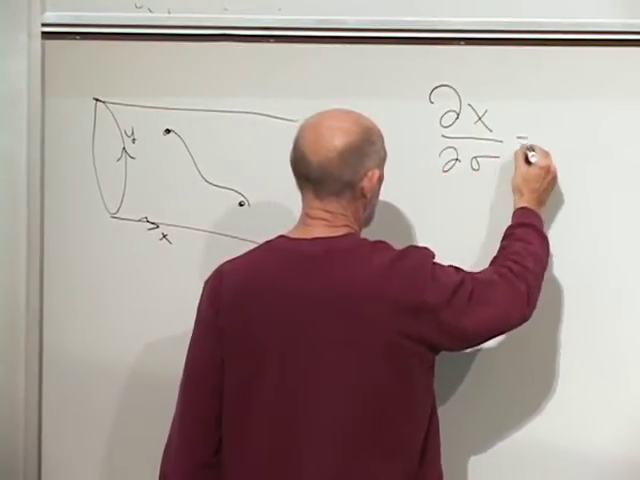
\includegraphics[width=\linewidth]{lecture_10_figure_05.png}
    \par\smallskip
    \textit{Grand rayon compact.}
  \end{minipage}\hfill
  \begin{minipage}[t]{0.48\textwidth}
    \centering
    \includegraphics[width=\linewidth]{lecture_10_figure_06.png}
    \par\smallskip
    \textit{Petit rayon compact.}
  \end{minipage}
  \caption{Les deux comparaisons spectrales présentées au tableau. Les tours clairsemés et denses échangent leurs rôles lorsque le rayon est inversé.}
  \lectureframe{00:25:30--00:26:00}
  \label{fig:l10-dual-spectra-board}
\end{figure}

Le schéma le plus simple est
\begin{figure}[H]
  \centering
  \begin{adjustbox}{max width=\linewidth}
  \begin{tikzpicture}[x=1cm,y=0.74cm,>=Latex]
    \node[font=\bfseries] at (-3.6,6.2) {$R\gg\sqrt{\alpha'}$};
    \draw[->] (-5.1,0) -- (-5.1,5.5) node[above] {$E$};
    \foreach \y in {0.4,1.0,1.6,2.2,2.8,3.4,4.0,4.6}
      \draw (-5.35,\y)--(-4.85,\y);
    \node[align=center] at (-4.25,5.15) {momentum\\dense};
    \draw[->] (-2.2,0) -- (-2.2,5.5) node[above] {$E$};
    \foreach \y in {0.4,2.4,4.4}
      \draw (-2.45,\y)--(-1.95,\y);
    \node[align=center] at (-1.35,5.15) {winding\\sparse};

    \node[font=\bfseries] at (3.6,6.2) {$R\ll\sqrt{\alpha'}$};
    \draw[->] (2.2,0) -- (2.2,5.5) node[above] {$E$};
    \foreach \y in {0.4,2.4,4.4}
      \draw (1.95,\y)--(2.45,\y);
    \node[align=center] at (3.05,5.15) {momentum\\sparse};
    \draw[->] (5.1,0) -- (5.1,5.5) node[above] {$E$};
    \foreach \y in {0.4,1.0,1.6,2.2,2.8,3.4,4.0,4.6}
      \draw (4.85,\y)--(5.35,\y);
    \node[align=center] at (5.95,5.15) {winding\\dense};
  \end{tikzpicture}
  \end{adjustbox}
  \caption{Reconstitution de l’argument fondé sur l’espacement des niveaux. Le spectre complet de la corde reste inchangé lorsque l’impulsion et l’enroulement sont échangés en même temps que \(R\leftrightarrow\alpha'/R\).}
  \label{fig:l10-dual-spectra-redraw}
\end{figure}

Supposons qu’on présente à un observateur l’un de ces spectres sans lui indiquer comment il a été obtenu. La tour de niveaux rapprochés correspond-elle à l’impulsion sur un grand cercle ou à l’enroulement sur un petit cercle ? Le spectre, à lui seul, ne permet pas de le dire. La théorie des cordes affirme plus fortement que les amplitudes de diffusion ne le permettent pas non plus. Les deux descriptions sont exactement équivalentes sous la transformation
\begin{equation}
  n\longleftrightarrow w,
  \qquad
  R\longleftrightarrow \widetilde R=\frac{\alpha'}{R}.
  \label{eq:l10-radius-duality}
\end{equation}
Le point fixe est
\begin{equation}
  R=\sqrt{\alpha'},
  \label{eq:l10-self-dual-radius}
\end{equation}soit \(R=1\) dans les unités du cours. À ce rayon, des états supplémentaires peuvent devenir sans masse et la symétrie de jauge est élargie.

\begin{classroomqa}
\audiencequestion{L’enroulement n’est-il qu’un artifice mathématique pour réécrire le spectre ? \lecturetimestamp{00:27:33}}
\lecturerresponse{Non. L’enroulement étiquette de véritables secteurs de l’espace de Hilbert de la corde fermée, et ces secteurs participent aux interactions. Le mot ``dualité'' signifie que les descriptions en termes d’impulsion et d’enroulement sont des coordonnées différentes d’une même physique, et non qu’un secteur n’est qu’un aide-mémoire facultatif pour l’autre.}
\end{classroomqa}

\begin{classroomqa}
\audiencequestion{Existe-t-il un rayon qui est envoyé sur lui-même ?
\lecturetimestamp{00:27:58}}
\lecturerresponse{Oui. La valeur auto-duale est
\(R=\sqrt{\alpha'}\), soit \(R=1\) dans les unités utilisées au tableau. Les deux tours se rejoignent en ce point, et le spectre présente une symétrie renforcée.}
\end{classroomqa}

\section{La forme de la dualité sur la feuille d’univers}

L’argument spectral est suggestif, mais la feuille d’univers rend l’échange plus précis. En jauge conforme, la quantité conjuguée à \(Y\) est proportionnelle à \(\partial_\tau Y\). L’impulsion compacte totale prend donc la forme
\begin{equation}
  P_Y=\frac{1}{2\pi\alpha'}
      \int_0^{2\pi}d\sigma\,\partial_\tau Y.
  \label{eq:l10-worldsheet-momentum}
\end{equation}
Le nombre d’enroulement vaut
\begin{equation}
  w=\frac{1}{2\pi R}
      \int_0^{2\pi}d\sigma\,\partial_\sigma Y
   =\frac{Y(2\pi)-Y(0)}{2\pi R}.
  \label{eq:l10-worldsheet-winding}
\end{equation}

\begin{classroomqa}
\audiencequestion{Pourquoi l’intégrale d’une dérivée ne s’annule-t-elle pas autour de la corde fermée ? \lecturetimestamp{00:32:33}}
\lecturerresponse{Parce que \(Y\) est une coordonnée périodique de l’espace cible, et non une fonction réelle univoque sur le cercle paramétré par \(\sigma\). Le point de la feuille d’univers \(\sigma=2\pi\) est identique à \(\sigma=0\), mais un relèvement de l’application d’immersion sur la droite de recouvrement varie de \(2\pi wR\). L’intégrale de \(\partial_\sigma Y\) mesure ce décalage.}
\end{classroomqa}

\begin{figure}[H]
  \centering
  \includegraphics[width=0.76\textwidth]{lecture_10_figure_07.png}
  \caption{Les intégrales de l’impulsion et de l’enroulement, une fois les deux lignes achevées au tableau. Les facteurs communs \(2\pi\) et \(\alpha'\) sont omis dans la normalisation du cours.}
  \lectureframe{00:33:25}
  \label{fig:l10-momentum-winding-integrals}
\end{figure}

Pour une corde enroulée une fois,
\begin{equation}
  Y(\tau,\sigma+2\pi)=Y(\tau,\sigma)+2\pi R.
\end{equation}
Pour un enroulement \(w\), le décalage du membre de droite vaut \(2\pi wR\). L’équation \eqref{eq:l10-worldsheet-winding} compte alors exactement l’enroulement. C’est la formulation précise de l’abréviation utilisée au tableau : \(w\sim R^{-1}\int
d\sigma\,\partial_\sigma Y\).

La formulation de la T-dualité sur la feuille d’univers est donc
\begin{equation}
  \partial_\tau Y\longleftrightarrow
  \partial_\sigma \widetilde Y,
  \qquad
  \partial_\sigma Y\longleftrightarrow
  \partial_\tau \widetilde Y,
  \label{eq:l10-derivative-duality}
\end{equation}
l’impulsion dans \(Y\) devenant l’enroulement dans la coordonnée duale \(\widetilde Y\), et réciproquement.

\begin{classroomqa}
\audiencequestion{Cela signifie-t-il que les coordonnées de la feuille d’univers \(\tau\) et \(\sigma\) sont elles-mêmes reliées ou échangées ?
\lecturetimestamp{00:34:39}}
\lecturerresponse{Non. La T-dualité associe des solutions et échange certaines dérivées de la coordonnée compacte de l’espace cible. Elle n’identifie pas la coordonnée temporelle de la feuille d’univers à sa coordonnée spatiale.}
\end{classroomqa}

\section{Pourquoi les états enroulés sont inévitables}

On peut se demander pourquoi une corde se trouverait dans un état enroulé alors qu’un état non enroulé est possible. Une corde ne choisit pas son état par préférence. L’énergie fournie lors d’une collision l’étire. Une corde suffisamment énergétique et fortement déformée peut se reconnecter en deux cordes d’enroulements opposés. Leur enroulement total reste nul, mais les deux cordes peuvent s’éloigner l’une de l’autre après la scission. L’une d’elles peut être envoyée très loin, laissant un observateur face à une corde enroulée apparemment isolée.

\begin{figure}[H]
  \centering
  \includegraphics[width=0.76\textwidth]{lecture_10_figure_08.png}
  \caption{Une configuration fortement étirée d’enroulement total nul, à partir de laquelle des cordes d’enroulements opposés peuvent s’éloigner après reconnexion.}
  \lectureframe{00:36:15}
  \label{fig:l10-winding-pair-production}
\end{figure}

Le seuil d’énergie est fixé par l’énergie d’enroulement. Sur un grand cercle, il faut une énergie de collision élevée pour étirer suffisamment la corde afin qu’elle fasse le tour de la direction compacte. Au-delà du seuil, cependant, la production de paires corde enroulée--anti-corde enroulée ne peut être interdite. L’analogie est celle de collisions de photons produisant une paire électron--positon. La charge électrique totale reste nulle, mais les particules chargées sont bien présentes et peuvent être séparées. La conservation de l’enroulement fonctionne de la même manière.

Cette analogie ne se limite pas aux mots. L’impulsion compacte et l’enroulement se comportent comme deux nombres quantiques de charge distincts. Dans la description réduite correspondante, les charges de même signe se repoussent et celles de signes opposés s’attirent. Il faut donc chercher les deux champs vectoriels qui transmettent ces forces.

\section{Charge d’impulsion issue de la gravitation en cinq dimensions}

Commençons par la gravitation en cinq dimensions. Les indices majuscules \(M,N\) parcourent les quatre directions ordinaires de l’espace-temps et la cinquième direction compacte. La métrique se décompose comme suit :
\begin{equation}
  G_{MN}\quad\longrightarrow\quad
  \bigl\{G_{\mu\nu},\,G_{\mu5},\,G_{55}\bigr\}.
  \label{eq:l10-metric-decomposition}
\end{equation}
La composante symétrique \(G_{5\mu}\) n’apporte aucune information nouvelle par rapport à \(G_{\mu5}\).

\begin{figure}[H]
  \centering
  \includegraphics[width=0.74\textwidth]{lecture_10_figure_09.png}
  \caption{Les groupes indépendants de composantes de la métrique en cinq dimensions : \(G_{\mu\nu}\), \(G_{\mu5}\) et \(G_{55}\).}
  \lectureframe{00:44:05}
  \label{fig:l10-metric-components}
\end{figure}

Du point de vue quadridimensionnel,
\begin{align}
  G_{\mu\nu} &\quad\hbox{is a spacetime metric},\\
  G_{\mu5} &\equiv A_\mu\quad\hbox{is a vector field},\\
  G_{55} &\equiv e^{2\varphi}\quad\hbox{is a scalar modulus}.
  \label{eq:l10-four-dimensional-fields}
\end{align}
Le scalaire \(\varphi\) mesure la taille de la direction compacte. Il peut varier de façon continue dans l’espace-temps ordinaire ; les ondes de \(\varphi\) sont donc des variations du rayon de la cinquième dimension.

\begin{figure}[H]
  \centering
  \includegraphics[width=0.74\textwidth]{lecture_10_figure_10.png}
  \caption{Au tableau, \(G_{\mu5}\) est identifié à un vecteur \(A_\mu\) et \(G_{55}\) à un scalaire \(\Phi\).}
  \lectureframe{00:47:40}
  \label{fig:l10-vector-and-radius-modulus}
\end{figure}

Une composante gravitationnelle mixte a pour source un flux d’impulsion mixte. En particulier, l’impulsion dans la cinquième direction source \(G_{\mu5}\). Un observateur quadridimensionnel interprète donc l’entier \(n\) comme une charge électrique couplée à \(A_\mu\). C’est le mécanisme de Kaluza--Klein : une quantité qui est une impulsion dans la géométrie de dimension supérieure devient une charge dans la théorie des champs de dimension inférieure.

\editorialnote{Dans le cours, le scalaire issu de \(G_{55}\) est appelé de façon approximative « ``dilaton'' ». Dans cette réduction, il s’agit précisément du module du rayon. Le dilaton de la corde en dix dimensions, qui détermine le couplage de la corde, est un champ distinct, même si des combinaisons scalaires de dimension inférieure peuvent se mélanger lors de changements de cadre et de dualité.}

\begin{classroomqa}
\audiencequestion{Le scalaire \(\varphi\) est-il proportionnel à l’entier d’impulsion \(n\) ? \lecturetimestamp{00:48:43}}
\lecturerresponse{Non. L’entier \(n\) étiquette un état quantifié et joue le rôle d’une charge. Le scalaire \(\varphi(x)\) est un champ continu qui détermine la taille locale de la compactification. Il peut varier d’un endroit à l’autre ; il n’est pas lui-même un entier.}
\end{classroomqa}

\section{Le second champ vectoriel et la charge d’enroulement}

L’enroulement se comporte lui aussi comme une charge, mais il ne peut pas se coupler de la même manière au même vecteur. Pour faire apparaître le second vecteur, revenons aux premières excitations de la corde fermée. Une corde fermée possède des modes oscillatoires gauches et droits. Les états physiques satisfont la condition d’appariement des niveaux : les niveaux totaux d’excitation gauche et droit doivent être égaux.

Dans la théorie bosonique, l’état non excité est le tachyon. Un oscillateur unique, gauche ou droit, ne satisferait pas l’appariement des niveaux. Le premier état sans masse autorisé contient donc un oscillateur de chaque type :
\begin{equation}
  \alpha_{-1}^{I}\widetilde\alpha_{-1}^{J}\ket{0;k}.
  \label{eq:l10-first-massless-state}
\end{equation}
Les indices \(I,J\) parcourent les directions spatiales transverses, y compris la direction compacte. Si l’un des indices correspond à une direction ordinaire et l’autre à \(5\), on obtient deux états d’oscillateur de type vectoriel :
\begin{equation}
  \alpha_{-1}^{\mu}\widetilde\alpha_{-1}^{5}\ket{0;k},
  \qquad
  \alpha_{-1}^{5}\widetilde\alpha_{-1}^{\mu}\ket{0;k}.
  \label{eq:l10-two-vector-states}
\end{equation}

\begin{figure}[H]
  \centering
  \includegraphics[width=0.76\textwidth]{lecture_10_figure_11.png}
  \caption{Les deux ordres d’oscillateurs gauche--droit qui deviennent des états vectoriels quadridimensionnels lorsqu’une polarisation pointe dans la direction compacte.}
  \lectureframe{00:58:20}
  \label{fig:l10-two-vector-states-board}
\end{figure}

Leurs combinaisons symétrique et antisymétrique appartiennent à des champs distincts de l’espace-temps :
\begin{align}
  \alpha_{-1}^{(\mu}\widetilde\alpha_{-1}^{5)}\ket{0;k}
    &\longleftrightarrow G_{\mu5},\\
  \alpha_{-1}^{[\mu}\widetilde\alpha_{-1}^{5]}\ket{0;k}
    &\longleftrightarrow B_{\mu5}.
  \label{eq:l10-g-and-b-vectors}
\end{align}
Le premier est le vecteur de Kaluza--Klein, dont la source est l’impulsion compacte. Le second provient du champ antisymétrique de Kalb--Ramond et a pour source l’enroulement de la corde. La théorie réduite contient donc deux champs analogues au photon, un pour chaque secteur de charge.

Si les deux indices de l’oscillateur pointent dans la direction compacte, l’état est un scalaire associé au module de compactification. S’ils pointent tous deux dans des directions transverses ordinaires, la partie symétrique sans trace est le graviton, la partie antisymétrique est \(B_{\mu\nu}\) et la trace contribue à un secteur scalaire.

\begin{classroomqa}
\audiencequestion{Lequel de ces états est le singulet et lequel est le triplet ? \lecturetimestamp{01:00:21}}
\lecturerresponse{Cette classification n’est pas pertinente ici. Les deux états mixtes se transforment comme des vecteurs quadridimensionnels. Leur somme et leur différence séparent la polarisation symétrique de la métrique de la polarisation antisymétrique du champ \(B\). L’état dont les deux indices sont compacts est, lui, un scalaire quadridimensionnel.}
\end{classroomqa}

Le dictionnaire complet établi avant la pause est le suivant :
\begin{equation}
  \boxed{
  \begin{gathered}
    n\leftrightarrow w,
    \qquad
    R\leftrightarrow\dfrac{\alpha'}{R},\\
    \partial_\tau Y\leftrightarrow\partial_\sigma\widetilde Y,
    \qquad
    G_{\mu5}\leftrightarrow B_{\mu5}.
  \end{gathered}}
  \label{eq:l10-complete-t-duality-map}
\end{equation}

\begin{figure}[H]
  \centering
  \includegraphics[width=0.72\textwidth]{lecture_10_figure_12.png}
  \caption{Récapitulatif au tableau de la transformation de T-dualité : l’impulsion et l’enroulement, le rayon et son inverse, les dérivées de la feuille d’univers et les deux champs vectoriels sont échangés. Le conférencier masque en partie la dernière ligne ; elle est donc donnée explicitement dans l’équation \eqref{eq:l10-complete-t-duality-map}.}
  \lectureframe{01:02:20}
  \label{fig:l10-t-duality-map-board}
\end{figure}

Cette construction ne doit pas être confondue avec l’affirmation que tous les champs énumérés ont déjà été identifiés dans le spectre observé des particules. À ce stade, il s’agit d’une conséquence mathématique de la théorie des cordes compactifiée. Il existe de nombreuses propositions pour relier de telles structures à la phénoménologie, mais ce n’est pas le problème traité dans ce cours.

\section{Les cordes ouvertes changent la question}

Après la pause, nous reprenons avec les cordes ouvertes. Une corde fermée peut avoir un enroulement stable, car elle n’a pas d’extrémité par laquelle celui-ci pourrait s’échapper. Une corde ouverte a des extrémités et ne possède donc pas d’enroulement analogue protégé topologiquement. Pourtant, la T-dualité est une symétrie exacte de la théorie. Que fait cette symétrie à une corde ouverte ?

Pour une extrémité libre de se déplacer, la variation de l’action de la corde donne une condition aux limites de Neumann. Dans la géométrie simple \((X,Y)\),
\begin{equation}
  \left.\partial_\sigma X\right|_{\partial\Sigma}=0,
  \qquad
  \left.\partial_\sigma Y\right|_{\partial\Sigma}=0.
  \label{eq:l10-neumann-boundary}
\end{equation}
L’interprétation mécanique est directe. Considérons la corde comme une chaîne composée d’éléments de masse de plus en plus petits. Une force tangentielle non nulle sur le dernier élément lui imprimerait une accélération qui diverge lorsque sa masse tend vers zéro. Une extrémité libre se déplace donc jusqu’à ce que la tension résultante à l’extrémité s’annule. On pourrait aussi maintenir l’extrémité fixe et fournir la force nécessaire, mais elle ne serait alors plus libre.

\begin{figure}[H]
  \centering
  \includegraphics[width=0.76\textwidth]{lecture_10_figure_13.png}
  \caption{La corde ouverte et ses conditions de Neumann aux extrémités, une fois complétées : \(\partial_\sigma X=\partial_\sigma Y=0\).}
  \lectureframe{01:09:20}
  \label{fig:l10-neumann-board}
\end{figure}

Effectuons maintenant la dualité uniquement sur la coordonnée compacte \(Y\). La coordonnée non compacte \(X\) reste inchangée. L’équation \eqref{eq:l10-derivative-duality} transforme la seconde condition de Neumann en
\begin{equation}
  \left.\partial_\tau\widetilde Y\right|_{\partial\Sigma}=0.
  \label{eq:l10-dirichlet-time-derivative}
\end{equation}
L’extrémité a donc une position indépendante du temps dans la direction compacte duale :
\begin{equation}
  \left.\widetilde Y\right|_{\partial\Sigma}=Y_0.
  \label{eq:l10-dirichlet-boundary}
\end{equation}
C’est une condition aux limites de Dirichlet.

\begin{figure}[H]
  \centering
  \includegraphics[width=0.76\textwidth]{lecture_10_figure_14.png}
  \medskip

  \begin{adjustbox}{max width=\linewidth}
  \begin{tikzpicture}[x=1cm,y=1cm,>=Latex]
    \node[align=center] at (-3.5,0.8)
      {Neumann\\\(\left.\partial_\sigma Y\right|_{\partial\Sigma}=0\)};
    \draw[->,thick] (-1.7,0.8) -- (1.3,0.8)
      node[midway,above] {$T_Y$};
    \node[align=center] at (3.4,0.8)
      {Dirichlet\\\(\left.\partial_\tau\widetilde Y\right|_{\partial\Sigma}=0\)};
    \node[align=center] at (3.4,-0.5)
      {\(\widetilde Y(\tau)=Y_0\) at each endpoint};
  \end{tikzpicture}
  \end{adjustbox}
  \caption{La condition complète imposée à l’extrémité duale, telle qu’écrite au tableau, et sa reconstruction logique. La T-dualité transforme la liberté de mouvement dans la direction compacte en une position fixe de l’extrémité dans la direction duale.}
  \lectureframe{01:12:35}
  \label{fig:l10-neumann-to-dirichlet}
\end{figure}

\begin{classroomqa}
\audiencequestion{Pourquoi la condition duale signifie-t-elle que l’extrémité est fixe ? \lecturetimestamp{01:12:39}}
\lecturerresponse{Parce que \(\partial_\tau\widetilde Y=0\) signifie que la vitesse dans la direction dualisée est nulle. Quelle que soit la position initiale de l’extrémité en \(\widetilde Y\), elle y reste. Ses coordonnées dans les directions parallèles non dualisées restent libres.}
\end{classroomqa}

\section{L’objet qui retient l’extrémité est une D-brane}

Si une extrémité est fixe, quelque chose doit pouvoir la maintenir en place. La T-dualité exacte exige donc un nouvel objet auquel les cordes ouvertes peuvent se terminer : une D-brane. La lettre \(D\) désigne Dirichlet, et non la dimension de l’objet. Dans l’anecdote historique racontée pendant le cours, ces objets auraient pu être nommés d’après Joseph Polchinski, dont l’analyse a rendu leur rôle dynamique indiscutable ; cependant, le terme déjà établi ``p-brane'' faisait de Dirichlet un nom naturel.

Une \(p\)-brane possède \(p\) dimensions spatiales. Une corde est une 1-brane, une membrane une 2-brane, et un objet étendu à trois dimensions une 3-brane. Une D\(p\)-brane est une \(p\)-brane sur laquelle les extrémités des cordes fondamentales satisfont des conditions de Dirichlet dans les directions transverses à la brane et des conditions de Neumann dans les directions qui lui sont tangentes.

Rien dans l’argument de dualité ne privilégie une valeur particulière de \(Y_0\) ; la D-brane ne peut donc pas être un élément rigide cloué en un point privilégié de l’univers. Elle doit pouvoir se déplacer. La relativité interdit aussi l’existence d’un corps étendu absolument rigide ; une D-brane peut donc fluctuer et se courber. La brane plane dessinée au tableau représente sa configuration d’équilibre, et non une restriction de sa dynamique.

\begin{classroomqa}
\audiencequestion{Les deux extrémités d’une corde ouverte doivent-elles avoir la même valeur fixe de la coordonnée duale ? \lecturetimestamp{01:14:55}}
\lecturerresponse{Pas en général. Les deux extrémités peuvent se trouver sur la même D-brane ; elles partagent alors la position transverse de celle-ci. Elles peuvent aussi se trouver sur deux D-branes différentes, situées à des positions transverses distinctes, auquel cas la corde s’étire entre elles. Une brane peut elle-même fluctuer et se courber ; le lieu des extrémités ne reste donc pas nécessairement un plan parfaitement plat.}
\end{classroomqa}

\section{Compter les dimensions d’une D-brane}

La théorie des supercordes en dix dimensions possède neuf dimensions spatiales. Supposons que la T-dualité impose une condition de Dirichlet dans une direction spatiale. L’extrémité reste libre dans les huit autres directions ; son lieu possible est donc une D8-brane de dimension huit. Chaque condition de Dirichlet indépendante supplémentaire supprime une direction de mouvement de l’extrémité. Si \(k\) coordonnées spatiales sont fixées, alors
\begin{equation}
  p=9-k.
  \label{eq:l10-dp-counting}
\end{equation}

La table illustre le même décompte en trois dimensions. Si l’on fixe la coordonnée verticale, le bout du doigt peut se déplacer sur une table bidimensionnelle. Si l’on fixe une deuxième coordonnée, il ne peut plus se déplacer que le long d’une ligne. Si l’on fixe les trois, il est confiné en un point.

\begin{figure}[H]
  \centering
  \begin{adjustbox}{max width=\linewidth}
  \begin{tikzpicture}[x=1.05cm,y=1cm,>=Latex]
    \draw[fill=blue!8] (-5.5,-0.7) -- (-2.5,-0.7) -- (-1.7,0.2)
      -- (-4.7,0.2) -- cycle;
    \node at (-3.6,-1.15) {one constraint: sheet};
    \draw[very thick,blue!60!black] (-0.9,-0.25) -- (1.3,-0.25);
    \node at (0.2,-1.15) {two constraints: line};
    \fill[blue!70!black] (4.1,-0.25) circle (0.09);
    \node at (4.1,-1.15) {three constraints: point};
    \draw[->] (-1.45,0.95) -- (-0.75,0.95);
    \draw[->] (2.25,0.95) -- (2.95,0.95);
    \node at (0.35,1.35) {each Dirichlet condition lowers \(p\) by one};
  \end{tikzpicture}
  \end{adjustbox}
  \caption{L’argument de décompte des dimensions illustré sur la table. Une D\(p\)-brane est le lieu où les extrémités restent libres de se déplacer.}
  \label{fig:l10-dp-counting-redraw}
\end{figure}

Des dualités répétées produisent des D8-, D7- et D6-branes, et ainsi de suite jusqu’à une D0-brane, ponctuelle dans l’espace. Si aucune direction spatiale n’est fixée, une D9-brane remplit les neuf dimensions spatiales et les cordes ouvertes ordinaires peuvent se déplacer partout. Le cours mentionne brièvement les D-branes D\((-1)\) : elles sont localisées dans l’espace-temps euclidien et se comportent comme des instantons plutôt que comme des particules ordinaires se propageant dans le temps.

\editorialnote{L’échelle des dimensions concerne les théories de type II considérées ensemble. Pour les D\(p\)-branes BPS stables, \(p\) est pair en type IIA et \(p\) impair en type IIB. La T-dualité le long d’un cercle modifie \(p\) d’une unité et échange simultanément les théories de type IIA et de type IIB.}

\begin{classroomqa}
\audiencequestion{Si seules six dimensions sont compactes, faut-il commencer le décompte en soustrayant de six plutôt que de neuf ? \lecturetimestamp{01:20:49}}
\lecturerresponse{La démonstration élémentaire applique la T-dualité aux directions compactes, mais le cercle dual devient arbitrairement grand lorsque le cercle initial devient arbitrairement petit. Dans cette limite, il est effectivement non compact. Les branes obtenues peuvent donc s’étendre dans des directions qui paraissent non compactes aux échelles accessibles, ou leur être transverses. La dimension \(p\) compte toutes les directions spatiales tangentes à la brane, et pas seulement les directions compactes utilisées dans une démonstration donnée.}
\end{classroomqa}

Une D0-brane est un nouveau type de particule. Une corde ouverte peut partir d’une D0-brane et se terminer sur une autre, revenir sur la même D0-brane ou s’étirer vers une brane très éloignée. Une corde allant littéralement jusqu’à l’infini spatial aurait une longueur et donc une énergie infinies ; dans la configuration physiquement utile, son autre extrémité se trouve sur un autre objet.

Le cas suivant, une D1-brane, a lui aussi la forme d’une corde, mais ce n’est pas la corde fondamentale par laquelle nous avons commencé. Elle peut se courber et se refermer sur elle-même, et des cordes fondamentales peuvent y prendre fin. Sa tension dépend du couplage des cordes d’une autre manière :
\begin{equation}
  T_{\rm D1}=\frac{1}{2\pi\alpha' g_s},
  \qquad
  T_{\rm F1}=\frac{1}{2\pi\alpha'}.
  \label{eq:l10-dstring-tension}
\end{equation}
À faible couplage \(g_s\ll1\), la corde D est beaucoup plus lourde que la corde fondamentale, ce qui explique qu’elle apparaisse d’abord comme un ancrage massif.

\begin{figure}[H]
  \centering
  \includegraphics[width=0.76\textwidth]{lecture_10_figure_15.png}
  \caption{La D1-brane du tableau : un objet unidimensionnel déformable, distinct des cordes fondamentales qui peuvent y prendre fin.}
  \lectureframe{01:24:20}
  \label{fig:l10-d1-brane}
\end{figure}

\begin{classroomqa}
\audiencequestion{La dualité T agit-elle sur les D-branes aussi bien que sur les cordes ? \lecturetimestamp{01:25:35}}
\lecturerresponse{Oui. Une dualité T parallèle à une D\(p\)-brane abaisse sa dimension à D\((p-1)\), tandis qu’une dualité T transverse à celle-ci l’élève à D\((p+1)\). Les branes font partie du dictionnaire de dualité ; elles ne sont pas des supports extérieurs que celle-ci laisserait inchangés.}
\end{classroomqa}

\begin{classroomqa}
\audiencequestion{Des directions tangentes à une brane peuvent-elles malgré tout être compactes ?
\lecturetimestamp{01:27:25}}
\lecturerresponse{Oui. ``Tangente'' et ``compacte'' répondent à des questions différentes. Une direction peut être parallèle à la brane tout en se refermant sur un cercle ; elle peut aussi être non compacte. Pour l’extrémité de la corde, ce qui importe, c’est que la condition aux limites dans cette direction soit de Neumann ou de Dirichlet.}
\end{classroomqa}

Une D2-brane est une membrane en forme de feuille. Une D3-brane a trois dimensions spatiales. Dans un espace-temps véritablement de dimension supérieure, une D3-brane est un sous-espace tridimensionnel et non la totalité de l’espace, même si les observateurs qui y sont confinés peuvent la percevoir comme l’ensemble de leur espace spatial.

\begin{figure}[H]
  \centering
  \includegraphics[width=0.76\textwidth]{lecture_10_figure_16.png}
  \caption{Une D2-brane représentée comme une feuille sur laquelle les extrémités des cordes peuvent se déplacer.}
  \lectureframe{01:27:55}
  \label{fig:l10-d2-brane}
\end{figure}

La dérivation présentée ici est volontairement schématique. À elle seule, elle ne prouve pas que la théorie des cordes décrit la nature. Au sein de la théorie des cordes, toutefois, les vérifications de cohérence sont nombreuses : les dualités, les calculs quantiques et les résultats mathématiques indiquent tous que les D-branes sont de véritables objets dynamiques.

\section{Les cordes ouvertes deviennent des champs sur une brane}

Considérons une D2-brane par ailleurs vide et plaçons-y de courtes cordes ouvertes. Chaque extrémité est confinée à la feuille, de sorte que toute excitation de basse énergie se déplace le long de celle-ci. Deux cordes orientées dont les extrémités adjacentes portent des flèches compatibles peuvent s’assembler. La corde ainsi formée peut ensuite se séparer de nouveau. Interprétés comme des trajectoires de particules, ces processus correspondent aux sommets des diagrammes de Feynman : deux particules entrent, une excitation intermédiaire se propage, puis deux particules ressortent.

\begin{figure}[H]
  \centering
  \includegraphics[width=0.76\textwidth]{lecture_10_figure_17.png}
  \caption{Des cordes ouvertes orientées sur une D2-brane s’assemblent lorsque leurs extrémités sont compatibles. À basse énergie, ce processus s’interprète comme une interaction de théorie des champs sur la brane.}
  \lectureframe{01:29:55}
  \label{fig:l10-open-strings-on-brane}
\end{figure}

À des énergies bien inférieures à l’échelle des cordes, la tour des modes vibrationnels internes n’est pas excitée. Il reste alors l’état sans masse de la corde ouverte, qui est un champ vectoriel sur le volume d’univers de la brane. Pour une seule brane, il s’agit d’un champ de jauge abélien \(U(1)\), l’analogue de l’électromagnétisme pour une brane. Le champ ne se propage pas dans tout le volume ambiant à dix dimensions ; ses quanta sont des cordes ouvertes dont les extrémités les maintiennent sur la brane.

\section{Un empilement de branes produit une couleur non abélienne}

Plaçons maintenant plusieurs branes parallèles à proximité les unes des autres. Pour trois branes, appelons-les Rouge, Vert et Bleu. Une corde orientée porte une paire ordonnée d’étiquettes à ses extrémités : elle peut aller de Rouge à Vert, de Vert à Bleu, de Rouge à Rouge, et ainsi de suite. Avec \(N\) branes, les états sans masse des cordes ouvertes peuvent être organisés en une matrice \(N\times N\)
\begin{equation}
  A_\mu{}^{i}{}_{j},
  \qquad i,j=1,\ldots,N.
  \label{eq:l10-chan-paton-matrix}
\end{equation}
Ce sont les étiquettes de Chan--Paton d’une théorie de jauge \(U(N)\).

\begin{figure}[H]
  \centering
  \includegraphics[width=0.76\textwidth]{lecture_10_figure_18.png}
  \medskip

  \begin{adjustbox}{max width=\linewidth}
  \begin{tikzpicture}[x=1cm,y=1cm,>=Latex]
    \draw[very thick,red!70!black] (-4.8,2.0)--(4.8,2.0);
    \draw[very thick,green!55!black] (-4.8,0.8)--(4.8,0.8);
    \draw[very thick,blue!70!black] (-4.8,-0.4)--(4.8,-0.4);
    \node[left] at (-4.8,2.0) {Red};
    \node[left] at (-4.8,0.8) {Green};
    \node[left] at (-4.8,-0.4) {Blue};
    \draw[->,thick] (-3.4,2.0) .. controls (-2.8,1.35) and (-2.3,1.15)
      .. (-1.7,0.8);
    \node at (-2.7,1.05) {$R\!G$};
    \draw[->,thick] (-0.6,0.8) .. controls (0.0,0.25) and (0.6,-0.05)
      .. (1.2,-0.4);
    \node at (0.1,0.0) {$G\!B$};
    \draw[->,thick] (2.1,2.0) .. controls (2.9,2.55) and (3.8,2.55)
      .. (4.3,2.0);
    \node at (3.2,2.65) {$R\!R$};
  \end{tikzpicture}
  \end{adjustbox}
  \caption{Trois branes parallèles au tableau et une reconstruction claire des étiquettes ordonnées des extrémités portées par les cordes qui les relient.}
  \lectureframe{01:33:15}
  \label{fig:l10-three-brane-stack}
\end{figure}

\begin{classroomqa}
\audiencequestion{Une corde peut-elle vraiment aller de la brane Rouge à la brane Verte sans être bloquée par les autres traits du dessin ? \lecturetimestamp{01:35:07}}
\lecturerresponse{Oui. Les branes sont plongées dans un espace de dimension supérieure. Le dessin sur un tableau à deux dimensions n’est qu’une projection ; une corde peut donc contourner un autre trait projeté en passant dans une direction transverse.}
\end{classroomqa}

\begin{classroomqa}
\audiencequestion{Une corde Rouge--Vert doit-elle s’assembler avec une corde Vert--Bleu pour devenir une corde Rouge--Bleu ? \lecturetimestamp{01:35:39}}
\lecturerresponse{C’est la règle fondamentale d’assemblage local. Des extrémités compatibles se rejoignent, et les deux segments forment une seule corde dont les extrémités libres conservent leurs étiquettes Rouge et Bleu. Les processus plus élaborés se construisent en répétant la même opération.}
\end{classroomqa}

La règle d’assemblage est la multiplication matricielle rendue géométrique. Une corde Rouge--Vert peut s’assembler avec une corde Vert--Bleu, car l’extrémité Verte de l’une est compatible avec l’extrémité Verte de l’autre. Le résultat est une corde Rouge--Bleu :
\begin{equation}
  (R,G)\circ(G,B)\longrightarrow(R,B).
  \label{eq:l10-color-composition}
\end{equation}
L’indice répété est raccordé et disparaît à l’intérieur. On retrouve cette même structure d’indices au sommet d’interaction de Yang--Mills.

\begin{figure}[H]
  \centering
  \includegraphics[width=0.76\textwidth]{lecture_10_figure_19.png}
  \caption{Assemblage de cordes ouvertes sur un empilement de branes. L’orientation des extrémités impose la même composition d’indices ordonnés que celle des champs de jauge non abéliens.}
  \lectureframe{01:36:30}
  \label{fig:l10-color-joining-board}
\end{figure}

Pour trois branes coïncidentes, le groupe de jauge complet des cordes ouvertes est \(U(3)\), avec neuf états vectoriels. Son algèbre se décompose ainsi :
\begin{equation}
  \mathfrak u(3)=\mathfrak{su}(3)\oplus\mathfrak u(1).
  \label{eq:l10-u3-decomposition}
\end{equation}
Les huit combinaisons sans trace ont la structure de couleur des gluons de la QCD, tandis que \(U(1)\), le centre de masse diagonal, est un champ abélien distinct.

\editorialnote{Le cours décrit l’une des neuf combinaisons de paires de couleurs comme pouvant se détacher et disparaître, ne laissant ainsi que huit gluons. La formulation précise pour les D-branes est qu’un empilement de trois branes coïncidentes donne \(U(3)\), et pas seulement \(SU(3)\). Pour obtenir l’octet de la QCD, il faut séparer, projeter ou découpler d’une autre manière le \(U(1)\) diagonal. L’image du cours illustre correctement les indices de couleur ordonnés, mais ne constitue pas une dérivation complète de la QCD.}

La matière de type quark porte un seul indice de couleur. Dans l’image des branes, elle est représentée par une corde dont une extrémité se trouve sur l’empilement de branes de couleur et l’autre sur une brane différente, éloignée. Par rapport à cet empilement, une seule extrémité porte une étiquette de couleur visible. L’inversion de l’orientation donne l’antiparticule. Une corde de type quark et une corde de type antiquark dont les extrémités sont compatibles peuvent s’assembler et quitter l’empilement de branes de couleur ; deux cordes de type quark ayant la même orientation ne peuvent pas s’annihiler de cette façon.

Les théories de basse énergie obtenues sont généralement des théories de Yang--Mills supersymétriques, avec de la matière supplémentaire déterminée par les branes et leurs intersections. Elles sont suffisamment proches de la QCD pour éclairer la dynamique non abélienne, mais elles ne sont pas automatiquement le Modèle standard. Avec une seule brane, la même construction se réduit à une théorie \(U(1)\) : les courtes cordes brane--brane sont analogues aux photons, tandis que les cordes orientées qui atteignent un second secteur jouent le rôle des charges électriques positives et négatives.

\section{Les cordes D prennent fin en monopoles magnétiques}

Il y a maintenant deux sortes d’objets de type corde dans cette histoire. La corde fondamentale, ou corde F, porte un flux électrique sur une D3-brane. La D1-brane, ou corde D, est beaucoup plus lourde à faible couplage. Une corde D peut elle aussi prendre fin sur une D3-brane. Son extrémité n’est pas chargée électriquement sous le champ de jauge du volume d’univers ; elle porte une charge magnétique. Pour les observateurs sur la D3-brane, cette extrémité est un monopole magnétique.

\begin{figure}[H]
  \centering
  \includegraphics[width=0.76\textwidth]{lecture_10_figure_20.png}
  \medskip

  \begin{adjustbox}{max width=\linewidth}
  \begin{tikzpicture}[x=1cm,y=1cm,>=Latex]
    \draw[fill=blue!7] (-3.8,-0.5)--(2.6,-0.5)--(3.6,0.35)--(-2.8,0.35)--cycle;
    \node at (2.25,-0.95) {D3-brane};
    \draw[very thick,red!70!black] (0.0,3.0)--(0.0,0.0);
    \fill[black] (0.0,0.0) circle (0.08);
    \node[right] at (0.15,2.1) {D-string};
    \foreach \a in {25,65,115,155} {
      \draw[->,blue!65!black] (0.0,0.0)--({1.25*cos(\a)},{0.65*sin(\a)});
    }
    \node[align=center] at (4.8,1.7) {magnetic flux\\on the D3 worldvolume};
    \draw[->] (3.7,1.35)--(1.05,0.45);
  \end{tikzpicture}
  \end{adjustbox}
  \caption{La construction du point d’extrémité au tableau et son interprétation précise. Une corde D qui prend fin sur une D3-brane apparaît comme un monopole magnétique pour la théorie de jauge du volume d’univers.}
  \lectureframe{01:41:30}
  \label{fig:l10-dstring-monopole}
\end{figure}

La hiérarchie des masses présente aussi la forme qualitative attendue. Puisque la tension de la corde D comporte un facteur \(1/g_s\), son extrémité est beaucoup plus lourde qu’une excitation électrique ordinaire à faible couplage. La relation électrique et magnétique entre les extrémités des cordes F et D fait partie de la structure plus vaste des dualités de la théorie des cordes de type IIB.

\begin{classroomqa}
\audiencequestion{L’extrémité de la corde D est-elle neutre ?
\lecturetimestamp{01:42:19}}
\lecturerresponse{Elle est neutre vis-à-vis de la charge électrique portée par une extrémité de corde fondamentale, mais elle n’est pas dépourvue de charge. Elle porte une charge magnétique et constitue donc un monopole dans la théorie de jauge de la D3-brane.}
\end{classroomqa}

\section{Ce que la construction affirme et ce qu’elle n’affirme pas}

Le chemin qui mène de la dualité T aux branes s’est construit au fil de plusieurs décennies, et non en un seul calcul. Une théorie d’abord proposée pour décrire les hadrons est devenue une théorie candidate de la gravité quantique. Ses dualités ont ensuite imposé la présence des D-branes dans le spectre, et les théories de jauge sont réapparues comme dynamique de basse énergie des cordes qui prennent fin sur ces branes. En ce sens, le sujet a bouclé la boucle.

Les D-branes et les constructions duales qui leur sont apparentées sont devenues de puissants outils pour étudier les théories de jauge supersymétriques, les systèmes fortement couplés et les liens entre gravité et théorie des champs. Elles ont également contribué à l’étude des fluides et des plasmas par l’intermédiaire de la dualité jauge/gravité. Ce succès ne revient pas à dériver directement le spectre observé des particules. Il reste à choisir la géométrie de compactification, la configuration des branes, la brisure de supersymétrie et de nombreux autres ingrédients.

\begin{classroomqa}
\audiencequestion{Qu’est-ce qui détermine la dimension compacte sur laquelle on effectue la dualité ?
\lecturetimestamp{01:44:59}}
\lecturerresponse{Mathématiquement, on peut effectuer la dualité sur toute direction compacte où la symétrie requise est présente, en choisissant la description la plus commode. Physiquement, les orientations des branes et les données de compactification réalisées dans un état donné sont déterminées par l’histoire et la dynamique de cet état.}
\end{classroomqa}

\begin{classroomqa}
\audiencequestion{Quelle brane intervient dans la construction du monopole ?
\lecturetimestamp{01:45:21}}
\lecturerresponse{L’espace dans lequel évolue la théorie de jauge est une D3-brane. La corde D s’étend dans une direction transverse et prend fin sur cette D3-brane ; son extrémité est le monopole observé dans les trois dimensions spatiales de la brane.}
\end{classroomqa}

\begin{classroomqa}
\audiencequestion{Les cordes D sont-elles elles aussi orientées ?
\lecturetimestamp{01:45:55}}
\lecturerresponse{Oui. Inverser l’orientation d’une corde D inverse la charge correspondante. Les deux orientations aux extrémités distinguent le monopole de l’antimonopole, tout comme l’orientation distingue les charges électriques aux extrémités des cordes fondamentales.}
\end{classroomqa}

\begin{classroomqa}
\audiencequestion{Cette représentation simple sur un tore peut-elle rendre compte de l’asymétrie gauche--droite de la physique chirale des particules ?
\lecturetimestamp{01:46:05}}
\lecturerresponse{Pas à elle seule. Un tore plat est trop symétrique. Les spectres chiraux exigent une structure supplémentaire, comme des intersections asymétriques de branes, des projections par orbifold ou une compactification sur des géométries de Calabi--Yau appropriées. La théorie des cordes dispose de mécanismes permettant d’obtenir la chiralité, mais ils dépassent le cadre de cette construction élémentaire fondée sur la dualité T.}
\end{classroomqa}

Nous avons suivi une même symétrie à travers quatre formes concrètes : un échange des spectres, un échange des dérivées sur la feuille d’univers, un échange des champs d’espace-temps et, enfin, un échange des conditions aux limites des extrémités. Cette dernière forme est décisive. Elle transforme une équivalence mathématique en découverte des D-branes, et la dynamique des cordes ouvertes en théorie de jauge sur leurs volumes d’univers. À ce stade, pour reprendre l’expression de Susskind, le cours a épuisé son temps, son énergie et sa quantité de mouvement.

\end{document}